%\documentclass[aps,prb,onecolumn,nofootinbib]{revtex4}  
\documentclass[12pt,a4paper]{article}
\usepackage[margin=1in]{geometry}  % set the margins to 1in on all sides
%\usepackage{jheppub}
\usepackage{amsmath,amsfonts,amssymb,latexsym,dsfont}
\usepackage{hhline}
\usepackage{amsthm}
\newtheorem{theorem}{Theorem}[subsection]
\newtheorem{axiom}[theorem]{Axiom}
\newtheorem{lemma}[theorem]{Lemma}
\usepackage{graphicx}
%\usepackage[arrow,matrix]{xy}
\usepackage[all]{xy}
\usepackage{tikz}
\usepackage{tikz-cd}
\definecolor{hanpurple}{rgb}{0.32, 0.09, 0.98}
\setcounter{MaxMatrixCols}{12}
\usepackage{tabu}

\usepackage[numbers]{natbib}
\usepackage[colorlinks]{hyperref}
\hypersetup{linkcolor={hanpurple}}


\usetikzlibrary{positioning,arrows}
\usetikzlibrary{decorations.pathmorphing}
\usetikzlibrary{decorations.markings}

\usetikzlibrary{decorations.pathreplacing,calc}

\newcommand{\tikzmark}[2][-3pt]{\tikz[remember picture, overlay, baseline=-0.5ex]\node[#1](#2){};}

\tikzset{brace/.style={decorate, decoration={brace}},
 brace mirrored/.style={decorate, decoration={brace,mirror}},
}

\newcounter{brace}
\setcounter{brace}{0}
\newcommand{\drawbrace}[3][brace]{%
 \refstepcounter{brace}
 \tikz[remember picture, overlay]\draw[#1] (#2.center)--(#3.center)node[pos=0.5, name=brace-\thebrace]{};
}

\newcounter{arrow}
\setcounter{arrow}{0}
\newcommand{\drawcurvedarrow}[3][]{%
 \refstepcounter{arrow}
 \tikz[remember picture, overlay]\draw (#2.center)edge[#1]node[coordinate,pos=0.5, name=arrow-\thearrow]{}(#3.center);
}

% #1 options, #2 position, #3 text 
\newcommand{\annote}[3][]{%
 \tikz[remember picture, overlay]\node[#1] at (#2) {#3};
}

\newcommand{\tp}{\otimes}
\newcommand{\tpc}{\tilde{\otimes}}
\newcommand{\ra}{\rightarrow}
\newcommand{\unit}{\mathds{1}}
\newcommand{\zz}{\mathbb{Z}}
\newcommand{\mce}{\mathcal{E}}
\newcommand{\mcb}{\mathcal{B}}
\newcommand{\cc}{\mathbb{C}}
\newcommand{\rr}{\mathbb{R}}
\newcommand{\mcr}{\mathcal{R}}
\newcommand{\mcz}{\mathcal{Z}}
\newcommand{\mca}{\mathcal{A}}
\newcommand{\mcd}{\mathcal{D}}
\newcommand{\mcg}{\mathcal{G}}
\newcommand{\mct}{\mathcal{T}}
\newcommand{\mcs}{\mathcal{S}}
\newcommand{\mch}{\mathcal{H}}
\newcommand{\mcl}{\mathcal{L}}
\newcommand{\mcc}{\mathcal{C}}
\newcommand{\mck}{\mathcal{K}}
\newcommand{\mco}{\mathcal{O}}
\newcommand{\mcm}{\mathcal{M}}
\newcommand{\mcp}{\mathcal{P}}
\newcommand{\mcv}{\mathcal{V}}
\newcommand{\mcx}{\mathcal{X}}
\newcommand{\ul}{\underline}
\newcommand{\Mod}{\text{Mod}}
\newcommand{\Aut}{\text{Aut}}
\newcommand{\ulmcc}{\underline{\mathcal{C}}}
\newcommand{\zt}{\mathbb{Z}_2}
\newcommand{\oeo}{\text{others = 1}}
\newcommand\be            {\begin{equation}}
\newcommand\ee            {\end{equation}}
\newcommand\ba            {\begin{aligned}}
\newcommand\ea            {\end{aligned}}
\newcommand{\mcf}{\mathcal{F}}
\newcommand{\spinz}{\text{\sffamily{Z}}}
\newcommand{\spinx}{\text{\sffamily{X}}}
\newcommand{\zc}{\mathcal{Z}(\mathcal{C})}
\newcommand{\id}{\text{id}}
\newcommand{\Hom}{\text{Hom}}
\newcommand{\mor}{\text{mor}}
\newcommand{\obj}{\text{obj}}
\newcommand{\End}{\text{End}}
\newcommand{\Tor}{\text{Tor}}
\newcommand{\Ext}{\text{Ext}}
\newcommand{\p}{\partial}
\newcommand{\wt}{\widetilde}
\usepackage{verbatim}
\newcommand{\cl}{\mathbb{C}\ell}
\newcommand{\vect}{\text{Vec}}
\newcommand{\svect}{\text{sVec}}
\newcommand{\spin}{\text{Spin}}
\newcommand{\pin}{\text{Pin}}
\newcommand{\fube}{\textbf{Tube}}
\newcommand{\tube}{\textbf{Tube}}
\newcommand{\fld}{\mathcal{F}} %fld was for field config
\newcommand{\Tr}{\text{Tr}}

%%
\newcommand{\sob}{\text{sob}_r}
%\sob(\mcc) = list of representatives of isomorphism classes of simple objects
\newcommand{\sobi}{\text{sob}_i} 
%\sobi(\mcc) = list of simple objects of \mcc.

% KW
\newcommand{\ot}{\otimes}
\newcommand{\bd}{\partial}
\DeclareMathOperator{\Arf}{Arf}
\definecolor{kwcolor}{rgb}{0.2, 0.5, 0.85}
\newcommand{\kw}[1]{{\color{kwcolor}\footnotesize{(KW) #1}}}
\newcommand{\kwsep}{\bigskip\hrule\medskip\hrule\medskip\hrule\bigskip}
% \nn is for compatibility with stuff copied from my other papers; can be deleted eventually
\newcommand{\nn}[1]{{\color{kwcolor}[#1]}}

\newcommand{\bra}[1]{\ensuremath{\left\langle#1\right|}}
\newcommand{\ket}[1]{\ensuremath{\left|#1\right\rangle}}

\definecolor{ao(english)}{rgb}{0.0, 0.5, 0.0}
\definecolor{americanrose}{rgb}{1.0, 0.01, 0.24}
\definecolor{amber(sae/ece)}{rgb}{1.0, 0.49, 0.0}

\newcommand{\dave}[1]{{\color{ao(english)}\footnotesize{(DA) #1}}}
\newcommand{\questionable}[1]{{\color{amber(sae/ece)}\footnotesize{(??) #1}}} %use this to flag questionable stuff

%a purple that looks different from red. EL: nice! I like the name
\definecolor{amethyst}{rgb}{0.6, 0.4, 0.8}
\newcommand{\ethan}[1]{{\color{amethyst}\footnotesize{(EL) #1}}}

\newcommand{\abullet}{{\color{amethyst} \bullet}}


\newcommand{\CapDotLeft}{\mathord{\vcenter{\hbox{
\includegraphics[scale=1]{CapDotLeft.pdf}}}}}
\newcommand{\CapDotRight}{\mathord{\vcenter{\hbox{
\includegraphics[scale=1]{CapDotRight.pdf}}}}}
\newcommand{\CupDotLeft}{\mathord{\vcenter{\hbox{
\includegraphics[scale=1,angle=180,origin=c]{CapDotRight.pdf}}}}}
\newcommand{\CupDotRight}{\mathord{\vcenter{\hbox{
\includegraphics[scale=1,angle=180,origin=c]{CapDotLeft.pdf}}}}}



\newcommand{\CupCapPsi}{\mathord{\vcenter{\hbox{
\includegraphics[scale=1]{cupcappsi.pdf}}}}}

\newcommand{\Qcap}{\mathord{\vcenter{\hbox{
\includegraphics[scale=1]{Qcap.pdf}}}}}
\newcommand{\Qcup}{\mathord{\vcenter{\hbox{
\includegraphics[scale=1,angle=180,origin=c]{Qcap.pdf}}}}}
\newcommand{\Qdotdot}{\mathord{\vcenter{\hbox{
\includegraphics[scale=1]{Qdotdot.pdf}}}}}
\newcommand{\QIdentity}{\mathord{\vcenter{\hbox{
\includegraphics[scale=1]{QIdentity.pdf}}}}}

\newcommand{\CupCap}{\mathord{\vcenter{\hbox{
\includegraphics[scale=1]{CupCap.pdf}}}}}
\newcommand{\CupCapDots}{\mathord{\vcenter{\hbox{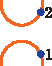
\includegraphics[scale=1]{CupCapDots.pdf}}}}}

\newcommand{\dbeta}{\mathord{\vcenter{\hbox{
\includegraphics[scale=1]{dbeta.pdf}}}}}
\newcommand{\dpsi}{\mathord{\vcenter{\hbox{
\includegraphics[scale=1]{dpsi.pdf}}}}}
\newcommand{\dblank}{\mathord{\vcenter{\hbox{
\includegraphics[scale=1]{dblank.pdf}}}}}





\newcommand{\SigmaDotDot}{\mathord{\vcenter{\hbox{
\includegraphics[scale=1]{SigmaDotDot.pdf}}}}}
\newcommand{\SigmaDotDotExchange}{\mathord{\vcenter{\hbox{
\includegraphics[scale=1]{SigmaDotDotExchange.pdf}}}}}
\newcommand{\TwoLine}{\mathord{\vcenter{\hbox{
\includegraphics[scale=1]{TwoLine.pdf}}}}}
\newcommand{\TwoLineDots}{\mathord{\vcenter{\hbox{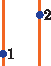
\includegraphics[scale=1]{TwoLineDots.pdf}}}}}


\newcommand{\RDotTwo}{\mathord{\vcenter{\hbox{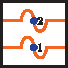
\includegraphics[scale=1]{RDotTwo.pdf}}}}}
\newcommand{\RDotTwoa}{\mathord{\vcenter{\hbox{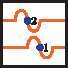
\includegraphics[scale=1]{RDotTwoa.pdf}}}}}
\newcommand{\RDotTwob}{\mathord{\vcenter{\hbox{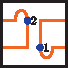
\includegraphics[scale=1]{RDotTwob.pdf}}}}}
\newcommand{\RDotTwoc}{\mathord{\vcenter{\hbox{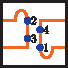
\includegraphics[scale=1]{RDotTwoc.pdf}}}}}

\newcommand{\FubeXXX}{\mathord{\vcenter{\hbox{
\includegraphics[scale=1]{EmptyTube.pdf}}}}}
\newcommand{\FubeXss}{\mathord{\vcenter{\hbox{
\includegraphics[scale=1]{OneLine.pdf}}}}}
\newcommand{\FubeXsds}{\mathord{\vcenter{\hbox{
\includegraphics[scale=1]{OneLineDot.pdf}}}}}



\newcommand{\AnnulusCut}{\mathord{\vcenter{\hbox{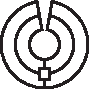
\includegraphics[scale=1]{AnnulusCut.pdf}}}}}
\newcommand{\AnnulusFlat}{\mathord{\vcenter{\hbox{
\includegraphics[scale=1]{AnnulusFlat.pdf}}}}}
\newcommand{\Disc}{\mathord{\vcenter{\hbox{
\includegraphics[scale=1]{Disc.pdf}}}}}
\newcommand{\RotatedTube}{\mathord{\vcenter{\hbox{
\includegraphics[scale=1]{RotatedTube.pdf}}}}}
\newcommand{\AnnulusGeneric}{\mathord{\vcenter{\hbox{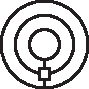
\includegraphics[scale=1]{AnnulusGeneric.pdf}}}}}



\newcommand{\FubeXXXA}{\mathord{\vcenter{\hbox{
\includegraphics[scale=1]{EmptyTubeA.pdf}}}}}
\newcommand{\FubeXssA}{\mathord{\vcenter{\hbox{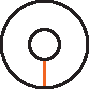
\includegraphics[scale=1]{OneLineA.pdf}}}}}
\newcommand{\FubeXsdsA}{\mathord{\vcenter{\hbox{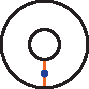
\includegraphics[scale=1]{OneLineDotA.pdf}}}}}

\newcommand{\FubesddXsA}{\mathord{\vcenter{\hbox{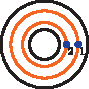
\includegraphics[scale=1]{FubesddXsA.pdf}}}}}

\newcommand{\RDotTwobA}{\mathord{\vcenter{\hbox{
\includegraphics[scale=1]{RDotTwobA.pdf}}}}}\newcommand{\RDotTwocA}{\mathord{\vcenter{\hbox{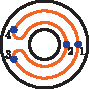
\includegraphics[scale=1]{RDotTwocA.pdf}}}}}


 
\newcommand{\Fubex}[2]{{\mathord{\ooalign{ \vphantom{$\Big|^2$}\cr\hidewidth\ensuremath{\scriptstyle{#2}}\hidewidth\cr$\vcenter{\hbox{$#1$}}$\cr
  \hidewidth\raise0ex\hbox{$\scale{1.2}{\VerticalSpace}$}\cr
  }}}}	




\newcommand{\TubeBC}{\mathord{\vcenter{\hbox{
\includegraphics[scale=1]{TubeBC.pdf}}}}}

\newcommand{\TubeBCx}[1]{{\mathord{\ooalign{ \vphantom{$\Big|^2$}\cr\hidewidth\ensuremath{\scriptstyle{#1}}\hidewidth\cr$\vcenter{\hbox{$\scale{1}{\TubeBC}$}}$\cr
  \hidewidth\raise0ex\hbox{$\scale{.25}{\VerticalSpace}$}\cr
  }}}}	

\newcommand{\AnnulusBare}{\mathord{\vcenter{\hbox{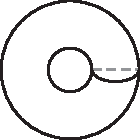
\includegraphics[scale=.6]{AnnulusBare.pdf}}}}}
\newcommand{\AnnularTube}{\mathord{\vcenter{\hbox{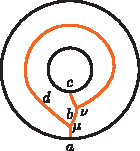
\includegraphics[scale=1]{AnnularTube.pdf}}}}}
\newcommand{\AnnularTubeNoIndex}{\mathord{\vcenter{\hbox{
\includegraphics[scale=1]{AnnularTubeNoIndex.pdf}}}}}
\newcommand{\AnnulusTubeTube}{\mathord{\vcenter{\hbox{
\includegraphics[scale=1]{AnnulusTubeTube.pdf}}}}}

\newcommand{\SAnnulusNoLabel}{\mathord{\vcenter{\hbox{
\includegraphics[scale=1]{SAnnulusNoLabel.pdf}}}}}
\newcommand{\TAnnulusNoLabel}{\mathord{\vcenter{\hbox{
\includegraphics[scale=1]{TAnnulusNoLabel.pdf}}}}}


\newcommand{\EdgeTensor}{\mathord{\vcenter{\hbox{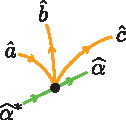
\includegraphics[scale=1]{EdgeTensor.pdf}}}}}

\newcommand{\OneHandleTheta}{\mathord{\vcenter{\hbox{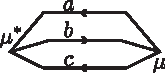
\includegraphics[scale=.7]{OneHandleTheta.pdf}}}}}
\newcommand{\OneHandlemud}{\mathord{\vcenter{\hbox{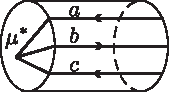
\includegraphics[scale=.7]{OneHandlemud.pdf}}}}}
\newcommand{\OneHandlemu}{\mathord{\vcenter{\hbox{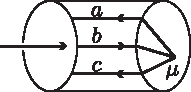
\includegraphics[scale=.7]{OneHandlemu.pdf}}}}}
\newcommand{\OneHandlea}{\mathord{\vcenter{\hbox{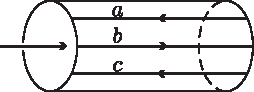
\includegraphics[scale=.7]{OneHandlea.pdf}}}}}

\newcommand{\Tetrahedron}{\mathord{\vcenter{\hbox{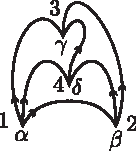
\includegraphics[scale=1]{Tetrahedron.pdf}}}}}
\newcommand{\PitchforkIdempotent}{\mathord{\vcenter{\hbox{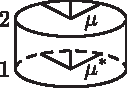
\includegraphics[scale=0.7]{PitchforkIdempotent.pdf}}}}}

\newcommand{\Pitchforkabc}{\mathord{\vcenter{\hbox{\includegraphics[scale=1]{Pitchforkabc.pdf}}}}}
\newcommand{\Pitchforkabcrot}{\mathord{\vcenter{\hbox{\includegraphics[scale=1]{Pitchforkabcrot.pdf}}}}}






\newcommand{\AnnulsLabel}[5]{\mathord{ 
\mkern2mu\overset{#3}{{\Annulusxprime{#1}{#2}}}\mkern2mu\raisebox{0ex}{$\scriptstyle{#4}$} }}

\newcommand*{\Annulus}[2]{{ #1 }
\kern-3.5em\raisebox{1ex}{ $\scriptstyle{#2}$} \kern2.6em} %Could change 0 to 1.2 to raise the B.

\newcommand*{\AnnulusP}[3]{{{\Annulus{#1}{#2}} }
\kern-.5em\raisebox{3.5ex}{ $\scriptstyle{#3}$} \kern.3em} %Could change 0 to 1.2 to raise the B.

\newcommand*{\AnnulusPx}[4]{\AnnulusP{#1}{#2}{#3}
\kern-3.6em\raisebox{-4.5ex}{ $\scriptstyle{#4}$} \kern2.6em} %Could change 0 to 1.2 to raise the B.

\newcommand*{\AnularTubex}[6]{\AnnulusPx{#1}{#2}{#3}{#4}
\kern-4em\raisebox{-4.5ex}{ $\overset{#6}{\underset{#5}{\vphantom{\Big|^2}}}$} \kern3em} %Could change 0 to 1.2 to raise the B.

\newcommand*{\TorusTubex}[6]{\AnnulusPx{#1}{#2}{#3}{#4}
\kern-4em\raisebox{-4.5ex}{ $\overset{#6}{\underset{#5}{\vphantom{\Big|^2}}}$} \kern3em} %Could change 0 to 1.2 to raise the B.

%\newcommand*{\AnnularTubex}[5]{\AnnulusPx{#1}{#2}{}{\; \; \;#3}
%\kern-3.9em\raisebox{-4.5ex}{ $\overset{#5}{\underset{#4}{\vphantom{\Big|^2}}}$} \kern2.7em} %Could change 0 to 1.2 to raise the B.



\newcommand{\SAnnulusx}[3]{\mathrel{\ooalign{$\SAnnulusNoLabel$\cr
  \hidewidth\raise5ex\hbox{$\scriptstyle{#3}\mkern1mu$}\cr
  \hidewidth\raise.8ex\hbox{$\scriptstyle{#2}\mkern63mu$}\cr
    \hidewidth\raise-3.8ex\hbox{$\scriptstyle{#1}\mkern39mu$}\cr
  }}}
  
  \newcommand{\TAnnulusx}[3]{\mathrel{\ooalign{$\TAnnulusNoLabel$\cr
  \hidewidth\raise5ex\hbox{$\scriptstyle{#3}\mkern1mu$}\cr
  \hidewidth\raise.8ex\hbox{$\scriptstyle{#2}\mkern63mu$}\cr
    \hidewidth\raise-4.9ex\hbox{$\scriptstyle{#1}\mkern51mu$}\cr
  }}}

\newcommand{\AnnularTubex}[6]{\mathrel{\ooalign{$#1$\cr
  \hidewidth\raise5ex\hbox{$\scriptstyle{#6}\mkern1mu$}\cr
  \hidewidth\raise.8ex\hbox{$\scriptstyle{#5}\mkern63mu$}\cr
  \hidewidth\raise-.9ex\hbox{$\scriptstyle{#3}\mkern68mu$}\cr
    \hidewidth\raise-4.5ex\hbox{$\scriptstyle{#4} \mkern50mu$}\cr
  \hidewidth\raise-7ex\hbox{$\scriptstyle{#2}\mkern68mu$}\cr
  }}}
  
%\newcommand{\AnnularTubexp}[9]{\mathrel{\ooalign{$#1$\cr
  %\hidewidth\raise5ex\hbox{$\scriptstyle{#9}\mkern1mu$}\cr
 %\hidewidth\raise.8ex\hbox{$\scriptstyle{#8}\mkern63mu$}\cr
 % \hidewidth\raise-3.4ex\hbox{$\scriptstyle{#7}\mkern68mu$}\cr
  %  \hidewidth\raise-5.1ex\hbox{$\scriptstyle{#6}\mkern80mu$}\cr
%  \hidewidth\raise-2.2ex\hbox{$\scriptstyle{#5}\mkern90mu$}\cr
 % \hidewidth\raise-.9ex\hbox{$\scriptstyle{#4}\mkern68mu$}\cr
%    \hidewidth\raise-4.5ex\hbox{$\scriptstyle{#3} \mkern50mu$}\cr
 % \hidewidth\raise-7ex\hbox{$\scriptstyle{#2}\mkern68mu$}\cr
 % }}}



\newcommand{\AnnularTubexp}[9]{\mathrel{\ooalign{$#1$\cr
  \hidewidth\raise5ex\hbox{$\scriptstyle{#9}\mkern1mu$}\cr
 \hidewidth\raise.8ex\hbox{$\scriptstyle{#8}\mkern63mu$}\cr
  \hidewidth\raise-3.7ex\hbox{$\scriptstyle{#7}\mkern50mu$}\cr
    \hidewidth\raise-5.1ex\hbox{$\scriptstyle{#6}\mkern57mu$}\cr
  \hidewidth\raise-2.2ex\hbox{$\scriptstyle{#5}\mkern90mu$}\cr
  \hidewidth\raise-.9ex\hbox{$\scriptstyle{#4}\mkern68mu$}\cr
    \hidewidth\raise-3.8ex\hbox{$\scriptstyle{#3} \mkern69mu$}\cr
  \hidewidth\raise-7ex\hbox{$\scriptstyle{#2}\mkern68mu$}\cr
  }}}


\newcommand{\SmallTorus}[3]{\mathrel{\ooalign{$#1$\cr
  \hidewidth\raise0ex\hbox{$\scriptstyle{#2}\mkern36mu$}\cr
    \hidewidth\raise-1.5ex\hbox{$\scriptstyle{#3}\mkern10mu$}\cr
  }}}
  
  
  \newcommand{\AnnulusTubeTubex}[6]{\mathrel{\ooalign{$#1$\cr
%  \hidewidth\raise5ex\hbox{$\scriptstyle{#7}\mkern1mu$}\cr
  \hidewidth\raise.8ex\hbox{$\scriptstyle{#6}\mkern65mu$}\cr
  \hidewidth\raise-.5ex\hbox{$\scriptstyle{#3}\mkern68mu$}\cr
    \hidewidth\raise-4.9ex\hbox{$\scriptstyle{#4} \mkern50mu$}\cr
     \hidewidth\raise-2.7ex\hbox{$\scriptstyle{#5} \mkern54mu$}\cr
  \hidewidth\raise-7.3ex\hbox{$\scriptstyle{#2}\mkern68mu$}\cr
  }}}
  

  \newcommand{\Cellup}{\mathord{\vcenter{\hbox{\includegraphics[scale=1]{Cellup.pdf}}}}}
    \newcommand{\Celldown}{\mathord{\vcenter{\hbox{\includegraphics[scale=1]{Celldown.pdf}}}}}
        \newcommand{\Cellmid}{\mathord{\vcenter{\hbox{\includegraphics[scale=1]{Cellmid.pdf}}}}}
        \newcommand{\TwoCell}{\mathord{\vcenter{\hbox{\includegraphics[scale=1]{TwoCell.pdf}}}}}
                \newcommand{\Onecell}{\mathord{\vcenter{\hbox{\includegraphics[scale=1]{Onecell.pdf}}}}}      
        
        

 


\newcommand{\TorusLocalRelationc}{\mathord{\vcenter{\hbox{\includegraphics[scale=1]{TorusLocalRelationc.pdf}}}}}
\newcommand{\TorusLocalRelationb}{\mathord{\vcenter{\hbox{\includegraphics[scale=1]{TorusLocalRelationb.pdf}}}}}
\newcommand{\TorusLocalRelationa}{\mathord{\vcenter{\hbox{\includegraphics[scale=1]{TorusLocalRelationa.pdf}}}}}


\newcommand{\Dv}{\mathord{\vcenter{\hbox{\includegraphics[scale=1]{Dv.pdf}}}}}
\newcommand{\Dfv}{\mathord{\vcenter{\hbox{\includegraphics[scale=1]{Dfv.pdf}}}}}


\newcommand{\Horseshoe}{\mathord{\vcenter{\hbox{\includegraphics[scale=1]{Horseshoe.pdf}}}}}
\newcommand{\HorseshoeTwist}{\mathord{\vcenter{\hbox{\includegraphics[scale=1]{HorseshoeTwist.pdf}}}}}
\newcommand{\euv}{\mathord{\vcenter{\hbox{\includegraphics[scale=1]{euv.pdf}}}}}
\newcommand{\chieuv}{\mathord{\vcenter{\hbox{\includegraphics[scale=1]{chieuv.pdf}}}}}


\newcommand{\TubeElement}{\mathord{\vcenter{\hbox{\includegraphics[scale=1]{TubeElement.pdf}}}}}


\newcommand{\LoopOverId}{\mathord{\vcenter{\hbox{\includegraphics[scale=1]{LoopOverId.pdf}}}}}
\newcommand{\Ida}{\mathord{\vcenter{\hbox{\includegraphics[scale=1]{Ida.pdf}}}}}
\newcommand{\OmegaSLoop}{\mathord{\vcenter{\hbox{\includegraphics[scale=1]{OmegaSLoop.pdf}}}}}

\newcommand{\IdxOmegaLoopa}{\mathord{\vcenter{\hbox{\includegraphics[scale=1]{IdxOmegaLoopa.pdf}}}}}
\newcommand{\IdxOmegaLoopb}{\mathord{\vcenter{\hbox{\includegraphics[scale=1]{IdxOmegaLoopb.pdf}}}}}


\newcommand{\HandleSlidea}{\mathord{\vcenter{\hbox{\includegraphics[scale=1]{HandleSlidea.pdf}}}}}
\newcommand{\HandleSlideb}{\mathord{\vcenter{\hbox{\includegraphics[scale=1]{HandleSlideb.pdf}}}}}


\newcommand{\TubeBasisa}{\mathord{\vcenter{\hbox{\includegraphics[scale=1]{TubeBasisa.pdf}}}}}
\newcommand{\TubeBasisb}{\mathord{\vcenter{\hbox{\includegraphics[scale=1]{TubeBasisb.pdf}}}}}
\newcommand{\TubeBasisc}{\mathord{\vcenter{\hbox{\includegraphics[scale=1]{TubeBasisc.pdf}}}}}
\newcommand{\TubeBasisd}{\mathord{\vcenter{\hbox{\includegraphics[scale=1]{TubeBasisd.pdf}}}}}
\newcommand{\TubeBasisdprime}{\mathord{\vcenter{\hbox{\includegraphics[scale=1]{TubeBasisdprime.pdf}}}}}


\newcommand{\gxyaj}{\mathord{\vcenter{\hbox{\includegraphics[scale=1]{gxyaj.pdf}}}}}
\newcommand{\hxyai}{\mathord{\vcenter{\hbox{\includegraphics[scale=1]{hxyai.pdf}}}}}

\newcommand{\VxyaoVxya}{\mathord{\vcenter{\hbox{\includegraphics[scale=1]{VxyaoVxya.pdf}}}}}
\newcommand{\idaprime}{\mathord{\vcenter{\hbox{\includegraphics[scale=1]{idaprime.pdf}}}}}

\newcommand{\Vxyxy}{\mathord{\vcenter{\hbox{\includegraphics[scale=1]{Vxyxy.pdf}}}}}
\newcommand{\idxy}{\mathord{\vcenter{\hbox{\includegraphics[scale=1]{idxy.pdf}}}}}
\newcommand{\Vxyxyomega}{\mathord{\vcenter{\hbox{\includegraphics[scale=1]{Vxyxyomega.pdf}}}}}



\newcommand{\SpinStructureProjector}{\mathord{\vcenter{\hbox{\includegraphics[scale=1]{SpinStructureProjector.pdf}}}}}


\newcommand{\EmptyTubeW}{\mathord{\vcenter{\hbox{\includegraphics[scale=1]{EmptyTubeW.pdf}}}}}

\newcommand{\TubeProject}{\mathord{\vcenter{\hbox{\includegraphics[scale=1]{TubeProject.pdf}}}}}


\newcommand{\TuberraJ}{\mathord{\vcenter{\hbox{\includegraphics[scale=1]{TuberraJ.pdf}}}}}
\newcommand{\Tubeidr}{\mathord{\vcenter{\hbox{\includegraphics[scale=1]{Tubeidr.pdf}}}}}
\newcommand{\Tuberr}{\mathord{\vcenter{\hbox{\includegraphics[scale=1]{Tuberr.pdf}}}}}


\newcommand{\TuberrTraceCe}{\mathord{\vcenter{\hbox{\includegraphics[scale=1]{TuberrTraceCe.pdf}}}}}
\newcommand{\TuberrTraceCo}{\mathord{\vcenter{\hbox{\includegraphics[scale=1]{TuberrTraceCo.pdf}}}}}



\newcommand{\exyomegaa}{\mathord{\vcenter{\hbox{\includegraphics[scale=1]{exyomegaa.pdf}}}}}
\newcommand{\exyomegab}{\mathord{\vcenter{\hbox{\includegraphics[scale=1]{exyomegab.pdf}}}}}
\newcommand{\exyomegac}{\mathord{\vcenter{\hbox{\includegraphics[scale=1]{exyomegac.pdf}}}}}

\newcommand{\EFunctora}{\mathord{\vcenter{\hbox{\includegraphics[scale=1]{EFunctora.pdf}}}}}
\newcommand{\EFunctorb}{\mathord{\vcenter{\hbox{\includegraphics[scale=1]{EFunctorb.pdf}}}}}
\newcommand{\EFunctorc}{\mathord{\vcenter{\hbox{\includegraphics[scale=1]{EFunctorc.pdf}}}}}



\newcommand{\TubeIdempotentTwoStrand}{\mathord{\vcenter{\hbox{\includegraphics[scale=1]{TubeIdempotentTwoStrand.pdf}}}}}
\newcommand{\fTubeCf}{\mathord{\vcenter{\hbox{\includegraphics[scale=1]{fTubeCf.pdf}}}}}
\newcommand{\fTubefOdd}{\mathord{\vcenter{\hbox{\includegraphics[scale=1]{fTubefOdd.pdf}}}}}
\newcommand{\minimalBosonic}{\mathord{\vcenter{\hbox{\includegraphics[scale=1]{minimalBosonic.pdf}}}}}



\newcommand{\FusionIsomorphism}{\mathord{\vcenter{\hbox{\includegraphics[scale=1]{FusionIsomorphism.pdf}}}}}


\newcommand{\TubeCompletea}{\mathord{\vcenter{\hbox{\includegraphics[scale=1]{TubeCompletea.pdf}}}}}
\newcommand{\TubeCompleteb}{\mathord{\vcenter{\hbox{\includegraphics[scale=1]{TubeCompleteb.pdf}}}}}
\newcommand{\TubeCompletec}{\mathord{\vcenter{\hbox{\includegraphics[scale=1]{TubeCompletec.pdf}}}}}
\newcommand{\TubeCompletecprime}{\mathord{\vcenter{\hbox{\includegraphics[scale=1]{TubeCompletecprime.pdf}}}}}



\newcommand{\Ufghk}{\mathord{\vcenter{\hbox{\includegraphics[scale=1]{Ufghk.pdf}}}}}


\newcommand{\fxyaJ}{\mathord{\vcenter{\hbox{\includegraphics[scale=1]{fxyaJ.pdf}}}}}


\newcommand{\TubeTwotoOneStrand}{\mathord{\vcenter{\hbox{\includegraphics[scale=1]{TubeTwotoOneStrand.pdf}}}}}
\newcommand{\TubeOnetoTwoStrand}{\mathord{\vcenter{\hbox{\includegraphics[scale=1]{TubeOnetoTwoStrand.pdf}}}}}
 

\newcommand{\SMatrix}[2]{\mathrel{\ooalign{$\OmegaSLoop$\cr
  \hidewidth\raise0ex\hbox{$\scriptstyle{#1}\mkern18mu$}\cr
    \hidewidth\raise0ex\hbox{$\scriptstyle{#2}\mkern-10mu$}\cr
  }}}
  
  
  \newcommand{\SMatrixx}[2]{\mathrel{\ooalign{$\OmegaSLoop$\cr
  \hidewidth\raise0ex\hbox{$\scriptstyle{#1}\mkern12mu$}\cr
    \hidewidth\raise0ex\hbox{$\scriptstyle{#2}\mkern-10mu$}\cr
  }}}
  
  \newcommand{\OmegaLoopDefectx}[2]{\mathrel{\ooalign{$\OmegaLoopDefect$\cr
  \hidewidth\raise0ex\hbox{$\scriptstyle{#1}\mkern8mu$}\cr
    \hidewidth\raise0ex\hbox{$\scriptstyle{#2}\mkern-22mu$}\cr
  }}}
  
  \newcommand{\OmegaLoopDefect}{\mathord{\vcenter{\hbox{\includegraphics[scale=1]{OmegaLoopDefect.pdf}}}}}
    \newcommand{\DiscGray}{\mathord{\vcenter{\hbox{\includegraphics[scale=1]{DiscGray.pdf}}}}}
    
    
    
\newcommand{\DCSmatrixf}{\mathord{\vcenter{\hbox{\includegraphics[scale=1]{DCSmatrixf.pdf}}}}}
\newcommand{\DCSmatrixa}{\mathord{\vcenter{\hbox{\includegraphics[scale=1]{DCSmatrixa.pdf}}}}}
\newcommand{\DCSmatrixb}{\mathord{\vcenter{\hbox{\includegraphics[scale=1]{DCSmatrixb.pdf}}}}}\newcommand{\DCSmatrixc}{\mathord{\vcenter{\hbox{\includegraphics[scale=1]{DCSmatrixc.pdf}}}}}
\newcommand{\DCSmatrixd}{\mathord{\vcenter{\hbox{\includegraphics[scale=1]{DCSmatrixd.pdf}}}}}
\newcommand{\DCSmatrixe}{\mathord{\vcenter{\hbox{\includegraphics[scale=1]{DCSmatrixe.pdf}}}}}

\newcommand{\DCSmatrixg}{\mathord{\vcenter{\hbox{\includegraphics[scale=1]{DCSmatrixg.pdf}}}}}
\newcommand{\DCSmatrixh}{\mathord{\vcenter{\hbox{\includegraphics[scale=1]{DCSmatrixh.pdf}}}}}


\newcommand{\STorusBasisa}{\mathord{\vcenter{\hbox{\includegraphics[scale=1]{STorusBasisa.pdf}}}}}


\newcommand{\Scalcae}{\mathord{\vcenter{\hbox{\includegraphics[scale=1]{Scalcae.pdf}}}}}  
\newcommand{\Scalcad}{\mathord{\vcenter{\hbox{\includegraphics[scale=1]{Scalcad.pdf}}}}}  
\newcommand{\Scalcac}{\mathord{\vcenter{\hbox{\includegraphics[scale=1]{Scalcac.pdf}}}}}  
\newcommand{\Scalcab}{\mathord{\vcenter{\hbox{\includegraphics[scale=1]{Scalcab.pdf}}}}}
\newcommand{\Scalcaa}{\mathord{\vcenter{\hbox{\includegraphics[scale=1]{Scalcaa.pdf}}}}}  


\newcommand{\Scalcbe}{\mathord{\vcenter{\hbox{\includegraphics[scale=1]{Scalcbe.pdf}}}}}  
\newcommand{\Scalcbd}{\mathord{\vcenter{\hbox{\includegraphics[scale=1]{Scalcbd.pdf}}}}}  
\newcommand{\Scalcbc}{\mathord{\vcenter{\hbox{\includegraphics[scale=1]{Scalcbc.pdf}}}}}  
\newcommand{\Scalcbb}{\mathord{\vcenter{\hbox{\includegraphics[scale=1]{Scalcbb.pdf}}}}}
\newcommand{\Scalcba}{\mathord{\vcenter{\hbox{\includegraphics[scale=1]{Scalcba.pdf}}}}}  


\newcommand{\Scalcbedot}{\mathord{\vcenter{\hbox{\includegraphics[scale=1]{Scalcbedot.pdf}}}}}  
\newcommand{\Scalcbddot}{\mathord{\vcenter{\hbox{\includegraphics[scale=1]{Scalcbddot.pdf}}}}}  
\newcommand{\Scalcbadot}{\mathord{\vcenter{\hbox{\includegraphics[scale=1]{Scalcbadot.pdf}}}}}    
  

  
%\newcommand{\SMatrix}[2]{\mathrel{\ooalign{$\OmegaSLoop$
%\mathrel{\raisebox{#1}{$\oldsqsubset$}}
  %\hidewidth\raise0ex\hbox{$\scriptstyle{a}\mkern0mu$}\cr
    %\hidewidth\raise0ex\hbox{$\scriptstyle{b}\mkern0mu$}\cr
%    \hidewidth\raise-4.3ex\hbox{$\scriptstyle{#2}\mkern43mu$}\cr
%        \hidewidth\raise-6.3ex\hbox{$\scriptstyle{#2}\mkern61mu$}\cr
%        \hidewidth\raise4.1ex\hbox{$\scriptstyle{#4}\mkern25mu$}\cr
  %              \hidewidth\raise-0.3ex\hbox{$\scriptstyle{#3}\mkern60mu$}\cr
%          \hidewidth\raise0ex\hbox{$\scale{1.5}{\VerticalSpace}$}\cr
 %}}}
 
 
\newcommand{\LoopArrow}{\mathord{\vcenter{\hbox{\includegraphics[scale=1]{LoopArrow.pdf}}}}}  
\newcommand{\LoopArrowx}[1]{\mathrel{\ooalign{$\LoopArrow_{\mathrel{\raisebox{4pt}{$\scriptstyle{#1}$}}}$
  }}}
  
  
\newcommand{\OmegaLoop}{\mathord{\vcenter{\hbox{\includegraphics[scale=1]{OmegaLoop.pdf}}}}}  
\newcommand{\OmegaLoopx}[1]{\mathrel{\ooalign{$\OmegaLoop_{\mathrel{\raisebox{4pt}{$\scriptstyle{#1}$}}}$
  }}}



\newcommand{\TubeElementx}[3]{\mathrel{\ooalign{$\TubeElement$\cr
  \hidewidth\raise-3.55ex\hbox{$\scriptstyle{#1}\mkern62mu$}\cr
%    \hidewidth\raise-4.3ex\hbox{$\scriptstyle{#2}\mkern43mu$}\cr
        \hidewidth\raise-6.3ex\hbox{$\scriptstyle{#2}\mkern61mu$}\cr
%        \hidewidth\raise4.1ex\hbox{$\scriptstyle{#4}\mkern25mu$}\cr
                \hidewidth\raise-0.3ex\hbox{$\scriptstyle{#3}\mkern60mu$}\cr
          \hidewidth\raise0ex\hbox{$\scale{1.5}{\VerticalSpace}$}\cr
  }}}

\newcommand{\IdempotentMTCNoLabel}{\mathord{\vcenter{\hbox{\includegraphics[scale=1]{IdempotentMTC.pdf}}}}}
\newcommand{\IdempBraid}[5]{\mathrel{\ooalign{$\IdempotentMTCNoLabel$\cr
  \hidewidth\raise-4.3ex\hbox{$\scriptstyle{#1}\mkern78mu$}\cr
    \hidewidth\raise-4.3ex\hbox{$\scriptstyle{#2}\mkern43mu$}\cr
        \hidewidth\raise-6.3ex\hbox{$\scriptstyle{#3}\mkern61mu$}\cr
        \hidewidth\raise4.1ex\hbox{$\scriptstyle{#4}\mkern25mu$}\cr
                \hidewidth\raise0ex\hbox{$\scriptstyle{#5}\mkern60mu$}\cr
          \hidewidth\raise0ex\hbox{$\scale{1.5}{\VerticalSpace}$}\cr
  }}}
  
\newcommand{\TorusBasisMTCNoLabel}{\mathord{\vcenter{\hbox{\includegraphics[scale=1]{TorusBasisMTC.pdf}}}}}
\newcommand{\TorusBraidBasis}[6]{\mathrel{\ooalign{$\TorusBasisMTCNoLabel$\cr
  \hidewidth\raise-4.3ex\hbox{$\scriptstyle{#1}\mkern78mu$}\cr
    \hidewidth\raise-4.3ex\hbox{$\scriptstyle{#2}\mkern40mu$}\cr
        \hidewidth\raise-6.3ex\hbox{$\scriptstyle{#3}\mkern61mu$}\cr
        \hidewidth\raise4.1ex\hbox{$\scriptstyle{#4}\mkern25mu$}\cr
                \hidewidth\raise0ex\hbox{$\scriptstyle{#5}\mkern58mu$}\cr
                                \hidewidth\raise4.7ex\hbox{$\scriptstyle{#6}\mkern0mu$}\cr
          \hidewidth\raise0ex\hbox{$\scale{1.5}{\VerticalSpace}$}\cr
  }}}
  
  \newcommand{\tcca}{\mathord{\vcenter{\hbox{\includegraphics[scale=1]{tcca.pdf}}}}}
    \newcommand{\tccb}{\mathord{\vcenter{\hbox{\includegraphics[scale=1]{tccb.pdf}}}}}
     \newcommand{\tccc}{\mathord{\vcenter{\hbox{\includegraphics[scale=1]{tccc.pdf}}}}}
      \newcommand{\tccd}{\mathord{\vcenter{\hbox{\includegraphics[scale=1]{tccd.pdf}}}}}
   
  
 


\newcommand{\TorusBasisMTCdl}{\mathord{\vcenter{\hbox{\includegraphics[scale=1]{TorusBasisMTCdl.pdf}}}}}
\newcommand{\TorusBasisMTCdr}{\mathord{\vcenter{\hbox{\includegraphics[scale=1]{TorusBasisMTCdr.pdf}}}}}
\newcommand{\TorusBasisMTCdd}{\mathord{\vcenter{\hbox{\includegraphics[scale=1]{TorusBasisMTCdd.pdf}}}}}
 
 \newcommand{\TorusBraidBasisd}[7]{\mathrel{\ooalign{$#7$\cr
  \hidewidth\raise-4.3ex\hbox{$\scriptstyle{#1}\mkern78mu$}\cr
    \hidewidth\raise-4.3ex\hbox{$\scriptstyle{#2}\mkern40mu$}\cr
        \hidewidth\raise-6.3ex\hbox{$\scriptstyle{#3}\mkern61mu$}\cr
        \hidewidth\raise4.1ex\hbox{$\scriptstyle{#4}\mkern25mu$}\cr
                \hidewidth\raise0ex\hbox{$\scriptstyle{#5}\mkern58mu$}\cr
                                \hidewidth\raise4.7ex\hbox{$\scriptstyle{#6}\mkern0mu$}\cr
          \hidewidth\raise0ex\hbox{$\scale{1.5}{\VerticalSpace}$}\cr
  }}}



\newcommand{\TaddownTubeNoLabel}{\mathord{\vcenter{\hbox{\includegraphics[scale=1]{TaddownTube.pdf}}}}}
\newcommand{\TadupTubeNoLabel}{\mathord{\vcenter{\hbox{\includegraphics[scale=1]{TadupTube.pdf}}}}}
\newcommand{\hTube}{\mathord{\vcenter{\hbox{\includegraphics[scale=1]{hTube.pdf}}}}}
\newcommand{\tTube}{\mathord{\vcenter{\hbox{\includegraphics[scale=1]{tTube.pdf}}}}}
\newcommand{\eTube}{\mathord{\vcenter{\hbox{\includegraphics[scale=1]{eTube.pdf}}}}}
\newcommand{\vTube}{\mathord{\vcenter{\hbox{\includegraphics[scale=1]{vTube.pdf}}}}}


\newcommand{\dota}{\mathord{\vcenter{\hbox{\includegraphics[scale=1]{dota.pdf}}}}}
\newcommand{\dotb}{\mathord{\vcenter{\hbox{\includegraphics[scale=1]{dotb.pdf}}}}}
\newcommand{\dotc}{\mathord{\vcenter{\hbox{\includegraphics[scale=1]{dotc.pdf}}}}}

\newcommand{\XTubeNoLabel}{\mathord{\vcenter{\hbox{\includegraphics[scale=1]{XTube.pdf}}}}}
\newcommand{\XTube}[2]{\mathrel{\ooalign{$\XTubeNoLabel$\cr
  \hidewidth\raise-2.5ex\hbox{$\scriptstyle{#2}\mkern28mu$}\cr
    \hidewidth\raise-2.9ex\hbox{$\scriptstyle{#1}\mkern50mu$}\cr
  }}}


\newcommand{\TaddownTube}[1]{\mathrel{\ooalign{$\TaddownTubeNoLabel$\cr
    \hidewidth\raise-2.8ex\hbox{$\scriptstyle{#1}\mkern30mu$}\cr
  }}}
  \newcommand{\TadupTube}[1]{\mathrel{\ooalign{$\TadupTubeNoLabel$\cr
    \hidewidth\raise-2.6ex\hbox{$\scriptstyle{#1}\mkern30mu$}\cr
  }}}
  
  \newcommand{\TorusNoLabels}{\mathord{\vcenter{\hbox{\includegraphics[scale=1]{TorusNoLabels.pdf}}}}}
\newcommand{\TorusNoLabelsx}[1]{\mathrel{\ooalign{$\TorusNoLabels$\cr
    \hidewidth\raise-2.8ex\hbox{$\scriptstyle{#1}\mkern30mu$}\cr
  }}}

\newcommand{\VerticalSpace}{\mathord{\vcenter{\hbox{\includegraphics[scale=1]{VerticalSpace.pdf}}}}}

\newcommand{\AddDat}[3]{\mathrel{\ooalign{  $#1$\cr
  \hidewidth\raise0ex\hbox{$\scriptstyle{#2}\mkern38mu$}\cr
  \hidewidth\raise0ex\hbox{${#3}\mkern0mu$}\cr
  \hidewidth\raise0ex\hbox{$\VerticalSpace$}\cr
  }}}
  
  \newcommand{\AddDatTorus}[3]{\mathrel{\ooalign{  $#1$\cr
  \hidewidth\raise0ex\hbox{$\scriptstyle{#2}\mkern38mu$}\cr
  \hidewidth\raise3.8ex\hbox{$\scriptstyle{#3}\mkern0mu$}\cr
  \hidewidth\raise0ex\hbox{$\VerticalSpace$}\cr
  }}}
  
    \newcommand{\AddDatTorusDot}[4]{\mathrel{\ooalign{  $#1$\cr
  \hidewidth\raise0ex\hbox{$\scriptstyle{#2}\mkern38mu$}\cr
  \hidewidth\raise3.8ex\hbox{$\scriptstyle{#3}\mkern0mu$}\cr
  \hidewidth\raise0ex\hbox{${#4}\mkern0mu$}\cr
  \hidewidth\raise0ex\hbox{$\VerticalSpace$}\cr
  }}}
  
  
  
 
  
   
  \newcommand{\TubeProductCoefficienta}{\mathord{\vcenter{\hbox{\includegraphics[scale=1]{TubeProductCoefficienta.pdf}}}}}
  \newcommand{\TubeProductCoefficientb}{\mathord{\vcenter{\hbox{\includegraphics[scale=1]{TubeProductCoefficientb.pdf}}}}}
  
    \newcommand{\ThetaSymbol}{\mathord{\vcenter{\hbox{\includegraphics[scale=1]{Theta.pdf}}}}}
 
   \newcommand{\ThetaSymbolx}[1]{\mathrel{\ooalign{$\ThetaSymbol$\cr
      \hidewidth\raise-1.3ex\hbox{$\scriptstyle{#1} \mkern0mu$}\cr
  }}}
  
  
    
  \newcommand{\TubeProductCoefficientbx}[2]{\mathrel{\ooalign{$\TubeProductCoefficientb \;\;\; $\cr
      \hidewidth\raise-.8ex\hbox{$\scriptstyle{#1} \mkern54mu$}\cr
      \hidewidth\raise-.8ex\hbox{$\scriptstyle{#2} \mkern6mu$}\cr
  }}}
  
  \newcommand{\TubeProductCoefficientax}[5]{\mathrel{\ooalign{$\TubeProductCoefficienta$\cr
      \hidewidth\raise-4.2ex\hbox{$\scriptstyle{#1} \mkern30mu$}\cr
      \hidewidth\raise-1.8ex\hbox{$\scriptstyle{#2} \mkern30mu$}\cr
  \hidewidth\raise6.1ex\hbox{$\scriptstyle{#3}\mkern44mu$}\cr
  \hidewidth\raise2.05ex\hbox{$\scriptstyle{#4}\mkern82mu$}\cr
    \hidewidth\raise3.2ex\hbox{$\scriptstyle{#5}\mkern3mu$}\cr
  }}}

  

  
    
\newcommand{\tubex}[8]{#1 \left(\substack{#8\\ \\ #5\\ } \; \substack{#4\\ #3\\ #2\\ }\; \substack{ #7 \\ #6} \right)}
%\newcommand*{\SmallTorus}[3]{\kern 2.05 em\raisebox{0ex}{ $\scriptstyle{#2}$} \kern-2.05em{ #1 } 
%\kern-1.1em\raisebox{-1.5ex}{$\scriptstyle{#3}$} \kern1.1em} %Could change 0 to 1.2 to raise the B.


%\newcommand*{\Tubex}[2]{{ \AnnularTube }
%\kern-3.5em\raisebox{1ex}{ $\scriptstyle{#2}$} \kern3.5em} %Could change 0 to 1.2 to raise the B.


%\newcommand{\BWfour}[5]{\mathord{ \raisebox{0.2ex}{$\scriptstyle{#2}$}\mkern2mu\overset{#3}{\underset{#4}{#1}}\mkern2mu\raisebox{0.2ex}{$\scriptstyle{#5}$} }}




\newcommand{\FubesXs}{\mathord{\vcenter{\hbox{\includegraphics[scale=1,angle=90,origin=c]{OneLine.pdf}}}}}
\newcommand{\FubesdXs}{\mathord{\vcenter{\hbox{\includegraphics[scale=1]{FubesdXs.pdf}}}}}

\newcommand{\FubessX}{\mathord{\vcenter{\hbox{\includegraphics[scale=1]{FubessX.pdf}}}}}
\newcommand{\FubessdX}{\mathord{\vcenter{\hbox{\includegraphics[scale=1]{FubessdX.pdf}}}}}

\newcommand{\FubesdXsA}{\mathord{\vcenter{\hbox{\includegraphics[scale=1]{FubesdXsA.pdf}}}}}
\newcommand{\FubessXA}{\mathord{\vcenter{\hbox{\includegraphics[scale=1]{FubessXA.pdf}}}}}
\newcommand{\FubessdXA}{\mathord{\vcenter{\hbox{\includegraphics[scale=1]{FubessdXA.pdf}}}}}


\newcommand{\FubesXsA}{\mathord{\vcenter{\hbox{\includegraphics[scale=1]{FubesXshA.pdf}}}}}
\newcommand{\FubesXsa}{\mathord{\vcenter{\hbox{\includegraphics[scale=1]{FubesXsa.pdf}}}}}
\newcommand{\FubesXsb}{\mathord{\vcenter{\hbox{\includegraphics[scale=1]{FubesXsb.pdf}}}}}
\newcommand{\FubesXsc}{\mathord{\vcenter{\hbox{\includegraphics[scale=1]{FubesXsc.pdf}}}}}


\newcommand{\FubesXscA}{\mathord{\vcenter{\hbox{\includegraphics[scale=1]{FubeXscA.pdf}}}}}
\newcommand{\FubesXsbA}{\mathord{\vcenter{\hbox{\includegraphics[scale=1]{FubeXsbA.pdf}}}}}
\newcommand{\FubesXsaA}{\mathord{\vcenter{\hbox{\includegraphics[scale=1]{FubeXsaA.pdf}}}}}






\newcommand{\qqo}{\mathord{\vcenter{\hbox{\includegraphics[scale=.4]{qq1.pdf}}}}}
\newcommand{\qtqo}{\mathord{\vcenter{\hbox{\includegraphics[scale=.4]{qtq1.pdf}}}}}
\newcommand{\qqto}{\mathord{\vcenter{\hbox{\includegraphics[scale=.4]{qqt1.pdf}}}}}
\newcommand{\qtqto}{\mathord{\vcenter{\hbox{\includegraphics[scale=.4]{qtqt1.pdf}}}}}
\newcommand{\qqm}{\mathord{\vcenter{\hbox{\includegraphics[scale=.4]{qqm.pdf}}}}}
\newcommand{\qtqm}{\mathord{\vcenter{\hbox{\includegraphics[scale=.4]{qtqm.pdf}}}}}
\newcommand{\qqtm}{\mathord{\vcenter{\hbox{\includegraphics[scale=.4]{qqtm.pdf}}}}}
\newcommand{\qtqtm}{\mathord{\vcenter{\hbox{\includegraphics[scale=.4]{qtqtm.pdf}}}}}

\newcommand{\PantsPAP}{\mathord{\vcenter{\hbox{\includegraphics[scale=0.7]{PantsPAP.pdf}}}}}
\newcommand{\PantsPAsP}{\mathord{\vcenter{\hbox{\includegraphics[scale=0.7]{PantsPAsP.pdf}}}}}

\newcommand{\PantsPsdAP}{\mathord{\vcenter{\hbox{\includegraphics[scale=0.7]{PantsPsdAP.pdf}}}}}
\newcommand{\PantsPsdAsP}{\mathord{\vcenter{\hbox{\includegraphics[scale=0.7]{PantsPsdAsP.pdf}}}}}



\newcommand{\PantsPPA}{\mathord{\vcenter{\hbox{\includegraphics[scale=0.7]{PantsPPA.pdf}}}}}
\newcommand{\PantsPPAs}{\mathord{\vcenter{\hbox{\includegraphics[scale=0.7]{PantsPPAs.pdf}}}}}

\newcommand{\PantsAsAshAsvt}{\mathord{\vcenter{\hbox{\includegraphics[scale=0.7]{PantsAsAshAsvt.pdf}}}}}
\newcommand{\PantsAstAAs}{\mathord{\vcenter{\hbox{\includegraphics[scale=0.7]{PantsAstAAs.pdf}}}}}

\newcommand{\PantsAstAshAs}{\mathord{\vcenter{\hbox{\includegraphics[scale=0.7]{PantsAstAshAs.pdf}}}}}
\newcommand{\PantsAsAshAs}{\mathord{\vcenter{\hbox{\includegraphics[scale=0.7]{PantsAsAshAs.pdf}}}}}
\newcommand{\PantsAsAAs}{\mathord{\vcenter{\hbox{\includegraphics[scale=0.7]{PantsAsAAs.pdf}}}}}

\newcommand{\Pantssvtsvtsh}{\mathord{\vcenter{\hbox{\includegraphics[scale=.7,origin=c]{Pantssvtsvtsh.pdf}}}}}
\newcommand{\Pantssvtsvsh}{\mathord{\vcenter{\hbox{\includegraphics[scale=.7,angle=0,origin=c]{Pantssvtsvsh.pdf}}}}}
\newcommand{\Pantssvsvtsh}{\mathord{\vcenter{\hbox{\includegraphics[scale=.7,angle=0,origin=c]{Pantssvsvtsh.pdf}}}}}
\newcommand{\Pantssvsvsh}{\mathord{\vcenter{\hbox{\includegraphics[scale=.7,angle=0,origin=c]{Pantssvsvsh.pdf}}}}}
\newcommand{\PantssvtsvtX}{\mathord{\vcenter{\hbox{\includegraphics[scale=.7,angle=0,origin=c]{PantssvtsvtX.pdf}}}}}
\newcommand{\PantssvtsvX}{\mathord{\vcenter{\hbox{\includegraphics[scale=.7,angle=0,origin=c]{PantssvtsvX.pdf}}}}}
%\newcommand{\PantssvtsvX}{\mathord{\vcenter{\hbox{\includegraphics[scale=.7,angle=0,origin=c]{PantssvtsvX.pdf}}}}}
\newcommand{\PantssvsvtX}{\mathord{\vcenter{\hbox{\includegraphics[scale=.7,angle=0,origin=c]{PantssvsvtX.pdf}}}}}
\newcommand{\PantssvsvX}{\mathord{\vcenter{\hbox{\includegraphics[scale=.7,angle=0,origin=c]{PantssvsvX.pdf}}}}}

\newcommand{\PantssvtXsvd}{\mathord{\vcenter{\hbox{\includegraphics[scale=.7,angle=0,origin=c]{PantssvtXsvd.pdf}}}}}
\newcommand{\Pantssvtshsvd}{\mathord{\vcenter{\hbox{\includegraphics[scale=.7,angle=0,origin=c]{Pantssvtshsvd.pdf}}}}}
\newcommand{\Pantssvshsvd}{\mathord{\vcenter{\hbox{\includegraphics[scale=.7,angle=0,origin=c]{Pantssvshsvd.pdf}}}}}
\newcommand{\PantssvXsvd}{\mathord{\vcenter{\hbox{\includegraphics[scale=.7,angle=0,origin=c]{PantssvXsvd.pdf}}}}}

\newcommand{\PantssvtXsvt}{\mathord{\vcenter{\hbox{\includegraphics[scale=.7,angle=0,origin=c]{PantssvtXsvt.pdf}}}}}
\newcommand{\PantssvXsvt}{\mathord{\vcenter{\hbox{\includegraphics[scale=.7,angle=0,origin=c]{PantssvXsvt.pdf}}}}}

\newcommand{\PantssvtXsv}{\mathord{\vcenter{\hbox{\includegraphics[scale=.7,angle=0,origin=c]{PantssvtXsv.pdf}}}}}



%%%%%%%%%%%%%%%%%%%%%%%%%%%%%%%%%%%%%%%%%%%%%%%%
%%%%%%%%%%%%%%%%%%%%%%%%%%%%%%%%%%%%%%%%%%%%%%%%
\newcommand{\PantssvXsvdA}{\mathord{\vcenter{\hbox{\includegraphics[scale=.8,angle=0,origin=c]{PantssvXsvdA.pdf}}}}}
\newcommand{\PantssvtXsvdA}{\mathord{\vcenter{\hbox{\includegraphics[scale=.8,angle=0,origin=c]{PantssvtXsvdA.pdf}}}}}
\newcommand{\PantssvtshsvdA}{\mathord{\vcenter{\hbox{\includegraphics[scale=.8,angle=0,origin=c]{PantssvtshsvdA.pdf}}}}}
\newcommand{\PantssvshsvdA}{\mathord{\vcenter{\hbox{\includegraphics[scale=.8,angle=0,origin=c]{PantssvshsvdA.pdf}}}}}
\newcommand{\PantsPsdAsPA}{\mathord{\vcenter{\hbox{\includegraphics[scale=.8,angle=0,origin=c]{PantsPsdAsPA.pdf}}}}}
\newcommand{\PantsPsdAPA}{\mathord{\vcenter{\hbox{\includegraphics[scale=.8,angle=0,origin=c]{PantsPsdAPA.pdf}}}}}
\newcommand{\PantsPPAsA}{\mathord{\vcenter{\hbox{\includegraphics[scale=.8,angle=0,origin=c]{PantsPPAsA.pdf}}}}}
\newcommand{\PantsPPAA}{\mathord{\vcenter{\hbox{\includegraphics[scale=.8,angle=0,origin=c]{PantsPPAA.pdf}}}}}
\newcommand{\PantsPAsPA}{\mathord{\vcenter{\hbox{\includegraphics[scale=.8,angle=0,origin=c]{PantsPAsPA.pdf}}}}}
\newcommand{\PantsPAPA}{\mathord{\vcenter{\hbox{\includegraphics[scale=.8,angle=0,origin=c]{PantsPAPA.pdf}}}}}
\newcommand{\PantsAstAAsA}{\mathord{\vcenter{\hbox{\includegraphics[scale=.8,angle=0,origin=c]{PantsAstAAsA.pdf}}}}}
\newcommand{\PantsAsAshAsvtA}{\mathord{\vcenter{\hbox{\includegraphics[scale=.8,angle=0,origin=c]{PantsAsAshAsvtA.pdf}}}}}
\newcommand{\PantsNNda}{\mathord{\vcenter{\hbox{\includegraphics[scale=.8,angle=0,origin=c]{PantsNNda.pdf}}}}}
\newcommand{\PantsNNd}{\mathord{\vcenter{\hbox{\includegraphics[scale=.8,angle=0,origin=c]{PantsNNd.pdf}}}}}
%%%%%%%%%%%%%%%%%%%%%%%%%%%%%%%%%%%%%%%%%%%%%%%%
%%%%%%%%%%%%%%%%%%%%%%%%%%%%%%%%%%%%%%%%%%%%%%%%

\newcommand{\TwoLinedotdot}{\mathord{\vcenter{\hbox{\includegraphics[scale=1.5,angle=0,origin=c]{TwoLinedotdot.pdf}}}}}

\newcommand{\Id}{\mathord{\vcenter{\hbox{\includegraphics[scale=1.5,angle=0,origin=c]{Id.pdf}}}}}

\newcommand{\CupSigmadot}{\mathord{\vcenter{\hbox{\includegraphics[scale=1.5,angle=0,origin=c]{Cupdot.pdf}}}}}

\newcommand{\CupSigma}{\mathord{\vcenter{\hbox{\includegraphics[scale=1.5,angle=0,origin=c]{Cup.pdf}}}}}

\newcommand{\StaggaredGSOdd}{\mathord{\vcenter{\hbox{\includegraphics[scale=1.5,angle=0,origin=c]{StaggaredGSOdd.pdf}}}}}
\newcommand{\StaggaredGSEven}{\mathord{\vcenter{\hbox{\includegraphics[scale=1.5,angle=0,origin=c]{StaggeredGSEven.pdf}}}}}

\newcommand{\StaggaredGSEvenR}{\mathord{\vcenter{\hbox{\reflectbox{\includegraphics[scale=1.5,angle=0,origin=c]{StaggeredGSEven.pdf}}}}}}





\newcommand{\VxsdsY}{\mathord{\vcenter{\hbox{\includegraphics[scale=0.3,angle=0,origin=c]{Vxsds.pdf}}}}}
\newcommand{\VsdxsY}{\mathord{\vcenter{\hbox{\includegraphics[scale=0.3,angle=0,origin=c]{Vsdxs.pdf}}}}}
\newcommand{\VtssdxY}{\mathord{\vcenter{\hbox{\includegraphics[scale=0.3,angle=0,origin=c]{Vtssdx.pdf}}}}}

\newcommand{\Vssdx}{\mathord{\vcenter{\hbox{\includegraphics[scale=0.3,angle=0,origin=c]{Vssdx.pdf}}}}}
\newcommand{\Vxsds}{\mathord{\vcenter{\hbox{\reflectbox{\includegraphics[scale=0.3,angle=0,origin=c]{Vssdx.pdf}}}}}}

\newcommand{\Vssx}{\mathord{\vcenter{\hbox{\includegraphics[scale=0.3,angle=0,origin=c]{Vssx.pdf}}}}}
\newcommand{\Vxss}{\mathord{\vcenter{\hbox{\reflectbox{\includegraphics[scale=0.3,angle=0,origin=c]{Vssx.pdf}}}}}}

\newcommand{\Vsxs}{\mathord{\vcenter{\hbox{\includegraphics[scale=0.3,angle=0,origin=c]{Vsxs.pdf}}}}}
\newcommand{\Vsxsd}{\mathord{\vcenter{\hbox{\includegraphics[scale=0.3,angle=0,origin=c]{Vsxsd.pdf}}}}}

\newcommand{\VsxsY}{\mathord{\vcenter{\hbox{\includegraphics[scale=0.3,angle=180,origin=c]{Vsxs.pdf}}}}}
\newcommand{\VssxY}{\mathord{\vcenter{\hbox{\includegraphics[scale=0.3,angle=180,origin=c]{Vssx.pdf}}}}}
\newcommand{\VxssY}{\mathord{\vcenter{\hbox{\reflectbox{\includegraphics[scale=0.3,angle=180,origin=c]{Vssx.pdf}}}}}}

\newcommand{\PsiFermion}{\mathord{\vcenter{\hbox{\includegraphics[scale=1.5]{PsiFermion.pdf}}}}}
\newcommand{\PsiFermionTwist}{\mathord{\vcenter{\hbox{\includegraphics[scale=1.5]{PsiFermionTwist.pdf}}}}}

\newcommand{\TwoFermion}{\mathord{\vcenter{\hbox{\includegraphics[scale=1.5]{TwoFermion.pdf}}}}}
\newcommand{\TwoFermionExchange}{\mathord{\vcenter{\hbox{\includegraphics[scale=1.5]{TwoFermionExchange.pdf}}}}}
\newcommand{\TwoFermionNoLabels}{\mathord{\vcenter{\hbox{\includegraphics[scale=1.5]{TwoFermion_nolabels.pdf}}}}}
\newcommand{\TwoFermionExchangeNoLabels}{\mathord{\vcenter{\hbox{\includegraphics[scale=1.5]{TwoFermionExchange_nolabels.pdf}}}}}


\newcommand{\Spin}{\mathord{\vcenter{\hbox{\includegraphics[scale=1.5]{Spin.pdf}}}}}
\newcommand{\PsiIdentity}{\mathord{\vcenter{\hbox{\includegraphics[scale=1.5]{PsiIdentity.pdf}}}}}

\newcommand{\TwoPsiExchange}{\mathord{\vcenter{\hbox{\includegraphics[scale=1.5]{TwoPsiExchange.pdf}}}}}
\newcommand{\TwoPsiIdentity}{\mathord{\vcenter{\hbox{\includegraphics[scale=1.5]{TwoPsiIdentity.pdf}}}}}


\newcommand{\PsiEnd}{\mathord{\vcenter{\hbox{\includegraphics[scale=1.5]{PsiEnd.pdf}}}}}
\newcommand{\PsiEndExchange}{\mathord{\vcenter{\hbox{\includegraphics[scale=1.5]{PsiEndExchange.pdf}}}}}

\newcommand{\DotSlidea}{\mathord{\vcenter{\hbox{\includegraphics[scale=1]{DotSlidea.pdf}}}}}
\newcommand{\DotSlideb}{\mathord{\vcenter{\hbox{\includegraphics[scale=1]{DotSlideb.pdf}}}}}
\newcommand{\DotSlidec}{\mathord{\vcenter{\hbox{\includegraphics[scale=1]{DotSlidec.pdf}}}}}
\newcommand{\DotSlided}{\mathord{\vcenter{\hbox{\includegraphics[scale=1]{DotSlided.pdf}}}}}

\newcommand{\QCapDotL}{\mathord{\vcenter{\hbox{\includegraphics[scale=1]{QDotslide.pdf}}}}}
\newcommand{\QCupDotR}{\mathord{\vcenter{\hbox{\includegraphics[scale=1,angle=180,origin=c]{QDotslide.pdf}}}}}
\newcommand{\QCapDotR}{\mathord{\vcenter{\hbox{\reflectbox{\includegraphics[scale=1]{QDotslide.pdf}}}}}}
\newcommand{\QCupDotL}{\mathord{\vcenter{\hbox{\reflectbox{\includegraphics[scale=1,angle=180,origin=c]{QDotslide.pdf}}}}}}

\newcommand{\TwodotCap}{\mathord{\vcenter{\hbox{\includegraphics[scale=1]{TwodotCap.pdf}}}}}
\newcommand{\TwodotCup}{\mathord{\vcenter{\hbox{\includegraphics[scale=1]{TwodotCup.pdf}}}}}


\newcommand{\Bpa}{\mathord{\vcenter{\hbox{\includegraphics[scale=1]{Bpa.pdf}}}}}
\newcommand{\Bpb}{\mathord{\vcenter{\hbox{\includegraphics[scale=1]{Bpb.pdf}}}}}
\newcommand{\Bpc}{\mathord{\vcenter{\hbox{\includegraphics[scale=1]{Bpc.pdf}}}}}
\newcommand{\Bpd}{\mathord{\vcenter{\hbox{\includegraphics[scale=1]{Bpd.pdf}}}}}
\newcommand{\Bpe}{\mathord{\vcenter{\hbox{\includegraphics[scale=1]{Bpe.pdf}}}}}
\newcommand{\Bpf}{\mathord{\vcenter{\hbox{\includegraphics[scale=1]{Bpf.pdf}}}}}
\newcommand{\Bpg}{\mathord{\vcenter{\hbox{\includegraphics[scale=1]{Bpg.pdf}}}}}
\newcommand{\Bph}{\mathord{\vcenter{\hbox{\includegraphics[scale=1]{Bph.pdf}}}}}
\newcommand{\Bpi}{\mathord{\vcenter{\hbox{\includegraphics[scale=1]{Bpi.pdf}}}}}

\newcommand{\LocalRelationLeft}{\mathord{\vcenter{\hbox{\includegraphics[scale=1]{LocalRelationLeft.pdf}}}}}
\newcommand{\LocalRelationRight}{\mathord{\vcenter{\hbox{\includegraphics[scale=1]{LocalRelationRight.pdf}}}}}
\newcommand{\LocalRelationUp}{\mathord{\vcenter{\hbox{\includegraphics[scale=1]{LocalRelationUp.pdf}}}}}
\newcommand{\LocalRelationDown}{\mathord{\vcenter{\hbox{\includegraphics[scale=1]{LocalRelationDown.pdf}}}}}

\newcommand{\PlaquettePrime}{\mathord{\vcenter{\hbox{\includegraphics[scale=1]{PlaquettePrime.pdf}}}}}

%\newcommand{\ycenter}{\mathord{\vcenter{\hbox{\includegraphics[scale=1.3]{ycenter.pdf}}}}}
%\newcommand{\ex}{\mathord{\vcenter{\hbox{\includegraphics[scale=1.3]{ex.pdf}}}}}
%\newcommand{\ey}{\mathord{\vcenter{\hbox{\includegraphics[scale=1.3]{ey.pdf}}}}}
%\newcommand{\eone}{\mathord{\vcenter{\hbox{\includegraphics[scale=1.3]{eone.pdf}}}}}

\newcommand{\ebox}{\mathord{\vcenter{\hbox{\includegraphics[scale=1.3]{ycenterNoLabel.pdf}}}}}
\newcommand{\ex}{\mathord{\vcenter{\hbox{\includegraphics[scale=1.3]{exNoLabel.pdf}}}}}
\newcommand{\ey}{\mathord{\vcenter{\hbox{\includegraphics[scale=1.3]{eyNoLabel.pdf}}}}}
\newcommand{\eone}{\mathord{\vcenter{\hbox{\includegraphics[scale=1.3]{eoneNoLabel.pdf}}}}}
\newcommand{\egeneral}{\mathord{\vcenter{\hbox{\includegraphics[scale=1.3]{egeneral.pdf}}}}}

\newcommand{\CTwoFusion}{\mathord{\vcenter{\hbox{\includegraphics[scale=1]{CTwoFusion.pdf}}}}}
\newcommand{\IdempEnd}{\mathord{\vcenter{\hbox{\includegraphics[scale=1]{IdempEnd.pdf}}}}}

\newcommand{\qqmbraida}{\mathord{\vcenter{\hbox{\includegraphics[scale=1]{qqmbraida.pdf}}}}}
\newcommand{\qqmbraidb}{\mathord{\vcenter{\hbox{\includegraphics[scale=1]{qqmbraidb.pdf}}}}}
\newcommand{\qqmbraidc}{\mathord{\vcenter{\hbox{\includegraphics[scale=1]{qqmbraidc.pdf}}}}}

\newcommand{\mmmbraida}{\mathord{\vcenter{\hbox{\includegraphics[scale=1]{mmmbraida.pdf}}}}}
\newcommand{\mmmbraidb}{\mathord{\vcenter{\hbox{\includegraphics[scale=1]{mmmbraidb.pdf}}}}}
\newcommand{\mmmbraidc}{\mathord{\vcenter{\hbox{\includegraphics[scale=1]{mmmbraidc.pdf}}}}}


\newcommand{\qqmbraidaOdd}{\mathord{\vcenter{\hbox{\includegraphics[scale=1]{qqmbraidaOdd.pdf}}}}}
\newcommand{\qqmbraidbOdd}{\mathord{\vcenter{\hbox{\includegraphics[scale=1]{qqmbraidbOdd.pdf}}}}}
\newcommand{\qqmbraidcOdd}{\mathord{\vcenter{\hbox{\includegraphics[scale=1]{qqmbraidcOdd.pdf}}}}}

\newcommand{\qqmbraidOdda}{\mathord{\vcenter{\hbox{\includegraphics[scale=1]{qqmbraidOdda.pdf}}}}}
\newcommand{\qqmbraidOddb}{\mathord{\vcenter{\hbox{\includegraphics[scale=1]{qqmbraidOddb.pdf}}}}}
\newcommand{\qqmbraidOddc}{\mathord{\vcenter{\hbox{\includegraphics[scale=1]{qqmbraidOddc.pdf}}}}}
\newcommand{\qqmbraidOddd}{\mathord{\vcenter{\hbox{\includegraphics[scale=1]{qqmbraidOddd.pdf}}}}}


%%
%%
%This one is used for pre-subscripts.
\usepackage{leftidx}
\newcommand{\overunderset}[3]{\overset{#3}{\underset{#2}{#1}}}

  \newcommand{\halfbraid}[4]{\mathrel{\ooalign{
  \vphantom{$\Big|^2$}  
  $\leftidx{_{#2}}{\overunderset{#1}{#3}{#3}}{^{#2}}$\cr
   \hidewidth \hbox{$\scriptstyle{#4}\mkern32mu$}\cr
     \hidewidth\raise0ex\hbox{$\scale{1.5}{\VerticalSpace}$}\cr
 }}}

 
  \newcommand{\halfbraidHex}[5]{\mathrel{\ooalign{
  \vphantom{$\Big|^2$}  
  $\leftidx{_{#2}}{\overunderset{#1}{#3}{#4 \quad \; \; \; #5}}{^{#2}}$\cr
     \hidewidth\raise0ex\hbox{$\scale{2.5}{\VerticalSpace}$}\cr
 }}}
%%
%%


%  \newcommand{\halfbraid}[4]{\mathrel{\ooalign{
 % \vphantom{$\Big|^2$}  
%  $\sideset{_{#2}}{}\overunderset{#1}{#2}{#3}$\cr
 %  \hidewidth \hbox{$\scriptstyle{#4}\mkern32mu$}\cr
 %    \hidewidth\raise0ex\hbox{$\scale{1.5}{\VerticalSpace}$}\cr
% }}}
 
%  \newcommand{\halfbraid}[4]{\mathrel{\ooalign{
 % \vphantom{$\Big|^2$}  
 % $\sideset{_{#2}}{}{\overset{#3}{\underset{#3}{#1}}^{#2}}$\cr
  % \hidewidth \hbox{$\scriptstyle{#4}\mkern32mu$}\cr
   %  \hidewidth\raise0ex\hbox{$\scale{1.5}{\VerticalSpace}$}\cr
 %}}}


\newcommand{\HalfBraidHexa}{\mathord{\vcenter{\hbox{\includegraphics[scale=1.3]{HalfBraidHexa.pdf}}}}}
\newcommand{\HalfBraidHexb}{\mathord{\vcenter{\hbox{\includegraphics[scale=1.3]{HalfBraidHexb.pdf}}}}}
 
 % \newcommand{\halfbraidHex}[5]{\mathrel{\ooalign{
 % \vphantom{$\Big|^2$}  
 % $\sideset{_{#2}}{}{\overset{#4 \quad \;  \; \; #5}{\underset{#3}{#1}}^{#2}}$\cr
  %     \hidewidth\raise0ex\hbox{$\scale{2.5}{\VerticalSpace}$}\cr
% }}}



\newcommand{\TubeXb}{\mathord{\vcenter{\hbox{\includegraphics[scale=1]{TubeXb.pdf}}}}}
\newcommand{\TubeXa}{\mathord{\vcenter{\hbox{\includegraphics[scale=1]{TubeXa.pdf}}}}}
\newcommand{\TubeXtwist}{\mathord{\vcenter{\hbox{\includegraphics[scale=1]{TubeXtwist.pdf}}}}}
\newcommand{\Tubeidx}{\mathord{\vcenter{\hbox{\includegraphics[scale=1]{Tubeidx.pdf}}}}}
\newcommand{\Tubexloop}{\mathord{\vcenter{\hbox{\includegraphics[scale=1]{Tubexloop.pdf}}}}}
\newcommand{\TubeEmpty}{\mathord{\vcenter{\hbox{\includegraphics[scale=1]{TubeEmpty.pdf}}}}}

\newcommand{\xOdd}{\mathord{\vcenter{\hbox{\includegraphics[scale=1]{xOdd.pdf}}}}}
\newcommand{\tOdd}{\mathord{\vcenter{\hbox{\includegraphics[scale=1]{tOdd.pdf}}}}}
\newcommand{\vOdd}{\mathord{\vcenter{\hbox{\includegraphics[scale=1]{vOdd.pdf}}}}}
\newcommand{\hOdd}{\mathord{\vcenter{\hbox{\includegraphics[scale=1]{hOdd.pdf}}}}}

\newcommand{\TorusBasisa}{\mathord{\vcenter{\hbox{\includegraphics[scale=1]{TorusBasisa.pdf}}}}}
\newcommand{\TorusBasisb}{\mathord{\vcenter{\hbox{\includegraphics[scale=1]{TorusBasisb.pdf}}}}}
%\newcommand{\STorusBasisa}{\mathord{\vcenter{\hbox{\includegraphics[scale=1]{STorusBasisa.pdf}}}}}

\newcommand{\scale}[2]{\scalebox{#1}{$#2$}}



\newcommand{\TubeXbv}{\mathord{\vcenter{\hbox{\includegraphics[scale=1]{TubeXbv.pdf}}}}}
\newcommand{\TubeXav}{\mathord{\vcenter{\hbox{\includegraphics[scale=1]{TubeXav.pdf}}}}}
\newcommand{\TubeXtwistv}{\mathord{\vcenter{\hbox{\includegraphics[scale=1]{TubeXtwistv.pdf}}}}}
\newcommand{\Tubeidxv}{\mathord{\vcenter{\hbox{\includegraphics[scale=1]{Tubeidxv.pdf}}}}}
\newcommand{\TubeEmptyv}{\mathord{\vcenter{\hbox{\includegraphics[scale=1]{TubeEmptyv.pdf}}}}}



\newcommand{\TorusQQQa}{\mathord{\vcenter{\hbox{\includegraphics[scale=1]{TorusQQQa.pdf}}}}}
\newcommand{\TorusQQQb}{\mathord{\vcenter{\hbox{\includegraphics[scale=1]{TorusQQQb.pdf}}}}}
\newcommand{\TorusQQQc}{\mathord{\vcenter{\hbox{\includegraphics[scale=1]{TorusQQQc.pdf}}}}}
\newcommand{\TorusQQQd}{\mathord{\vcenter{\hbox{\includegraphics[scale=1]{TorusQQQd.pdf}}}}}

\newcommand{\VSa}{\mathord{\vcenter{\hbox{\includegraphics[scale=1.3]{VSa.pdf}}}}}
\newcommand{\VSb}{\mathord{\vcenter{\hbox{\includegraphics[scale=1.3]{VSb.pdf}}}}}
\newcommand{\VSc}{\mathord{\vcenter{\hbox{\includegraphics[scale=1.3]{VSc.pdf}}}}}
\newcommand{\VSd}{\mathord{\vcenter{\hbox{\includegraphics[scale=1.3]{VSd.pdf}}}}}


\newcommand{\VNoLabel}{\mathord{\vcenter{\hbox{\includegraphics[scale=1.3]{VNoLabel.pdf}}}}}
\newcommand{\VVNoLabel}{\mathord{\vcenter{\hbox{\includegraphics[scale=1.3]{VVNolabel.pdf}}}}}

\newcommand{\DotX}{\mathord{\vcenter{\hbox{\includegraphics[scale=1.3]{DotX.pdf}}}}}
\newcommand{\DotY}{\mathord{\vcenter{\hbox{\includegraphics[scale=1.3]{DotY.pdf}}}}}
\newcommand{\DotZ}{\mathord{\vcenter{\hbox{\includegraphics[scale=1.3]{DotZ.pdf}}}}} 

\newcommand{\VVDotX}{\mathord{\vcenter{\hbox{\includegraphics[scale=1.3]{VVDotX.pdf}}}}}
\newcommand{\VVDotY}{\mathord{\vcenter{\hbox{\includegraphics[scale=1.3]{VVDotY.pdf}}}}}
\newcommand{\VVDotZ}{\mathord{\vcenter{\hbox{\includegraphics[scale=1.3]{VVDotZ.pdf}}}}} 

\newcommand{\VertexInnerProduct}{\mathord{\vcenter{\hbox{\includegraphics[scale=1.3]{VertexInnerProduct.pdf}}}}}


\newcommand{\EdgeVecNoLabel}{\mathord{\vcenter{\hbox{\includegraphics[scale=1.3]{EdgeVec.pdf}}}}}
\newcommand{\EdgeVec}[2]{\leftidx{_{#1\; }}{\EdgeVecNoLabel}{_{\; #2}}}


%pitchforks
%%%%%%%%%%%%%%%%%%%%%%%%%%%%%%%%%%%%%%%%%%%%%
\newcommand{\PitchForkNoLabel}{\mathord{\vcenter{\hbox{\includegraphics[scale=1.3]{PitchForkNoLabel.pdf}}}}}
\newcommand{\PitchForkNoLabelas}{\mathord{\vcenter{\hbox{\includegraphics[scale=1.3]{PitchForkNoLabeladual.pdf}}}}}

\newcommand{\PitchForkWithEdge}{\mathord{\vcenter{\hbox{\includegraphics[scale=1.3]{PitchForkWithEdge.pdf}}}}}


\newcommand{\PitchFork}[4]{\overset{#2}{\leftidx{_{}^{#1}}{\underset{#4}{\PitchForkNoLabel}}{^{#3}}}}
\newcommand{\PitchForkas}[4]{\underset{#4}{\overset{#2}{\leftidx{_{}^{#1}}{\PitchForkNoLabelas}{^{#3}}}}}

%odd pitchforks
%\newcommand{\PitchForkNoLabelleft}{\mathord{\vcenter{\hbox{\includegraphics[scale=1.3]{PitchForkNoLabel_leftdot.pdf}}}}}
%\newcommand{\PitchForkNoLabelright}{\mathord{\vcenter{\hbox{\includegraphics[scale=1.3]{PitchForkNoLabel_rightdot.pdf}}}}}

%\newcommand{\PitchForkLeftDot}[4]{\overset{#2}{\leftidx{_{}^{#1}}{\underset{#4}{\PitchForkNoLabelleft}}{^{#3}}}}
%\newcommand{\PitchForkRightDot}[4]{\overset{#2}{\leftidx{_{}^{#1}}{\underset{#4}{\PitchForkNoLabelright}}{^{#3}}}}
%%%%%%%%%%%%%%%%%%%%%%%%%%%%%%%%%

 
     \newcommand{\VNoLabelDot}[1]{\mathrel{\ooalign{  $\VNoLabel$\cr
  \hidewidth\raise0ex\hbox{${#1}\mkern0mu$}\cr %dot
%     \hidewidth\raise0ex\hbox{$\scale{0.9}{\VerticalSpace}$}\cr
%  \hidewidth\raise0ex\hbox{$\VerticalSpace$}\cr
  }}}
  
       \newcommand{\VVNoLabelDot}[1]{\mathrel{\ooalign{  $\VVNoLabel$\cr
  \hidewidth\raise0ex\hbox{${#1}\mkern0mu$}\cr %dot
%     \hidewidth\raise0ex\hbox{$\scale{0.9}{\VerticalSpace}$}\cr
%  \hidewidth\raise0ex\hbox{$\VerticalSpace$}\cr
  }}}
 
%   $\leftidx{^{#1}}{\underset{\VNoLabel}{#3}}{^{#2}}$\cr
 %\psi^{ab}_{c,\mu}, \DotX

    \newcommand{\Vx}[4]{\mathrel{\ooalign{  $\overset{#1\kern2.8em #2}{\underset{#3}{\VNoLabel}}$\cr
  \hidewidth\raise0ex\hbox{${#4}\mkern12mu$}\cr 
  }}}

    \newcommand{\VDotx}[5]{\mathrel{\ooalign{  $\overset{#1\kern2.8em #2}{\underset{#3}{\VNoLabelDot{#5}}}$\cr
  \hidewidth\raise0ex\hbox{${#4}\mkern12mu$}\cr 
       \hidewidth\raise0ex\hbox{$\scale{1.1}{\VerticalSpace}$}\cr
  }}}
  
      \newcommand{\VVDotx}[3]{\mathrel{\ooalign{  $\VVNoLabelDot{#3}$\cr
  \hidewidth\raise-.7ex\hbox{${#2}\mkern-8mu$}\cr 
    \hidewidth\raise-.7ex\hbox{${#1}\mkern65mu$}\cr 
       \hidewidth\raise0ex\hbox{$\scale{1.1}{\VerticalSpace}$}\cr
  }}}
  



\newcommand{\Vxyxxa}{\mathord{\vcenter{\hbox{\includegraphics[scale=1.3]{Vxyxxa.pdf}}}}}
\newcommand{\Vxyxxb}{\mathord{\vcenter{\hbox{\includegraphics[scale=1.3]{Vxyxxb.pdf}}}}}
\newcommand{\Vyxxxa}{\mathord{\vcenter{\hbox{\includegraphics[scale=1.3]{Vyxxxa.pdf}}}}}
\newcommand{\Vyxxxb}{\mathord{\vcenter{\hbox{\includegraphics[scale=1.3]{Vyxxxb.pdf}}}}}
\newcommand{\Vxxyxa}{\mathord{\vcenter{\hbox{\includegraphics[scale=1.3]{Vxxyxa.pdf}}}}}
\newcommand{\Vxxyxb}{\mathord{\vcenter{\hbox{\includegraphics[scale=1.3]{Vxxyxb.pdf}}}}}

\newcommand{\Vxxxa}{\mathord{\vcenter{\hbox{\includegraphics[scale=1.3]{Vxxxa.pdf}}}}}


\newcommand{\Vxxxya}{\mathord{\vcenter{\hbox{\includegraphics[scale=1.3]{Vxxxya.pdf}}}}}
\newcommand{\Vxxxyb}{\mathord{\vcenter{\hbox{\includegraphics[scale=1.3]{Vxxxyb.pdf}}}}}

\newcommand{\Vxxxva}{\mathord{\vcenter{\hbox{\includegraphics[scale=1.3]{Vxxxva.pdf}}}}}
\newcommand{\Vxxxvb}{\mathord{\vcenter{\hbox{\includegraphics[scale=1.3]{Vxxxvb.pdf}}}}}

\newcommand{\VSeven}{\mathord{\vcenter{\hbox{\includegraphics[scale=1.3]{VSeven.pdf}}}}}

\newcommand{\Vrhorhorhoodd}{\mathord{\vcenter{\hbox{\includegraphics[scale=1.3]{Vrhorhorhoodd.pdf}}}}}
\newcommand{\Vrhorhorho}{\mathord{\vcenter{\hbox{\includegraphics[scale=1.3]{Vrhorhorho.pdf}}}}}
\newcommand{\PivotEsixOdd}{\mathord{\vcenter{\hbox{\includegraphics[scale=1.3]{PivotE6Odd.pdf}}}}}
\newcommand{\PivotEsixEven}{\mathord{\vcenter{\hbox{\includegraphics[scale=1.3]{PivotE6even.pdf}}}}}
 
 \newcommand{\EsixDynkin}{\mathord{\vcenter{\hbox{\includegraphics[scale=1]{EsixDynkin.pdf}}}}}
 \newcommand{\EsixCondensePsi}{\mathord{\vcenter{\hbox{\includegraphics[scale=1]{EsixCondensePsi.pdf}}}}}

 \newcommand{\AThreeDynkin}{\mathord{\vcenter{\hbox{\includegraphics[scale=1]{AThreeDynkin.pdf}}}}}
  \newcommand{\CTwoDynkin}{\mathord{\vcenter{\hbox{\includegraphics[scale=1]{CTwoDynkin.pdf}}}}} 
 
 
 \newcommand{\halfesix}{\frac{1}{2}\text{E}_6}
 \newcommand{\SphereTube}{\mathord{\vcenter{\hbox{\includegraphics[scale=1.5]{SphereTube.pdf}}}}}
  \newcommand{\SphereTubeTube}{\mathord{\vcenter{\hbox{\includegraphics[scale=1.5]{SphereTubeTube.pdf}}}}}
    \newcommand{\TubeMultiplyTopCoefficent}{\mathord{\vcenter{\hbox{\includegraphics[scale=1.5]{TubeMultiplyTopCoefficent.pdf}}}}}
        \newcommand{\TubeMultiplyBottomCoefficient}{\mathord{\vcenter{\hbox{\includegraphics[scale=1.5]{TubeMultiplyBottomCoefficient.pdf}}}}}
  
 \newcommand{\TTorus}{\mathord{\vcenter{\hbox{\includegraphics[scale=1]{TTorus.pdf}}}}}
 

\newcommand{\Idx}{\mathord{\vcenter{\hbox{\includegraphics[scale=1.3]{Idx.pdf}}}}}
\newcommand{\Idy}{\mathord{\vcenter{\hbox{\includegraphics[scale=1.3]{Idy.pdf}}}}}
\newcommand{\Kappay}{\mathord{\vcenter{\hbox{\includegraphics[scale=1.3]{Kappay.pdf}}}}}
\newcommand{\Kappax}{\mathord{\vcenter{\hbox{\includegraphics[scale=1.3]{Kappax.pdf}}}}}

\newcommand{\Vxxy}{\mathord{\vcenter{\hbox{\includegraphics[scale=1.3]{Vxxy.pdf}}}}}
\newcommand{\Vxxydual}{\mathord{\vcenter{\hbox{\includegraphics[scale=1.3]{Vxxydual.pdf}}}}}

\newcommand{\xxypivota}{\mathord{\vcenter{\hbox{\includegraphics[scale=1.3]{xxypivota.pdf}}}}}
\newcommand{\xxypivotb}{\mathord{\vcenter{\hbox{\includegraphics[scale=1.3]{xxypivotb.pdf}}}}}
\newcommand{\xxypivotadual}{\mathord{\vcenter{\hbox{\includegraphics[scale=1.3]{xxypivotadual.pdf}}}}}
\newcommand{\xxypivotbdual}{\mathord{\vcenter{\hbox{\includegraphics[scale=1.3]{xxypivotbdual.pdf}}}}}


\newcommand{\Vyxxdual}{\mathord{\vcenter{\hbox{\includegraphics[scale=1.3]{Vyxxdual.pdf}}}}}
\newcommand{\yxxpivotbdual}{\mathord{\vcenter{\hbox{\includegraphics[scale=1.3]{yxxpivotbdual.pdf}}}}}
\newcommand{\yxxpivotadual}{\mathord{\vcenter{\hbox{\includegraphics[scale=1.3]{yxxpivotadual.pdf}}}}}
\newcommand{\Vxyxdual}{\mathord{\vcenter{\hbox{\includegraphics[scale=1.3]{Vxyxdual.pdf}}}}}
\newcommand{\xyxpivotbdual}{\mathord{\vcenter{\hbox{\includegraphics[scale=1.3]{xyxpivotbdual.pdf}}}}}
\newcommand{\xyxpivotadual}{\mathord{\vcenter{\hbox{\includegraphics[scale=1.3]{xyxpivotadual.pdf}}}}}
\newcommand{\Vyxx}{\mathord{\vcenter{\hbox{\includegraphics[scale=1.3]{Vyxx.pdf}}}}}
\newcommand{\yxxpivotb}{\mathord{\vcenter{\hbox{\includegraphics[scale=1.3]{yxxpivotb.pdf}}}}}
\newcommand{\yxxpivota}{\mathord{\vcenter{\hbox{\includegraphics[scale=1.3]{yxxpivota.pdf}}}}}
\newcommand{\Vxyx}{\mathord{\vcenter{\hbox{\includegraphics[scale=1.3]{Vxyx.pdf}}}}}
\newcommand{\xyxpivotb}{\mathord{\vcenter{\hbox{\includegraphics[scale=1.3]{xyxpivotb.pdf}}}}}
\newcommand{\xyxpivota}{\mathord{\vcenter{\hbox{\includegraphics[scale=1.3]{xyxpivota.pdf}}}}}

\newcommand{\cupleftdot}{\mathord{\vcenter{\hbox{\includegraphics{cup_left_dot.pdf}}}}}
\newcommand{\cuprightdot}{\mathord{\vcenter{\hbox{\includegraphics{cup_right_dot.pdf}}}}}
\newcommand{\capleftdot}{\mathord{\vcenter{\hbox{\includegraphics{cap_left_dot.pdf}}}}}
\newcommand{\caprightdot}{\mathord{\vcenter{\hbox{\includegraphics{cap_right_dot.pdf}}}}}

\newcommand{\doublebeta}{\mathord{\vcenter{\hbox{\includegraphics{double_straight_beta.pdf}}}}}
\newcommand{\doublebetadots}{\mathord{\vcenter{\hbox{\includegraphics{double_straight_beta_dots.pdf}}}}}
\newcommand{\doublecups}{\mathord{\vcenter{\hbox{\includegraphics{double_cup.pdf}}}}}
\newcommand{\doublecupdots}{\mathord{\vcenter{\hbox{\includegraphics{double_cup_dots.pdf}}}}}
\newcommand{\doublecuppsi}{\mathord{\vcenter{\hbox{\includegraphics{double_cup_psi_line.pdf}}}}}

\newcommand{\Vertexa}{\mathord{\vcenter{\hbox{\includegraphics[scale=1]{Vertexa.pdf}}}}}
\newcommand{\Vertexb}{\mathord{\vcenter{\hbox{\includegraphics[scale=1]{Vertexb.pdf}}}}}
\newcommand{\Vertexc}{\mathord{\vcenter{\hbox{\includegraphics[scale=1]{Vertexc.pdf}}}}}
\newcommand{\Vertexd}{\mathord{\vcenter{\hbox{\includegraphics[scale=1]{Vertexd.pdf}}}}}
\newcommand{\Vertexe}{\mathord{\vcenter{\hbox{\includegraphics[scale=1]{Vertexe.pdf}}}}}

\newcommand{\HedgeZa}{\mathord{\vcenter{\hbox{\includegraphics[scale=1.3]{HedgeZa.pdf}}}}}
\newcommand{\HedgeZb}{\mathord{\vcenter{\hbox{\includegraphics[scale=1.3]{HedgeZb.pdf}}}}}
\newcommand{\HedgeZc}{\mathord{\vcenter{\hbox{\includegraphics[scale=1.3]{HedgeZc.pdf}}}}}
\newcommand{\HedgeZd}{\mathord{\vcenter{\hbox{\includegraphics[scale=1.3]{HedgeZd.pdf}}}}}


\newcommand{\IsingDat}[5]{\underset{{\scriptstyle{#4} \quad\; \; \; \; \scriptstyle{#5}}}{\overset{\scriptstyle{#2}  \quad\; \; \; \; \scriptstyle{#3}}{#1}}}

\newcommand{\ScriptOverSymbol}[2]{{\mathord{\ooalign{ \vphantom{$\idpsishort$}\cr\hidewidth\ensuremath{\scriptstyle{#2}}\hidewidth\cr$\vcenter{\hbox{$\scale{1}{#1}$}}$\cr
  }}}}	




\newcommand{\idorange}{\mathord{\vcenter{\hbox{\includegraphics[scale=1.3]{idorange.pdf}}}}}
\newcommand{\idblue}{\mathord{\vcenter{\hbox{\includegraphics[scale=1.3]{idblue.pdf}}}}}
\newcommand{\idblack}{\mathord{\vcenter{\hbox{\includegraphics[scale=1.3]{idblack.pdf}}}}}
\newcommand{\Bubblessp}{\mathord{\vcenter{\hbox{\includegraphics[scale=1.3]{Bubblessp.pdf}}}}}
\newcommand{\Bubblesps}{\mathord{\vcenter{\hbox{\includegraphics[scale=1.3]{Bubblesps.pdf}}}}}
\newcommand{\Bubbleabc}{\mathord{\vcenter{\hbox{\includegraphics[scale=1.3]{Bubbleabc.pdf}}}}}

\newcommand{\Vssp}{\mathord{\vcenter{\hbox{\includegraphics[scale=1.3]{Vssp.pdf}}}}}
\newcommand{\VppI}{\mathord{\vcenter{\hbox{\includegraphics[scale=1.3]{VppI.pdf}}}}}
\newcommand{\Vsps}{\mathord{\vcenter{\hbox{\includegraphics[scale=1.3]{Vsps.pdf}}}}}
\newcommand{\VssI}{\mathord{\vcenter{\hbox{\includegraphics[scale=1.3]{VssI.pdf}}}}}
\newcommand{\Hssp}{\mathord{\vcenter{\hbox{\includegraphics[scale=1.3]{Hssp.pdf}}}}}
\newcommand{\HssI}{\mathord{\vcenter{\hbox{\includegraphics[scale=1.3]{HssI.pdf}}}}}
\newcommand{\HspI}{\mathord{\vcenter{\hbox{\includegraphics[scale=1.3]{HspI.pdf}}}}}
\newcommand{\HppI}{\mathord{\vcenter{\hbox{\includegraphics[scale=1.3]{HppI.pdf}}}}}


\newcommand{\Braidpsconj}{\mathord{\vcenter{\hbox{\includegraphics[scale=1.3]{Braidpsconj.pdf}}}}}
\newcommand{\Braidsp}{\mathord{\vcenter{\hbox{\includegraphics[scale=1.3]{Braidsp.pdf}}}}}
\newcommand{\Braidpp}{\mathord{\vcenter{\hbox{\includegraphics[scale=1.3]{Braidpp.pdf}}}}}
\newcommand{\Braidss}{\mathord{\vcenter{\hbox{\includegraphics[scale=1.3]{Braidss.pdf}}}}}



\newcommand{\Twistp}{\mathord{\vcenter{\hbox{\includegraphics[scale=1.3]{Twistp.pdf}}}}}
\newcommand{\Twists}{\mathord{\vcenter{\hbox{\includegraphics[scale=1.3]{Twists.pdf}}}}}

\newcommand{\idsigmashort}{\mathord{\vcenter{\hbox{\includegraphics[scale=1.3]{idsigmashort.pdf}}}}}
\newcommand{\idpsishort}{\mathord{\vcenter{\hbox{\includegraphics[scale=1.3]{idpsishort.pdf}}}}}


\newcommand{\Rpss}{\mathord{\vcenter{\hbox{\includegraphics[scale=1.3]{Rpss.pdf}}}}}
\newcommand{\Vsigmapsisigma}{\mathord{\vcenter{\hbox{\includegraphics[scale=1.3]{Vsigmapsisigma.pdf}}}}}
 

















%%% if we want to leave a secret message
%\usepackage[pdftex, bookmarks={false}, pdftitle={Super lattice models}]{hyperref}
%%%

\begin{document}


\title{Fermion condensation and super lattice models} %since the Hamiltonian isn't a huge part of the paper, I'd be inclined to say ``fermion condensation and super tensor categories'' or ``fermionic topological phases from fermion condensation'' or something. 
\author{David Aasen, Ethan Lake, and Kevin Walker}
%\affiliation{Department of Physics and Astronomy, University of Utah, Salt Lake City, UT 84112, USA}
%\emailAdd{lake@physics.utah.edu}

\date{\today}

\maketitle

%\tableofcontents
\begin{abstract}
Notes that were commented out of the super pivotal draft.
\end{abstract}

\tableofcontents

%%%%%%%%%%%%%%%%%%%%%%%%%%%%%%
\subsection{Primitive idempotents of $SO(3)_6/\psi$}
%%%%%%%%%%%%%%%%%%%%%%%%%%%%%%
\dave{Wanted to save the last two paragraphs.}

Finding the idempotents in the $SO(3)_6/\psi$ theory is more difficult, since the parent theory  $SO(3)_6$ isn't modular.
%\dave{drop next sentence?}
%However, the sole cause of its non-modularity is the transparent fermion $\psi$, 
%and it can be made modular by performing a ``modular extension'' and introducing defects 
%which braid non-trivially with $\psi$, see \cite{bruillard2017} for more details.
But since $SO(3)_6$ is obtained from $SU(2)_6$ by discarding the elements in $SU(2)_6$ 
that braid nontrivially with $\psi$, $SU(2)_6$ is a modular extension of $SO(3)_6$ (in fact, it is the minimal modular extension). 
This fact will allow us to compute the idempotents in the $SO(3)_6/\psi$ theory using our knowledge of the $SU(2)_6$ theory. 

As before, each isomorphism class of idempotents can be written as:
\begin{align}
\xymatrix{
\sqrt{\frac{d_a d_b}{d_c}} \underset{\quad \quad c \; \in \; a \tp b}{\IdempBraid{a}{b}{}{\omega_0}{J}}
&
a,b \in \sob(SU(2)_6/\psi) \quad \text{such that} \quad a \tp b \in \sob(SO(3)_6/\psi) 
}
\label{SO3idempotent}
\end{align}
where $J$ denotes the spin structure of the annulus, 
and we are using the normalization conventions of \cite{Bonderson2007}. 
If we take $a,b \in \sob(SO(3)_6/\psi)$ (rather than in $\sob(SU(2)_6/\psi)$, then we will miss several idempotents. 
The key observation is that we can take pairs of simple objects $(a,b)$ from $SU(2)_6/\psi$ whose fusion product is always in $SO(3)_6/\psi$.
Hence the idempotents of $\tube(SO(3)_6/\psi)$ are just a restriction of the idempotents of $\tube(SU(2)_6/\psi)$. 
One can show that the procedure creates orthogonal idempotents by direct calculation. 
Additionally, the tube resulting from fusing the strands in (\ref{SO3idempotent}) 
into the annulus only contains linear combinations of tubes in the annular category of $SO(3)_6/\psi$.

We now write down the primitive idempotents of $SO(3)_6/\psi$ and their topological spins. 
In the bounding sector $J = B$, we have $4$ m-type idempotents, given by
\begin{align}
\xymatrix{
\underset{\quad \quad c \; \in \; a \tp b}{\IdempBraid{a}{b}{}{\omega_0}{B}}
&
\text{
{{\tabulinesep=1.2mm
\begin{tabu}{ c c | c }
type& twist & isomorphism class \\ \hline
$m_{00}$ &$1$&$m_0$ \\
$m_{02}$ &$ -i $&$m_2 $\\
$m_{20}$ & $i$&$m_2$\\
$m_{22}$ &$ (-1)^{p^{ab}_c} $& $m_0 \oplus  \mathbb{C}^{1|1} m_2$\\
\end{tabu}
}}}
} 
\end{align}
where the column on the right displays the possible representatives of the isomorphism class, 
whose coefficient denotes the possible parities of the fusion vertex on the idempotent. 
For example, the idempotent $M_{22}$ has three possible representatives:
one of them has boundary condition $m_0$, and the other two have boundary condition $m_2$. 
The two fusion vertices of the idempotent with boundary condition $m_2$ can be either even or odd parity, 
which is denoted by the coefficient $\cc^{1|1}$.
Similarly, in the non-bounding sector we have 
%\dave{Comment on $Q_{13},Q_{31}$. There is only 1 idempotent.} \ethan{what does this mean?}
%\dave{There are two possible ways $1$ and $3$ can fuse to $m_2$, either evenly or oddly. 
%Above these led to two different idempotents, below they do not. 
%I added a paragraph on it, check it out and see if it clears things up.
%}
%\ethan{awesome!}
\begin{align}
\xymatrix{
\underset{\quad \quad c \; \in \; a \tp b}{\IdempBraid{a}{b}{}{\omega_0}{N}}
&
\text{
{{\tabulinesep=1.2mm
\begin{tabu}{ c c | c }
type& twist & isomorphism class \\ \hline
$m_{11}$ &$1$&$m_0 \oplus m_2$ \\
$q_{13}$ &$ e^{-3 i \pi/4} $&$ m_2 $\\
$q_{31}$ & $e^{3 i \pi /4} $&$ m_2$\\
$m_{33}$ &$ 1 $& $ m_0 \oplus m_2$\\
\end{tabu}
}}}
}
\end{align}
%\dave{Old table}.
%\begin{align}
%\xymatrix{
%\underset{\quad \quad c \; \in \; a \tp b}{\IdempBraid{a}{b}{}{\Omega_0}{N}}
%&
%\text{
%{{\tabulinesep=1.2mm
%\begin{tabu}{ c c | c }
%type& spin & isomorphism class \\ \hline
%$M_{11}$ &$1$&$\mathbb{C}^{1|0}m_0 \oplus \mathbb{C}^{1|0}m_2$ \\
%$Q_{13}$ &$ e^{-3 i \pi/4} $&$ \mathbb{C}^{1|1} m_2 $\\
%$Q_{31}$ & $e^{3 i \pi /4} $&$ \mathbb{C}^{1|1} m_2$\\
%$M_{33}$ &$ 1 $& $ \mathbb{C}^{1|0} m_0 \oplus  \mathbb{C}^{1|0} m_2$\\
%\end{tabu}
%}}}
%}
%\end{align}
%\dave{I need to convince myself of that last line again. Naively it could be $\mathbb{C}^{1|1} m_2$. But I think the oddly isomorphic idempotent is actually just the same idempotent.}
Here we've made use of the above observation that only $a \tp b$ need be in $SO(3)_6/\psi$, 
hence these idempotents have objects labeled by $1$ and $3$.
Notice that for $Q_{13}$, $Q_{31}$, and $M_{33}$ the coefficient in front of $m_2$ is $\cc^{1|0}$, 
and not $\cc^{1|1}$ as the fusion rules would indicate, see Table \ref{SU2six_psi_fusion}. 
This is because $q_3$ is a q-type object in $SU(2)_6/\psi$, 
and so it can freely ``absorb'' fermions (odd endomorphisms), which allows us to always ensure 
that the vertices appearing in the idempotent have even parity. 
One can show that $M_{33}$ is not q-type: to do so we note that if it were, then there would 
be an odd endomorphism with trivial boundary conditions (since $m_0$ is a representative in its isomorphism class). 
But this isn't possible, since we would have an odd tube in $\tube(SO(3)_6/\psi)$ with trivial boundary conditions.
This is only possible if $SO(3)_6/\psi$ has a particle with an odd endomorphism, 
but as noted in \eqref{noq-type} this is not possible since $\psi$ is transparent in this theory.
One can explicitly construct an odd endomorphism for $Q_{13}$ by putting a fermion on $3$ and fusing all strands into the annulus;
similarly for $Q_{31}$. 
%\ethan{nice!}
but as noted in \eqref{noq-type} transparency of $\psi$ exceludes this possibility.
%this is not possible since $\psi$ is transparent in this theory.
One can explicitly construct an odd endomorphism for $Q_{13}$ by putting a fermion on $3$ and fusing all strands into the annulus. 
Similarly for $Q_{31}$. 



%%%%%%%%%%%%%%%%%%%%%%%%%%%%
\subsection{Double of the fermionic quotient}
\label{double_fermionic_quotient}
%%%%%%%%%%%%%%%%%%%%%%%%%%%%

In this subsection we prove that $\tube(\mcc/\psi) \cong \mcc \times \overline{\mcc/\psi}$ as tensor categories
when $\psi$ is a fermion satisfying conditions of \ref{gntf_condense} and $\mcc$ is a modular tensor category.
%We also hypothesize about the analogous theorem for a braided tensor functor, 
%but the proof is beyond the scope of this paper.
%\kw{Let's see if we can make a statement about braiding that we are confident of.
%Otherwise, maybe drop the speculation.}
%\dave{Shall we drop the speculation?}

To get insights on the relation between $\tube(\mcc/\psi)$ and the data of $\mcc$, we will need to find the minimal idempotents of the condensed theory.
These follow from a few observations. 
First, any string net configuration of the parent theory descends to a string net configuration of the condensed theory.
In particular, we have two functors
\be
	\varphi_B : \tube(\mcc) \rightarrow \tube^B(\mcc/\psi)
\ee
and
\be
	\varphi_N : \tube(\mcc) \rightarrow \tube^N(\mcc/\psi) .
\ee
%giving us a functor $\tube(\mcc) \rightarrow \tube(\mcc/\psi)$.
Conversely, we can always take an even morphism in $\mcc/\psi$ and lift it to $\mcc$, giving 
us a way from lifting tubes in $\tube(\mcc/\psi)$ to those in $\tube(\mcc)$.
These two facts allow us to find the minimal idempotents of the quotient theory, 
using the minimal idempotents of the parent theory.
The details of the functor $\tube(\mcc) \rightarrow \tube(\mcc/\psi)$ are important:
for example, the image of some of the idempotents may simply be zero, 
while the images of other distinct idempotents of $\tube(\mcc)$ may fall in the same isomorphism class in $\tube(\mcc/\psi)$. 
These details, as well as minimality and completeness of the idempotents, will have to be addressed carefully.
Once doing so, we arrive at the following theorem:

\begin{theorem}  \label{minimal_idempotents_modular_C/psi}
Let ${\mcc}$ be a modular tensor category and let $\psi$ be a fermion in ${\mcc}$ as in \ref{gntf_condense}.
Let $\mcc/\psi$ be the super pivotal category resulting from the fermionic quotient.
Let $\tube(\mcc/\psi) = \tube^B(\mcc/\psi) \cup \tube^N(\mcc/\psi)$
be the annular category of $\mcc/\psi$. 
Then as tensor categories,
\begin{align}
\tube(\mcc/\psi) \cong \mcc \times \overline{\mcc/\psi}.
\end{align}
In particular, $\sob(\tube(\mcc/\psi)) \cong \sob({\mcc}) \times \sob(\overline{\mcc/\psi})$. 
Let $a \in \sob(\mcc/\psi)$ and $\tilde{a} \in \sob({\mcc})$ be a lift of $a$.
If $\tilde a$ is transparent with respect to $\psi$, then $(x, a)$ is in the bounding sector $\tube^B(\mcc/\psi)$ of $\tube(\mcc/\psi)$
(for any $x\in\sob(\mcc)$).
If $\tilde a$ is not transparent with respect to $\psi$, then $(x, a)$ is in the non-bounding sector $\tube^N(\mcc/\psi)$.
% while
%$(x, a)$ is in the non-bounding sector otherwise.
\end{theorem}

The above result can also be written in terms of the tube category of the parent theory $\tube(\mcc)$. 
We first write 
$\mcc \times \bar\mcc/\psi \cong (\mcc/\unit)\times(\bar\mcc/\psi) \cong (\mcc\times\bar\mcc)/(\unit\times\psi)$.
Using the isomorphism $\tube(\mcc) \cong \mcc \times \bar\mcc$, we can embed 
$\psi \in \sob(\mcc)$ into $\tube(\mcc)$ by $\psi \mapsto \tilde\psi$, where $\tilde\psi \cong \unit \times \psi$. This means that as tensor categories, 
\be \tube(\mcc/\psi) \cong \tube(\mcc) / \tilde\psi,\ee
showing that fermion condensation commutes with constructing the tube category.
\dave{I haven't checked the above, will come back to it.}
\kw{Looks OK to me.}

The proof of the theorem splits into two parts. 
We first compute the images of the minimal idempotents in $\tube(\mcc/\psi)$ under condensation
and show that these images provide us with a complete set of minimal idempotents in the condensed theory.
Next we define a tensor functor from $\mcc \times \overline{\mcc/\psi} $ to $\tube(\mcc/\psi)$ and
show that it is an isomorphism of tensor categories.
%thus showing that $\tube(\mcc/\psi) \cong \mcc \times \overline{\mcc/\psi}$ as tensor categories.

Recall that the endomorphisms of the trivial object in $\tube(\mcc)$ form a commutative algebra
isomorphic to the fusion ring of $\mcc$, and that the $\omega$ loops are the minimal idempotents of this algebra.
We define two non-minimal idempotents in this algebra,
\begin{align}  \label{aJloop}
	a_B = \frac{1}{2}(\text{cl}(\unit) + \text{cl}(\psi)), \;\;\;\;   a_N = \frac{1}{2}(\text{cl}(\unit) - \text{cl}(\psi)),
\end{align}
where as before $\text{cl}(x)$ denotes a closed up $x$ strand embedded in a solid torus.
These two idempotents are orthogonal (i.e.\ $a_I\cdot a_J = \delta_{IJ}a_I$), and $a_B + a_N = \id$.

Placing $a_J$ behind a tube diagram yields a functor $\hat{a}_J : \tube(\mcc) \to \tube(\mcc)$
\begin{align}  \label{aJ_projector}
	\hat{a}_J \left( \TubeBasisa \right) = \TubeProject .
\end{align}
We have a decomposition of $\tube(\mcc)$ into two summands, $\hat{a}_B(\tube(\mcc))$ and $\hat{a}_N(\tube(\mcc))$.
%Thus we have a decomposition of $\tube(\mcc)$ into two summands, $\tube(\mcc)\bullet a_B$ and $\tube(\mcc)\bullet a_N$.
%In pictures, tensoring with $a_J$ looks like
%\begin{align}  \label{aJ_projector}
%	\TubeBasisa \bullet a_J = \TubeProject.
%\end{align}
We also have
\be
	\varphi_I(a_J) = \delta_{IJ} \id ,
\ee
which implies that $\varphi_B\circ\hat a_N$ and $\varphi_N\circ\hat a_B$ are both the zero functor.
On the other hand, we have:
%$\varphi_B\circ\hat a_B$ and $\varphi_N\circ\hat a_N$ are both faithful:
%It follows that the summand $\tube(\mcc)\bullet a_B$ maps to zero when included in $\tube^N(\mcc/\psi)$,
%and the summand $\tube(\mcc)\bullet a_N$ maps to zero when included in $\tube^B(\mcc/\psi)$.
%With a little more work, we can show that $\tube(\mcc)\bullet a_J$ maps faithfully (injectively) into
%$\tube^J(\mcc/\psi)$ under the functor $\varphi_J$.
%
%\kw{not satisfied with above; will rewrite soon}

\begin{comment} %%%%%%%%%%%%%%%%

The image of the idempotents in $\tube(\mcc)$ under condensation can be found with the help of 
two projectors $a_B,a_N$ which sum to the identity, and are defined to act on morphisms in $\tube(\mcc/\psi)$. 
They are defined as
\begin{align}
a_B = \frac{1}{2}(\text{cl}(\unit) + \text{cl}(\psi)), \;\;\;\;   a_N = \frac{1}{2}(\text{cl}(\unit) - \text{cl}(\psi)),
\label{aJloop}
\end{align}
where as before, $\text{cl}(x)$ denotes a closed up $x$ strand embedded in a solid torus.
Importantly, they satisfy $a_J \tp a_W = \delta_{JW} a_J$ and $a_B + a_N = \text{cl}(\unit)$\footnote{
By ${\rm cl}(a)\tp{\rm cl}(b)$, we mean ${\rm cl}(a\tp b)$.}.
Also, from the definition of the $\omega$ loop we note that $\omega\tp a_J = \delta_{J,B}\omega$. 
Notice that an $a_J$ loop encircling a tube with spin structure $J$ is the identity, while an $a_J$ loop 
on a tube with spin structure $W \neq J$ projects the tube to zero.
That is, 
\begin{align}
\SpinStructureProjector = \delta_{JW}\; \EmptyTubeW \in \tube^W(\mcc/\psi),
\end{align}
where $W$ on the interior of the gray disc denotes the spin structure for the disc it bounds.

The projectors can also be defined to act on morphisms in $\tube(\mcc)$. In this setting we will denote 
them as $\hat{a}_B$ and $\hat{a}_N$. 
On general morphisms in $\tube(\mcc)$, they act as 
\begin{align}
\hat{a}_J \cdot \TubeBasisa = \TubeProject.
\label{aJ_projector}
\end{align}


The $\hat{a}_J$ projectors allow us to determine which idempotents in $\tube(\mcc)$ survive the projection 
to $\tube(\mcc/\psi)$:
a non-zero tube in $\tube(\mcc)$ in the image of $\hat{a}_J$ remains non-zero under condensation as a tube in $\tube^J(\mcc/\psi)$. 
We make this precise in the following lemma:

\end{comment} %%%%%%%%%%%%%%%%


\begin{lemma}  \label{image_aJ}
The functors $\varphi_B\circ\hat a_B$ and $\varphi_N\circ\hat a_N$ are both faithful (i.e.\ injective on morphism spaces).
\end{lemma}

%\begin{lemma}
%\label{image_aJ}
%Let $\mcc$ be a modular tensor category and $\psi$ a fermion in $\mcz(\mcc)$ as defined in \ref{lift_and_condense}.
%Let $\hat{a}_J$ be as defined in \eqref{aJ_projector}.
%Then there exists a functor 
%\[\begin{tikzcd}        
%   I: \hat{a}_J \cdot \tube(\mcc) \rightarrow \tube^J(\mcc/\psi)
%\end{tikzcd}\]
%which is faithful, meaning that morphisms in $\hat{a}_J\cdot\tube(\mcc)$ are mapped injectively to morphisms in $\tube^J(\mcc/\psi)$. 
%\ethan{may still need to be rephrased}
%In particular, a tube of $\tube(\mcc)$ that is not mapped to zero by $\hat{a}_J$ is nonzero in the image of $I$. 
%\end{lemma}

\kw{I'm skipping the proof of the lemma; will come back later}

\begin{proof}
The proof follows from a simple observation.
Let $t \in \tube(\mcc)$ be in the image of $\hat{a}_J$ so that, 
\begin{align}
\left \langle\; \Tubeidr,\Tuberr \; \right \rangle_{\tube(\mcc)} &=\left \langle\; \Tubeidr,\TuberraJ \; \right \rangle_{\tube(\mcc)}  \\
&= \frac{1}{2} \left \langle  \TuberrTraceCe + (-1)^{s(J)} \TuberrTraceCo  \right \rangle_{\mcc}
\end{align}
The first step follows from $t$ being in the image of the projector $\hat{a}_J$, 
while the second step follows from the definition of the inner product in the tube category 
(written as $\langle,\rangle_{\tube(\mcc)}$, which is discussed in Section \ref{qdims_and_traces}). 
The angle brackets with subscript $\mcc$ in the second line means that we evaluate the picture on 
the two-sphere using local relations in $\mcc$.
As before, we have defined $s(J)= 0$ if $J$ is bounding and $s(J)=1$ otherwise.

Since any net configuration in $\mcc$ evaluated on $S^2$ agrees with the evaluation in $\mcc/\psi$ we have,
\begin{align}
\frac{1}{2} \left \langle  \TuberrTraceCe + (-1)^{s(J)} \TuberrTraceCo  \right \rangle_{\mcc} &=\frac{1}{2} \left \langle  \TuberrTraceCe + (-1)^{s(J)} \TuberrTraceCo  \right \rangle_{\mcc/\psi} \\
&= \frac{1}{2} \left \langle\; \Tubeidr,\Tuberr \; \right \rangle_{\tube^J(\mcc/\psi)},
\end{align}
where we have again used the definition of the trace. 
Hence, if $X,Y \in \tube(\mcc)$ are in the image of $\hat{a}_J$, then $\langle X, Y \rangle = \langle \unit, X^* Y\rangle$. 
Using that $\tube(\mcc)$ is semi-simple, and that the $t \in \tube(\mcc)$ above span all 
morphisms of $\tube(\mcc)$, we can always find an isomorphism such that $t \cong X^*Y$.
\ethan{I'm confused by the last two sentences and why we need them}
\dave{If a tube $X$ is non-zero in $\tube(\mcc)$, then $\langle X, X\rangle$ is non-zero (I'm assuming the 
inner product is non-degenerate for both $\tube(\mcc)$ and $\tube(\mcc/\psi)$. 
Not all tubes in $\tube(\mcc)$ look like $t$ above, so we need to say that they are all isomorphic 
to one that looks like $t$. 
I think that in order for that to be true $\tube(\mcc)$ should be semi-simple, 
but this I'm not certain of.
}
From the previous equation we have that $\langle X, Y \rangle_{\tube(\mcc)} = \frac{1}{2} \langle X, Y \rangle_{\tube^J(\mcc/\psi)}$.
Since the the inner product is non-degenerate \ethan{did we prove this?}
\dave{No, not yet.
I assumed in the next re-write of the inner product section we would either mention it's non-degenerate with a reference, or prove it.
Otherwise we could re-word the above.}, the inclusion of $\hat{a}_J\cdot\tube(\mcc)$ into $\tube^J(\mcc/\psi)$ is injective on morphisms.
\end{proof}



Let's now apply the $\hat a_J$ functors to the idempotents in the parent theory $\tube(\mcc)$. 
%Define the image of $e_{xy}$ under condensation to be $f^J_{xy}$. 
Define
\be
	f^J_{xy} = \varphi_J(e_{xy}) .
\ee
Using that $\omega \cdot a_J = \delta_{JB} \omega$, we can replace the $\omega$ appearing in $e_{xy}$ with $a_B \cdot \omega$. 
We can next pass the $a_B$ through the $y$ strand sitting between the $\omega$ loop and the back wall. 
Doing so permutes $a_B$ and $a_N$ if $y$ has nontrivial braiding with $\psi$.
Otherwise $a_B$ remains unchanged (if $y$ braids trivially with $\psi$). 
Diagrammatically, 
\begin{align}
e_{xy} =  \TubeIdempotentTwoStrand= \exyomegaa = \begin{cases}
\exyomegac& \text{if}\; \nu_y = 0 \\
\\
\exyomegab& \text{if}\; \nu_y =1
\end{cases},
\end{align}
\kw{We can also see the above more directly, since we are free to insert $a_J$ in an annular diagram with spin structure $J$.}
where the indicator $\nu_y$ is defined as before by $\nu_y=0$ if $y$ braids trivially with $\psi$, and $\nu_y=1$ otherwise. 
This means that each $e_{xy}$ has an image in $\tube(\mcc/\psi)$ given by
\begin{align}
e_{xy} \xrightarrow{\text{condense $\psi$}}f_{xy}^{J(y)} \quad \quad \text{with $J(y) = B$ if $\nu_y = 0$ and $J(y) = N$ otherwise}
\label{image_of_exy}
\end{align}
\kw{Is previous statement redundant?}
In the following we will sometimes write just $J$ instead of $J(y)$. 
Since the $e_{xy}$ are complete, orthogonal and non-zero then by using the Lemma \ref{image_aJ}
we also have that the $f^J_{xy}$ are complete, orthogonal and non-zero\footnote{they are complete since all the non-zero even 
tubes in the condensed theory lift to non-zero tubes in the parent theory, meaning that we are not ``missing'' any 
idempotents after projecting the idempotents in the parent theory to the condensed theory.}.
Note that the inclusion of the image of $\hat{a}_J$ in $\tube^J(\mcc/\psi)$ is not surjective: 
indeed, tubes that have $\psi$ lines terminating on the interior of the tube do not appear in $\tube(\mcc)$.
For example a tube with a q-type strand could always have a $\psi$ line extending from it and terminating on the back wall.
Hence, we also need to show that the resulting idempotents are minimal.


Showing that the $f_{xy}^J$ are indeed minimal is done 
as before by showing that $f_{xy}^J \tube(\mcc/\psi) f_{xy}^J$ is a simple algebra, i.e. 
that it contains no nontrivial subalgebras. 
\dave{I'm confused since we show that it can be isomorphic to $\cc^{0|1}$.
How do we modify this to a correct statement?
Before we had said `minimal if $f_{xy}^J \tube(\mcc/\psi) f_{xy}^J$ is one-dimensional', but I didn't like this either since $\cc^{1|1}$ is two dimensional.
}
\ethan{note to self: if you fix representatives in each class, you always get a simple algebra}
By the spine lemma, 
a generic element of $f_{xy}^J \tube(\mcc/\psi) f_{xy}^J$ can be written as
\begin{align}
\fTubefOdd, \quad \quad \delta \in V^{x}_{xc}, \; \rho \in V^{y\tp \alpha}_{c' y}, \; \sigma \in V^{cc'}_r, \; \kappa \in V^{pr}_p
\label{MinimalProof}
\end{align}
where we have suppressed the spin structure index (the spin structure is determined by $y$; 
recall \eqref{image_of_exy}), with all vector spaces appearing being written in terms of the 
parent theory, $\mcc$, and $\alpha$ is either $\unit$ or $\psi$ denoting whether the tube is 
even or odd in $\tube^J(\mcc/\psi)$.
The no tadpole theorem guarenties that $r \cong \unit$ and consequently that $c \cong c'$, 
and that the loop traversing the annulus parallel to $\omega$ labeled $p$ can be removed at 
the expense of multiplying by its quantum dimension $d_p$.
Lastly, we can use property (c) of Table \ref{omega_loop_properties} to slide the lower $\omega$ 
loop around the line connecting $x$ and $y$ labeled by $c$ (which is isomorphic to $c'$ by the above).
Using property (a) of \ref{omega_loop_properties} we see that both $c \cong c' \cong \unit$.
If $\alpha \cong \psi$ then we require $y \tp \psi \cong y$.
Using this, along with the orthogonality of the idempotents we have,
\begin{align}
f_{xy}^J \tube(\mcc/\psi) f_{x' y'}^J \cong
\begin{cases}
\cc^{1|0}& \text{if}\; x \cong x' \; \text{and}\; y \cong y' \\
\cc^{0|1}& \text{if}\; x \cong x' \; \text{and}\; y \cong \psi \tp y'  \\
\cc^{1|1}& \text{if}\; x\cong x' \; \text{and}\; y \cong y',\; y \cong y \tp \psi \\
0 & \text{otherwise}
\end{cases}
\end{align}
Hence, the $f^{J}_{xy}$ are minimal, since $f_{xy}^J \tube(\mcc/\psi) f_{x' y'}^J$ is always a simple algebra. 
This also confirms that $f_{xy}^J$ and $f_{x(y\tp \psi)}^J$ are oddly isomorphic.


We now write down an invertible tensor functor $E:\mcc \times \overline{\mcc/\psi} \rightarrow \tube(\mcc/\psi)$ 
which establishes their equivalence.
It is given by
\begin{align}
\xymatrix @!0 @M=2mm @R=15mm @C=48mm{
 &E: \; \; \mcc \times \overline{\mcc/\psi} \ar[r]            & \tube(\mcc/\psi) & \\
		  &\;\;\;\;\; \left(\;  \EFunctora
\;,\;\EFunctorb \; \right)\;  \ar@{|->}[r] &\EFunctorc&
		  }
\end{align}

This is clearly a functor, it preserves the identity and morphisms in an obvious way. 
We claim that it is also a tensor functor.
\dave{This is copied from KW's notes:}
The tensor structure on $\tube(\mcc/\psi)$ is initially defined on $\text{Rep}(\tube(\mcc/\psi))$ and 
then transferred to $\tube(\mcc/\psi)$ using semisimplicity ($\tube(\mcc) \cong \text{Rep}(\tube(\mcc))$). 
Consequently, we only need to show that $E$ is a tensor functor on $\text{Rep}(\tube(\mcc/\psi))$.
Towards this, we will show that
\begin{align} \label{fusion_isomorphism}
V^{E(a,x),E(b,y)}_{E(c,z)} \cong V^{ab}_c(\mcc) \tp V^{xy}_z(\mcc/\psi),
\end{align}
where $V(\mcc)$ denotes the fusion space for $\mcc$ and $V(\mcc/\psi)$ denotes the fusion space for $\mcc/\psi$.
This isomorphism is established by the following figure:
\begin{align}
\FusionIsomorphism
\end{align}
with $\alpha = \unit$ for the even fusion space and $\alpha = \psi$ for the odd fusion space.
By the spine lemma, the internal lines, labeled $r,s,t,u,v,p,q$ span the entire space of 
net configurations for $V(P)$ with marked points, $(a,x)$, $(b,y)$, 
and $(c,z)$ living at the boundary circles (as before, $P$ is the pair of pants). 
Near each boundary circle we have applied the corresponding minimal idempotent to each boundary condition. 
Using the exact same arguments following \eqref{MinimalProof} we can simplify the diagram 
using the relations of Table ~\ref{omega_loop_properties}. One finds that $r \cong s \cong t \cong u \cong v \cong \unit$, 
and the left over $p$ and $q$ loops can be removed by multiplying the picture with their quantum dimensions. 
The left over picture is isomorphic to $V^{ab}_c(\mcc) \tp V^{xy}_z(\mcc/\psi)$.

Since $E$ acts as a tensor functor on the elementary fusion spaces as in \eqref{fusion_isomorphism}, 
it acts as a tensor functor on arbitrary morphism spaces, 
establishing that $E$ is a tensor functor on $\text{Rep}(\tube(\mcc/\psi))$.

\dave{Is that sufficient to complete the proof? 
Do we need to say anything else? e.g., what the natural transformations are.}


%\dave{Old guess at natural transformation.}
%\begin{align}
%U_{X,Y}: \; E(X) \tp E(Y) \ra E(X \tp Y)
%\end{align}
%\begin{align}
%\Ufghk
%\end{align}

%\dave{
%Here is the hypothesis for what $\tube(\mcc/\psi)$ is when $\mcc$ is pre-modular due to a transparent fermion. 
%Let $\mcb$ be a minimal modular extension of $\mcc$, so that $\mcc \subset \mcb$ and $\text{dim}(\mcb) = 2 \text{dim}( \mcc) $. 
%Then as tensor categories 
%$$
%\tube(\mcc) \cong (\mcc/\psi \times \mcc/\psi) \cup ( \mcb'/\psi \times \mcb'/\psi )
%$$
%where $\mcb'$, is the set of particles that aren't transparent with respect to $\psi$.
%I will try to verify this at some point.
%}

%%%%%%%%%%%%%%%%%%%%%%%
\section{Old stuff}
%%%%%%%%%%%%%%%%%%%%%%%

\section{Commented out with percent signs}
%\dave{We could comment about the assymmetry in $\mcc \times \overline{\mcc/\psi}$ verse the lack of assymmetry in $\mcz(\mcc)/\psi$.
%Actually we should probably save that for later in the paper.}
%agreed, and agreed that it's too detailed to put in the intro. added a comment in the appropriate section to remind us 


%The excitations associated with anti-periodic boundary conditions are bona fide deconfined quasiparticles, 
%while, depending on the precise definition of the Hamiltonian, those associated with periodic boundary conditions may be better thought of as spin defects, and are linearly confined. 
%\ethan{should debate rephrasing this}


%\dave{Should we write $(ST)^3 = C$ and $(ST)^3 = (-1)^F C$?}
%\kw{No, because the theories we construct all have trivial central charge (non-chiral; Turaev-Viro-ish)}
%\dave{I was even worst than that, I was thinking $C$ = charge conjugation. }

%\dave{or objects?
%Could also mention the relation to superconductivity if we like.}. 
%\ethan{and can talk about how they're like kitaev wires in the topological phase}

%Instead of $A$, we can also specify the filling fraction $\nu$ common in the physics literature (see e.g. \cite{barkeshli2014}), which are related by $A^3 = -e^{ i\pi \nu/8}$. 
%\dave{I removed this sentence for now}

%%%% removing the FS remark until/unless we can find a definitive reference
%The remaining four choices $A=e^{\pm i\pi/8},-e^{\pm i\pi/8}$ with $d = -\sqrt{2}$ are equivalent to unitary theories with $d=\sqrt{2}$ and a nontrivial Frobenius-Schur indicator $\kappa_\sigma = -1$.
%\kw{Equivalent in what sense?  As pivotal categories?
%Theories which are quotients of TL always $FSI = 1$, while
%theories which are quotients of $Rep_q(sl_2)$ have $FSI(a) = (-1)^a$.}
%\ethan{Equivalent from the low-level point of view of gauge transformations. 
%If we do $d_a\mapsto g(a)d_a$ while also doing $\kappa_a \mapsto g(a) \kappa_a$ (where 
%$g : \mcc \mapsto U(1)$ is some homomorphism), then we get an equivalent theory 
%with the same $F$-symbols (we also have to change the higher FSIs, but this doesn't 
%matter for us).}
%\kw{let's duscuss further on skype.  Is there something to cite for this?}
%\ethan{That'd be good---I'm definitely not sure whether this is rigorous or not, and was planning to ask you at some point. 
%I initially saw the idea in arXiv:1402.4081 (physics paper), although it's not explained very well there.}
% and so we will set $d=\sqrt{2}$ in what follows. 
%The Frobenius-Schur indicator of $\sigma$ will play essentially no role in what follows, and 


% \mathord{\vcenter{\hbox{\includegraphics[scale=1]{bubble_defn.pdf}}}}\;. 


%\kw{Perhaps we should remark on which normalization conventions we are using for trivalent vertices
%(i.e.\ not the Kauffman one).
%Also, I always use the Kauffman convention, so I assume you have checked all your coefficients
%carefully and are not copying any of them from my old notes (this affects the normalization of the fermionic dot, for example).)} 
%\ethan{Right. We're using (here and in the rest of the draft) the convention that each vertex $|a,b;c\rangle$ gets a weight of $(d_ad_b/d_c)^{1/4}$, which is standard in the physics world. Added a figure to clarify this.}
% KW: OK -- great




%\newcommand{\braid}{\mathord{\vcenter{\hbox{\includegraphics[scale=1.5]{braid.pdf}}}}}
%\newcommand{\TLIdentity}{\mathord{\vcenter{\hbox{\includegraphics[scale=1.5]{TLIdentity.pdf}}}}}
%\newcommand{\TemperleyLieb}{\mathord{\vcenter{\hbox{\includegraphics[scale=1.5]{TemperleyLieb.pdf}}}}}
  
%\begin{align}
%\braid = A\;  \TemperleyLieb \; +\;  A^{-1}\;  \TLIdentity
%\end{align}


%old weirdly-normalized convention:
%\begin{align}  
%&\mathord{\vcenter{\hbox{\includegraphics[scale=1]{sig_psi_Fmove.pdf}}}},  \qquad\qquad\mathord{\vcenter{\hbox{\includegraphics[scale=1]{psi_Fmove.pdf}}}},  \\
%&\doublecups = \frac{1}{d} \left(\doublebeta +  \mathord{\vcenter{\hbox{\includegraphics[scale=1]{sigsig_psi.pdf}}}} \right),\qquad\qquad
%\doublebeta = \frac{1}{d} \left(\doublecups + \doublecuppsi\right). 
%\end{align}
%\begin{flalign} & 
%\dave{I thought we were using the conventions below since it's the one that is more common in the physics literature.}

 %& \end{flalign}
%\kw{Is there a reason the 2-vertiex graphs on the second line are not drawn to be reflection-suymmetric
%(as on the first like)?} 
%\ethan{Yeah, I drew them this way so that they would look more like the relations we've been using in the condensed theory. In particular, for the one on the right with the two $\beta$ cups connected by a $\psi$ line, putting the $\psi$ line asymetrically to the right means that the side of the cups the dots end up on in the condensed theory (the right side) is unambiguous.}
%\kw{I'm inclined to draw Ising diagrams the usual familiar way, since this emphasizes for the reader
%that the fermionic (e.g.\ $C_2$) case requires some fussiness which is not necessary in the bosonic case.}


%\be
%\mathord{\vcenter{\hbox{\includegraphics[scale=1]{sig_twist.pdf}}}}, \qquad  \qquad
%\mathord{\vcenter{\hbox{\includegraphics[scale=1]{sigsig_recoupling.pdf}}}}. \ee


%\kw{The term ``self-statistics" seems to be rarely used, according to Google.
%Are we sure we want to use it?}
%\dave{I think we could drop the self-statistics.}


%\kw{is it possible to use something other than ``spin" here?  We talk a lot about spin structures;
%maybe ``$\psi$ is fermionic with respect to both rotations and statistics [or exchanges]".}

%\be \label{psi_a_fermion}
%\mathord{\vcenter{\hbox{\includegraphics[scale=1]{psi_twist.pdf}}}}
%\qquad \qquad \mathord{\vcenter{\hbox{\includegraphics[scale=1]{psi_recoupling.pdf}}}} 
%\ee


%\be \label{sig_psi_Rsymbol} \mathord{\vcenter{\hbox{\includegraphics[scale=1]{sig_psi_R.pdf}}}}, \qquad \qquad 
%\mathord{\vcenter{\hbox{\includegraphics[scale=1]{sig_psi_braid.pdf}}}}.\ee

%Before showing how this is done, we need to make a few remarks on the general procedure of anyon condensation. 
%KW: condensing general anyons (as opposed to just bosons) is more complicated than what we are doing below.


%		\begin{align*}
%		\xymatrix @!0 @M=4mm @R=6mm @C=60mm {
%		 \AThreeDynkin \ar@<7pt>[r]^{\text{condense $\psi$}}&   \CTwoDynkin
%		 }
%		\end{align*}
		
%		\textbf{Basic data:}\\[-4ex]


%\kw{I don't like ``unintended collapse" (my phrase originally); need a replacement}
%\ethan{I might say ``in order for the condensation procedure to not confine any particles in $\mcc$''.}


%\kw{I would drop this paragraph and figure}
%The ``back wall'' condensation process ``transparentizes'' $\psi$, and allows us to condense $\psi$ without confining $\beta$. Indeed, keeping in mind that the boxes represent $\psi$ lines which head straight into the page until they hit the back wall, we have 
%\be \label{box_beta_braiding}
%\mathord{\vcenter{\hbox{\includegraphics[scale=1]{box_beta_braiding.pdf}}}},\ee
%where we have performed an $F$-move to obtain the second equality. 
%\ethan{I guess I still don't understand why this means the theory isn't braided: we can move endpoints over $\beta$ lines if we want.}

%\kw{proposed replacement for above paragraph and fig}



%%% KW: rewriting this paragraph; maybe the remarks about Z(C) can go elsewhere
%, as it maps onto a (1+1)D theory.
%In category theoretic terms, the condensation process takes a 3-category (braided category) to a 2-category (tensor category)\footnote{The condensed theory does however retain a ``front braiding" by the Ising category, so it is more than a mere tensor category.}. 
%This point of view allows us to interpret the condensation procedure as a form of dimensional reduction, where we map the (2+1)D Ising theory to the (1+1)D $C_2$ theory\footnote{The fact that the Ising theory looses a dimension upon condensation is similar to the relationship between a (1+1)D phase described by the tensor category $\mcc$ and the (2+1)D phase described by the braided category $\mcz(\mcc)$. 
%Indeed, the bulk-to-boundary maps ${\rm Forg}:\mcz(\mcc)\ra\mcc$ in (2+1)D TQFTs are precisely the maps which condense different particles. For example, the bulk-to-boundary map ${\rm Forg}:\mcz(\mcc)\ra\mcc$ for the toric code condenses either $m$ or $e$.}.




%% KW: perhaps we can postpone the most technical parts and give a more gentle overview first; restore next sentence if the new version is still too technical
%Describing this rigorously is slightly technical, and readers are invited to skip ahead to [somewhere] if they wish. 
%This essentially amounts to introducing physical fermions to the theory, which compensate for the fermionic nature of the $\psi$ particle in the condensate. 

%\kw{TO DO (somewhere): Emphasize the importance of a background/blackboard framing.
%Without this, we need Dirac belts to keep track of the spin framings.
%(Should mention Dirac belts regardless.)}

%The construction of $P(B)$ will depend only on the underlying $pin_+$ structure of $B$; it does not depend on the 
%orientation of $B$.
%\kw{not true (see below); fix this}


%A spin structure on $M$ is a double covering of the oriented frame bundle $FSO(M)$, the bundleand allows us to determine how different fermion framings are related to one another. 

%\kw{As we discussed, this needs to be rephrased.
%A spin structure is a double covering of the frame bundle.
%One way to specify a spin structure is to give a framing (ordinary, not spin) of the 1-skeleton of $M$
%which is extendable to the 2-skeleton of $M$.
%(There is then a unique spin structure on $M$ such that this framing can be lifted to a spin-framing.)}
%To facilitate our diagrammatic calculations, we find it convenient to fix a definite spin framing in which to draw our diagrams. %Since sections of $FSp(M)$ are just consistent choices of spin framings on $M$, fixing a section of $FSp(M)$ amounts to making a fixed choice for the fermion framing at each point of $M$. 


%We will now form a fiber bundle over $C$, whose fibers consist of all possible spin framings %and different orderings of the $\psi$ endpoints. 
%At a given point in configuration space with $k$ different $\psi$ endpoints, the fiber is $F = (\zt)^2\times S_k$, where $S_k$ is the symmetric group. 
%The $(\zt)^k$ factor acts as spin flips ($2\pi$ framing rotations) on each of the $k$ endpoints, and the $S_k$ factor acts to permute the ordering of the endpoints. 
%However, as we identify states that differ by an even number of combined spin flips and fermion swaps, we instead set the fiber to be the group $\mcf = F/G$, where $G$ is the subgroup of $F$ consisting of all elements with even total parity. \ethan{do we need the bundle language at all?}


%\footnote{The fact that spatial reflections act as complex conjugation follows from the fact that $pin_+(2)$ admits a real spinor representation.}


%To summarize, we have seen that in order to condense an emergent fermion $\psi$ we must couple our theory to a spin structure, which is provided by a phase of free (physical) fermions $f$. Condensing the emergent fermions is then accomplished by coupling them to the spin structure, or equivalently by condensing $\psi f$ bound states. 


%and so we can condense the $\psi$ particle by modding out this sub-algebra, provided that we introduce the spin structures needed to make this procedure legitimate. 


%In the Ising theory $A$ is a primitive 16th root of unity, and so we always have $A^4 = \pm i$. 
%In Appendix \ref{pins_and_reflection} we show that the phase picked up when annihilating a semicircular fermion worldline (as during the last step of \eqref{removing_fermions} {\it must} be purely imaginary, and so the fact that $A^4=\pm i$ is a nontrivial check of our ability to condense $\psi$. 

%\kw{I don't think ``normal ordering" is the right term here.  
%Also, I don't think we should restrict ourselves by
%making this promise.}
%\ethan{Right, normal ordering isn't the right term---old habits die hard.
%Choosing a gauge in which the sign-ordering always increase as you go ``up'' the page 
%is convenient, but perhaps too restrictive. 
%I tried to clean this up a bit.   }

%where in the third quality we have used an $F$-move, 
%\kw{I think the third equality is just isotopy, not an F move}
%\ethan{Sure---you can also look at it as an $F$-move with one of the outgoing legs equal to $\unit$ (which we can always set to be the identity operator in the right gauge). I took out the offending remark.}


%In appendix \ref{pins_and_reflection} we show that reflecting diagrams about the horizontal axis acts as 
%Hermitian conjugation, and so by Hermitian conjugating \eqref{cap_slide_back} we find

%(this is a consequence of our choice of a global fermion framing that always points ``to the left'' and the nontrivial braiding of $\psi$ with $\beta$).


%We will see later that choosing $A^4=i$ ($A^4=-i$) implies that the physical fermions which provide the spin structure come from a $p+ip$ ($p-ip$) superconductor. \ethan{need to elaborate on this last paragraph, or defer it untill later when I can talk about chiral central charge.}

%It turns out that this property holds in more general scenarios: objects in the condensed theory have and endomorphism algebra of $\cl_1$ if and only if they can ``absorb'' fermion dots in the sense of \eqref{betaendos}. 

%In contrast, there are two $\zt$-graded division algebras (namely $\cc$ and $\cl_1$), allowing for the possibility 
%of objects with $\cl_1$ endomorphism algebras in fermionc theories. 
%Indeed, $\beta$ being simple implies that every nontrivial element in $\End(\beta)$ be an isomorphism. 
%This means that $\End(\beta)$ must be a division algebra, and the only division algebra over $\cc$ is $\cc$ itself. 

%Even if we were to overcome our abhorrence of inhomogeneous linear combinations,
%rotating these idempotents through $\pi$ leads to $(1\pm A^{2}\mbox{dot})/2$, which is not an idempotent.


%\dave{Collecting figures for summary table of $C_2$ data. I'll format it nicely later.}
%\begin{align}
%\text{Simple objects:} \quad & \mathds{1}, \beta  \quad \quad \text{Fusion rules:}\quad \beta \tp \beta \cong \mathbb{C}^{1|1} \cdot \unit \\
%\text{dimensions:}\quad &\dbeta_\beta =  d_\beta = d =  -A^2 - A^{-2},\quad \quad \text{$A^2 = - e^{\pm i \pi/4}$}\\
%\text{F-symbols:} \quad &d\;  \TwoLine =  \CupCap  +A^{12}   \CupCapDots 
%\quad \quad \quad 
%d\; \CupCap =\TwoLine + \TwoLineDots
%\\
%\text{fermionic data:}\quad&\quad
% \SigmaDotDot = - \SigmaDotDotExchange  \quad \quad \SigmaDotDot = A^4\; \FubeXss \\
% &\quad \CapDotLeft =  A^4 \CapDotRight \quad \quad \quad \CupDotLeft  = -A^{4}\CupDotRight
%\text{End}(\beta) = \mathbb{C}\left[\; \FubeXss\; ,\;  \FubeXsds \; \right] 
%\end{align}
%\dave{Missing anything?}

%\kw{We need to decide what ``string net model" refers to.
%Is it a TQFT?  A Hamiltonian?  A package which includes both?
%I tend to think of the Hamiltonian as something extra, not part of the essential structure.}
%\dave{I think of it as a Hamiltonian that computes a TQFT.
%With sufficient effort one can put the Hamiltonian into a computer and ``discover" the the system is topologically ordered, and extract the TQFT data.
%I found this perspective useful when I was learning about the string-net Hamiltonians, before I learnt about why the whole construction works (I was confused about why excitations in the string-net models were given by $Z(C)$ for a long time). 
%When we say string net-Hamiltonian, the picture I have in mind is either a lattice of punctures on some surface, with the Hamiltonian being a sum of trivial idempotents acting on those punctures. 
%Or I think of this picture being resolved on some lattice (i.e., the 0 and 1-handles).
%}


%the quasiparticle excitations in bosonic theories 
%based on a category $\mcc$ are given by objects of the Drinfeld center $\mcz(\mcc)$, 
%which can be obtained by finding the simple modules of an algebra known as the {\it tube algebra}. 
%With appropriate modifications accounting for spin structure issues, this same construction holds 
%in the more general fermionic setting considered here. 


%Since the quasiparticles in the phases we are studying are topological, our way of describing them should be invariant under ``zooming in'' or ``zooming out'' of the region around the puncture. That is, our way of describing a quasiparticle should be unchanged if we perform a scale transformation by adding in extra space around the puncture on which the quasiparticle is localized. These scale transformations are implemented by stacking tubes onto the location of each puncture. The condition that our quasiparticles be ``topological'' is equivalent to demanding that the quasiparticle at a given puncture remains invariant under such scale transformations. \ethan{make figure to show this}

%The set of all tubes modulo local relations on the tubes forms an algebra called the {\it tube algebra}, where the multiplication of two tubes is given by stacking one tube on top of the other. The statement that a quasiparticle located at a puncture is invariant under scale transformations is equivalent to saying that the vector space corresponding to the quasiparticle remains invariant under the action of the tube algebra. Mathematically, such invariant vector spaces are the modules of the tube algebra. If a module is semisimple, it corresponds to a collection of quasiparticles, while if it is simple it is associated with an irreducible quasiparticle. 

%\dave{I think we should call the non-vortex quasiparticles anyons, and vortex quasiparticles vortices. }
%\kw{It doesn't really make sense to talk about linear combinations of diagrams with different boundary conditions
%(different charge sectors), so in the following paragraphs I think we should segregate the diagrams by boundary condition (charge).}
%\dave{Sounds good.
%I think this section was written based on our old understanding of the tube algebra.}


%It is sufficient for our purposes to take circles with one marked point: circles with more than one point can be reduced to those with one point through local relations.

%\begin{align}
%\xymatrix{
%\FubeXXX \quad \FubesXs   \quad \quad \quad & \FubesdXs \\
% \FubeXss \quad \FubessX    \quad \quad \quad    &\FubeXsds \quad \FubessdX
 %}
%\end{align}
%\dave{Could also replace $\text{mor}(.. \rightarrow ..)$ by $\tube_{\unit \rightarrow \unit}$, or $\;_\unit {\bf T}_\unit$, and $\;_\unit {\bf T}(B)_\unit$.} \ethan{I vote for the last one}
%\kw{I think the left-subscripts can sometimes be awkward.  $\mor(a, b)$ is well-established notation, and $\mor(a\to b)$ is similar.
%Scott and I mainly use $\mor(a\to b)$.
%That being said, it's nice to have notational options.}
%\dave{OK. I think I like $\text{mor}(a \ra b)$ more than $\text{mor}(a,b)$.}


%\begin{align}
%\text{mor}(\underset{\mathds{1}}{\TubeBC} \rightarrow \underset{\mathds{1}}{\TubeBC}) &= \mathbb{C}\left[ \FubeXXXA ,  \FubesXsA, \FubesdXsA \right] \\
%\text{mor}(\underset{\beta}{\TubeBC} \rightarrow \underset{\beta}{\TubeBC}) &= \mathbb{C}\left[   \FubeXssA ,  \FubessXA, \FubeXsdsA , \FubessdXA \right] \\
%\\
%\text{mor}(\underset{\mathds{1}}{\TubeBC} \rightarrow \underset{\beta}{\TubeBC}) &= \emptyset \quad \quad \quad \quad \text{mor}(\underset{\beta}{\TubeBC} \rightarrow \underset{\mathds{1}}{\TubeBC}) = \emptyset
%\end{align}




%\begin{align}
%\FubeXXX \quad \FubesXs    \quad \FubeXss \quad \FubessX   \quad \FubesdXs \quad  \FubeXsds \quad \FubessdX
%\end{align}

%The tubes share the same spin structure as the circles which bound them.
%Since there are only two spin structures on the cylinder, bounding and non-bounding, there are no tubes which take a bounding circle to a non-bounding circle, or vice versa.
%We will denote the spin structure of a given tube with $B$ for bounding, and $N$ for non-bounding spin structures.


%To describe the non-bounding spin structure, we find it helpful to add a ``branch cut" extending from the center of the annulus to the exterior, such that fermions pick up an extra minus sign when they cross the branch cut.
%The branch cut records the difference between the spin structure inherited from the plane of the figure (the ``blackboard") and the
%spin structure we want to depict.
%\kw{I don't see branch cuts in the figures -- did we change our minds about branch cuts?}
%\dave{We should move this paragraph to the section where we compute the braids, that's where we have to choose a ``gauge" and make a choice for the branch cut. Nothing in this section depends on this choice, so I didn't include it.}



%\dave{Changed notation from $\tube_\unit^B$ to $\tube_{\unit \rightarrow \unit}^B$.
%Other notation I thought that could be useful was $\;_\unit {\bf T}(B)_\unit$.
%Let me know if you prefer the old, new or un-used.} \ethan{unused for bialgebra reasons}

%We have denoted the label at the marked points on the boundary by the subscript, and the spin structure by a super script. 

%%% KW: Does this (below) say anything that is not already covered in the local relations for C2?  Not sure what "time slice" means here.
%Note that when we annihilate fermions into the vacuum to derive relations like this, 
%we have to be careful about the order in which we do it, which is why we can never create 
%two fermions side-by-side at the same time slice. 
%For example, if we create fermion 2 above fermion 1 in a diagram, we must annihilate them 
%along a $\beta$ string where fermion 2 is above fermion 1.


%%% KW: this seems unnecessary here; if it is moved elsewhere, the remarks about left-invariant subspaces need a rewrite
%Each isomorphism class of minimal idempotent defines a subspace which is left invariant under the action of tube stacking. 
%It is natural \ethan{elaborate on natural} to interpret the action of stacking as a local operation, 
%thus the equivalence class of states related by local operators are 
%labeled by an isomorphism class of minimal idempotents, 
%see section XXX for more details. 
%Since the tubes split into a direct sum of tubes with different spin structures, 
%its minimal idempotents will split in a similar way. 


%\begin{align}
%\xymatrix{
%\FubeXXX \quad \FubesXs   \quad \quad \quad & \FubesdXs \\
% \FubeXss \quad \FubessX    \quad \quad \quad    &\FubeXsds \quad \FubessdX
 %}
%\end{align}


%\begin{align}
%\FubeXXX \quad \FubesXs    \quad \FubeXss \quad \FubessX   \quad \FubesdXs \quad  \FubeXsds \quad \FubessdX
%\end{align}

%In the fermionic case however, each tube also comes equipped with a spin structure, given by an element 
%$\eta \in H^1(C,\zt) \cong \zt$, where $C$ is the cylinder.\footnote{On manifolds $M$ like the cylinder or the torus, 
%there is a canonical identification of spin structures with elements of $H^1(M,\zt)$; 
%in more general cases spin structures on $M$ are merely an $H^1(M,\zt)$-torsor.} 
%$\eta$ simply determines the nature of the boundary conditions for fermions traveling around the 
%non-contractible cycle of the cylinder. 
%We have to be a little careful about making this identification, though: contractible fermionic 
%loops that twist fermion ribbons by $2\pi$ are associated with a $-1$ sign, and so the identity 
%element in $H^1(C,\zt)$ corresponds to {\it anti-periodic} (or non-vorex) boundary conditions, 
%with the nontrivial element corresponding to periodic (or vortex) boundary conditions.



%\begin{align} \label{atubes}
%\FubeXXX_A \quad \FubesXs_A \quad \FubeXss_A \quad \FubessX_A    \quad  \FubeXsds_A \quad \FubessdX_A
%\end{align}

%\begin{align} \label{ptubes}
%\FubeXXX_P\quad \FubeXss_P \quad \FubessX_P   \quad \FubesdXs_P \quad  \FubeXsds_P \quad \FubessdX_P.
%\end{align}
%\kw{Should break above up according to charge/b.c.}

%%% KW: Does this (below) say anything that is not already covered in the local relations for C2?  Not sure what "time slice" means here.
%Note that when we annihilate fermions into the vacuum to derive relations like this, 
%we have to be careful about the order in which we do it, which is why we can never create 
%two fermions side-by-side at the same time slice. 
%For example, if we create fermion 2 above fermion 1 in a diagram, we must annihilate them 
%along a $\beta$ string where fermion 2 is above fermion 1.




%Viewing the tubes as local operators in a physical system means that these irreducible vector spaces biject with types of anyonic excitations.
%Relations like the ones above allow us to find the (equivalence classes of) minimal idempotents of the tube 
%category, which are in natural bijection with the simple modules of the tube algebra, which in 
%turn correspond to the irreducible vector spaces left invariant under the action of tube stacking. 
%The simple modules are identified with quasiparticles, and so to find the quasiparticle spectrum 
%of the theory, we simply need to find the irreducible spaces left invariant under action of the tube algebra. 
%Since the tube algebra splits into a direct sum of tubes with different spin structures, 
%its simple modules will split in a similar way. 
%First, we turn to an analysis of tubes with non-vortex spin structure. 


%\be
%\tube^B_{\unit \rightarrow \unit} = \mathbb{C} \left[\Fubex{\FubeXXXA}{B}  ,\Fubex{\FubesXsA}{B}\right].
%\ee
%Since $\tube^B_{\unit \rightarrow \unit}$ has two even generators, as an algebra it must be isomorphic to $\cc^{2|0}$. 


%The idempotents associated with this sector are easy to compute: $\cc^{2|0} = \cc \oplus \cc$ 
%has two minimal idempotents (or equivalently, two simple modules) 
%and hence we obtain a pair of zero-charge 
%quasiparticles, which we 
%label by $m_\unit$ and $m_\psi$. 


%\begin{align}
%\tube_{\beta \rightarrow \beta}^B =  \mathbb{C} \left[\Fubex{\FubeXssA}{B}  ,\Fubex{\FubessXA}{B},\Fubex{\FubeXsdsA}{B},\Fubex{\FubessdXA}{B}\right]
%\end{align}

%%%% KW: I'm deleting this (which I recently wrote) becuase it makes more sense to put this info below
%In both cases, there are exactly two minimal idempotents.
%In the $\cl_1\oplus \cl_1$ case, these two idempotents are inequivalent, so they correspond to
%two different quasiparticle types.
%In the $\cl_2$ case, the two idempotents are (oddly) isomorphic, and therefore contribute only a single quasiparticle type.
%(The isomorphism between the idempotents is the parity-reversing endomorphism of $\cc^{1|1}$.)
%and so we know that this sector will contribute either one 
%(if $\cl_2$, since $\cl_2$ is Morita equivalent to $\cc$ which has one simple module) 
%or two (if $\cl_1 \oplus \cl_1$) quasiparticle excitations. 



%could also use this table with smaller entries.
%\be
%\renewcommand{\arraystretch}{3}
%\centering
%\begin{tabular}{c | r r r r r}
%$\times$ in $\tube^B_{\beta\rightarrow \beta} $          & $\scale{.8}\FubeXssA $ & $\scale{.8}\FubeXsdsA $ & $\scale{.8}\FubessXA $&$ \scale{.8}\FubessdXA$  \\
%\hline
%$\scale{.8}\FubeXssA$ & $\scale{.8}\FubeXssA$ & $\scale{.8}\FubeXsdsA$  & $\scale{.8}\FubessXA$ & $\scale{.8}\FubessdXA$  \\
%
%$\scale{.8}\FubeXsdsA$ & $\scale{.8}\FubeXsdsA $& $A^{4}\scale{.8}\FubeXssA$ & $-\scale{.8}\FubessdXA $& $-A^{4}\scale{.8}\FubessXA  $\\
%
%$\scale{.8}\FubessXA$   & $\scale{.8}\FubessXA $&$ \scale{.8}\FubessdXA  $&$\sqrt{2} \scale{.8}\FubeXssA $&$\sqrt{2} \scale{.8}\FubeXsdsA $\\
%
%$\scale{.8}\FubessdXA    $&$ \scale{.8}\FubessdXA $&$ A^{4}\scale{.8}\FubessXA $&$ -\sqrt{2} \scale{.8}\FubeXsdsA $&$ -A^{4}\sqrt{2}\scale{.8}\FubeXssA$   \\
%\end{tabular}
%\caption{ \label{aptube_multtable} The multiplication table for the subalgebra $\tube_\beta^A$. \ethan{need to come back and write $A$s explicitly}}
%\ee


%\be
%\renewcommand{\arraystretch}{3}
%\centering
%\begin{tabular}{c | c c c c r}
%$\times$ in $\tube^B_{\beta} $          & $\FubeXss $ & $\FubeXsds $ & $\FubessX $&$ \FubessdX$  \\
%\hline
%$\FubeXss$ & $\FubeXss$ & $\ \FubeXsds$  & $\FubessX$ & $\FubessdX$  \\
%
%$\FubeXsds$           & $\FubeXsds $& $A^{4}\ \FubeXss$ & $\FubessdX $& $A^{4}\ \FubessX  $\\
%
%$\FubessX$          & $\FubessX $&$ -\ \FubessdX  $&$A^{6}\ \FubeXss $&$ -A^{6}\ \FubeXsds $\\
%
%$\FubessdX    $&$ \FubessdX $&$ -A^{4}\ \FubessX $&$ A^{6}\ \FubeXsds $&$ -A^{-6}\ \FubeXss$   \\
%\end{tabular}
%\caption{ \label{aptube_multtable} The multiplication table for the subalgebra $\tube_\beta^A$. \ethan{need to come back and write $A$s explicitly}}
%\ee

%\footnote{An amusing sidenote: the $m_\sigma^\pm$ idempotents are projectors onto the left- and right-handed sectors 
%of $\cl_2$, which we see by writing $m_\sigma^\pm = \frac{1}{2}(1\pm \gamma_5)$, where $\gamma_5 = i\gamma_1\gamma_2$.}.

%For now, we repeat our quasiparticle identification procedure for quasiparticles in the vortex sector, 
%which possess spin structures with periodic boundary conditions around the cylinder. 






%the full tube algebra on both $m_\unit$ and $m_\psi$ is simply scalar multiplication. 

%Note that we're letting each fube in the above expression represent its isomorphism class, which is why we haven't added any fubes in $\fld(C)^1$ with odd fermion parity to the expression for $m_\sigma^\pm$ (as they are isomorphic to the even-parity fubes in the expression for $m^\pm$) . 

%\footnote{This odd isomorphism follows from the exact sequence $0\ra \spin(n) \ra \pin_\pm(n) \ra \zt \ra 0$, which gives an automorphism on $\spin(n)$ that sends $v \mapsto \gamma_i v \gamma_i$ for $\gamma_i \in \pin_\pm(n)$.}. 

%For now, we repeat our quasiparticle identification procedure for quasiparticles in the vortex sector, 
%which possess spin structures with periodic boundary conditions around the cylinder. 

%The explicit presentation for the $\cl_1$ quasiparticle is a bit more subtle. Since $\fld^P(C)$ is a graded superspace, we are prevented from adding field configurations with different fermion parity, and thus cannot form superpositions of the tubes in $\fube^P_0$. However, we note that in $\cl_1$, $1$ and $\gamma$ are isomorphic through multiplication by $\gamma$, which establishes an (odd) isomorphism between the two basis vectors in $\fube^P_0$. Since only isomorphism classes of field configurations are physical, we can identify the two fubes with one another, which form an orbit under multiplication by $\gamma$. For definiteness we will choose to represent this isomorphism class by the even-parity sector, and so we write the $\cl_1$ quasiparticle as (really? or just say idempotents have to be even?)

%\be q_\sigma = \FubeXXX_N.\ee


%\be \tube^N_\beta = \left\langle\; \FubeXss_N,\;\FubeXsds_N,\; \FubessX_N,\; \FubessdX_N\right\rangle.\ee

%\caption{ \label{aptube_multtable} The multiplication table for the subalgebra $\tube_\beta^A$. \ethan{need to come back and write $A$s explicitly}}


%To see this explicitly, we perform the re-scaling \ethan{not sure if this is really necessary} 
%\be \FubeXsds \mapsto e^{-\pi i/4} \FubeXsds,
%\qquad \FubessX \mapsto e^{\pi i/8} \FubessX,\qquad \FubessdX \mapsto e^{-\pi i/8} \FubessdX.\ee
%With this choice of re-scaling, the re-scaled multiplication table is the same as re-scaled one for $\fube_\Sigma^A$, expect there are no minus signs, meaning that $\fube_\Sigma^P$ is commutative. Since we argued earlier that the only choices for $\fube_\Sigma^{A/P}$ were $\cl_1\oplus\cl_1$ or $\cl_2$, commutativity implies that we can set $\fube_\Sigma^P \cong \cl_1\oplus\cl_1$. To check this we need to do a little manipulation, since the multiplication table for $\fube_\Sigma^P$ doesn't look like a direct sum of two $\cl_1$ multiplication tables at first glance. To fix notation, we will write the two odd generators in $\cl_1\oplus\cl_1$ as $\gamma^+$ and $\gamma^-$, and the even generators as $1^+, 1^-$. If we define these generators in terms of the fubes by (keeping the phases explicit)





%\begin{figure}
%  \centering
%    \begin{align}
%\nonumber
%\begin{array}{ccccc}
%{\text{particle}} &\quad & {\begin{array}{c}
%\text{quantum}\\ \text{dimension}
%\end{array}}& \quad &\begin{array}{c}
%\text{topological}\\ \text{spin}
%\end{array} \\
%\cline{1-1}\cline{3-3} \cline{5-5}&\quad && \quad &\\
%m_\unit&&1&& 1 \\
%m_\sigma^+&&\sqrt{2}&& A^{3} \\
%m_\psi &&1&& 1 \\
%\\
%q_\unit&&\sqrt{2}&& A^5 \\
%q_\sigma&&2&& 1 \\
%q_\psi &&\sqrt{2}&& -A^5 \\
%\end{array}
%\end{align}
%\caption{$C_2$ data. The total quantum dimension is $\mcd = ...$.
%The topological spin defined here is the eigenvalue under $t^\dagger$ when the tube has a $\beta$ line at the boundary.}
%\label{C2Data}
%\end{figure}

%The explicit presentation for the $\cl_1$ quasiparticle is a bit more subtle. Since $\fld^P(C)$ is a graded superspace, we are prevented from adding field configurations with different fermion parity, and thus cannot form superpositions of the tubes in $\fube^P_0$. However, we note that in $\cl_1$, $1$ and $\gamma$ are isomorphic through multiplication by $\gamma$, which establishes an (odd) isomorphism between the two basis vectors in $\fube^P_0$. Since only isomorphism classes of field configurations are physical, we can identify the two fubes with one another, which form an orbit under multiplication by $\gamma$. For definiteness we will choose to represent this isomorphism class by the even-parity sector, and so we write the $\cl_1$ quasiparticle as (really? or just say idempotents have to be even?)


%To see this explicitly, we perform the re-scaling \ethan{not sure if this is really necessary} 
%\be \FubeXsds \mapsto e^{-\pi i/4} \FubeXsds,
%\qquad \FubessX \mapsto e^{\pi i/8} \FubessX,\qquad \FubessdX \mapsto e^{-\pi i/8} \FubessdX.\ee
%With this choice of re-scaling, the re-scaled multiplication table is the same as re-scaled one for $\fube_\Sigma^A$, expect there are no minus signs, meaning that $\fube_\Sigma^P$ is commutative. Since we argued earlier that the only choices for $\fube_\Sigma^{A/P}$ were $\cl_1\oplus\cl_1$ or $\cl_2$, commutativity implies that we can set $\fube_\Sigma^P \cong \cl_1\oplus\cl_1$. To check this we need to do a little manipulation, since the multiplication table for $\fube_\Sigma^P$ doesn't look like a direct sum of two $\cl_1$ multiplication tables at first glance. To fix notation, we will write the two odd generators in $\cl_1\oplus\cl_1$ as $\gamma^+$ and $\gamma^-$, and the even generators as $1^+, 1^-$. If we define these generators in terms of the fubes by (keeping the phases explicit)


%The quasiparticle associated with the two-dimensional module in the non-vortex sector is $m_\sigma^\pm$, whose two-dimensionality comes from the fact that it is a ``composite'' of two oddly-isomorphic simple modules. 



%The idempotent given by $\Pi_{m_\sigma^+}$ constitutes a choice of representative, we could have just as easily chosen $\Pi_{m_\sigma^-}$ and all guage invariant quantities that we compute with either would be the same, but explicit representations of, for example the fusion spaces, may change.
% given precisely by the tube algebra representation of the simple module corresponding to $a$: 
%for example, $\Pi_{m_\sigma^\pm}$ is simply given by the vector \eqref{msig_defn}. 
%However, one should specify a representative of the isomorphism class to keep track of through out the calculations, for example, in the following we will choose $\Pi_{m_{\sigma}^+}$ as a representatiive for the isomorphism class given by $m_{\sigma}^+$ and $m_{\sigma}^-$.
%In order for $V^{ab}_c$ to be a bona fide fusion space, the vector space $V^{ab}_c$ must be invariant under the action of $\Pi_a$ on the leg of the pants supporting the $a$ quasiparticle, and likewise for the $b$ and $c$ legs. Therefore, determining the fusion space $V^{ab}_c$ is tantamount to finding a vector space supported on the pair of pants invariant under the application of $\Pi_a\tp \Pi_b$ on the ``top'' of the pants, and invariant under $\Pi_c$ on the ``bottom'' of the pants, see Fig. \ref{Makefigure}.
%\dave{Or make some diagram like}
%\begin{align}
%\xymatrix @!0 @M=1mm @R=10mm @C=20mm{
%&V^{ab}_c&\\
%V^{ab}_c \ar[ru]^{\Pi_a \tp \Pi_b} \ar[rd]_{\Pi_c}&&V^{ab}_c\\
%&V^{ab}_c&\\
%}
%\end{align}
%The (super)dimension of this vector space is the fusion multiplicity $N^{ab}_c = \dim V^{ab}_c$. 

%The two labels $x$ and $y$ denote the boundary condition of the punctures which are being fused, and the third must always be in the fusion product of $x$ and $y$ given by $\mcc$.
%A basis for this fusion space is given by pairs of ``pants" with net configurations modulo local relations,
%for example if we fix the marked points on the inner punctures to be $\beta$ and $\unit$, then the label of the outer puncture must be $\beta$, and so,
%\begin{align}
%\text{mor}(\underset{\beta}{\TubeBCx{B}} \tp \underset{\mathds{1}}{\TubeBCx{B}} \rightarrow \underset{\beta}{\TubeBCx{B}}  ) \cong \mathbb{C}\left[\PantsAsAshAsvtA, \cdots  \right].
%\end{align}3
%Note that the spin structure on the inner two punctures determines the spin structure on the outer one, 
%and so we omit the labeling.

%\kw{I'm leery of this ``project onto" language.
%I think it's better to say that if $e$ is an idempotent, then $eT$ is the corrssponding
%representation/module (where $T$ is the tube cat and $T$ acts on the right side of $eT$).}


%More specifically, let $a$ be the idempotent
%\kw{$a$ is already an idempotent, so I don't think we need the $\Pi_a$ notation.}
%(projector) corresponding to the representative of the isomorphism class of quasiparticle $a$, i.e., one of those listed in Figure \ref{CTwoParticles}.



%Recall from Figure \ref{FIG??} quasiparticles are supported on punctures of the underlying manifold, a fusion space like $V^{ab}_c$ will be given by a vector space whose vectors are string-net configurations on pairs of pants, 
%with $a$ and $b$ supported on the ``incoming'' legs of the pants and $c$ supported on the ``outgoing'' leg. 
%\dave{Will come back to this sentence once figures made.}

%Let $\Pi_a$ be a projector that projects onto the simple module corresponding to the isomorphism class of quasiparticle $a$.
%Let $\Pi_a$ be a projector that projects onto the simple module corresponding to the quasiparticle $a$.
%In the $C_2$ theory each $\Pi_a$ is given by one of the idempotents specified in Table \ref{CTwoParticles}.

% given precisely by the tube algebra representation of the simple module corresponding to $a$: 
%for example, $\Pi_{m_\sigma^\pm}$ is simply given by the vector \eqref{msig_defn}. 
%However, one should specify a representative of the isomorphism class to keep track of through out the calculations, for example, in the following we will choose $\Pi_{m_{\sigma}^+}$ as a representatiive for the isomorphism class given by $m_{\sigma}^+$ and $m_{\sigma}^-$.

%\dave{Or make some diagram like}
%\begin{align}
%\xymatrix @!0 @M=1mm @R=10mm @C=20mm{
%&V^{ab}_c&\\
%V^{ab}_c \ar[ru]^{\Pi_a \tp \Pi_b} \ar[rd]_{\Pi_c}&&V^{ab}_c\\
%&V^{ab}_c&\\
%}
%\end{align}

%Let $\Pi_a$ be a projector that projects onto the simple module corresponding to the isomorphism class of quasiparticle $a$.
%Let $\Pi_a$ be a projector that projects onto the simple module corresponding to the quasiparticle $a$.

% given precisely by the tube algebra representation of the simple module corresponding to $a$: 
%for example, $\Pi_{m_\sigma^\pm}$ is simply given by the vector \eqref{msig_defn}. 
%However, one should specify a representative of the isomorphism class to keep track of through out the calculations, for example, in the following we will choose $\Pi_{m_{\sigma}^+}$ as a representatiive for the isomorphism class given by $m_{\sigma}^+$ and $m_{\sigma}^-$.



%\dave{Or make some diagram like}
%\begin{align}
%\xymatrix @!0 @M=1mm @R=10mm @C=20mm{
%&V^{ab}_c&\\
%V^{ab}_c \ar[ru]^{\Pi_a \tp \Pi_b} \ar[rd]_{\Pi_c}&&V^{ab}_c\\
%&V^{ab}_c&\\
%}
%\end{align}


%\dave{In analogy with previous section it could be worth writing something like}
%\begin{align}
%\text{mor}(\underset{\beta}{\TubeBC}\rightarrow  \underset{\beta}{\TubeBC} \tp \underset{\mathds{1}}{\TubeBC} ) = \mathbb{C}\left[\PantsAsAshAsvtA, \cdots  \right]
%\end{align}

%\dave{Should we normalize these vector spaces? 
%Also have we defined the angle brackets anywhere? Do we need to?}
%\kw{I would lean against normalizing unless the lack of normalization causes us grief elsewhere in the paper.}
%\begin{align}
%[V^{q_\sigma\tp m_1}_{q_\sigma}]^0 = \left\langle \PantsPAP \; +\;  \frac{1}{d} \PantsPAsP \right \rangle
%\end{align}
%and odd generator
%\begin{align}
%[V^{q_\sigma\tp m_1}_{q_\sigma}]^1 = \left\langle \PantsPsdAP \; +\;  \frac{1}{d} \PantsPsdAsP \right \rangle
%\end{align}


%\kw{If we are going to make this remark, perhaps it would make sense to draw a string net where it is obvious that's what we have done
%(i.e.\ loop with dot parallel to the outer boundary).}



%Similarly the supervector space $\fld_{q_\sigma \tp m_\psi}(Y)$ has one even generator
%\begin{align}
%\fld_{q_\sigma\tp m_\psi}(Y) = \left\langle \PantsPAP \; - \; \frac{1}{\sqrt{2}} \PantsPAsP \right \rangle
%\end{align}
%and the analgous odd generator
%and therefore $q_\sigma \tp m_\psi = q_\sigma$.
%\dave{Fix to include odd generators as well in rest of section.}

%\begin{align}
%[V^{q_\sigma\tp q_\sigma}]^0 &= \left\langle \PantsPPA  + \frac{1}{\sqrt{2}} \PantsPPAs \right \rangle \oplus \left\langle \PantsPPA  - \frac{1}{\sqrt{2}} \PantsPPAs \right \rangle \\
%&= [V^{q_\sigma\tp q_\sigma}_{m_\unit}]^0 \oplus [V^{q_\sigma\tp q_\sigma}_{m_\psi}]^0,
%\end{align}


%where in the second line we have decomposed the first line into pants that are invariant under application of $m_1$ and $m_\psi$. 
%\kw{I find the discussion of this last example hard to follow.
%Wouldn't it be more straightforward to simply write down an odd string net which is invariant under the action
%of the three idempotents at the three boundary components?
%To be thorough, we should also state that this is the only vector (even or odd) which is invariant.
%If we wanted, we could also write down an even vector which is invariant under $m_\sigma^+$, $m_\psi$ and $m_\sigma^-$.}

%\begin{align}
%\PantsAstAAs  = \frac{1}{\sqrt{2}} \;  \PantsAsAshAsvt
%\end{align}



%Hence we can write, for example,
%\begin{align}
%\fld_{m_\sigma^{\pm} \tp m_\psi}^{m_\sigma^{\mp}}(Y) = \left\langle \PantsAsAAs -\frac{1}%{\sqrt{2}}\PantsAsAshAs \pm \PantsAstAAs  \mp \frac{1}{\sqrt{2}} \PantsAstAshAs   \right \rangle
%\end{align}


%\begin{align}
%V^{m_\sigma^+ m_\psi}_{m_\sigma^+} = \left\langle \PantssvXsvd -\frac{1}{\sqrt{2}}\Pantssvtshsvd + \PantssvtXsvd  - \frac{1}{\sqrt{2}} \Pantssvshsvd   \right \rangle 
%\end{align}
%\dave{Found some $A^3$'s that weren't here prior.
%I'll have to re-check all these anyway.}
%\ethan{current phases look good to me}


%\begin{flalign*} 
% \begin{array}{c@{ \;}  | c@{\quad } c @{\quad } c }
%			\mca \tp \mca 		&m_\unit		&m_\sigma^+		&m_\psi		\\[.5ex] \hline \\ [-2ex]
%			m_\unit		 	&m_\unit		&m_\sigma^+		&m_\psi		\\
%			m_\sigma^+		&m_\sigma^+	&m_\unit \oplus \cc^{0|1} m_\psi &\cc^{0|1} m_\sigma^+		\\
%			m_\psi		 	&m_\psi		&\cc^{0|1} m_{\sigma}^+		&m_\unit		\\
%			\multicolumn{1}{c}{} \\ [1ex]
%			\mca \tp \mcv 		&q_\unit			&q_\sigma						&q_\psi		\\[.5ex] \hline \\ [-2ex]
%			m_\unit		 	&\bullet q_\unit		&\bullet q_\sigma					&\bullet q_\psi \\
%			m_\sigma^+	 		&\bullet q_\sigma	&\bullet (q_\unit \oplus  q_\psi)			& \bullet q_\sigma	\\
%			m_\psi		 	&\bullet q_\psi		&\bullet q_\sigma					&\bullet q_\unit		\\
%			\end{array} 	
%& \quad \quad \quad 
%\begin{array}{c@{ \;}  | c @{ \quad} c @{\quad } c }
%			\mcv \tp \mca 		&m_\unit			&m_\sigma^+						&m_\psi		\\[.5ex] \hline \\ [-2ex]
%			q_\unit		 	&\bullet q_\unit		&\bullet q_\sigma					&\bullet q_\psi \\
%			q_\sigma	 		&\bullet q_\sigma	&\bullet (q_\unit \oplus  q_\psi)			& \bullet q_\sigma	\\
%			q_\psi		 	&\bullet q_\psi		&\bullet q_\sigma					&\bullet q_\unit		\\
%			\multicolumn{1}{c}{} \\ [1ex]
%			\mcv \tp \mcv 			&q_\unit				&q_\sigma 						&q_\psi		\\[.5ex] \hline \\ [-2ex]
%			q_\unit		 		&\bullet m_\unit			&\bullet m_\sigma^+						&\bullet m_\psi 	\\
%			q_\sigma		 		&\bullet m_\sigma^+		&\bullet (m_\unit \oplus  m_\psi )		&\bullet m_\sigma^+		\\
%			q_\psi		 		&\bullet m_\psi			&\bullet m_\sigma^+ 					&\bullet m_\unit		\\
%			\end{array}
% \end{flalign*}



%Similarly the supervector space $\fld_{q_\sigma \tp m_\psi}(Y)$ has one even generator
%\begin{align}
%\fld_{q_\sigma\tp m_\psi}(Y) = \left\langle \PantsPAP \; - \; \frac{1}{\sqrt{2}} \PantsPAsP \right \rangle
%\end{align}
%and the analgous odd generator
%and therefore $q_\sigma \tp m_\psi = q_\sigma$.
%\dave{Fix to include odd generators as well in rest of section.}


%Hence we can write, for example,
%\begin{align}
%\fld_{m_\sigma^{\pm} \tp m_\psi}^{m_\sigma^{\mp}}(Y) = \left\langle \PantsAsAAs -\frac{1}%{\sqrt{2}}\PantsAsAshAs \pm \PantsAstAAs  \mp \frac{1}{\sqrt{2}} \PantsAstAshAs   \right \rangle
%\end{align}




%\dave{In the string net picture we could find the last state by creating two $m_{\sigma}^+$ particles out of the vacuum, translating one of them around both cycles, and then trying to annhiliate the two particles. 
%If they try to annhiliate to vacuum in an even way, the state is equal to zero.
%Hence we know that they have to annhiliate in an odd way. 
%And so we end up with an $m_\psi$ left over and an odd vacuum.}

%For a torus with a given spin structure, we can enumerate degenerate ground states it admits by writing down a maximal independent set of string-net pictures that can be drawn on it. 
%For the torus possessing an $(A,A)$ spin structure, we find the three states 
%\be GS_{(A,A)} = \left\{\FubeXXX,\ \FubeXss,\ \FubesXs\right\},\ee
%where in our diagrams we are now identifying the tops and bottoms of the squares (in this case with an anti-periodic boundary condition), as well as their right and left sides. 
%Notice that the fourth linearly independent even string-net configuration we could have drawn (namely the one with a single $\beta$ line wrapping around both cycles of the torus) is zero, which can be seen by nucleating a pair of fermions on the $\beta$ line and dragging one of them around both cycles of the torus. 
%A similar effect happens for the remaining spin structures. 

%For periodic boundary conditions around the meridional cycle (horizontal in our pictures), we have 
%\be GS_{(P,A)} = \left\{\FubeXXX,\ \FubeXss,\ \FubessX\right\}.\ee
%For periodic boundary conditions around the longitudinal cycle (vertical in our pictures), we find
%\be GS_{(A,P)} = \left\{\FubeXXX,\ \FubesXs,\ \FubessX\right\},\ee





%and for periodic boundary conditions around both cycles, we have 
%\be \label{pp_gss} GS_{(P,P)} = \left\{\FubesdXs,\ \FubeXsds,\ \FubessdX\right\}.\ee 
%Importantly, we wee that all of the ground states on the torus with $(N,N)$ spin structure have {\it odd} fermion parity. 
%This substantiates the evidence for the presence of a background topological superconductor, since a $p\pm ip$ superconductor always has odd fermion parity when placed on a $(N,N)$ torus \cite{ware2016,you2015}\footnote{In general, the fermion parity of $p\pm ip$ superconductors on a manifold $\Sigma$ with spin structure $\sigma$ is computed by the Arf invariant $Arf(\Sigma,\sigma)$. \cite{Ryan, Anton, Zitao I think}}.
% [cite meng and brayden]. 
%We also note that while in this example the fermion parity of a ground state is determined by the choice of spin structure, this is not true in more general theories. 

%Also note that on every torus, there is one additional non-zero picture which lies at higher energy, which can be obtained by drawing the configuration of $\Sigma$ lines not present in the given collection of three pictures, adding on a dot, and creating a massive fermionic excitation somewhere in the background\dave{Not higher energy, but the state is equal to zero.}. For the $(N,N)$ torus, this high-energy state is the empty picture with a massive fermionic excitation (will elaborate later). 



%These arguments make the case for using anti-periodic boundary conditions on the timelike $S^1$ when calculating the twists and braids of the idempotents through the $R$-symbols. All that's left is to decide whether this means we should use the trace or supertrace. At this moment in time, all signs seem to point to the trace being associated with antiperiodic boundary conditions. This is for two reasons. First, we can observe that the using the supertrace to calculate the $S$ matrix in the $qq$ braiding sector gives us something (almost) proportional to $\zeta^2$ (the fact that $S_{q_\sigma q_\sigma}$ isn't may not be a problem), while using the trace gives us a $qq$ $S$-matrix of $0$. We know that we should have $S^4 = -1$ when acting on the ground states of a $(N,N)$ torus, which suggests that the supertrace is what we want to use to compute $S$ for the $(N,N)$ torus. Thus, the supertrace should be associated with periodic boundary conditions along the timelike $S^1$, leaving the trace to be associated with anti-periodic boundary conditions along the timelike $S^1$. 

%Also note that on every torus, there is one additional non-zero picture which lies at higher energy, which can be obtained by drawing the configuration of $\Sigma$ lines not present in the given collection of three pictures, adding on a dot, and creating a massive fermionic excitation somewhere in the background\dave{Not higher energy, but the state is equal to zero.}. For the $(N,N)$ torus, this high-energy state is the empty picture with a massive fermionic excitation (will elaborate later). 


%These arguments make the case for using anti-periodic boundary conditions on the timelike $S^1$ when calculating the twists and braids of the idempotents through the $R$-symbols. All that's left is to decide whether this means we should use the trace or supertrace. At this moment in time, all signs seem to point to the trace being associated with antiperiodic boundary conditions. This is for two reasons. First, we can observe that the using the supertrace to calculate the $S$ matrix in the $qq$ braiding sector gives us something (almost) proportional to $\zeta^2$ (the fact that $S_{q_\sigma q_\sigma}$ isn't may not be a problem), while using the trace gives us a $qq$ $S$-matrix of $0$. We know that we should have $S^4 = -1$ when acting on the ground states of a $(N,N)$ torus, which suggests that the supertrace is what we want to use to compute $S$ for the $(N,N)$ torus. Thus, the supertrace should be associated with periodic boundary conditions along the timelike $S^1$, leaving the trace to be associated with anti-periodic boundary conditions along the timelike $S^1$. 

%For simplicity of notation, we will define 
%\begin{align}
%e_{XY} =\; \AddDatTorus{\FubeXXXA}{X}{Y}&\quad\quad\quad
%h_{XY} = \;\AddDatTorus{\FubesXsA}{X}{Y} \\
%v_{XY} =\; \AddDatTorus{\FubeXssA}{X}{Y} &\quad\quad\quad
%t_{XY} = \; \AddDatTorus{\FubessXA}{X}{Y}
%\end{align}
%\dave{Old eq.}
%\be \label{tube_shorthands} e := \FubeXXX,\quad h := \FubesXs,\quad v := \FubeXss,\quad t:= \FubessX.\ee


%= \left( \begin{matrix}
%\frac{1}{d \sqrt{3}} & 0 & \frac{1}{2 \sqrt{3}} \\
%\frac{d}{2 \sqrt{3}} & \frac{1}{2 \sqrt{3}} & - \frac{1}{2 \sqrt{3}} \\ 
%0 & \frac{1}{2 \sqrt{3}} & 0
%\end{matrix} \right)


%\begin{align}
%\begin{matrix}
%\text{diag}\; T^{BN \rightarrow BB} &=& [ &1 &A^3 &1 &] \\
%\text{diag}\; T^{NB \rightarrow NB} &=& [ &A^{5}  &1 &-A^{5}&] \\
%\text{diag}\; T^{BB \rightarrow BN} &=& [  &1 &A^3  &1 &]\\ 
%\end{matrix}
%\end{align}

%Note that in defining $\overset{\bullet}{q}_\unit, \overset{\bullet}{q}_\sigma,$ 
%and $\overset{\bullet}{q}_\psi$ we required that $ \overset{\bullet}{q} \cdot \overset{\bullet}{q} = q$ which 
%led to a choice a $\pm$ sign ambiguity for $\overset{\bullet}{q}$. 
%This means that the $S$ matrix, in the $(N,N)$ sector can be conjugated by a diagonal matrix $D = (s_\unit, s_\sigma, s_\psi)$, $s_x \in \pm 1$.
%Physically, we can think of this ambiguous sign coming from the parity of the state. 
%Indeed a full $2 \pi$ rotation of the torus, results in a $2\pi$ rotation of the fermion framing, which yields a minus sign for odd parity states.
%Hence the basis with a $+$ sign is equally well suited for computing the $S$-matrix as the one with a $-$ sign. 





%\be S^{gs}_{PP} = \begin{pmatrix}0 & 1 & 0 \\ A^4 & 0 & 0 \\ 0 & 0 & A^{-6} \end{pmatrix},\quad T^{gs}_{PP} = \begin{pmatrix} 0 & 0 & A^{-6} \\ 0 & 1 & 0 \\ 1 & 0 & 0 \end{pmatrix}\ee
 %Also, as a sanity check we see that the eigenvalues of $T$ are $1,\pm A^{-3}$ (if $A^4=i$, then $A^{-3} = e^{i\pi/8}$).


%In order for this to hold, we %see that we need to take
%\be q_{\unit\bullet} = \frac{A^{-2}}{2}(v_\bullet + A^3 t_\bullet),\quad q_{\psi\bullet} = \frac{A^{-2}}{2}(v_\bullet - A^3t_\bullet),\quad q_{\sigma\bullet} = \frac{1}{d}h_\bullet.\ee
%Therefore, 
%take the matrix that maps the basis $(q_{\unit\bullet},q_{\sigma\bullet},q_{\psi\bullet})^T$ to the ground state basis $(v_\bullet,h_\bullet,t_\bullet)^T$ to be 
%\be V_{PP} = \begin{pmatrix} A^{-2}/2 & 0 & A^{-2}/2 \\ 0 & 1/d & 0 \\ A/2 & 0 & -A/2 \end{pmatrix},\ee
%which gives 
%\be S_{PP} = \frac{A^{-2}}{2} \begin{pmatrix} -1 & d & 1 \\ d & 0 & d \\ 1 & d & -1 \end{pmatrix},\quad T_{PP} = \begin{pmatrix} A^{-3} & 0 & 0 \\ 0 & 1 & 0 \\ 0& 0& -A^{-3}.\end{pmatrix}.\ee
%The prefactor of $A^2$ in $S_{PP}$ takes care of the $S^4=-\unit$ constraint for us. 



%Now for $T$, which preserves the spin structure. In the ground state basis basis $(e,v,t)^T$, $T$ takes the form 
%\be T^{gs}_{PA} = \begin{pmatrix}
%1 & 0 & 0\\ 0 & 0 & A^{-6} \\ 0&1&0 
%\end{pmatrix},\ee
%which in the idempotent basis becomes 
%\be T_{PA}  = \begin{pmatrix}
%A^{-3} & 0 & 0 \\ 0 & 1 & 0 \\ 0 & 0 & -A^{-3}
%\end{pmatrix}.\ee

%\underline{$\mathbf{(A,P)}$:} Finally, we turn to the $(A,P)$ spin structure. 
%Since the $S$-matrix must be symmetric, we can immediately write 
%\be S_{AP \mapsto PA} =  S_{AP \mapsto PA}^T = \begin{pmatrix}
%d/2 & 1 & -d/2 \\ 1 & 0 & 1 \\ d/2 & -1 & -d/2
%\end{pmatrix}.\ee
%As a map between the ground state bases $(e,t,h)^T_{AP}$ and $(e,v,h)^T_{AA}$, $T$ is 
%\be T^{gs}_{AP \mapsto AA} = \begin{pmatrix}
%1 &0&0 \\ 0&A^6 &0\\0&0&1
%\end{pmatrix}.\ee
%Therefore, in the idempotent basis, 
%\be T_{AP\mapsto AA} = V_{AA}^{-1} T^{gs}_{AP\mapsto AA} V_{AP} = \begin{pmatrix}
%1 &0&0 \\ 0&A^3&0\\0&0&1
%\end{pmatrix}.\ee





%, we take $S_{AA}= V_{AA}^{-1}S^{gs}_{AA}V_{AA}$, where $V_{AA}$ is the matrix mapping the quasiparticle basis $(m_\unit,m_\sigma^+,m_\psi)^T$ to the ground state basis $(e,v,h)^T$. Explicitly, 
%\be V_{AA}= \frac{1}{2}\begin{pmatrix}1&0&1 \\ 0 & 1 & 0\\ 1/d & 0 & -1/d \end{pmatrix},\ee
%which can be verified from \eqref{nonvortex_qps}.
%Note that the basis consists only of $m$-type particles associated with a non-vortex spin structure, this is due to the anti-periodic boundary conditions chosen along the meridional cycle of the torus. 
%Conjugating $S^{gs}_{AA}$ by $V_{AA}$, we obtain
%\be S_{AA} = \frac{1}{2}\begin{pmatrix} 1 & d & 1 \\ d & 0 & -d \\ 1 & -d & 1 \end{pmatrix} = S_{Ising}.\ee
%The $T$-matrix does not preserve the spin structure, as we can see from Figure \ref{spin_str_mapping_class_group}. As a map between the ground state bases $(e,v,h)^T_{AA}$ and $(e,t,h)_{AP}^T$, we find
%\be T_{AA\mapsto AP}^{gs} = \unit_{3\times 3}.\ee
%The matrix mapping the idempotent basis $(m_\unit,m_\sigma^+,m_\psi)^T_{AP}$ onto the ground state basis $(e,t,h)_{AP}^T$  is
%\be V_{AP} = \frac{1}{2} \begin{pmatrix} 1 & 0 & 1 \\ 0 & A^{-3} & 0 \\ 1/d & 0 & -1/d \end{pmatrix},\ee
%which tells us that 
%\be T_{AA\mapsto AP} = V_{AP}^{-1} T_{AA\mapsto AP}^{gs} V_{AA} =  \begin{pmatrix}
%1 &0&0 \\ 0&A^3&0\\0&0&1
%\end{pmatrix}.\ee



%We will work on the three-punctured sphere rather than drawing out pairs of pants, as it is much easier to perform calculations using the three-punctured sphere picture. 

%To describe the non-bounding spin structure, we find it helpful to add a ``branch cut" extending from the center of the annulus to the exterior, such that fermions pick up an extra minus sign when they cross the branch cut.



%\ethan{below is the table where we took A^4 = i, in case I messed up converting to the general case
%\begin{table}
%\resizebox{\linewidth}{!}{%
%\begin{tabular}{c||c|c|c||c|c|c}
%$     R^{ab}_{c \in a\otimes b} $&$m_\unit $&$m_\sigma^+$&$m_\psi$&$q_\unit$&$q_\sigma$&$q_\psi $\\
%     \hline
%     \hline
%$m_\unit $&$m_\unit$&$ m_\sigma^+$&$m_\psi$&    $(1+1\bullet)q_\unit$&$(1+1\bullet)q_\sigma$&$(1+1\bullet)q_\psi$ \\ %yup
%     \hline
%$m_\sigma^+ $&$m_\sigma^+$&$\zeta^{-1}(m_\unit-i\bullet m_\psi) $&$ \bullet m_\sigma^+ $&$      \zeta^{-1}(1+i \bullet)q_\sigma $&$ (1-\zeta^2/d\bullet ) q_\unit$&$ \zeta^{-1}(1+i\bullet)q_\sigma$ \\
% $$&$$&$$&$$&$$&$+(1+\zeta^2/d\bullet) q_\psi$&$$\\
%     \hline
%$m_\psi $&$m_\psi$&$(-1\bullet) m_\sigma^+$&$m_\unit$&      $-(1+ 1\bullet)q_\psi$&$(1+1\bullet )q_\sigma$&$-(1+1\bullet)q_\unit $\\
%     \hline
%     \hline
%$q_\unit $&$(1+1\bullet)q_\unit$&$\zeta(1-i \bullet)q_\sigma $&$(1+1\bullet)q_\psi$&$\zeta(1+i \bullet)m_\unit$&$(1+ \zeta^{-2}/d \bullet )m_\sigma^+$&$\zeta(1+i \bullet)m_\psi$\\
%\hline
%$q_\sigma $&$(1+1\bullet)q_\sigma$&$(\zeta^{-2}- d i \bullet)q_\unit$&$(1+1\bullet)q_\sigma$&$(\zeta^2+i d \bullet )m_\sigma^+$&$(1+i\bullet) m_\unit$&$(-\zeta^2+i d \bullet)m_\sigma^+$ \\
%
%$                $&$$&$(-\zeta^{-2}- d i \bullet)q_\psi$&$$&$$&$+(1-i\bullet)m_\psi$&$$ \\
%
%\hline
%$q_\psi $&$(1+1\bullet)q_\psi$&$-\zeta(1-i\bullet)q_\sigma$&$(1+1 \bullet)q_\unit$&$-\zeta(1+i\bullet)m_\psi$&$(1-\zeta^{-2}/d \bullet )m_\sigma^+$&$-\zeta(1+i \bullet)m_\unit$
%\end{tabular}
%}
%\caption{\label{Rtable} The R-symbols for the $C_2$ theory. The particle labels in each entry denote fusion channels, with the bullets signifying which fusion channels are odd. For example, the bottom right entry tells us that $R^{q_\psi q_\psi}_{m_\unit} = -\zeta$ when acting on the even vector in $V^{q_\psi q_\psi}_{m_\unit}$ and $R^{q_\psi q_\psi}_{m_\unit} = -i\zeta$ when acting on the odd vector. \ethan{will convert to $A$s later} }
%\end{table}
%
%For convenience, we have defined 
%\be \zeta := e^{-i\pi/8} = \theta_{m_\sigma^+}.\ee
%If we switched the choice for $A^4$ (e.g.\ from $i$ to $-i$), we could obtain the switched $R$-symbols by sending $\zeta \mapsto \zeta^*$. 

%\subsection{Exchange statistics}

%\dave{Should comment that there are only two innequivalent $C_2$ fusion categories (only two possible braidings of $\psi$ with $\sigma$), 
%but seemingly $4$ appearing above.}

%In the expressions above, the twists of every non-vortex particle are ambiguous up to a factor of $\pm1$, corresponding to an ambiguity in the parity of physical fermions attached to the tubes at the time of twisting.
%\dave{Is this correct?
%Is this the parity of physical electrons? 
%I.e., the same ambiguous parity of the tori in the bounding sector, or is it a different parity?}
%The vortex particles have no such ambiguity, since moving a physical fermion around a tube with periodic boundary conditions picks up no $-1$ signs.   

%This distinction is because of the need to choose a spin structure on the torus: we will return to this issue in Section \ref{modulartforms}. For now, we will restrict ourselves to calculating the $S$-matrix measuring the mutual statistics of the quasiparticles in the theory. 
%When we calculate the mutual statistics, we should keep in mind that although there are some $\pm1$ ambiguities in the statistical $\mct$-matrix, there should be no similar ambiguities present in $\mcb^2$, since physical fermions have trivial double-braiding with one another. 
%That is, mapping $m_a \mapsto fm_a$ where $a\in \{\unit,\psi,\sigma\}$ and $f$ is a physical fermion should not affect the matrix elements of $\mcb^2$. 







	%\item $\psi$ is non-transparent, meaning that it braids non-trivially with at least one non-trivial object 
	% KW: I'm confused -- doesn't psi briad trivially with itself (right braiding rquals left braiding) ?      (besides itself) 
	%in $\mcc$







%\dave{Is the requirement $\psi \tp \psi \cong \unit$ a necessary one, or a simplification?}
%\kw{We want to be able to cancel $\psi$-dots, so at minimum we need a map from $\psi\tp\psi$ to $\unit$ with some very special properties.
%In general, one needs whats called an ``commutative algebra object" in $\mcc$.
%(Actually, we need a fermionic generalization of that.)
%The above assumptions allow us to give $\unit\oplus\psi$ the structure of a fermionic commutative algebra object.
%There exist more complicated algebra objects (e.g.\ ones corresponding to E6 and E8),
%but think discussing this is beyond the scope of this paper.}
%\dave{
%I agree, it is probably beyond the scope of the paper, but we should atleast mention it.
%Also symmetric Frobenius algebra's have appeared in the context of the 2D fermionic state sums studied in \cite{turzillo2016} -- see also \cite{novak2015b} and \cite{Novak2015,Barrett2015}.
%Presumably the ``commutative algebra object" you mention above is related to these Frobenius algebras.
%}



%\dave{note to self on the above: 
%We could relax the assumption $\psi \tp \psi \cong \unit$ to $\Psi \tp \Psi \cong B$, 
%where $B$ is a commutative algebra object in $\mcc$. 
%The object $\Psi \in \mcc $ must satisfy the obvious fermionic properties.
%We can then construct the super pivotal category $\mcc/\Psi$ by first condensing $B$, and then %condensing the image of $\Psi$ under condensation.
%Since $\Psi \tp \Psi \cong B$, and $\mcc$ is assumed to be pivotal, we have $\Psi \tp B \cong \Psi$. 
%Hence, denoting the image of $\Psi$ under condensation of $B$ by $\psi$, 
%we have $\psi \tp \psi \cong \unit$ in $\mcc/B$.
%And so condensing $\Psi$ in $\mcc$ is equivalent to condensing $\psi$ in $\mcc/B$.
%}



% KW: maybe the easiest fix is to talk about isom classes of simple objects instead of simple objects
%There are two decompositions of the (isomorphism classes of) simple objects $\text{SObj}\; \mathcal{C}$ that will be relevant in what follows: 
%one is a decomposition of $\text{SObj}\; \mathcal{C}$ into those that are invariant (up to isomorphism) under 
%fusion with $\psi$ and those that are not, and the other is a decomposition of the simple objects 
%that are transparent with respect to $\psi$ and those that are not. 



%It can be shown that if the input theory is an MTC (like $SU(2)_6$, which will be studied later on), 
%then the anyons (idempotents with bounding spin structure) are always m-type, while the vortices 
%(idempotents with non-bounding spin structure) are always q-type, 
%and that they take a very similar form to (\ref{MTCIdemp}).
%\kw{Note to self: check this.}
%\dave{I don't think it's true, although it is possible I made a mistake in my calculations -- will have to double check it.
%E.g., in $SU(2)_6/\psi$ some of the non-bounding idempotents are m-type.}
%\kw{Ethan, why do you think it is true?}
%\ethan{I don't know; I heard it from Dave a while ago, and thought Dave knew the proof. 
%Maybe it got lost in translation, or was one of many things that we thought were true initially and then realized were not true}
%\dave{Fair enough, at one point I thought it was the case but had a mistake in my calculations.}
%\ethan{commenting this out, then}
%If the input theory is not modular, then m-type excitations can appear in the vortex (non-bounding) sector.
%However, the excitations in the non-vortex sector will always be m-type, regardless of the modularity of the input theory. 


%\kw{need to rephrase this; the category $A_k$ is so-named because its principal graph is the $A_k$
%Dynkin diagram, which is also the Dynkin diagram of $\mathfrak{sl}_{k+1}$; there is no simple, direct 
%connection between the category and the Lie algebra}

%\ethan{I never realized how cool this is---going from bosons to fermions takes us from $sl$ to $sp$, 
%which makes sense since fermions + time reversal gives you symplectic / quaternionic structure. }


%(as long as $\psi$ is the only transparent object in $\mcc$
%\kw{did I write this?  I don't think we need this assumption}).




%% is someone confusing "braided" and "modular" here (and above)?
%(which is a non-braided theory obtained from $SU(2)_6$ by removing half of the nontrivial simple objects).





%Physically it is tempting to call particles with $\nu_x = 1$ vortices, since when a fermion is dragged around them the wavefunction picks up a minus sign.
%We will avoid this nomenclature here to avoid confusion with the spin structure vortices associated to non-bounding spin structures, which also satisfy this property for the physical fermions. 




%\footnote{One can show this by 
%considering the symmetries of the $S$-matrix on the punctured torus. 
%This does not necessarily hold for non-modular theories, however.
%\kw{there is a more general proof that does not assume modularity}}. 

%If the only non-trivial braiding phase $\psi$ has with any other particle in $\mcc$ is $-1$, 
%which we will assume in what follows, 
%\kw{I think this follows from our earlier $\psi$ assumptions -- no need for additional assumptions}
%this issue can be solved straightforwardly. 


%the quasiparticle excitations in bosonic theories 
%based on a category $\mcc$ are given by objects of the Drinfeld center $\mcz(\mcc)$, 
%which can be obtained by finding the simple modules of an algebra known as the {\it tube algebra}. 
%With appropriate modifications accounting for spin structure issues, this same construction holds 
%in the more general fermionic setting considered here. 

%\kw{I think the following paragraphs should be rewritten.
%We have not discussed hamiltonians yet (and won't for quite a while), so I think it is better not to talk about
%excitations etc (or at least give this viewpoint a less prominent role; mention only after the string net POV;
%maybe a separate subsection for how to think of tube cat from the hamiltonian POV).
%Instead, I think we should emphasize string nets (as we have in the large majority of the paper
%preceding this location).
%Let's discuss on skype.}
%\ethan{tried to make it more formal for you}




%\ethan{I don't think we ended up using this alternate notation anywhere, so I commented it out for now}
%It is somewhat cumbersome to continually label all indices in the tube, so we shift to a compact notation 
%introduced in [REF]\dave{I've seen Oceanu papers (around 1990,91, though not actually written by him) 
%with this notation, is that the first place it showed up?},
%\begin{align}
% \AnnularTubex{\AnnularTubeNoIndex}{a}{c}{\psi}{X}{}\; = \;\AnnularTubexp{\AnnularTubeNoIndex}{a}{b}{c}{d}{\mu}{\nu}{X}{}%\Annulus{\AnnularTube}{X} 
 %\quad \quad \quad \psi \in  V^{xy}_{a,1} \tp V^{cx^*}_{y,2},
%\end{align}
%where the $\tp_{\text{End}(x)}$ is allowing fermions to slide around the annulus. \ethan{we haven't introduced this yet---and I don't think we really need to mod out by local relns explicitly in any of these calculations (we didn't for Ising or $SO(3)_6$ stuff}
%When tensoring over endomorphisms one has to be mindful of the spin structure.
%where the $1,2$ subscripts in the fusion spaces denote the order in which they appear in the tensor product. 
%We also need to keep in mind that these pictures are drawn modulo local relations 
%involving sliding fermions along q-type worldlines. 
%Explicitly we choose 
%\begin{align}
% t_{abcd;\mu \nu }\equiv \SphereTube
%\end{align}
%\dave{Could do more graphical indices. $ \tubex{\psi}{a}{b}{c}{d}{\mu}{\nu}{X}$}

%\footnote{Since the quasiparticles are invariant 
%under morphisms of $\tube(\mcc)$, we require the action of $\Pi_a$ to commute with the action of 
%morphisms $\tube(\mcc)$ and so the $\Pi_a$ must be central.}. 




%Local operators on excited states correspond to operators which take cylindrical tubes (or annuli, 
%hence the association with $\text{Ann}(\mcc)$) and fuse them into the punctures on the manifold, 
%by gluing the bottom end of a tube into a puncture.
%The tubes are decorated with different string-net configurations, and can be viewed as linear 
%maps between circles with different boundary conditions. 

%Since the quasiparticles in the phases we are studying are topological, our way of describing them should be invariant under ``zooming in'' or ``zooming out'' of the region around the puncture. That is, our way of describing a quasiparticle should be unchanged if we perform a scale transformation by adding in extra space around the puncture on which the quasiparticle is localized. These scale transformations are implemented by stacking tubes onto the location of each puncture. The condition that our quasiparticles be ``topological'' is equivalent to demanding that the quasiparticle at a given puncture remains invariant under such scale transformations. \ethan{make figure to show this}

%The set of all tubes modulo local relations on the tubes forms an algebra called the {\it tube algebra}, where the multiplication of two tubes is given by stacking one tube on top of the other. The statement that a quasiparticle located at a puncture is invariant under scale transformations is equivalent to saying that the vector space corresponding to the quasiparticle remains invariant under the action of the tube algebra. Mathematically, such invariant vector spaces are the modules of the tube algebra. If a module is semisimple, it corresponds to a collection of quasiparticles, while if it is simple it is associated with an irreducible quasiparticle. 


%\begin{align}
%\SphereTubeTube \;= \;\sum_{t} C_{t_1 t_2 }^{t_3} \; \SphereTube
%\end{align}
%\dave{There are many ways to compute the coefficients $ C_{t_1 t_2 }^{t_3}$. My personal favourite is given by (will add indices later)}


%\begin{align}
%\AnnulusTubeTubex{\AnnulusTubeTube}{a}{\gamma}{\psi}{\eta}{X}  =
%\sum_{\lambda \mu \nu}  \frac{1}{\sqrt{d_a d_\gamma}} 
%\frac{\text{\raisebox{1.7ex}{$\TubeProductCoefficientbx{\mu^*}{\nu^*}$}}}{\ThetaSymbolx{\mu} \;\; \ThetaSymbolx{\nu}}
%\TubeProductCoefficientax{\psi}{\eta}{\lambda^*}{\mu}{\nu} \; \times \;
%\AnnularTubex{\AnnularTubeNoIndex}{a}{\gamma}{\lambda}{X}{}
%\end{align}
%\begin{align}
%C^{\lambda}_{ \eta \psi} =  \sum_{\mu, \nu} \frac{1}{\sqrt{d_a d_\gamma}} 
%\frac{\text{\raisebox{1.7ex}{$\TubeProductCoefficientbx{\mu^*}{\nu^*}$}}}{\ThetaSymbolx{\mu} \;\; \ThetaSymbolx{\nu}}
%\TubeProductCoefficientax{\psi}{\eta}{\lambda^*}{\mu}{\nu}
%\end{align}
%\begin{align}
%\AnnulusTubeTubex{\AnnulusTubeTube}{a}{\gamma}{\psi}{\eta}{X}  =
%\sum_{\lambda st}  \frac{1}{\sqrt{d_a d_\gamma}} 
%\frac{\text{\raisebox{1.7ex}{$\TubeProductCoefficientbx{s^*}{t^*}$}}}{\ThetaSymbolx{s} \;\; %\ThetaSymbolx{t}}
%\TubeProductCoefficientax{\psi}{\eta}{\lambda^*}{s}{t} \; \times \;
%\AnnularTubex{\AnnularTubeNoIndex}{a}{\gamma}{\lambda}{X}{}
%\end{align}


%add discussion on idems vs modules
%twists are not ambiguous for representatives (just for iso classes)
%extra fourth state is zero for TQFT string-net, but excited for hamiltonian (is PROJECTED to zero, but has finite energy since (1-P)


%We will soon give a simple and explicit formula for the trace,
%but first we will outline where that formula comes from.
%In general

%\kw{``injective" doesn't really make sense for functors; should rephrase in terms of morphism spaces.}
%\dave{Perhaps ``is a faithful functor on the image of $\hat{a}_J$." is the right way to say it. 
%It is not full since q-type idempotents have odd endomorphisms, 
%e.g., if we let $F$ be the functor defined above, 
%then for $q \in \tube(\mcc/\psi)$ we have $\text{mor}_{\tube{\mcc}}(q\ra q) \xrightarrow{F} \text{mor}_{\tube(\mcc/\psi)}(F(q) \ra F(q))$ is does not have the ``odd" morphism, and so cannot be surjective.
%It is faithful since objects of $\mcc$ are also objects of $\mcc/\psi$.
%And $\text{mor}_{\tube(\mcc)}(a \ra b) \in \text{image}(\hat{a}_J)$ are mapped onto $\text{mor}_{\tube(\mcc/\psi)}(a \ra b)$ injectively.}


%\dave{This may also be a tensor functor.
%Will need to think about it.
%I was thinking it may have some use for `guaging' the fermion and getting back to the parent theory. }


%, but this time for the super pivotal category, see xx-Fermionic-trace-xx.


%By the lemma \ref{image_aJ} we also have that teh $f^J_{xy}$ are nonzero
%The $f_{xy}^J$ also remain orthogonal $f_{xy}^J f_{x' y'}^W = \delta_{xx'} \delta_{yy'}\delta_{JW} f_{xy}^J$, which follows from the fact that $\omega \tp \omega = \omega$ and $a_J \tp a_W = \delta_{JW} a_J$.


%Since the inclusion of the image of $\hat{a}_J$ into $\tube^J(\mcc/\psi)$ is not surjective, 
%we still need to show that the idempotents remain minimal.
%\dave{The tubes we are missing are the ones with q-type strands and a fermion hanging off them.}
%It remains to show that the idempotents $f_{xy}^J$ are minimal, and complete. 



%Consider $f_{xy}^J \cdot f_{x'y'}^W$. 
%Let $a_{B/N} = \frac{1}{2}(\text{cl}(\unit) \pm \text{cl}(\psi))$, so that
%\begin{align}
%f_{xy}^J = \fxyaJ
%\end{align}
%where we have suppressed the spin structure label in the diagram.
%We also have that $\omega_0 \tp \omega_0 = \omega_0$ (which is true in both the condensed theory and the parent theory), as well as $a_J \tp a_W = \delta_{JW} \; a_J$, we see that 
%\begin{align}
%f_{xy}^J \cdot f_{x'y'}^W = \delta_{xx'} \delta_{yy'} \delta_{JW} f_{xy}^J
%\end{align}


%Because we took $f^J_{xy}$ to be in the image of $e_{xy}$ under condensation, 
%we can trivially lift the $\omega_0$ loop of the condensed theory, to the pre-condensed theory. 

%This can be done in two ways, either so that the $\omega_0$ loop is above the trivalent junction (closer to the readers face), or below the trivalent junction (further from the readers face).


%Lastly, the loop traversing the annulus can be absorbed into the $\omega_0$ loop at the expense of multiplying by $d_w$.



%\dave{Take $U$ to be $V(P)$. 
%Or can define $U_{XY}(E(X) \tp E(Y)) =$ Same picture but with the inner and outer punctures adjoined}
%\dave{Or should we define:}

%(so that the $S$ matrix is of the form $S = \tilde{S} \tp ( \substack{ 1\;  1\\ 1\; 1} ) $, and $\text{det}\;  \tilde{S} \neq 0$).


%\begin{align}
%\xymatrix{
%\text{
%{\tabulinesep=1.2mm
%\begin{tabu}{ c | c c c }
%$A \tp B$ & $m_1$&$m_2$ & $q_3$ \\ \hline
%$m_1$ & $m_0 \oplus m_2$& $m_1 \oplus q_3$ & $\mathbb{C}^{1|1} m_2$ \\
%$m_2$ &  &$m_0 \oplus \mathbb{C}^{1|1} m_2$& $\mathbb{C}^{1|1} m_1 \oplus \mathbb{C}^{1|1} q_3$\\
%$q_3$ &  && $\mathbb{C}^{1|1} m_0 \oplus \mathbb{C}^{1|1} m_2$\\
%\end{tabu}
%}}
%\\
%\text{
%{\tabulinesep=1.2mm
%\begin{tabu}{ c |  c c }
%$A \tp B$ & $m_1$ & $q$ \\ \hline
%$m_1$ & $\mathbb{C}^{1|0} m_0 \oplus \mathbb{C}^{1|0} m_2$ & $\mathbb{C}^{1|1} m_2$ \\
%$q$ & $\mathbb{C}^{1|1} m_2$ & $\mathbb{C}^{1|1} m_0 \oplus \mathbb{C}^{1|1} m_2$\\
%\end{tabu}
%}}
%}
%\end{align}
%older tables
%\begin{align}
%\xymatrix{
%\text{
%{\tabulinesep=1.2mm
%\begin{tabu}{ c | c  }
%$I_0 \tp I_0$ &$m_2$ \\ \hline 
%$m_2$ & $m_0 \oplus \mathbb{C}^{1|1}m_2$\\
%\end{tabu}
%}}
%&
%\text{
%{\tabulinesep=1.2mm
%\begin{tabu}{ c | c  c }
%$I_0 \tp I_1$&$m_1 $& $q_3$\\ \hline 
%$m_2$ &$ m_0\oplus q_3 $ & $\mathbb{C}^{1|1} m_1 \oplus \mathbb{C}^{1|1} q_3$\\
%\end{tabu}
%}}\\
%&
%\text{
%{\tabulinesep=1.2mm
%\begin{tabu}{ c | c  c }
%$I_1 \tp I_1$ &$m_1 $& $q_3$\\ \hline 
%$m_1$ &$m_0 \oplus m_2$&$ \mathbb{C}^{1|1} m_2$ \\
%$q_3$ &$\mathbb{C}^{1|1} q_3 $&$ \mathbb{C}^{1|1}m_0 \oplus \mathbb{C}^{1|1}q_3$\\
%\end{tabu}
%}}
%}
%\end{align}
%\begin{align}
%\xymatrix{
%\text{
%{\tabulinesep=1.2mm
%\begin{tabu}{ c | c c }
%$I_0 \tp I_0$&$m_0$ &$m_2$ \\ \hline 
%$m_0$&$m_0$ &$m_2$ \\ 
%$m_2$ & $m_2$ & $m_0 \oplus \mathbb{C}^{1|1}m_2$\\
%\end{tabu}
%}}
%&
%\text{
%{\tabulinesep=1.2mm
%\begin{tabu}{ c | c  c }
%$I_0 \tp I_1$&$m_1 $& $q_3$\\ \hline 
%$m_0$& $m_1 $& $q_3$\\  
%$m_2$ &$ m_0\oplus q_3 $ & $\mathbb{C}^{1|1} m_1 \oplus \mathbb{C}^{1|1} q_3$\\
%\multicolumn{1}{r}{}&&\\
%$I_1 \tp I_1$ &$m_1 $& $q_3$\\ \hline 
%$m_1$ &$m_0 \oplus m_2$&$ \mathbb{C}^{1|1} m_2$ \\
%$q_3$ &$\mathbb{C}^{1|1} q_3 $&$ \mathbb{C}^{1|1}m_0 \oplus \mathbb{C}^{1|1}q_3$\\
%\end{tabu}
%}}
%}
%\end{align}



%%%%%%

%\dave{Add paragraph about predicting particles of condensed theory via principle graph of parent theory.}
%In order to gain some intuition for what we expect in the center of $\halfesix/y$, we first take a look at the center of $\halfesix$. 
%The fusion rules, spins, and S matrix are all known, see, for example, [refs]. 
%We use the notation of \cite{Hong2008}. 
%The particles of $Z(\halfesix)$ can be split into three subcategories which are closed under fusion. 
%\dave{Will double check these.}
%\begin{align}
%\mathds{1} \quad \{\mathds{1},Y\} \quad G = \{ \mathds{1}, Y,U,V,W, X_2, X_3, X_4, X_5\} \quad P =\{\mathds{1},Y, U, V, X_4, X_5\} \quad Z\left(\halfesix \right)
%\end{align}
%The whole of $\halfesix$ is tensor generated by $X_1$. 
%Notice that $Y$, the fermion in $\halfesix$ appears in each sub-category (which is of course closed under fusion with $Y$).
%Knowing these sub-categories gives us some intuition on which particles could appear in the center of condensed $\halfesix$. 
%On investigating the fusion rules we have $G \tp P \subset G$



%%%%%%

%If an idempotent condenses onto an idempotent that is oddly isomorphic to the representative, then we will put an additional $\Pi$ on the arrow to denote, condense, then apply an odd isomorphism.


%\footnote{The associators we have used differ from theirs in normalization, and ours our complex conjugated relative to theirs.}, 
%\begin{align}
%\xymatrix @!0 @M=1mm @C=5mm{
%&& &&M_{\mathds{1}}&& && &M_2& && &&M_{3}&& &&\\
%\\
%1\ar[rrrruu] &&2\ar[rrdd]&&3\ar[rrrruu] &&4&&5\ar[ruu]^X&& 6 \ar[rrrrdd]&&7 \ar[llldd]&&8\ar[dd]^X &&9 \ar[lluu]^{X}&&10 \ar[lllluu]\\
%\\
%&& &&Q_{\mathds{1}}&& && &Q_2& && &&M_{6}&& &&\\
%}
%\end{align}


%\begin{align}
%\raisebox{0.2ex}{$\scriptstyle{a}\;$}\overset{b}{\underset{d}{\FubeXXX}}\raisebox{0.2ex}{$\scriptstyle \;c$}
%\end{align}
%\begin{figure}
%\newcommand{\Space}{\; \; \; \; \; \; }
%\newcommand{\Spacep}{ \; \; \; \mathop{\vphantom{\int}} \; \; \;    } %\mathop{\vphantom{\int}}
%R controls where the arrows start from the box. 
%\begin{align}
%\xymatrix @!0 @M=1mm @R=6mm @C=25mm{
%&&&\\
%\Space   & \Space  \ar@/^1pc/[r]^{S} \Space  \ar@/^3pc/[rr]^{T} &\Space &\Space   \\
%\raisebox{0.2ex}{$\scriptstyle{N}\;$}\underset{N}{\FubeXXX} \ar @`{(3,15),(28,-12)}^{S,T}  &
%\raisebox{0.2ex}{$\scriptstyle{N}\;$}\underset{B}{\FubeXXX} & 
%\raisebox{0.2ex}{$\scriptstyle{B}\;$}\underset{N}{\FubeXXX}  \ar @`{(52,15),(77,-12)}_{T} & 
%\raisebox{0.2ex}{$\scriptstyle{B}\;$}\underset{B}{\FubeXXX}  \ar @`{(80,18),(105,-12)}^{S}  \\
%{\Spacep} &\Spacep &\Spacep \ar@/^1pc/[l]^{S} &\Spacep  \ar@/^3pc/[ll]^{T} \\
%&&&\\
%&&&\\
%&&&\\
%&&&\\
%\raisebox{0.2ex}{$\scriptstyle{P}\;$}\underset{P}{\FubeXXX} &
%\raisebox{0.2ex}{$\scriptstyle{A}\;$}\underset{P}{\FubeXXX} & 
%\raisebox{0.2ex}{$\scriptstyle{P}\;$}\underset{A}{\FubeXXX} & 
%\raisebox{0.2ex}{$\scriptstyle{A}\;$}\underset{A}{\FubeXXX} 
%}
%\end{align} \nonumber
%\caption{Top: Action of mapping class group on the four spin tori. The notation is such that the disk which bounds the cycle of the torus labeled by $B$ or $N$ has either a bounding ($B$)or non-nonbounding ($N$) spin structure. Bottom: the analogous boundary conditions.
%\dave{We should put this figure (or an analogous figure) in the Ising section when we describe the action of the mapping class group.}}
%\end{figure}

%We also have the local relation (given by expanding a $\rho$ loop around the torus):
%\begin{align}
%&\text{AA sector:} \quad \TubeEmpty = 
%\frac{3}{2 (d + 1)} \TubeEmpty + 
%\frac{1}{d+1} \Tubexloop + 
%\frac{1}{d+1} \Tubeidx + 
%\frac{2}{\sqrt{d}} \frac{e^{i \pi/12}}{d+1}\TubeXa \\
%&\text{AA sector:} \quad d\TubeEmpty = 
%\frac{4}{d} \TubeEmpty + 
%\frac{2}{d} \Tubexloop + 
%\frac{2}{d} \Tubeidx + 
%\frac{2\sqrt{d}e^{i \pi/12}}{d+1} \TubeXa \\
%&\text{AA sector:} \quad d\TubeEmpty = 
%\frac{2}{d} \TubeEmpty + 
%\frac{2}{d} \Tubexloop + 
%\frac{2}{d} \Tubeidx + 
%\frac{2\sqrt{d}e^{i \pi/12}}{d+1} \TubeXa 
%\label{RelationAA} \\
%&\text{AP sector:} \quad d\TubeEmpty = 
%\frac{2}{d} \Tubexloop + 
%\frac{2}{d} \TubeXtwist + 
% \frac{2\sqrt{d}e^{5i \pi/12}}{d+1}\TubeXa \\
% &\text{AP sector:} \quad d\TubeEmpty = 
%\frac{2}{d} \TubeEmpty +  
%\frac{2}{d} \Tubexloop + 
%\frac{2}{d} \TubeXtwist + 
% \frac{2\sqrt{d}e^{5i \pi/12}}{d+1}\TubeXa \\
%& \text{PA sector:} \quad 
%d\TubeEmptyv = 
%\frac{2}{d} \TubeEmptyv +
%\frac{2}{d} \Tubeidxv +
%\frac{2}{d}\TubeXtwistv +
%\frac{2\sqrt{d}e^{-3 i \pi /4}}{ d+1} \TubeXav
%\end{align}

%- OR - 
%\begin{align}
%&\text{AA sector:} \quad \quad  \TubeXa = e^{-i \pi /12} \frac{d+1}{\sqrt{d}} \left( \TubeEmpty-  \frac{1}{d} \left(\Tubexloop  + \Tubeidx  \right) \right)\\
%&\text{AP sector:} \quad \quad  \TubeXa = e^{-5i \pi /12} \frac{d+1}{\sqrt{d}} \left( \TubeEmpty-  \frac{1}{d} \left(\Tubexloop   + \TubeXtwist \right) \right)\\
%&\text{PA sector:} \quad \quad  \TubeXa = e^{3 i \pi /4} \frac{d+1}{\sqrt{d}} \left( \TubeEmpty-  \frac{1}{d} \left( \Tubeidx + \TubeXtwist \right) \right)
%\end{align}
%-- OR -- 
%\begin{align}
%d\TubeEmpty = 
%\frac{2}{d} \TubeEmpty + 
%\frac{2}{d} \Tubexloop + 
%\frac{2}{d} \Tubeidx + 
%\frac{2}{d} \TubeXtwist + 
%\frac{2\sqrt{d}e^{-i \pi/4}}{d+1} e^{5 i \pi(\mu+1)(\nu+3)/12} \TubeXa 
%\end{align}
%-- OR -- 
%\begin{align}
%\qquad e^{5 i \pi(\mu+1)(\nu+3)/12} \TubeXa = e^{i \pi /4} \frac{d+1}{\sqrt{d}} \left( \TubeEmpty-  \frac{1}{d} \left(\Tubexloop  + \Tubeidx + \TubeXtwist \right) \right)
%\end{align}
%\dave{With $(\mu, \nu) = (Y,X)$ $\mu = 1$ is antiperiodic, and $\mu =0$ is periodic. And the appropriate diagrams set to zero.}

%Hence we need to pick three independent (non-zero) vectors from the list (\ref{TorusStates}). A natural choice is given by,
%\begin{align}
%\left( \begin{matrix}
%e\\
%v\\
%h\\
%\end{matrix} \right)_{AA} \quad \quad 
%\left( \begin{matrix}
%e\\
%t\\
%h\\
%\end{matrix} \right)_{AP}  \quad \quad
%\left( \begin{matrix}
%e\\
%v\\
%t\\
%\end{matrix} \right)_{PA}
%\end{align}


%The explicit matrix elements are given by
%\dave{Need to think of a nice way to write this down. But we can always lift the vector $\lambda$ to $\bigoplus_{ab} V^{aba^*}_b$ apply $X \circ F^{-1}$ and then project back into the torus basis. }

%\dave{Forgot to number the vertices for Koszul signs.}
%\begin{align}
%S: \TorusBasisa \mapsto \STorusBasisa   = \sum_{xyz; \tau \sigma } S_{abc\mu \nu; xyz \tau \sigma} \TorusBasisb
%\end{align}
%The matrix elements of $S$ can be found with one F-move and a pivot,
%\dave{Will have to ammend these when we finish section 9.}
%\begin{align}
%S_{abc\mu \nu; xyz \tau \sigma} = \sum_{\kappa} \delta_{a \gamma} \delta_{\bar{c} \alpha} \left[ {F^{\bar{c}ac}_a}^{-1} \right]_{\mu b \nu; \sigma \beta \kappa} \left[ R^{\beta c}_c \right ] _{\kappa \tau}
%\end{align}

%The last two relations turn into one another under an $S$ transformation, which in this basis is given by,
%\begin{align}
%\left( \begin{matrix}
%\TubeXtwist \\
%\TubeXa \\
%\end{matrix} \right)_{AP} = 
%e^{i \pi /4} \left( \begin{matrix} 
%\frac{\sqrt{2}}{d} & - \frac{2}{\sqrt{d}} e^{- i \pi /6} \\
%- \frac{1}{\sqrt{d}} e^{i \pi /6} & - \frac{\sqrt{2}}{d} \\
%\end{matrix} \right)
%\left( \begin{matrix}
%\TubeXtwistv \\
%\TubeXav \\
%\end{matrix} \right)_{PA}
%\end{align}





%In the topological basis:
%\begin{align}
%\left( \begin{matrix}
%\scalebox{0.5}{$\TubeEmpty$}\\
%\scalebox{0.5}{$\Tubexloop$}\\
%\scalebox{0.5}{$\Tubeidx$}\\
%\scalebox{0.5}{$\TubeXtwist$}\\
%\scalebox{0.5}{$\TubeXa$}\\
%\scalebox{0.5}{$\TubeXb$}\\
%\end{matrix} \right)
%\xrightarrow{S}  \left(\begin{matrix}
%1& 0& 0& 0&0 &0 \\
%0& 0&1 & 0& 0&0 \\
%0&1 &0 & 0 &0&0\\ 
%0&0&0&\frac{e^{-i \pi /4}}{\sqrt{1+d}}&\frac{e^{7 i \pi/12}}{\sqrt{d}} & \frac{e^{7 i \pi/12}}{\sqrt{d}} \\
%0& 0& 0& \frac{e^{i \pi 11/12}}{\sqrt{d}}& \frac{e^{-2 \pi i/3}}{d} &\frac{e^{7 i \pi/12}}{\sqrt{2}} \\
%0& 0& 0&\frac{e^{11 i \pi/12} }{\sqrt{d}}& \frac{e^{7 i \pi /12}}{\sqrt{2}} & \frac{e^{-2 i \pi/3}}{d}\\
%\end{matrix} \right)
%\left( \begin{matrix}
%\scalebox{0.5}{$\TubeEmpty$}\\
%\scalebox{0.5}{$\Tubexloop$}\\
%\scalebox{0.5}{$\Tubeidx$}\\
%\scalebox{0.5}{$\TubeXtwist$}\\
%\scalebox{0.5}{$\TubeXa$}\\
%\scalebox{0.5}{$\TubeXb$}\\
%\end{matrix} \right)
%\end{align}



%\ethan{recapitulate odd endo operators and reps of clifford algebras}
%Finally, we mention that the $\Gamma_i$ operators defined in \eqref{gamma2gamma3_defn} can be used to constrain the structure of fusion spaces involving q-type particles.  
%Recall that the non-zero $\{\Gamma_i\}$ satisfy $\{\Gamma_i,\Gamma_j\} = 2\lambda\delta_{ij}$, the defining anti-commutation relation for complex Clifford algebras. 
%This means that the $\{\Gamma_i\}$ at a vertex $v$ with fusion space $V^{abc}$ where $n$ of $a,b,c$ are q-type generate a representation of $\cl_n$. 
%This is to be expected, since if $n$ lines emanating from $v$ are labeled with q-type objects, then the Hilbert space associated with the three lines is $\cl_1^{\tp n}\cong\cl_n$ (although this is actually over-complete, in the sense that the physical Hilbert space is smaller, see Sec \ref{modified_tensor_product}). 


%Viewing the spin structure on $\Sigma$ as a double-covering of the oriented frame bundle of $\Sigma$, a 1-handle along which the framing rotates by $2\pi$ means that a point on one sheet of the double-cover is moved to its counterpart on the other sheet of the double-cover when traversing the 1-handle. 
%Hence we need to both specify a map that embeds the standardized 0- and 1-handles into the ambient spin manifold, as well as specify a set of data which determine where these spin flips take place. 

%In order to make such $2\pi$ rotations of the fermion framing explicit in our diagrams, we will draw standardized 1-handles across which the fermion framing undergoes a $2\pi$ rotation with a twist in their middles.
%This means that we actually have two inequivalent standardized 1-handles: 
%\begin{align}\label{std1handles}
%\Horseshoe\ , \quad \quad \quad \quad \HorseshoeTwist,
%\end{align}
%where the fermion framing rotates by $2\pi$ when proceeding along the second standardized 1-handle.
%Given an arbitrary handle decomposition, we can always act with spin diffeomorphisms to turn it into a standardized handle decomposition, where each 0-handle looks like \eqref{std0handle} and each 1-handle is one of the two appearing in \eqref{std1handles}.
%\dave{I'm wondering if it's better to keep the standardized handles seperate from the surface $\Sigma$ or to mix the two together like this.
%It may be less confusing to keep them seperate once we start appending vector spaces to the standardized handles.} 
%In what follows we will assume that such a standardization procedure has taken place. 

%\ethan{still feel like having the $g_e$ things would be useful---require the product of all $\alpha$s around a curve to be $-1$, then add in spin str part.}
%To talk about these twisted 1-handles more precisely, define the function 
%\be g_e = \begin{cases} 0 \text{\ if the fermion framing is fixed along $e$,}\\ 
%1 \text{\ if the fermion framing rotates by $2\pi$ along $e$.}\end{cases}\ee
%The collection of the gluing signs $\{g_e\}$ are not arbitrary, they are constrained by the background spin structure. 
%To see this, we note that a fermion transported along a closed loop $\gamma$ will pick up a phase equal to $-\prod_{e\in \gamma}(-1)^{g_e}$, meaning that the fermion possesses anti-periodic boundary conditions around $\gamma$ when $\gamma$ contains an even number of $2\pi$-twisted edges, and periodic boundary conditions when $\gamma$ contains an odd number. 
%Since the fermionic boundary conditions on $\gamma$ is determined by the ambient spin structure, this phase is constrained by the relation
%\be \prod_{e\in \gamma}(-1)^{g_e} = (-1)^{\eta_\sigma(\gamma)},\ee 
%where as before $\eta_\sigma(\gamma) = 0$ $(1)$ if the loop $\gamma$ has anti-periodic (periodic) boundary conditions. 

%This constraint does not uniquely determine the $\{g_e\}$, and indeed
%there is a large amount of gauge freedom in the choices of the $\{g_e\}$. 
%If we flip all of the $g_e$ gluing signs for all edges $e$ emanating from some given vertex, we obtain a physically equivalent state, since performing such a transformation does not affect the values of $\prod_{e\in \gamma}(-1)^{g_e}$ for any closed loop $\gamma$. 
%Mathematically, this means that we can perform the gauge transformations $g\mapsto g + \beta$, where $\beta \in B^1(\mcg;\zt)$\footnote{Recall that $B^1(\mcg;\zt)$ is the set of 1-coboundaries on $\mcg$ taking values in $\zt$. That is, $B^1(\mcg;\zt)$ is the set of all functions from the edges of $\mcg$ to $\zt$ that can be written as $\delta \beta$, where $\beta$ is a $\zt$-valued function on the vertices of $\mcg$ and $\delta$ is the coboundary operator. Colloquially, $B^1(\mcg;\zt)$ is the set of $\zt$ gauge fields that are ``total derivatives'' and are flat both locally and topologically. The cohomology groups $H^k(\mcg;\zt)$ are defined by taking all functions from the $k$-handles of $\mcg$ to $\zt$ such that $\delta \beta=0$ (written $Z^k(\mcg;\zt)$) and modding out by the coboundaries: $H^k(\mcg;\zt) := Z^k(\mcg;\zt) / B^k(\mcg;\zt)$.} is a flat (both locally and topologically) $\zt$ gauge field on $\mcg^*$\footnote{On the dual lattice $\mcg$, these gauge transformations are generated flipping all the $g_e$ variables for edges lying along a closed loop.}. 
%The new set $g$ of gluing signs is still consistent with the constraint coming from the spin structure, since $\prod_{e\in \gamma}(-1)^{\beta_e} = 1$ for all $\beta \in B^1(\mcg;\zt)$ and every closed path $\gamma$. 
%This is just a manifestation of the fact that spin structures are classified by elements of $H^1(\Sigma;\zt)$: the coboundaries that are modded out in the definition of the equivalence classes in $H^1(\Sigma;\zt)$ are precisely the flat $\mathbb{Z}_2$ gauge fields $\beta$. 

%\begin{figure}
%\begin{center}
%\includegraphics{lattice_w_vortices.pdf}
%\caption{\label{lattice_w_vortices} A region of the graph $\mcg$ containing two vortex plaquettes. 
%The two punctures hosting the vortices are marked as circles, with the label $N$ denoting their non-bounding spin structure. 
%We have not drawn punctures on the other (non-vortex) plaquettes, since if they possess a bounding spin structure these punctures may be consistently filled in.
%The dashed blue line is the branch cut connecting the two punctures.
%Each edge in $\mcg$ that intersects the branch cut transversely experiences a $2\pi$ twist in its fermion framing and thus has $g_e=1$, as indicated by the twisted edges.
%Gauge transformations on the $\{g_e\}$ insert closed branch cut loops (which are closed loops in $C_1(\mcg^*)$) and deform the paths of existing branch cuts to homotopically-equivalent paths.}
%\end{center}
%\end{figure}

%Then edges which connect vertices can only be connected in two ways, either either with a clockwise rotation in the spin framing, or a counter clockwise rotation. 
%We wish to now decompose the surface $\Sigma$ into a disjoint union of cells which 

%Our goal is to define a graph, that embeds into $\Sigma$ along with some extra data inherited from the spin structure $\sigma$, which allows us to define a spin graph. 

%More precisely, this is done by defining a cell decomposition of the surface $\Sigma$, which provides us with a lattice imbedded in the surface $\Sigma$ on which our Hamiltonian is defined.
%A generic cell decomposition is specified by a set of vertices $\mathcal{V}$, edges $\mathcal{E}$ and faces $\mathcal{F}$.
%The simplest example of a cell decomposition is a triangulation.
%The vertices are points in $\Sigma$, the edges are paths in $\Sigma$, and the faces are regions of $\Sigma$ homeomorphic to disks.
%The three sets are non-intersecting and their union is $\Sigma$: $\mathcal{V} \cap \mathcal{E} = \mathcal{E}\cap \mathcal{F}  = \mathcal{V} \cap \mathcal{F}  = \text{empty}$, and $\mathcal{V} \cup \mathcal{E} \cup \mathcal{F} = \Sigma$.
%In what follows it will be useful to define the function $A_{uv} : \mathcal{V} \ra \zt$, which is equal to $1$ if the vertices $u,v \in \mathcal{V}$ lie at boundaries of a shared edge $e \in \mathcal{E}$ so that $\partial e = v \cup u$, and is equal to $0$ otherwise.

%We define a graph $\mathcal{G}$ along with a planar embedding in the surface $\Sigma$.
%Recall that a graph $\mathcal{G}$ is a list of vertices $\mathcal{V}$ and edges $\mathcal{E}$. 
%The edges denote the connectivity of the graph and can be encoded by an adjacency matrix $A_{uv}$, which is equal to $1$ if vertex $u$ is connected to $v$ and zero otherwise. 
%An imbedding of the graph into $\Sigma$ is a map $\chi : \mathcal{G} \rightarrow \Sigma$. 
%That is $\chi$ takes vertices to points on $\Sigma$ and edges to lines.
%We require this imbedding to to be planar, i.e., the complement of the image is homeomorphic to the disjoint union of a collection of disks. 
%Each component of the complement is called a face, and the imbedding is said to be a cellular imbedding.
%Lets denote the collection of faces by $\mathcal{F}$. 
%In particular $\chi$ is injective, and so the image of $\chi$ describes a disjoint set of vertices, lines, and faces whose union is $\Sigma$.
%\dave{Should also probably require that the graph be 2-connected so that we don't have dangling edges or boundaries.}


%The handle decomposition is found from the cell decomposition by fattening each edge into a band, and each vertex into a disk, while leaving the faces alone. 
%The result is another decomposition of $\Sigma$, but now in terms of disks and bands. 
%These will be tremoundously useful when specifying the vector space to assign to a particular cell decomposition of a surface $\Sigma$.
%Explicitly, for each vertex $v \in \mathcal{V}$ we choose a neighbourhood $D_v \subset \Sigma$ that is homeomorphic to a disk.
%We now need to assign some extra spin structure dependant data to the graph and the imbedding. 
%The extra data is assigned to the vertices and edges.
%Soon we will assign a vector space each vertex and edge of the graph. 
%Local relations in this vector space depend on the input category, and the spin structure.
%The Hamiltonian will impliment these local relations so that the ground state will be an equal super position of string nets weighted by there evaluation. 
%Due to the fermionic Hilbert space and the spin structure, we have to work very hard to keep track of all minus signs. 
%One path to overcome this is to define a standard Hilbert space in say the plane and record local relations implimented on the manifold by manipulations on the planar diagrams. 
%This allows us to constantly compare the manipulations on the surface $\Sigma$ with some ``standardized" manipulations we've worked out on the plane. 
%To do this precisely we need to define spin lifts from the ``standardized" manifolds and there Hilbert space into $\Sigma$ which properly account for fermionic signs.
%More explicitly, for each point $v \in \mathcal{V}$ we choose a neighbourhood $D_{v} \subset \Sigma$ that is homeomorphic to a disk. 
%We then define our standard disk $D_v$ to have a trivial (i.e., flat) spin structure and the boundary to have $d_v = \sum_u A_{uv}$ marked points. 
%These marked points are ordered in a clockwise fashion. 
%We also order the edges terminating at the vertex $v$ to have the same ordering, which is induced by the orientation of $\Sigma$.
%We define the spin isomorphism $\chi_v: D_v \rightarrow \widehat{D}^{n_v}$ from the disk $D_v \subset \Sigma$ into the unit disk $D^{n_v}$ with $n_v$ marked points. 

%unit disk with $d_v$ marked points into $\Sigma$:
%\begin{align}
%\vcenter{\xymatrix @!0 @M=1mm @R=14mm @C=35mm{
% s_v: \; \; D_v\ar[r]            & D_{\chi(v)} \\
%\;\;\;\;\;\;\; \Dv \ar@{|->}[r] & \Dfv
%	}} 
%\end{align}
%In the second line we have shown an example of such a map. 
%We added some lines which show one way the edges may terminate at the vertex inside each disk. 


%As we did for the $\phi_v$ isomorphisms, we define the isomorphisms taking generic 1-handles to standardized 1-handles by 
%\begin{align}\vcenter{\xymatrix @!0 @M=1mm @R=10mm @C=25mm{
%\varphi_e: \; \;h_e\ar[r]            & \Omega_e\\
%}}
%\end{align}
%where $\Omega_e$ is a standardized $1$-handle.
%\dave{Do we already need to define orientations? I.e., not only the spin isomorphism, but also the direction $u$ to $v$ verse $v$ to $u$.}
%\ethan{I still think this data can be inherited by the ordering of the tensor factors in the vertex Hilbert space}

% from the unit interval into $\Sigma$.
%This is just the restriction of $\sigma$ to $\chi(e_{uv})$. 
%\begin{align}
%\vcenter{\xymatrix @!0 @M=1mm @R=10mm @C=35mm{
% s_{uv}: \; \; I_{e_{uv}}\ar[r]            & I_{\chi(e_{uv})} \\
% \;\;\;\;\;\;\; \euv \ar@{|->}[r] & \chieuv
%	}} 
%\end{align}
%\dave{Perhaps also choose a neighbourhood of this edge? 
%This would give a handle decomposition which may be more natural rather than this hybrid.}

%\dave{We may want to put some extra restrictions on these maps/graphs and imbeddings that make defining the Hamiltonian easier. 
%Although a somewhat general definition of the ``spin graph" could be useful.
%Especially for tensor networks.}

%Lastly we need to address how to glue together the 1-handles and 0-handles so that the lattice formed by the 1- and 0-handles possesses the same spin structure data as the ambient manifold $\Sigma$. 
%There is an ambiguity when we glue each 0-handle to an 1-handle, corresponding to a relative $2\pi$ difference in the spin framings of the 0- and 1-handles. 
%These are just $\pm1$ signs associated to the marked points and the gluing of an edge with a disk across said marked point.
%The fact that each 0-handle locally carries a bounding spin structure means that the product of these gluing signs across all the edges emanating from the 0-handle must equal $+1$ around the disk of every 0-handle (since the trivialization of the spin framing at the boundary of each 0-handle must be ``untwisted'') and the product of the gluing sings across edges which form a closed path with bounding spin structure must be $+1$. 
%To see this, fix a 0-handle $v$ and consider a path that begins and ends at $v$.  
%If the path is bounding then a fermion transported along this path will pick up a minus sign. 
%Negating any of the gluing signs on that path results in a non-bounding spin structure. 



%\dave{I'm not familiar with $B^1(\mcg,\zt)$. Ethan, want to add a footnote for other readers like me?}
%\ethan{Yes of course, thanks}
%These gauge fields are gauge degrees of freedom since any two collections %of gluing signs that differ by a flat $\zt$ gauge field are physically equivalent. 
%Indeed, an equivalent spin structure can be found by choosing any closed path along the graph $\mathcal{G}$ and flipping all gluing signs along this path. 
%Such gauge transformations are generated by the faces of of the graph\footnote{which by definition always bound a disk}.
%That is one chooses a face and flips all gluing signs which are at the boundary of that face.
%In practice it's easier to fix the spin structure on the disks, and associate the gluing signs with the boundary of the edges.  





%This term favors equal-weight 
%superpositions (i.e, equal up to a phase factor) of states with fermions at all vertices and along all edges hosting q-type objects. 

%this is a figure giving the defn of the odd endo---probably not needed anymore
%\begin{figure}
%\begin{center}
%\includegraphics{odd_endo_defn.pdf}
%\end{center}
%\caption{ \label{sxdefn} The graphical representation of the odd endomorphism $s(x)$, for some q-type object $x$. 
%\dave{This should probably be directed. 
%Also should we write $s(x)  = \text{line with dot}$ instead.}}
%\end{figure}

%However, when the theory contains q-type objects, the Hilbert spaces $\mch_\mcv$ and $\mch_\mce$ are actually much bigger than the {\it physical} edge and vertex Hilbert spaces of the theory, in a sense that will be made more precise in Section \ref{modified_tensor_product}. 
%To see an example of this, consider a diagram involving a single q-type edge $e$, with a Hilbert space equal to $\End(e) \cong \cl_1$. 
%Now consider decomposing the edge $e$ into many smaller edges $e_1,\dots,e_N$, such that $e_1\cup\dots\cup e_N = e$, where each junction of the edges $e_i,e_{i+1}$ can be thought of as a 2-valent vertex with fusion space $V_a^a \cong \cl_1$, where $a$ is the q-type object that labels the edge $e$. 
%This decomposition produces a vertex Hilbert space $\mch_\mcv \cong \cl_{N-1}$, which by tuning $N$ can be made arbitrarily large. 
%Clearly this is unphysical, and the redundant degrees of freedom created during the decomposition of $e$ into $e_1\cup\dots\cup e_N$ need to be modded out to obtain the physical Hilbert space of the theory. 

%%approach using s(x) odd endos rather than \Gamma_i operators
%To construct the edge term, recall that for each q-type particle $x$, we can define an odd endomorphism $s(x)$.
%Graphically, this odd endomorphism is simply a straight $x$ worldline with a fermionic dot (see Figure \ref{sxdefn}).
%If $x$ is not q-type, we set $s(x)=0$.
%We require that $s(x)^2 = 1$, but that only determines $s(x)$ up to sign.
%\dave{If we want a reflection innerproduct should we take $s(x)^2 = \pm i$?}
%Note that sending $s(x)$ to $-s(x)$ extends to an automorphism of $End(x)$.
%We will choose a convention in which the fermions created by $s(x)$ operators have an ordering that is greater than the ordering of every vertex Hilbert space. 
%Additionally, we will define the operator $s(x)s(y)$ so that if the ordering of the fermion on $y$ is $n$, the ordering of the fermion on $x$ is $n+1$. 








%This constraint does not uniquely determine the $\{g_e\}$, and indeed
%there is a large amount of gauge freedom in the choices of the $\{g_e\}$. 
%If we flip all of the $g_e$ gluing signs for all edges $e$ emanating from some given vertex, we obtain a physically equivalent state, since performing such a transformation does not affect the values of $\prod_{e\in \gamma}(-1)^{g_e}$ for any closed loop $\gamma$. 
%Mathematically, this means that we can perform the gauge transformations $g\mapsto g + \beta$, where $\beta \in B^1(\mcg;\zt)$\footnote{Recall that $B^1(\mcg;\zt)$ is the set of 1-coboundaries on $\mcg$ taking values in $\zt$. That is, $B^1(\mcg;\zt)$ is the set of all functions from the edges of $\mcg$ to $\zt$ that can be written as $\delta \beta$, where $\beta$ is a $\zt$-valued function on the vertices of $\mcg$ and $\delta$ is the coboundary operator. Colloquially, $B^1(\mcg;\zt)$ is the set of $\zt$ gauge fields that are ``total derivatives'' and are flat both locally and topologically. The cohomology groups $H^k(\mcg;\zt)$ are defined by taking all functions from the $k$-handles of $\mcg$ to $\zt$ such that $\delta \beta=0$ (written $Z^k(\mcg;\zt)$) and modding out by the coboundaries: $H^k(\mcg;\zt) := Z^k(\mcg;\zt) / B^k(\mcg;\zt)$.} is a flat (both locally and topologically) $\zt$ gauge field on $\mcg^*$\footnote{On the dual lattice $\mcg$, these gauge transformations are generated flipping all the $g_e$ variables for edges lying along a closed loop.}. 
%The new set $g$ of gluing signs is still consistent with the constraint coming from the spin structure, since $\prod_{e\in \gamma}(-1)^{\beta_e} = 1$ for all $\beta \in B^1(\mcg;\zt)$ and every closed path $\gamma$. 
%This is just a manifestation of the fact that spin structures are classified by elements of $H^1(\Sigma;\zt)$: the coboundaries that are modded out in the definition of the equivalence classes in $H^1(\Sigma;\zt)$ are precisely the flat $\mathbb{Z}_2$ gauge fields $\beta$. 
%\dave{I'm not familiar with $B^1(\mcg,\zt)$. Ethan, want to add a footnote for other readers like me?}
%\ethan{Yes of course, thanks}
%These gauge fields are gauge degrees of freedom since any two collections %of gluing signs that differ by a flat $\zt$ gauge field are physically equivalent. 
%Indeed, an equivalent spin structure can be found by choosing any closed path along the graph $\mathcal{G}$ and flipping all gluing signs along this path. 
%Such gauge transformations are generated by the faces of of the graph\footnote{which by definition always bound a disk}.
%That is one chooses a face and flips all gluing signs which are at the boundary of that face.
%In practice it's easier to fix the spin structure on the disks, and associate the gluing signs with the boundary of the edges.  



%A close paralel can be made with vortices in a $p+ip$ superconductor. 
%Vortices are not intrinsic excitations to a $p+ip$ super conductor, they are defects pinned to a spin structure defect 








%\section{Fusion category review}
%\ethan{I don't think we really need this in the paper. It isn't anything original, and we're not going to do a better job of explaining things than any of the other reviews of this stuff that are out there (e.g.\ Kitaev) --- we should just refer readers to them (and all of our readers will likely know this stuff anyway). Given that we introduce the F-symbols and pivotal stuff and everything in the superfusion case anyway, it also seems redundant to do them here as well --- we can always obtain the stuff in this section as a special case of the stuff in the superfusion section if we like. }
%\dave{Agreed.}

%In this section we give a brief review of fusion categories. 
%Physically one can think of the diagrams as the world lines of ``particles" in a $1+1$ dimensional theory.
%For example this could be considered as the topological theory associated to a gapped boundary of a $2+1$ dimensional topological phase. 
%must add:

%- identity object

%- duality axiom

%- normalizations/quantum dimensions

%- inner product

%A fusion category {\cal C} is a collection of data; a list of simple objects $\{a, b, \cdots, \}$, fusion rules $N_{ab}^c$, and F-symbols. 
%Physically we think of a simple object as the collection of states which is invariant under local operations. 
%More formally we would say that the space of maps from $a$ to it'self is just a complex number times the identity\begin{align}
%\text{End}(a,a) \cong \mathbb{C} \text{id}_a.
%\end{align}
%This is the definition of a {\em simple object} in a fusion category {\cal C}. 
%One could consider objects that aren't simple, but we require that such an object always decomposes into a direct sum of simple objects, for example, $A = \oplus_i x_i$, where each $x_i$ is simple. 
%In this case we have $\text{Hom}(A,A)= \oplus_i \text{Hom}(x_i,x_i)$ (picture). 
%This is the definition of {\em semisimple}, which says that each object can always be decomposed into a finite sum of simple objects.

%Diagrammatically we represent this space as a set of labeled points on a circle or line. (picture).
%Physically these particles should be thought of as local excitations which are well separated.
%The ``time evolution" maps this set of states to another on a circle or a line (picture). 
%During time evolution two neighbouring particles may be brought together and can fuse.
%Such a process is called fusion and given the semi-simplicity condition, we know that the result can be split into a direct sum of particles.
%We will label the fusion space that takes $a \otimes b$ to $c$ by $V_{ab}^c \cong \text{Hom}(a\otimes b, c)$. 
%The dimension of this vector space is known as the fusion multiplicity $N_{ab}^c = \text{dim} V_{ab}^c$. 
%We can choose a basis for this fusion space by $v_{ab; \mu}^c \in V_{ab}^c$ with $\mu = 1, \cdots, N_{ab}^c$, diagrammatically we write,
%\begin{align}
%v_{ab; \mu}^c = \text{(picture)}.
%\end{align}
%There is the adjoint space $V_{c}^{ab}$ which splits particle $c$ into particles $a$ and $b$.
%The identity operator on the space $a \otimes b$ is given by 
%\begin{align}
%\text{id}_a \otimes \text{id}_b \cong \oplus_c V^{ab}_c \circ V^c_{ab}
%\end{align}
%Indeed, any evolution of particles can be decomposed in this way, 
%\begin{align}
%V_{x_1 x_2 \cdots x_r}^{y_1 y_2 \cdots y_w} = \oplus V^{y_1 y_2}_{z_1} \otimes V^{z_1 y_2}_{z_2} \otimes \cdots \otimes V^{z_{w-1} y_w}_{z_w} \circ V^{z_w}_{z_{w+1} x_r} \otimes V^{z_{w+1}}_{ z_{w+2} x_{r-1}} \otimes \cdots \otimes V^{z_{w+r-1}}_{x_1 x_2}
%\end{align}
%\begin{align}
%V_{x_1 x_2 \cdots}^{y_1 y_2 \cdots}  = \oplus_z V^{y1 y2}_z \circ V^{z y_3 \cdots}_{x_1 x_2 \cdots }
%\end{align}
%applying this rule recursively in the fusion and splitting spaces allows one to decompose the operator into fusion and splitting vectors. 

%Of course this decomposition is arbitrary, we weren't forced to fuse $y_1$ and $y_2$ first, we could have equally well fused $y_2$ and $y_3$ first. 
%Since the resulting vector spaces are isomorphic, we know that there has to be an isomorphism between these fusion processes. 
%The isomorphism is known as the F-symbol and defines the linear map, \dave{need to add notation for tracking the spaces.}
%\begin{align}
%F^{abc}_d: \oplus_x V^{ab}_x \tp V^{xc}_{d} \rightarrow \oplus_y V^{ay}_d \tp V^{bc}_y
%\end{align}
%We will often adopt the notation for matrix elements of the F-symbol in a particular basis given by,
%\begin{align}
%v^{ab}_{x; \mu} \tp v^{x c}_{d; \nu} = \sum_{\sigma, y \rho} \left[ F^{abc}_d \right]_{\mu x \nu ; \sigma y \rho} v^{ay}_{d; \rho} \tp v^{bc}_{y; \sigma}
%\end{align}
%and diagrammatically this is written (picture).

% - The F-symbols are subject to a consistency condition known as the pentagon equation
%....

%The pentagon equation must be compatible with the pivotal structure. 
%- Do the $F^2$ frobenius schur thing.








%gp extension 

%what's a spin str?
	%gp extension, FSO bundle, and CL even elements
	%calculating them on simple manifolds, periodic^2 fusion rule
	%application and S_k bundle 
	%physical interpretation, sVec, condensation stuff

%Giving a manifold $M$ a spin structure is then equivalent to equipping its vector bundle of fermion framings a $Spin(n)$ action. 

%If the bundle were twisted, we could go around contractible loops and get a nontrivial holonomies, which would prevent us from constructing a well-defined transparentization procedure. More precisely, the ``untwistedness'' of the bundle is equivalent to the condition 





%As an example, if $C$ is the cylinder and we let $V(C;a,b)$ denote the cylinder corresponding to the map $V(C;a,b) : a\ra b$ for $a,b\in V(S^1)$, we can write a resolution of the identity in the form 
%\be \label{eq:tuberes} V_\gamma(C;a,b) = \bigoplus_{c\in V(S^1)} V_\alpha(C;a,c) \tp_c V_\beta(C;c,b)  \delta_{\alpha|_{S^1},\gamma}\delta_{\beta|_{S^1},\gamma},\ee
%where the labels $\alpha,\beta$ explicitly keep track of the spin structures. Physically, this says that we can think of any cylinder as sum of stacks of two cylinders, provided that we mod out by the internal degrees of freedom living along the cut where the two cylinders are joined together. 

%Additionally, two field configurations on the manifolds $M$ and $N$ can only be glued together along a manifold $S$ if their spin structures are compatible on $S$. That is, if we have two superspaces $\fld^\alpha(M)$ and $\fld^\beta(N)$ for $\alpha \in H^1(M,\zt), \beta\in H^1(N,\zt)$, then their tensor product satisfies
%\be \fld^\alpha(M) \tp_{V(S)} \fld^\beta(N) \cong \bigoplus_{\gamma \in H^1(S,\zt)} \left( \fld^\alpha(M) \tp_{\fld^{\gamma}(S)} \fld^\beta(N) \right)  \delta_{\alpha|_S,\gamma}\delta_{\beta|_S,\gamma}.\ee

%Consider a plane with $n$ different well-separated topological quasiparticles. Since the quasiparticles represent excitations above the usual ground-state field configurations, they are supported on punctures in the spatial manifold, with the quasiparticle at a given puncture being defined in terms of the flux through the puncture and the puncture's boundary conditions. This means that the relevant space of field configurations to consider is $V(S^2_n)$, where $S^2_n$ denotes the $n$-punctured $2$-sphere. 

%We can now consider acting on $V(S^2_n)$ with the ``scale transformations'' described earlier. Under the scale transformations extra space is fused into the area around the punctures, which is equivalent to gluing in cylinders to the punctures, which by $V(C) = V(S^1)^*$ is equivalent to acting on the field configurations on the punctures with elements of $\End(V(S^1))$. Thus, the effect of the scale transformations on our $n$-punctured sphere can be encapsulated by a mapping 
%\be s: [V(C)]^n \ra \End(V(S^2_n)).\ee




%Since all the elements in $\fube$ are isomorphisms on $V(C)$, $\fube$ is a ``representation'' of $V(S^2_1)$. The word ``representation'' is in quotes because $\fube$ isn't a group; it's actually an algebra, and so the more precise wording is to say that $V(C)$ is a $\fube$-{\it module}.% (for details on modules, see \S \ref{sec:morita}). 

%Now we are prepared to discuss how to obtain the quasiparticle spectrum of the theory. Because $V(C)$ is a $\fube$-module, we can always decompose it into a direct sum of simple modules as
%\be V(C) = \bigoplus_a V_a(C),\ee
%which is analogous to our ability to decompose any representation into a direct sum of irreducible representation. The simple modules $V_a(C)$ are the smallest vector spaces left invariant under the the action of $\fube$, and can thus be identified with the simple topological quasiparticles in the theory. \ethan{nope, talk about centrality}





%and are also central, since for any $f\in \fube$, we have 
%\be f\Pi_a V(C) = f\fld_a(C) = \fld_a(C),\qquad \Pi_a f V(C) = \Pi_a V(C) = \fld_a(C),\ee
%since $V(C)$ and by extension its simple submodules $\fld_a(C)$ are invariant under the action of $\fube$ by definition. 

\section{Stuff that appeared between begin-comment and end-comment}

 
 
%%%%%%%%%%%%%%%%%%%%%%%%%%%%%%%%%%%%%%%%%%%%%%%%%%%%%%%%%%%%%%%%%%%%%%%%%%%
%%%%%%%%%%%%%%%%%%%%%%%%%%%%%%%%%%%%%%%%%%%%%%%%%%%%%%%%%%%%%%%%%%%%%%%%%%%
\subsection{comment}
\kw{More generally, most of the paper is about fermionic TQFTs, not ground states of Hamiltonians.
I think we should make it clear to readers that the category-theory/TQFT/string-net constructions that occupy most of the paper
exist in a self-contained world; we don't need to assume that the Hilbert spaces are ground states of
some Hamiltonian.}
\kw{Perhaps every now and then we should insert something (very roughly) like
``What we're about to say makes sense without the Hamiltonian POV, but for the benefit of readers familiar with
that POV we will use Hamiltonian/ground-state/excitation terminology (even though we don't define a Hamiltonian until near the end of the paper,
and the paper would make perfectly good sense if we ignored Hamiltonians altogether)."}
\kw{Another alternative: ``Most of the paper uses techniques from category theory, TQFTs and string nets to construct what one
might call fermionic Turaev-Viro theory.
Near the end of the paper we define a fermionic Levin-Wen style Hamiltonian whose ground states coincide with 
the Hilbert spaces of this TQFT.
Foreshadowing the introduction of this Hamiltonian, we will, throughout the paper, talk about ``excitations", "ground state degeneracies", etc, even though
strictly speaking this point of view does not make sense until after we have introduced the Hamiltonian.
We emphasize that the Hamiltonian point of view is optional; most of the paper can be viewed as taking place
in the self-contained world of (fermionic) string-net TQFTs."}
\kw{Put yet another way, I think this paper should be readable by my mathematician friends, many of whom
have only a vague idea what a Hamiltonian is.}
\ethan{Agreed that it's good to emphasize this. I liked the last option the best and incorporated it into the intro}
 
 
%%%%%%%%%%%%%%%%%%%%%%%%%%%%%%%%%%%%%%%%%%%%%%%%%%%%%%%%%%%%%%%%%%%%%%%%%%%



 
%%%%%%%%%%%%%%%%%%%%%%%%%%%%%%%%%%%%%%%%%%%%%%%%%%%%%%%%%%%%%%%%%%%%%%%%%%%
\subsection{comment}
\dave{We could just summarize this whole section in one table. 
I started putting one together on the plane, but was too tired to complete it.
}
\begin{table}
	\fbox{\begin{minipage}{\textwidth}
	\vspace{3mm}\begin{center}{\begin{minipage}{158mm}
		\setlength{\parskip}{0ex}
\begin{flalign*} & \begin{array}{r @{\quad   } l @{\quad  } l @{\quad \quad } l}
			\begin{tabular}{c}simple objects: \\ and fusion rules\end{tabular}&	\AThreeDynkin& \begin{tabular}{l} $ \sigma \tp \sigma = \unit \oplus \psi  \quad \psi \tp \sigma = \sigma  \quad  \psi \tp \psi = \unit  $ \\      \end{tabular} & 	\\
\text{normalization:}		&\begin{tabular}{l} $\dpsi_\psi =1 $\\[4ex] $ \dbeta_\beta = d $ \end{tabular}
&\overset{\sigma}{\underset{\sigma}{{\scriptstyle{\sigma}}\Bubblesps {\scriptstyle{\psi}}}} = \overset{\sigma}{\underset{\sigma}{\idorange}}
\quad \quad 
\overset{\sigma}{\underset{\sigma}{{\scriptstyle{\sigma}}\Bubblessp {\scriptstyle{\sigma}}}}
 = d \times \overset{\psi}{\underset{\psi}{\idblue}}	
	\end{array} & \end{flalign*}
					
					
\vspace{3mm}
\textbf{F-symbols:}\\[-4ex]
\begin{flalign*} & 
\begin{array}{c @{\quad \quad \quad \quad } c @{\quad \quad \quad} c @{\quad \quad} l}	
d \times  \IsingDat{\VssI}{\sigma}{\sigma}{\sigma}{\sigma}  =  \IsingDat{\HssI}{\sigma}{\sigma}{\sigma}{\sigma} + \IsingDat{\ScriptOverSymbol{\Hssp}{\substack{\; \\ \; \\ \psi }}}{\sigma}{\sigma}{\sigma}{\sigma}&
\IsingDat{\HspI}{\sigma}{\psi}{\sigma}{\psi} = 
 \IsingDat{\ScriptOverSymbol{\Vsps}{\;\; \;\; \sigma }}{\sigma}{\psi}{\sigma}{\psi}  &C\\[8ex]
d \times \IsingDat{\ScriptOverSymbol{\Vssp}{\;\; \;\; \psi }}{\sigma}{\sigma}{\sigma}{\sigma}  =  \IsingDat{\HssI}{\sigma}{\sigma}{\sigma}{\sigma} - \IsingDat{\ScriptOverSymbol{\Hssp}{\substack{\; \\ \; \\ \psi }}}{\sigma}{\sigma}{\sigma}{\sigma}&
 \IsingDat{\VppI}{\psi}{\psi}{\psi}{\psi} =  \IsingDat{\HppI}{\psi}{\psi}{\psi}{\psi} &c			\end{array} & \end{flalign*}
	\end{minipage}}\end{center}\vspace{1mm}
	\end{minipage}}
	\caption{Summary of $A_3$ data}
\end{table}

 
 
%%%%%%%%%%%%%%%%%%%%%%%%%%%%%%%%%%%%%%%%%%%%%%%%%%%%%%%%%%%%%%%%%%%%%%%%%%%






 
%%%%%%%%%%%%%%%%%%%%%%%%%%%%%%%%%%%%%%%%%%%%%%%%%%%%%%%%%%%%%%%%%%%%%%%%%%%
\subsection{comment}
\textbf{Normalization:}\\[-4ex]
\begin{flalign*} & 
\begin{array}{c @{\quad \quad \quad \quad } c @{\quad \quad \quad} c @{\quad \quad} l}	
\begin{tabular}{l} $\dpsi_\psi =1 $\\[4ex] $ \dbeta_\beta = d $ \end{tabular}
&\overset{\sigma}{\underset{\sigma}{{\scriptstyle{\sigma}}\Bubblesps {\scriptstyle{\psi}}}} = \overset{\sigma}{\underset{\sigma}{\idorange}}
&
\overset{\sigma}{\underset{\sigma}{{\scriptstyle{\sigma}}\Bubblessp {\scriptstyle{\sigma}}}}
 = d \times \overset{\psi}{\underset{\psi}{\idblue}}	
 \end{array} & 
 \end{flalign*}			 

\textbf{F-symbols:}\\[-4ex]
\begin{flalign*} & 
\begin{array}{c @{\quad \quad \quad \quad } c @{\quad \quad \quad} c @{\quad \quad} l}	
d \times  \IsingDat{\VssI}{\sigma}{\sigma}{\sigma}{\sigma}  =  \IsingDat{\HssI}{\sigma}{\sigma}{\sigma}{\sigma} + \IsingDat{\ScriptOverSymbol{\Hssp}{\substack{\; \\ \; \\ \psi }}}{\sigma}{\sigma}{\sigma}{\sigma}&
\IsingDat{\HspI}{\sigma}{\psi}{\sigma}{\psi} = 
 \IsingDat{\ScriptOverSymbol{\Vsps}{\;\; \;\; \sigma }}{\sigma}{\psi}{\sigma}{\psi}  &C\\[8ex]
d \times \IsingDat{\ScriptOverSymbol{\Vssp}{\;\; \;\; \psi }}{\sigma}{\sigma}{\sigma}{\sigma}  =  \IsingDat{\HssI}{\sigma}{\sigma}{\sigma}{\sigma} - \IsingDat{\ScriptOverSymbol{\Hssp}{\substack{\; \\ \; \\ \psi }}}{\sigma}{\sigma}{\sigma}{\sigma}&
 \IsingDat{\VppI}{\psi}{\psi}{\psi}{\psi} =  \IsingDat{\HppI}{\psi}{\psi}{\psi}{\psi} &c			\end{array} & \end{flalign*}			
			
		\textbf{Braiding data:}\\[-4ex]
\begin{flalign*} & 
\begin{array}{c @{\quad \quad \quad  } c @{\quad \quad \quad} c @{\quad \quad \quad}  c }	
\IsingDat{\Braidsp}{\sigma}{\psi}{\psi}{\sigma}  = - \IsingDat{\Braidpsconj}{\sigma}{\psi}{\psi}{\sigma} 
&
\IsingDat{\Braidpp}{\psi}{\psi}{\psi}{\psi}  = - \IsingDat{\HppI}{\psi}{\psi}{\psi}{\psi} &  \overset{\sigma \quad \; \; \; \; \psi }{\underset{\sigma}{\Rpss}}
 =A^4 \;  
\overset{\sigma \quad \; \; \; \; \psi }{\underset{\sigma}{\Vsigmapsisigma}}\\
  \underset{\;\;\; \; \;\;\;  \psi }{\overset{\;\;\; \; \;\;\;  \psi }{\Twistp} }= -\;  \underset{\psi}{\overset{\psi}{\idpsishort}}&
\underset{\;\;\; \; \;\;\;  \sigma }{\overset{\;\;\; \; \;\;\;  \sigma }{\Twists} } = -A^3\; \underset{\sigma}{\overset{\sigma}{\idsigmashort}} &
\end{array} & \end{flalign*}

\textbf{Braiding data:}\\[-4ex]
\begin{flalign*} & 
\begin{array}{c @{\quad \quad \quad  } c @{\quad \quad \quad} c }	
\IsingDat{\Braidsp}{\sigma}{\psi}{\psi}{\sigma}  = - \IsingDat{\Braidpsconj}{\sigma}{\psi}{\psi}{\sigma} 
&  \underset{\;\;\; \; \;\;\;  \psi }{\overset{\;\;\; \; \;\;\;  \psi }{\Twistp} }= -\;  \underset{\psi}{\overset{\psi}{\idpsishort}}
&
\underset{\;\;\; \; \;\;\;  \sigma }{\overset{\;\;\; \; \;\;\;  \sigma }{\Twists} } = -A^3\; \underset{\sigma}{\overset{\sigma}{\idsigmashort}}   \\[4ex]
\IsingDat{\Braidpp}{\psi}{\psi}{\psi}{\psi}  = - \IsingDat{\HppI}{\psi}{\psi}{\psi}{\psi} &
&
\end{array} & \end{flalign*}




\begin{tabular}{c}
$\underset{\;\;\; \; \;\;\;  \psi }{\overset{\;\;\; \; \;\;\;  \psi }{\Twistp} }= -\;  \underset{\psi}{\overset{\psi}{\idpsishort}}$ \\
$\underset{\;\;\; \; \;\;\;  \sigma }{\overset{\;\;\; \; \;\;\;  \sigma }{\Twists} } = -A^3\; \underset{\sigma}{\overset{\sigma}{\idsigmashort}}$ \end{tabular}

\dave{Added some labeled figures.}
\begin{align}
\overset{\;c'}{\underset{c}{{\scriptstyle{a}}\Bubbleabc {\scriptstyle{b}}}} = \delta_{c c'} \sqrt{\frac{d_a d_b}{d_c}}\times \overset{c}{\underset{c}{\idblack}}\quad \quad
\overset{\sigma}{\underset{\sigma}{{\scriptstyle{\sigma}}\Bubblesps {\scriptstyle{\psi}}}} = \overset{\sigma}{\underset{\sigma}{\idorange}}\quad \quad 
\overset{\sigma}{\underset{\sigma}{{\scriptstyle{\sigma}}\Bubblessp {\scriptstyle{\sigma}}}}
 = d \times \overset{\psi}{\underset{\psi}{\idblue}}
\end{align}


\begin{align}
d \times  \IsingDat{\VssI}{\sigma}{\sigma}{\sigma}{\sigma}  =  \IsingDat{\HssI}{\sigma}{\sigma}{\sigma}{\sigma} + \IsingDat{\ScriptOverSymbol{\Hssp}{\substack{\; \\ \; \\ \psi }}}{\sigma}{\sigma}{\sigma}{\sigma} \\
d \times \IsingDat{\ScriptOverSymbol{\Vssp}{\;\; \;\; \psi }}{\sigma}{\sigma}{\sigma}{\sigma}  =  \IsingDat{\HssI}{\sigma}{\sigma}{\sigma}{\sigma} - \IsingDat{\ScriptOverSymbol{\Hssp}{\substack{\; \\ \; \\ \psi }}}{\sigma}{\sigma}{\sigma}{\sigma} 
\end{align}

\begin{align}
\IsingDat{\HspI}{\sigma}{\psi}{\sigma}{\psi} = 
 \IsingDat{\ScriptOverSymbol{\Vsps}{\;\; \;\; \sigma }}{\sigma}{\psi}{\sigma}{\psi}  
 \quad \quad 
 \IsingDat{\VppI}{\psi}{\psi}{\psi}{\psi} =  \IsingDat{\HppI}{\psi}{\psi}{\psi}{\psi} 
\end{align}


\begin{align}
\IsingDat{\Braidsp}{\sigma}{\psi}{\psi}{\sigma}  = - \IsingDat{\Braidpsconj}{\sigma}{\psi}{\psi}{\sigma} 
\quad \quad
\IsingDat{\Braidpp}{\psi}{\psi}{\psi}{\psi}  = - \IsingDat{\HppI}{\psi}{\psi}{\psi}{\psi} 
\end{align}


\begin{align} 
\underset{\;\;\; \; \;\;\;  \psi }{\overset{\;\;\; \; \;\;\;  \psi }{\Twistp} }= -\;  \underset{\psi}{\overset{\psi}{\idpsishort}}
 \quad \quad
\underset{\;\;\; \; \;\;\;  \sigma }{\overset{\;\;\; \; \;\;\;  \sigma }{\Twists} } = -A^3\;
 \underset{\sigma}{\overset{\sigma}{\idsigmashort}}
\end{align}


\begin{align}
\overset{\sigma \quad \; \; \; \; \psi }{\underset{\sigma}{\Rpss}}
 =A^4 \;  
\overset{\sigma \quad \; \; \; \; \psi }{\underset{\sigma}{\Vsigmapsisigma}}
\end{align}

\begin{align}
\HspI = \Vsps \quad \VppI = \HppI
\end{align}

\begin{align}
\VssI  = \frac{1}{d} \left( \HssI + \Hssp \right) \\
\Vssp = \frac{1}{d} \left( \HssI - \Hssp \right)\\ 
\HspI = \Vsps \quad \VppI = \HppI
\end{align}

\begin{align}
\Braidsp = - \Braidpsconj 
\quad \quad \Braidpp = - \;  \HppI
\end{align}

\begin{align} 
\Twistp = -\;  \idpsishort
 \quad \quad
\Twists = - A^3\; \idsigmashort
\end{align}

\begin{align}
\Rpss =A^4 \;  \Vsigmapsisigma
\end{align}
 
 
%%%%%%%%%%%%%%%%%%%%%%%%%%%%%%%%%%%%%%%%%%%%%%%%%%%%%%%%%%%%%%%%%%%%%%%%%%%





 
%%%%%%%%%%%%%%%%%%%%%%%%%%%%%%%%%%%%%%%%%%%%%%%%%%%%%%%%%%%%%%%%%%%%%%%%%%%
\subsection{comment}
\subsection{Older version (temporary)}
Throughout the remainder of this section, we will assume that our theory is defined on an oriented manifold $M$. 
Our goal is to couple the $\psi$ endpoints to a spin structure on the back wall $B \subset \partial M$. In order to do this, we must first establish a way of assigning a fermion framing to each marked endpoint where a $\psi$ worldline is absorbed into the back wall. 
We will use the graphical depiction of the boxes to do this, by assigning the first basis vector in the framing to the direction in which the $\psi$ worldline enters the box (with the second basis vector assigned according to the right-hand rule).
We will also find it helpful to make an explicit choice of fermion framing at each $\psi$ endpoint, which amounts to fixing an explicit section of the oriented spin bundle $FSp(B)$. 
We will choose a global fermion framing that always points ``to the left'': that is, we will always draw boxes whose $\psi$ lines emanate from their left sides, as in \eqref{box_defn}. 
This is merely a gauge choice: other framing conventions are related to one another by gauge transformations, and do not necessarily have to be globally constant. 

The final piece of data we will need on the back wall is a numerical ordering of the marked $\psi$ endpoints (as in Figure \ref{backwall}). 
Crucially, we define {\it odd} permutations of endpoint ordering to act on states as multiplication by $-1$, so that swapping the labelling of two $\psi$ endpoints comes at the expense of a minus sign. 
We consider all orderings related by an {\it even} permutation to be equivalent. 
This property will introduce an anti-commuting character to the Hilbert space of the condensed theory, and will force us to use supervector spaces (instead of vector spaces) when defining the fusion spaces of the condensed theory---see Sec \ref{fusion_spaces} for a detailed discussion of this issue. 

Consider the configuration space $C$ of all possible configurations of $\psi$ endpoints (boxes). Any given point in $C$ with $k$ different $\psi$ endpoints is acted naturally on by $S_k$ (the symmetric group on $k$ elements), where $S_k$ acts to permute the ordering of the endpoints.
As mentioned above, the action of $S_k$ is determined by the sign representation: odd permutations act on points in $C$ as multiplication by $-1$, and even permutations act trivially on $C$.

We also need to consider how points in $C$ with different fermion framings are related. 
Since we have fixed a gauge in which the spin framing at each $\psi$ endpoint always points ``to the left'', the only actions on the endpoint framing we need to consider are those which rotate the framing by $2\pi$, since these are the only ones which preserve our chosen framing convention. 
Furthermore, since a spin structure is a double-covering of the frame bundle, $2\pi$ framing rotations are realized projectively in $FSp(B)$, in that they act on points in $C$ as multiplication by $-1$. 
Therefore, $C$ also admits an action by $(\zt)^k$, with each $\zt$ factor acting as the generator of spin flips ($2\pi$ framing rotations) on each of the $k$ $\psi$ endpoints.

Since we identify states that differ by an even number of combined spin flips and fermion swaps, the entire configuration space is acted naturally on by $F = (\zt)^k\times S_k / G$, 
where $G$ is the index-2 subgroup of $(\zt)^k\times S_k$ consisting of all elements with even total parity.

The fact that combinations of an odd number of spin flips and swaps of the ordering of two $\psi$ endpoints acts as multiplication by $-1$ is enough to remove the remaining inconsistencies \eqref{statistics_inconsistency} and \eqref{twist_inconsistency}.
Indeed, the fact that changing the ordering of the $\psi$ endpoints by an odd permutation acts as multiplication by $-1$ means that the $\psi$ endpoints are now statistically bosonic:
\begin{align} \label{boxbraidxxx}
\TwoFermion =\ \TwoFermionExchange = (-1)^2\ \TwoFermion\;.
\end{align}
This resolves the inconsistency \eqref{statistics_inconsistency}. Additionally, since spin flips (or $2\pi$ fermion framing rotations) act on a $\psi$ endpoint as multiplication by $-1$, 
the $\psi$ endpoints have bosonic spins:
\begin{align} \label{boxspinxxx}
\PsiFermion = (-1)\ \PsiFermionTwist = (-1)^2\ \PsiFermion\;. 
\end{align}
This fixes the remaining inconsistency \eqref{twist_inconsistency}. 
Thus, by introducing the back wall and equipping it with a spin structure, all three conditions necessary for $\psi$ endpoints to condense are satisfied---we are now free to go ahead and complete the condensation procedure. 
We emphasize that we have utilized the back wall and the spin structure for two {\it independent} reasons (the non-transparency of $\psi$ and $\psi$'s fermionic spin and statistics, respectivley). 
For example, if $\psi$ were non-transparent but bosonic, we would still need a back wall, but the back wall would not need a spin structure.
Conversely, if $\psi$ were transparent but fermionic, then we would not need a back wall, but we would still need to introduce spin
structures.

We should also point out that although the $\psi$ endpoints have bosonic 
spins and are statistically self-bosonic, they are not actually bosons in the strictest sense. 
This is because they still couple to the background spin structure: 
when we take a $\psi$ endpoint around a topologically non-trivial cycle in the 
spacetime manifold it will pick up a factor of $\pm1$ that depends on the ambient spin structure. 
This fact will play an integral role in our construction of the excitation spectrum of the $C_2$ theory. 
 
 
%%%%%%%%%%%%%%%%%%%%%%%%%%%%%%%%%%%%%%%%%%%%%%%%%%%%%%%%%%%%%%%%%%%%%%%%%%%







 
%%%%%%%%%%%%%%%%%%%%%%%%%%%%%%%%%%%%%%%%%%%%%%%%%%%%%%%%%%%%%%%%%%%%%%%%%%%
\subsection{comment}
Since $\psi$ lines can disappear into the condensate, we need to be able to 
annihilate pairs of boxes attached by a $\psi$ string, as these objects are part of the condensate. 
Annihilating a pair of connected boxes must give us a state proportional to the vacuum:
\begin{align} \label{semicircular_boxes}
\PsiEnd  = \lambda \times \text{(vaccuum)},
\end{align}
where $\lambda$ is some complex number (the semicircular nature of the above diagram comes 
from our choice of a spin framing that always points to the left). 
In Appendix \ref{pins_and_reflection}, we extend the spin structure on the back wall to a pin structure, 
which allows us to prove that $\lambda$ must be purely imaginary. 
In order to avoid over-weighting states containing pairs of boxes 
of the form in \eqref{semicircular_boxes} and in order to ensure that the 
$F$-symbols in the condensed theory are unitary matrices, we must set 
$|\lambda|=1$, so that $\lambda = \pm i$. 
Finally, note that in \eqref{semicircular_boxes} we have defined the upper $\psi$ endpoint
to have a ordering one greater than the lower $\psi$ endpoint. 
When employing \eqref{semicircular_boxes} in manipulations, we must be careful to ensure 
that we always use it on pairs of boxes with such an ordering. 

Since $\psi$ lines can disappear into the condensate, we need to be able to annihilate pairs of boxes attached by a $\psi$ string, as these objects are part of the condensate. Annihilating a pair of connected boxes must give us a state proportional to the vacuum:
\begin{align} 
\PsiEnd  = \lambda \times \text{(vaccuum)},
\label{EvalPsiPsi}
\end{align}
where $\lambda$ is some complex number. In Sec \ref{condensing_psi}, we show that $\lambda$ must be purely imaginary. We will see later on that consistency between $F$-moves and fermion removal requires that we choose $\lambda = A^4$, placing a nontrivial constraint on the choices of $A$ that allow us to perform fermion condensation. 
 
 
%%%%%%%%%%%%%%%%%%%%%%%%%%%%%%%%%%%%%%%%%%%%%%%%%%%%%%%%%%%%%%%%%%%%%%%%%%% 



 
%%%%%%%%%%%%%%%%%%%%%%%%%%%%%%%%%%%%%%%%%%%%%%%%%%%%%%%%%%%%%%%%%%%%%%%%%%%
\subsection{comment}
Hermitian conjugation involves reflecting diagrams about the framing direction (horizontal in our drawings), and so Hermitian-conjugating \eqref{EvalPsiPsi} we get 
\begin{align}
\lambda^{*} \times \text{(vaccuum)} = \left( \PsiEnd \right) ^{\dagger}  = \PsiEndExchange = - \lambda \times \text{(vaccuum)},
\label{phase}
\end{align}
where in the last step we have swapped the normal-ordering of the boxes at the expense of a minus sign. 
This implies that $\lambda = - \lambda^*$, and so $\lambda$ must be purely imaginary. 
 
 
%%%%%%%%%%%%%%%%%%%%%%%%%%%%%%%%%%%%%%%%%%%%%%%%%%%%%%%%%%%%%%%%%%%%%%%%%%%

 
%%%%%%%%%%%%%%%%%%%%%%%%%%%%%%%%%%%%%%%%%%%%%%%%%%%%%%%%%%%%%%%%%%%%%%%%%%%
\subsection{comment}
\kwsep

\kw{here are some ideas for reorganizing this section and the next one}

\begin{itemize}
\item The main idea: put everything having to do with the tube category of $C_2$ in its own section (section 3 with
the current numbering)
\item in the remainder of section 2...
\item (1) explain the local rules for rotation and exchange of boxes
\item (3) calculate the dimension of a disk space with boundary condition $2n$ beta strands ($2^n$);
We can use F-moves to make the strands inside the disk any of the catalan-many possible arrangements, 
then we can add dots in $2^n$ possible ways; these are all linearly independent because they pair $\delta_{ij}$
when gluing two such diagrams together; (maybe $\lambda_{ij}\delta_{ij}$ if we don't want to 
be careful about signs and factors of $i$)
\item (4) in particular, End(beta) is ... (maybe (3) above should come after this?); 
\end{itemize}
 
 
%%%%%%%%%%%%%%%%%%%%%%%%%%%%%%%%%%%%%%%%%%%%%%%%%%%%%%%%%%%%%%%%%%%%%%%%%%%


 
%%%%%%%%%%%%%%%%%%%%%%%%%%%%%%%%%%%%%%%%%%%%%%%%%%%%%%%%%%%%%%%%%%%%%%%%%%%
\subsection{comment}
The quasiparticle excitations in a bosonic topological phase obtained from a category $\mcc$ are given by the simple objects in the Drinfeld center $\mcz(\mcc)$ \cite{levin2005}.
These excitations are also naturally described by primitive idempotents of a category called the tube category of $\mcc$ (see \cite{ocneanu2001,evans1995,Izumi2000,muger2003b,Bultinck2017}, \cite{Lan2014, Hu2015}, where the tube category is referred to variously as the tube algebra and the Q-algebra), which we will write as $\tube(\mcc)$.

The tube category was first introduced by Ocneanu \cite{ocneanu1994} and has since been dubbed `Ocneanu's tube algebra'; it is also referred to as the annular category $\text{Ann}(\mcc)$, 
or the categorified Hochschild homology of $\mcc$.
It is closely related to the Drinfeld center:
If $\mcc$ is pivotal then there is a natural isomorphism
$\text{Rep}(\text{Ann}(\mcc)) \cong \mcz(\text{Rep}(\mcc))$, and if $\mcc$ is semisimple then we can drop
the $\text{Rep}$s and obtain $\text{Ann}(\mcc) \cong \mcz(\mcc)$.
With appropriate modifications accounting for spin structure issues, a similar construction holds 
in the more general fermionic setting considered here. 



The basic idea behind the tube category for bosonic theories is as follows. 
The setting for examining a collection of $n$ excitations in a given topological phase is a manifold with $n$ circular punctures, with an excitation localized at the location of each puncture. 
The distinct types of excitations constitute the objects of the tube category. 
Local operators on excited states correspond to operators which take cylindrical tubes (or annuli, hence the association with $\text{Ann}(\mcc)$) and fuse them into the punctures on the manifold, by gluing the bottom end of a tube into a puncture.
The tubes are decorated with different string-net configurations, and can be viewed as linear maps between circles with different boundary conditions. 
The collection of all tubes modulo local relations form the morphisms of the tube category, where composition of two morphisms $f,g$ is given by stacking the tubes of $f$ on top of the tubes of $g$. 

The distinct excitations (objects of the tube category) are given by vector spaces which are preserved under the action of the morphisms in $\tube(\mcc)$\footnote{That vector spaces on circular punctures reproduce $\mcz(\mcc)$ makes sense from a formal perspective, as the category $\mcz(\mcc)$ is what a (fully-extended) TQFT assigns to an $S^1$.}. 
If we view $\tube(\mcc)$ as an algebra, then the irreducible excitations correspond precisely to the simple modules of $\tube(\mcc)$.
Since every simple module $M_a$ of an algebra algebra can be dually represented by a primitive idempotent $\Pi_a : \tube(\mcc) \ra M_a$ that projects onto the vector space $M_a$, we can equivalently classify excitations by the primitive idempotents of $\tube(\mcc)$\footnote{Since the excitations are invariant under morphisms of $\tube(\mcc)$, we require the action of $\Pi_a$ to commute with the action of morphisms $\tube(\mcc)$ and so the $\Pi_a$ must be central.}. 
Therefore, classifying the quasiparticles that a given theory supports can be done by enumerating a set of minimal central idempotents of the tube algebra. 
To employ this formalism for fermionic theories, the punctured manifold on which our excitations are defined, as well as the objects and morphisms of the tube category, must come equipped with spin structures. 
We will discuss this in much more detail in what follows. 
For a review and a more detailed discussion of how the tube algebra works in the fermionic setting, 
we refer readers to Appendix \ref{tube_alg}. \ethan{or not, this discussion is probably enough}

A potentially helpful physical picture is to think of the tube category as performing ``scale transformations'' 
on topological quasiparticles, which are localized around circular punctures on the ambient manifold \cite{Lan2014}. 
These ``scale transformations'' consist of gluing in annuli with different string-net configurations to the 
punctures associated with each quasiparticle. 
Since the quasiparticle excitations are topological they must be invariant under these scale transformations, 
and thus finding the quasiparticle excitations in the theory is equivalent to finding the simple 
modules of the tube category. 
 
 
%%%%%%%%%%%%%%%%%%%%%%%%%%%%%%%%%%%%%%%%%%%%%%%%%%%%%%%%%%%%%%%%%%%%%%%%%%%



 
%%%%%%%%%%%%%%%%%%%%%%%%%%%%%%%%%%%%%%%%%%%%%%%%%%%%%%%%%%%%%%%%%%%%%%%%%%%
\subsection{comment}
In this section, we identify the quasiparticle excitations in the $C_2$ theory. 
As was first shown in the mathematical literature by Occneanu [ref] and later demonstrated in 
the physics community by [lan wen, nick, yuting], 
\kw{are we sure about these references?}
the quasiparticle excitations in bosonic theories 
based on a category $\mcc$ are given by 
representations of the tube algebra of $\mcc$.
\dave{Here is my understanding of the tube algebra and its history.
The first place I've seen the tube algebra appear is \cite{ocneanu1994} 
(and another useful paper we should cite is \cite{ocneanu2001}), 
Next is \cite{evans1995}.
Following citations in literature one finds references to \cite{Izumi2000} as well. 
I'm not familiar with that paper yet.
The first time I saw the relation between tube algebra and Drinfeld center was in Muger's 2003 paper \cite{muger2003b}, he reviews and uses the tube algebra in his calculations (see section 5). 
The connection to quasi particles in the physics literature appeared in the paper of Tian Lan and Wen, they called it the Q - algebra \cite{Lan2014}. 
Nick Bultinck et al's paper \cite{Bultinck2017} implicitly uses the tube algebra.
Kevin I know you mentioned this in your IPAM talk. 
Did you have a reference in mind?
Is there an analogous story line in the TV state-sum literature?
}
With appropriate modifications accounting for spin structure issues, this same construction holds 
in the more general fermionic setting considered here. 



(The tube algebra is also known as the annular category of $\mcc$
or the categorified Hochschild homology of $\mcc$.
It is closely related to the Drinfeld center:
If $\mcc$ is pivotal then there is a natural isomorphism
$Rep(Ann(\mcc)) \cong \mcz(Rep(\mcc))$, and if $\mcc$ is semisimple then we can drop
the $Rep$s and obtain $Ann(\mcc) \cong \mcz(\mcc)$.)
\kw{need to double-check this claim; also need to choose a notion for annular category/tube alg;
maybe $\mct(\mcc)$; also, do we want to say tube category instead of tube algebra?}
\dave{How about we go with tube category, and then mention how it relates to the tube algebra. 
}

Lets study the tube category for $C_2$ in a little more detail. 
We will take the boundary of the tubes to have one marked point.
There are only two possible simple objects which can terminate at this marked point, the trivial object $\mathds{1}$ or $\beta$,
\begin{align}
\underset{\mathds{1}}{\TubeBC} \quad \quad \quad \underset{\beta}{\TubeBC}.
\end{align}
After applying local relations (F-moves, dot-cancellations, removing trivial loops), 
it is easy to see that an arbitrary string-net diagram on any tube can be reduced to a linear 
combination of the following diagrams:
\begin{align}
\xymatrix @!0 @M=1mm @R=6mm @C=20mm {
\overset{\mathds{1}}{\TubeBC} &&   &    &  &\\
& \FubeXXX  &  \FubesXs  & \FubesdXs &\\
\underset{\mathds{1}}{\TubeBC}\ar[uu] &   &    &  &\\
 &   &    &  &\\
\overset{\beta}{\TubeBC} &   &    &  &\\
&  \FubeXss  &  \FubessX   & \FubeXsds & \FubessdX \\
\underset{\beta}{\TubeBC}\ar[uu] &   &    &  &
 }
\end{align}
In the first row we have listed all possible tubes which take the trivial boundary condition back to itself, 
and in the second row the tubes which take the $\beta$ marked point back to itself.
Notice that all tubes have the same label at the two marked points, in general this won't happen. 
Depending on the spin structure on the annulus, some of the above diagrams may be zero.

There are two spin structures on the annulus: bounding (anti-periodic boundary conditions; non-vortex) and 
non-bounding (periodic boundary conditions; vortex).
With anti-periodic boundary conditions, a fermionic dot picks of a factor of $-1$ if it moves around the annulus.
One way to think of this is that we have a reference framing of the annulus, inherited from the standard framing of
the blackboard via our identification of the annulus with a rectangle in the blackboard (with left and right sides identified).
This framing picks out the non-bounding spin structure.
To describe the bounding spin structure, we add a ``branch cut" on the left/right sides of the rectangle,
and fermions pick up a minus sign if they cross that branch cut.



We will denote the spin structure of a given tube with a subscript, using $B$ for bounding 
spin structure and $N$ for non-bounding spin structures. 
As we said above, not every string diagram in the annulus is consistent with a given spin structure.
For example,
\begin{align}
\FubesdXs_B\;  = - \; \FubesdXs_B \implies \FubesdXs_B = 0,
\end{align}
where we have simply pulled the fermion around the non-contractible loop on the tube. 
A non-bounding tube with a horizontal $\beta$ line is also zero, since
\begin{align}
\FubesXs_N \; = \; A^{-4}\; \FubesXsa_N \; = A^{-4} \; \FubesXsb_N =\;  A^{-4} \FubesXsc_N \; = - \FubesXs_N.
\end{align}
All other tubes are nonzero for both spin structures, and so a complete basis for tubes in the bounding sector is given by
\begin{align}
 \label{atubes}
\xymatrix @!0 @M=1mm @R=6mm @C=20mm {
\overset{\mathds{1}}{\TubeBC} &   &    &  &\\
& \FubeXXX_B  &  \FubesXs_B  &  &\\
\underset{\mathds{1}}{\TubeBC}\ar[uu] &   &    &  &\\
 &   &    &  &\\
\overset{\beta}{\TubeBC} &   &    &  &\\
&  \FubeXss_B  &  \FubessX_B   & \FubeXsds_B & \FubessdX_B \\
\underset{\beta}{\TubeBC}\ar[uu] &   &    &  &
 }
\end{align}
while a basis for the periodic sector is given by
\begin{align}
\label{ptubes}
\xymatrix @!0 @M=1mm @R=6mm @C=20mm {
\overset{\mathds{1}}{\TubeBC} &   &    &  &\\
& \FubeXXX_N  &    & \FubesdXs_N &\\
\underset{\mathds{1}}{\TubeBC}\ar[uu] &   &    &  &\\
 &   &    &  &\\
\overset{\beta}{\TubeBC} &   &    &  &\\
&  \FubeXss_N  &  \FubessX_N   & \FubeXsds_N & \FubessdX_N \\
\underset{\beta}{\TubeBC}\ar[uu] &   &    &  &
 }
\end{align}
\dave{Need to think if there is a better way to present these tables.}

 
 
%%%%%%%%%%%%%%%%%%%%%%%%%%%%%%%%%%%%%%%%%%%%%%%%%%%%%%%%%%%%%%%%%%%%%%%%%%%


 
%%%%%%%%%%%%%%%%%%%%%%%%%%%%%%%%%%%%%%%%%%%%%%%%%%%%%%%%%%%%%%%%%%%%%%%%%%%
\subsection{comment}
The multiplication law in the tube algebra is given by stacking tubes on top of one another 
and simplifying the resulting tube using local relations.  
For example, in the non-bounding sector we have
\begin{align}
\FubesdXs_N \; \times \; \FubesdXs_N \; = \; \RDotTwoa_N \; = \; \frac{1}{d} \left(\RDotTwob_N + \RDotTwoc_N \right) = 2 \; \FubeXXX_N
\end{align}

Note that since the spin structures on two tubes being fused must agree on the boundary 
at which they are being fused, non-bounding tubes can only be stacked on top of non-bounding tubes, 
and similarly for bounding tubes.


\dave{I'm going to re-phrase a bit, feel free to undo it.}
Relations like the ones above allow us to find the (isomorphism classes of) minimal idempotents of the tube category. 
Each isomorphism class of minimal idempotents defines a subspace which is left invariant under the action of tube stacking. 
It is natural to interpret the action of stacking as a local operation, 
and thus we find that the equivalence class of states related by local operators are 
labeled by an isomorphism class of minimal idempotents, 
see section XXX for more details. 
Since the tube algebra splits into a direct sum of tubes with different spin structures, 
its minimal idempotents will split in a similar way. 
First, we turn to an analysis of tubes with non-vortex spin structure. 
 
 
%%%%%%%%%%%%%%%%%%%%%%%%%%%%%%%%%%%%%%%%%%%%%%%%%%%%%%%%%%%%%%%%%%%%%%%%%%%




 
%%%%%%%%%%%%%%%%%%%%%%%%%%%%%%%%%%%%%%%%%%%%%%%%%%%%%%%%%%%%%%%%%%%%%%%%%%%
\subsection{comment}
\kw{I would drop this paragraph unless we have something substantive to say about the chirality operator.
The paper is already sort of too long.}
We also point out the amusing fact that the chirality operator in this setting is $\bar\gamma=i\gamma_1\gamma_2$, 
which is just the two-dimensional analogue of the familiar four-dimensional chirality 
operator $\gamma_5=i\gamma_0\gamma_1\gamma_2\gamma_3$. 
Such an identification for $\bar\gamma$ makes perfect sense from the TQFT standpoint, 
since the operator $\bar\gamma=i\gamma_1\gamma_2$ implements the topological twist.  
\dave{Why does it correspond to a chirality operator?
Need to think about this point.} \ethan{Chirality operators (sometimes aka parity operators) are given by products of all the Clifford generators}
\dave{To me it seems like it could be a coincidence, but there could be a deep physical connection I don't understand.} \ethan{Right. I lean towards the deeper physical reason, but don't understand it completely yet.}
\dave{OK, lets figure that out then.}
 
 
%%%%%%%%%%%%%%%%%%%%%%%%%%%%%%%%%%%%%%%%%%%%%%%%%%%%%%%%%%%%%%%%%%%%%%%%%%%


 
%%%%%%%%%%%%%%%%%%%%%%%%%%%%%%%%%%%%%%%%%%%%%%%%%%%%%%%%%%%%%%%%%%%%%%%%%%%
\subsection{comment}

We now turn to the task of identifying the idempotents (up to equivalence) of this endomorphism algebra.
At a high level, we can appeal to the Morita equivalence between $\cl_2$ and $\cc$ which states 
that $\cl_2$ and $\cc$ must have the same simple modules, implying that the subalgebra 
$\tube^B_{\beta \rightarrow \beta}$ must correspond to only one type of quasiparticle\footnote{More generally, 
if $n$ is odd $\cl_n$ has a single irreducible representation (giving a single quasiparticle), 
while if $n$ is even $\cl_n$ always has a pair of oddly isomorphic irreducible representations 
differing by the sign of the representation of the chirality operator (also giving a single quasiparticle). }.

To see this more directly, we note that since $\cl_2 \cong \End(\cc^{1|1})$, its simple modules 
(quasiparticles) can each be identified with the space $\cc^{1|1}$. 
It's easy to check that there are two different simple modules corresponding to this space, 
which we will write as $m^{\pm}_\sigma$ for reasons that will become clear later. 
These simple modules correspond to the representations $\rho^\pm : \cl_2 \ra \Aut(\cc^{1|1})$ 
given by $\rho^\pm(1) = \sigma^0,\rho^\pm(\gamma_1) = \sigma^y,$ and $\rho^\pm(\gamma_2) = \pm \sigma^x$, 
where the $\gamma_i$ maintain their earlier identifications. 
We see that the difference between these two representations is the sign of the representation of the 
chirality operator $\bar\gamma = \pm \sigma^z $, and as such these representations form a left- 
and right-handed opposite-chirality pair. 
Since simple modules are associated with quasiparticles, this naively produces a pair of quasiparticles. 
Since the two representations differ in the sign of the representation matrix of the chirality 
operator $\bar\gamma$, we may write them explicitly as\footnote{The idempotents associated with the $m_\sigma^\pm$ quasiparticles thus play the role of the projectors 
$P_{L/R} = (1 \mp \bar\gamma)/2$ which project onto left- and right-handed components of 
spinors in standard quantum field theory. 
We can thus imagine $m_\sigma^+,m_\sigma^-$ as forming an equivalence class of a multi-component 
``spinor'' (quasiparticle), in the same vein as the decomposition $\Psi = (\psi_L,\psi_R)^T$.
The two chiralities are mixed by odd endomorphisms, and we identify them as a single quasiparticle. }
\begin{align}
m_\sigma^{\pm} = \frac{1}{2}\left( \Fubex{\FubeXssA}{B} \pm  A^{3}\Fubex{\FubessXA}{B} \right) 
\end{align}


This looks to give us two quasiparticles, which seems to be in contradiction to our 
argument involving Morita equivalence. 
The resolution to this apparent contradiction is that the two simple modules $m^\pm_\sigma$ 
are actually {\it oddly isomorphic} to one another, by virtue of the bounding spin structures they possess. 
Indeed, creating a fermion on the top of the $\gamma_2$ tube (which corresponds to the 
isomorphism given by left multiplication by $\gamma_1$), dragging it around the $\gamma_2$ 
tube to the bottom, and then annihilating it (through the isomorphism given by right 
multiplication by $\gamma_1$) acts on the matrix representations as $\rho^\pm(\gamma_2) \mapsto \rho^\mp(\gamma_2)$, 
and thus establishes an isomorphism $m^+_\sigma\cong m^-_\sigma$.
As an equation, this reads 
\be \gamma_1 m_\sigma^\pm \gamma_1 = m_\sigma^\mp.\ee

Since only isomorphism classes of quasiparticles are physical, we identify the 
two modules $m_\sigma^\pm$ with a single quasiparticle. 
When doing calculations we fix a particular representative of the $m_\sigma^\pm$ 
isomorphism class, which we will choose to be $m_\sigma^+$. 

We will examine the fusion rules and braiding properties of the three quasiparticles identified so 
far later in Sections \ref{fusion} and \ref{braiding}. 
For now, we repeat our quasiparticle identification procedure for the non-bounding spin structure.


\kw{Should probably go back through this section and convert the tube algebra to a tube category.  
I think that's the language we're using elsewhere in the paper.}

Let us first examine the tubes with no charge: that is, cylinders 
with empty boundary conditions on both their top and bottom. 
Writing this subalgebra
as $\tube_0^A$, we see that it has two even generators:
\be \tube_0^B = \left\langle\; \FubeXXX_B,\; \FubesXs_B\;\right\rangle.\ee
Since $\tube_0^A$ has two even generators, as an algebra it must be isomorphic to $\cc^{2|0}$. 
The idempotents associated with this sector are easy to compute: $\cc^{2|0} = \cc \oplus \cc$ 
has two simple modules and hence we obtain a pair of zero-charge quasiparticles, which we 
label by $m_\unit$ and $m_\psi$. Explicitly, they are 
\be m_\unit = \frac{1}{2}\left( \FubeXXX_B +\;\; \frac{1}{d}\FubesXs_B\right),\qquad m_\psi = \frac{1}{2} \left( \FubeXXX_B -\;\; \frac{1}{d} \FubesXs_B\right).\ee
One can check that the action of any element from $\tube_0^B$
on both $m_\unit$ and $m_\psi$ is simply scalar multiplication. 


Now we turn to the subalgebra $\tube^B_\beta$ of charged tubes: those whose top and bottom 
boundary conditions consist of a single marked $\beta$ point. 
There are two non-zero even tubes and two non-zero odd tubes,
\be \tube^B_\beta = \left\langle\; \FubeXss_B,\;\FubeXsds_B,\; \FubessX_B,\; \FubessdX_B\right\rangle,\ee
meaning that $\tube^B_\beta \cong \cc^{2|2}$. 
This means that as an algebra $\tube^B_\beta$ is either 
$\cl_2$ or $\cl_1\oplus \cl_1$, and so we know that this sector will contribute either one 
(if $\cl_2$, since $\cl_2$ is Morita equivalent to $\cc$ which has one simple module) 
or two (if $\cl_1 \oplus \cl_1$) quasiparticle excitations. 

To identify the simple modules of this subalgebra, we begin by writing down the multiplication rules. 
By using the local relations in the $C_2$ theory we can work out the multiplication table, 
which is presented in the following table. 
In the table, $A\times B$ means ``stack $A$ on top of $B$''. 
For multiplications involving odd tubes, we always take fermions in the $A$ tube to have a 
higher ordering than the fermions in the $B$ tube. 

\be
\renewcommand{\arraystretch}{3}
\centering
\begin{tabular}{c | c c c c r}
$\times$ in $\tube^B_{\beta} $          & $\FubeXss $ & $\FubeXsds $ & $\FubessX $&$ \FubessdX$  \\
\hline
$\FubeXss$ & $\FubeXss$ & $\ \FubeXsds$  & $\FubessX$ & $\FubessdX$  \\

$\FubeXsds$           & $\FubeXsds $& $A^{4}\ \FubeXss$ & $\FubessdX $& $A^{4}\ \FubessX  $\\

$\FubessX$          & $\FubessX $&$ -\ \FubessdX  $&$A^{6}\ \FubeXss $&$ -A^{6}\ \FubeXsds $\\

$\FubessdX    $&$ \FubessdX $&$ -A^{4}\ \FubessX $&$ A^{6}\ \FubeXsds $&$ -A^{-6}\ \FubeXss$   \\
\end{tabular}
\ee

Since the multiplication table for $\tube_\beta^B$ is non-abelian, 
as an algebra it must be $\cl_2$, as the other possibility (namely 
$\cl_1\oplus\cl_1$) is abelian. 
In order to show that the previous table is indeed the multiplication table of $\cl_2$, 
we perform the following re-scaling:
\be \FubeXsds \mapsto A^6\ \FubeXsds,
\qquad \FubessX \mapsto A\ \FubessX,\qquad \FubessdX \mapsto A^{-9}\ \FubessdX.\ee
With this, the re-scaled multiplication table becomes 
\be
\renewcommand{\arraystretch}{3}
\begin{tabular}{c | c c c c r}
$\times$ in $\tube^B_{\beta} $          & $\FubeXss $ & $\FubeXsds $ & $\FubessX $&$ \FubessdX$  \\
\hline
$\FubeXss$ & $\FubeXss$ & $\FubeXsds$  & $\FubessX$ & $\FubessdX$  \\
$\FubeXsds$           & $\FubeXsds $& $\FubeXss$ & $\FubessdX $& $\FubessX  $\\
$\FubessX$          & $\FubessX $&$ -\FubessdX  $&$ -\FubeXss $&$ \FubeXsds $\\
$\FubessdX    $&$ \FubessdX $&$ -\FubessX $&$ -\FubeXsds $&$ \FubeXss$   \\
\end{tabular}
\ee
which is precisely the multiplication table of $\cl_2$. Indeed, recall that $\cl_2$ has two 
anticommuting odd generators $\gamma_1$ and $\gamma_2$ with $\gamma_1^2 = \gamma_2^2 = 1$, 
and two even generators, namely $1$ and $\gamma_1\gamma_2$. Therefore, we are led to make the 
identifications
\be 1 =\FubeXss,\quad \gamma_1 =  \FubeXsds,\quad \gamma_2 = \FubessdX,\quad i\gamma_1\gamma_2 =  \FubessX.\ee
We have the required anticommutation relations $\{\gamma_i,\gamma_j\} = 2\delta_{ij}$ and so 
indeed, $\tube^B_\beta \cong \cl_2$. 
We also note that the chirality operator in this setting is $\bar\gamma=i\gamma_1\gamma_2$, 
which is just the two-dimensional analogue of the familiar four-dimensional chirality 
operator $\gamma_5=i\gamma_0\gamma_1\gamma_2\gamma_3$. 
Such an identification for $\bar\gamma$ makes perfect sense from the TQFT standpoint, 
since the operator $\bar\gamma=i\gamma_1\gamma_2$ implements the topological twist.  
\dave{Why does it correspond to a chirality operator?
Need to think about this point.} \ethan{Chirality operators (sometimes aka parity operators) are given by products of all the Clifford generators}

We now turn to the task of identifying the quasiparticles (simple modules) of this subalgebra. 
At a high level, we can appeal to the Morita equivalence between $\cl_2$ and $\cc$ which states 
that $\cl_2$ and $\cc$ must have the same simple modules, implying that the subalgebra 
$\tube^B_\beta$ must correspond to only one type of quasiparticle\footnote{More generally, 
if $n$ is odd $\cl_n$ has a single irreducible representation (giving a single quasiparticle), 
while if $n$ is even $\cl_n$ always has a pair of oddly isomorphic irreducible representations 
differing by the sign of the representation of the chirality operator (also giving a single quasiparticle). }.

To see this more directly, we note that since $\cl_2 \cong \End(\cc^{1|1})$, its simple modules 
(quasiparticles) can each be identified with the space $\cc^{1|1}$. 
It's easy to check that there are two different simple modules corresponding to this space, 
which we will write as $m^{\pm}_\sigma$ for reasons that will become clear later. 
These simple modules correspond to the representations $\rho^\pm : \cl_2 \ra \Aut(\cc^{1|1})$ 
given by $\rho^\pm(1) = \sigma^0,\rho^\pm(\gamma_1) = \sigma^y,$ and $\rho^\pm(\gamma_2) = \pm \sigma^x$, 
where the $\gamma_i$ maintain their earlier identifications. 
We see that the difference between these two representations is the sign of the representation of the 
chirality operator $\bar\gamma = \pm \sigma^z $, and as such these representations form a left- 
and right-handed opposite-chirality pair. 
Since simple modules are associated with quasiparticles, this naively produces a pair of quasiparticles. 
Since the two representations differ in the sign of the representation matrix of the chirality 
operator $\bar\gamma$, we may write them explicitly as\footnote{The idempotents associated with the $m_\sigma^\pm$ quasiparticles thus play the role of the projectors 
$P_{L/R} = (1 \mp \bar\gamma)/2$ which project onto left- and right-handed components of 
spinors in standard quantum field theory. 
We can thus imagine $m_\sigma^+,m_\sigma^-$ as forming an equivalence class of a multi-component 
``spinor'' (quasiparticle), in the same vein as the decomposition $\Psi = (\psi_L,\psi_R)^T$.
The two chiralities are mixed by odd endomorphisms, and we identify them as a single quasiparticle. }
\be \label{msig_defn} m_\sigma^\pm = \frac{1}{2} \left(\FubeXss_B \pm A^{-3}\ \FubessX_B\right).\ee

This looks to give us two quasiparticles, which seems to be in contradiction to our 
argument involving Morita equivalence. 
The resolution to this apparent contradiction is that the two simple modules $m^\pm_\sigma$ 
are actually {\it oddly isomorphic} to one another, by virtue of the anti-periodic spin structures they possess. 
Indeed, creating a fermion on the top of the $\gamma_2$ tube (which corresponds to the 
isomorphism given by left multiplication by $\gamma_1$), dragging it around the $\gamma_2$ 
tube to the bottom, and then annihilating it (through the isomorphism given by right 
multiplication by $\gamma_1$) acts on the matrix representations as $\rho^\pm(\gamma_2) \mapsto \rho^\mp(\gamma_2)$, 
and thus establishes an isomorphism $m^+_\sigma\cong m^-_\sigma$.
As an equation, this reads 
\be \gamma_1 m_\sigma^\pm \gamma_1 = m_\sigma^\mp.\ee

Since only isomorphism classes of quasiparticles are physical, we can therefore identify the 
two modules $m_\sigma^\pm$ with a single quasiparticle. 
When doing calculations it is often helpful to fix a particular representative of the $m_\sigma^\pm$ 
isomorphism class, which we will choose to be $m_\sigma^+$. 

We will examine the fusion rules and braiding properties of the three quasiparticles identified so 
far later in Sections \ref{fusion} and \ref{braiding}. 
For now, we repeat our quasiparticle identification procedure for the non-bounding spin structure.


\ethan{I'm a bit confused about why $[m^+_\sigma]$ (the equivalence class of $m^+_\sigma$ and 
$m_\sigma^-$) is an m-type particle. 
It seems to me that there are three different generators of $\End([m^+_\sigma])$: 
two are the idempotents $\Pi_\pm$, which project onto $m^\pm_\sigma$, and one is the 
odd isomorphism $s$ which exchanges $m^\pm_\sigma$ with $m^\mp_\sigma$. 
This would seem to give some sort of matrix endomorphism algebra of the form $\begin{pmatrix} \Pi_+ & s \\ s & \Pi_- \end{pmatrix}$. 
If $[m^+_\sigma]$ is m-type this can't be right. 
I think that the error here is that I am wrong in thinking of $m^+_\sigma$ and $m^-_\sigma$ 
as different subspaces of a single ``composite'' two-dimensional (in the tube algebra sense) particle. 

On a related note, I am trying to compute the endomorphism algebras of quasiparticles whose 
tube algebra representation has a dimension greater than one: examples are $\tau\bar\tau$ in 
Fib, $\sigma\bar\sigma$ in Ising, and a few of the particles in half $E_6$. 
The easy example is $\tau\bar\tau = A\oplus B$ in Fib, where $A$ is a pair of tubes with no 
charge and $B$ is a linear combination of the three charged tubes. 
It seems to me like the endomorphism algebra of $\tau\bar\tau$ has four generators: two are $\Pi_A$ 
and $\Pi_B$, which are the (non-central) idempotents which project onto $A$ and $B$. 
The other two are $T_u,T_d$ which are the tadpole tubes that allow us to map $A$ to $B$ and vice versa. 
I would think that this would give $\End(\tau\bar\tau) = \cc^{2\times2}$, with the 
matrices looking something like $\begin{pmatrix} \Pi_A & T_u \\ T_d & \Pi_B \end{pmatrix}$ 
(a consistency check is that the identity is $\Pi_A \oplus \Pi_B$, which is the diagonal 
part of the matrix algebra). 
This implies that $\tau\bar\tau$ is semisimple (which it is, in a sense). Is this true? 
Similar arguments like this go through for the $Q_1,M_3$, and $M_6$ particles in the half $E_6$ theory.}

 
 
%%%%%%%%%%%%%%%%%%%%%%%%%%%%%%%%%%%%%%%%%%%%%%%%%%%%%%%%%%%%%%%%%%%%%%%%%%%


\begin{comment}		%%%%%%%%%% no longer needed
To facilitate the calculation we observe that the $m_\sigma$ idempotent can be slipped down the pair of pants at the 
expense of introducing a $\beta$ line around the other leg,
\kw{I'm confused about what this means.  Does someone want to try to make it clearer?}
\dave{It's explaining a `trick' that we used relatively frequently in calculations. 
Just that dragging a $\beta$ strand over a disk labeled by the $m_\psi$ idempotent results in a minus sign.
I think it's easier to just tell the reader to plug in the two possibilities and realize one of them is zero dimensional. 
How about the re-write I propose above.
}
\begin{align}
\PantsAstAAsA  = \frac{1}{\sqrt{2}} \;  \PantsAsAshAsvtA
\end{align}
One can check that $m_\psi$ is an eigenstate of the closed sigma loop with eigenvalue $-\sqrt{2}$ and $m_1$ 
is an eigenstate with eigenvalue $+\sqrt{2}$. Hence one finds $m_\sigma^{+} \tp m_\psi  \cong m_\sigma^{-}$. 
However, since we would like to fix a representative of the $m_\sigma^\pm$ isomorphism class to work with, 
we need to express the fusion product in terms of $m_\sigma^+$. 
Since $m^{-}_\sigma$ is oddly isomorphic to $m_\sigma^+$, $m_\sigma^{+} \tp m_\psi$ is oddly isomorphic to $m_\sigma^+$, we find  $V^{m_\sigma^+ m_\psi}_{m_\sigma^+} \cong \cc^{0|1}$.
This generator of this vector space can be obtained simply by using the explicit expressions for the $m_\sigma^+$ and $m_\psi$ idempotents. We find
\begin{align}
V^{m_\sigma^+ m_\psi}_{m_\sigma^+} = \left\langle \PantssvXsvdA -\frac{A^3}{\sqrt{2}}\PantssvtshsvdA + A^3\PantssvtXsvdA  - \frac{1}{\sqrt{2}} \PantssvshsvdA   \right \rangle.
\end{align}
\end{comment}   %%%%%%%%%


 
%%%%%%%%%%%%%%%%%%%%%%%%%%%%%%%%%%%%%%%%%%%%%%%%%%%%%%%%%%%%%%%%%%%%%%%%%%%
\subsection{comment}
As in the last section, we first examine the subalgebra $\tube^N_0$, consisting of tubes with no charge and with non-bounding spin structure.
 This algebra is two dimensional, generated by a single even vector and a single odd vector: 
\be \tube^N_0 = \left\langle \FubeXXX_N,\; \FubesdXs_N\right\rangle.\ee
As an algebra then, it must be isomorphic to $\cl_1$. 
$\cl_1 = \langle 1,\gamma\rangle$ has only one simple module, namely $\cc^{1|1}$ with the matrix representation $\rho(1) = \sigma^0,\rho(\gamma)=\sigma^x$. Therefore, this subalgebra will support only one quasiparticle. Since idempotents must always be even, the explicit presentation of this quasiparticle is simply the empty tube. We will denote this quasiparticle by $q_\sigma$:
\be q_\sigma = \FubeXXX_N.\ee

Now we examine the charge sector, corresponding to the subalgebra $\fube_\beta^N$ of vortex tubes with nontrivial charge. 
This subalgebra again has two even generators and two odd generators:
\be \tube^N_\beta = \left\langle\; \FubeXss_N,\;\FubeXsds_N,\; \FubessX_N,\; \FubessdX_N\right\rangle.\ee
Therefore, as an algebra, we must have $\tube_\beta^N \cong \cl_2$ or $\tube_\beta^N \cong \cl_1\oplus\cl_1$. 
To determine which choice is correct, we work out the multiplication table, which is
\be
\renewcommand{\arraystretch}{3}
\begin{tabular}{c | c c c c r}
$\tp$ in $\fube^N_{\beta} $          & $\FubeXss $ & $\FubeXsds $ & $\FubessX $&$ \FubessdX$  \\
\hline

$\FubeXss$ & $\FubeXss$ & $ \FubeXsds$  & $\FubessX$ & $\FubessdX$  \\

$\FubeXsds$           & $\FubeXsds $& $A^4\ \FubeXss$ & $\FubessdX $& $A^{4}\ \FubessX  $\\

$\FubessX$          & $\FubessX $&$ \ \FubessdX  $&$ A^{-6}\ \FubeXss $&$ A^{-6}\ \FubeXsds $\\

$\FubessdX    $&$ \FubessdX $&$ A^{4}\ \FubessX $&$ A^{-6} \ \FubeXsds $&$ A^{-2}\ \FubeXss$   \\
\end{tabular}
\ee
Since the multiplication table is abelian, we must have $\tube_\beta^N \cong \cl_1\oplus\cl_1$ (as the other choice, $\cl_2$, is non-abelian). 
To see this explicitly, we make the identifications
\be \unit^\pm = \frac{1}{2}\left(\FubeXss_N \pm A^3\ \FubessX_N \right),\qquad   \gamma^\pm = \frac{A^6}{2}\left(\FubeXsds_N \pm A^3\ \FubessdX_N \right).\ee
If we then re-write the multiplication table for $\fube_\beta^N$, we see that we indeed get a $\langle \unit^+ ,\gamma^+\rangle \oplus \langle \unit^- \oplus \gamma^-\rangle =\cl_1\oplus\cl_1$ structure with $(\gamma^\pm)^2 = \unit^\pm$. Thus, the $\fube_\beta^N$ subalgebra gives rise to two $\cl_1$-type quasiparticles, corresponding to the even simple modules $\unit^\pm$. We will denote these two quasiparticles as $q_\unit$ and $q_\psi$.

To summarize, we have found six types of quasiparticles in the theory: three vortex quasiparticles associated with tubes possessing bounding spin structures, and three non-vortex quasiparticles associated with tubes possessing non-bounding spin structures. 
The three non-vortex quasiparticles are 
\dave{Maybe it's misleading to include $m_\sigma^{\pm}$? Just change to $m_\sigma^+$.}
\be \label{nonvortex_qps} \ba & m_\unit = \frac{1}{2} \left( \FubeXXX_B  +\frac{1}{d}\ \FubesXs_B\right),\ m_\psi = \frac{1}{2} \left( \FubeXXX_B - \frac{1}{d}\ \FubesXs_B\right),\\ & m_\sigma^\pm = \frac{1}{2} \left(\FubeXss_B \pm A^{-3}\ \FubessX_B\right),\ea\ee
while the three vortex quasiparticles are 
\be q_\unit = \frac{1}{2}\left(\FubeXss_N + A^{3}\ \FubessX_N \right),\ q_\psi = \frac{1}{2}\left(\FubeXss_N - A^3\ \FubessX_N \right),\ q_\sigma = \FubeXXX_N.\ee

\dave{Leave the following as tube algebra?}
Before moving on, we note that we could have obtained a large amount of information about the quasiparticle content of the theory without actually finding the explicit representations of the simple modules of the tube algebra. 
The idea is to exploit the sum-of-squares formula, relating the dimension of an algebra to the dimensions of its simple modules. 
In the bosonic case, the formula is as follows: if $\{M_a\}$ is a list of the simple modules of the tube algebra, then 
\be \dim \tube = \sum_{M_a} (\dim M_a)^2.\ee
In the fermionic case, this is modified slightly to account for the fact that the endomorphism algebras of these modules may be $\cl_1$ instead of $\cc$. The correct modification is
\be \label{sumofsqs} \dim \tube = \sum_{a | \End(a) \cong \cc} (\dim M_a)^2 + 2\sum_{a|\End(a) \cong \cl_1} (\dim M_a)^2,\ee
where the factor of 2 comes from the fact that if $a$ is q-type the even and odd parts of $M_a$ have equal dimensions (as they are oddly isomorphic). 

This formula actually allows us to exactly reproduce the quasiparticle content of the $C_2$ theory starting with equations \eqref{atubes} and \eqref{ptubes} enumerating the elements of the tube algebra. 
Since \eqref{sumofsqs} holds for any algebra, it holds for the subalgebras $\tube^N$ and $\tube^B$. 
Since taking fermions around tubes with non-bounding spin structures acts as the identity,
all of the quasiparticles associated with periodic spin structures will have $\cl_1$ endomorphism algebras (that is, they will all be q-type). Furthermore, since $\dim \tube^B = \dim \tube^N = 6$, for the $C_2$ theory we have 
\be 6 = \sum_{a \in \mcz^B(C_2)} (\dim M_a)^2,\qquad 6 = 2 \sum_{a\in \mcz^N(C_2)} (\dim M_a)^2,\ee
where $\mcz^B(C_2)$ are all the quasiparticles associated with bounding spin structures and $\mcz^N(C_2)$ are those associated with the non-bounding spin structures. 
This immediately tells us that the non-bounding sector must contain three quasiparticles, while the bounding sector must contain either six $(6 = 6\cdot 1^2)$ or three $(6=2\cdot 1^2 + 2^2)$ quasiparticles. 
However, since $\tube^B$ is non-abelian the former possibility is ruled out, and thus we have determined that the $C_2$ theory must contain six quasiparticles, with three associated to each spin structure. 

 
 
%%%%%%%%%%%%%%%%%%%%%%%%%%%%%%%%%%%%%%%%%%%%%%%%%%%%%%%%%%%%%%%%%%%%%%%%%%%





 
%%%%%%%%%%%%%%%%%%%%%%%%%%%%%%%%%%%%%%%%%%%%%%%%%%%%%%%%%%%%%%%%%%%%%%%%%%%
\subsection{comment} 
\subsection{Quasiparticle fusion rules (alternate outline)}

\kw{Here's an outline of how I would discuss fusion.
Perhaps the two versions of this section can be fused into some sort of consensus version.}

\ethan{I'll work on the fusion by adding some of this discussion to the old section that Dave and I wrote. I think your version is nice and precise, but that the ``fusion is taking $\tp$ of representations'' view is easier for physics people to understand. I also think the ``one tube category'' rather than ``two tube categories'' point of view is more useful here.}

Let $Y$ be a spin surface with boundary components $S_1,\ldots,S_k$.
Let $A(S_i)$ denote the tube category corresponding to the circle $S_i$.
(Here we mean the ``small" tube category, with fixed spin structure on the circle; see xxxx above.)
\kw{Feel free to change notation; $A(\cdots)$ is what I use in my other papers.}
Given objects $c_i$ of $A(S_i)$, for $1\le i \le k$, we have a vector space $A(Y; c_1,\ldots,c_k)$ consisting on string nets
on $Y$, modulo local relations, with boundary $c_i$ at $S_i$.
We can glue morphisms of $A(S_i)$ (tubes) to $S_i$ to obtain a new string net with (possibly) different boundary condition.
A concise way to describe this algebraic structure is to say that the collection of super vector spaces $\{A(Y; c_1,\ldots,c_k)\}$
(for all possible values of $c_1,\ldots,c_k$)
affords a representation of the category $A(S_1)\times\cdots\times A(S_k)$.
We will denote this representation by $A(Y)$.

In particular, we can take $Y$ above to be a 3-punctured sphere (a.k.a.\ twice-punctured disk or pair of pants)
and obtain a trimodule for the tube category.
This will allow us to define a tensor product on representations of the tube category.

There are four spin structures on a pair of pants.
In one of them, all three boundary components have a bounding spin structure.
In the remaining three, two out of the three boundary components have a non-bounding spin structure.
We will choose a standard representative for each of these four spin 2-manifolds.
Part of what ``standard" means here is that each boundary component is equipped with a spin diffeomorphism to a 
standard copy of $S^1_B$ or $S^1_N$.

Let $P$ denote a 3-punctured sphere with one of the four spin structures.
Let $T_1$, $T_2$ and $T_3$ denote the three associated copies of the tube category.
(Each will be either the bounding tube category or the non-bounding tube category.)
Given representations $\rho_1$ and $\rho_2$ of $T_1$ and $T_2$, we can define a new representation of $T_3$,
denoted $\rho_1\tp\rho_2$, via
\be  \label{tctpdef}
	\rho_1\tp\rho_2 = (\rho_1 \boxtimes \rho_2) \tp_{T_1\times T_2} A(P) .
\ee
Here $\rho_1 \boxtimes \rho_2$ denotes the ``outer" tensor product, a representation of $T_1\times T_2$.

If $\rho_i$ is a representation corresponding to a minimal idempotent $e_i$, we can give a more concrete
description of the tensor product as follows.
First, recall that the representation $\rho_i$ can be realized as an annulus with $e_i$ at one end
and $T_i$ acting on the other (free) end.
Second, recall that tensoring over $T_i$ corresponds to simply gluing surfaces together.
Combining these two recollections, we see that the representation of $T_3$ described in \eqref{tctpdef} is corresponds to
a 3-punctured sphere with $e_1$ an d $e_2$ fixed on boundary components 1 and 2, and $T_3$ acting on boundary component 3.
\kw{figure}

\kw{that's all for now}
 
 
%%%%%%%%%%%%%%%%%%%%%%%%%%%%%%%%%%%%%%%%%%%%%%%%%%%%%%%%%%%%%%%%%%%%%%%%%%%


 
%%%%%%%%%%%%%%%%%%%%%%%%%%%%%%%%%%%%%%%%%%%%%%%%%%%%%%%%%%%%%%%%%%%%%%%%%%%
\subsection{comment}
With all quasiparticles in hand, we are ready to compute their fusion rules. Recall from Figure \ref{FIG??} quasiparticles are supported on punctures of the underlying manifold, a fusion space like $V^{ab}_c$ will be given by a vector space whose vectors are string-net configurations on pairs of pants, 
with $a$ and $b$ supported on the ``incoming'' legs of the pants and $c$ supported on the ``outgoing'' leg. 
\dave{Will come back to this sentence once figures made.}
Let $\Pi_a$ be the idempotent (projector) onto the simple module corresponding to the representative of the isomorphism class corresponding to quasiparticle $a$.
In the $C_2$ theory each $\Pi_a$ is given by one of the idempotents specified in Table \ref{CTwoParticles}.
The idempotent given by $\Pi_{m_\sigma^+}$ constitutes a choice of representative, we could have just as easily chosen $\Pi_{m_\sigma^-}$ and all guage invariant quantities that we compute with either would be the same, but explicit representations of, for example the fusion spaces, may change.
In order for $V^{ab}_c$ to be a bona fide fusion space, the vector space $V^{ab}_c$ must be invariant under the action of $\Pi_a$ on the leg of the pants supporting the $a$ quasiparticle, and likewise for the $b$ and $c$ legs. Therefore, determining the fusion space $V^{ab}_c$ is tantamount to finding a vector space supported on the pair of pants invariant under the application of $\Pi_a\tp \Pi_b$ on the ``top'' of the pants, and invariant under $\Pi_c$ on the ``bottom'' of the pants, see Fig. \ref{Makefigure}.
The (super)dimension of this vector space is the fusion multiplicity $N^{ab}_c = \dim V^{ab}_c$. 
 
 
%%%%%%%%%%%%%%%%%%%%%%%%%%%%%%%%%%%%%%%%%%%%%%%%%%%%%%%%%%%%%%%%%%%%%%%%%%%


 
%%%%%%%%%%%%%%%%%%%%%%%%%%%%%%%%%%%%%%%%%%%%%%%%%%%%%%%%%%%%%%%%%%%%%%%%%%%
\subsection{comment}
\begin{table}
\centering
\begin{tabular}{c||c|c|c||c|c|c}
$ {a\otimes b} $&$m_\unit $&$m_\sigma^+$&$m_\psi$&$q_\unit$&$q_\sigma$&$q_\psi $\\
     \hline
     \hline
     
$m_\unit $&$m_\unit$&$ m_\sigma^+$&$m_\psi$&    $\bullet q_\unit$&$\bullet q_\sigma$&$\bullet q_\psi$ \\

     \hline
$m_\sigma^+ $&$m_\sigma^+$&$m_\unit \oplus \cc^{0|1}m_\psi $&$ \cc^{0|1} m_\sigma^+ $&$      \bullet q_\sigma $&$ \bullet (q_\unit + q_\psi)$&$ \bullet q_\sigma$ \\

     \hline
     
$m_\psi $&$m_\psi$&$\cc^{0|1} m_\sigma^+$&$m_\unit$&      $\bullet q_\psi$&$\bullet q_\sigma$&$\bullet q_\unit $\\

     \hline
     \hline
     
$q_\unit $&$\bullet q_\unit$&$\bullet q_\sigma $&$\bullet q_\psi$&$\bullet m_\unit$&$\bullet m_\sigma^+$&$\bullet m_\psi$\\

\hline
$q_\sigma$&$\bullet q_\sigma$&$\bullet (q_\unit \oplus q_\psi)$&$\bullet q_\sigma$&$\bullet m_\sigma^+$&$\bullet (m_\unit \oplus m_\psi)$&$\bullet m_\sigma^+$ \\

\hline
$q_\psi $&$\bullet q_\psi$&$\bullet q_\sigma$&$\bullet q_\unit$&$\bullet m_\psi$&$\bullet m_\sigma^+$&$\bullet m_\unit$
\end{tabular}
\caption{ \label{fusiontable} The quasiparticle fusion spaces in $\mcz(C_2)$. 
We have defined $\bullet = \mathbb{C}^{1|1}$ to denote that the associated fusion space is isomorphic to $\cc^{1|1}$.
Entries with $\cc^{0|1}$ indicate that the fusion channel is purely odd. 
For example, the $m_\sigma^+ \tp m_\sigma^+$ entry indicates that the fusion space is $\cc^{1|0}$ if the fusion product is $m_1$, and $\cc^{0|1}$ if the fusion product is $m_\psi$. \ethan{differentiate between the $V$s and the $N$s }}
\end{table}
 
 
%%%%%%%%%%%%%%%%%%%%%%%%%%%%%%%%%%%%%%%%%%%%%%%%%%%%%%%%%%%%%%%%%%%%%%%%%%%



 
%%%%%%%%%%%%%%%%%%%%%%%%%%%%%%%%%%%%%%%%%%%%%%%%%%%%%%%%%%%%%%%%%%%%%%%%%%%
\subsection{comment}
With all quasiparticles in hand, we are ready to compute their fusion rules. As quasiparticles are supported on punctures \dave{We should probably refer to a figure somewhere. Maybe wherever we introduce this picture, somewhere near the beginning of this section.} of the underlying manifold, a fusion space like $V^{ab}_c$ will be given by a vector space whose vectors are string-net configurations on pairs of pants, with $a$ and $b$ supported on the ``incoming'' legs of the pants and $c$ supported on the ``outgoing'' leg. 
Let $\Pi_a$ be a projector that projects onto the simple module corresponding to the isomorphism class of quasiparticle $a$.
Each $\Pi_a$ is given precisely by the tube algebra representation of the simple module corresponding to $a$: for example, $\Pi_{m_\sigma^\pm}$ is simply given by the vector \eqref{msig_defn}. 
However, one should specify a representative of the isomorphism class to keep track of through out the calculations, for example, in the following we will choose $\Pi_{m_{\sigma}^+}$ as a representatiive for the isomorphism class given by $m_{\sigma}^+$ and $m_{\sigma}^-$.
In order for $V^{ab}_c$ to be a bona fide fusion space, the vector space $V^{ab}_c$ must be invariant under the action of $\Pi_a$ on the leg of the pants supporting the $a$ quasiparticle, and likewise for the $b$ and $c$ legs. Therefore, determining the fusion space $V^{ab}_c$ is tantamount to finding a vector space supported on the pair of pants invariant under the application of $\Pi_a\tp \Pi_b$ on the ``top'' of the pants, and invariant under $\Pi_c$ on the ``bottom'' of the pants. The (super)dimension of this vector space is the fusion multiplicity $N^{ab}_c = \dim V^{ab}_c$. 
\dave{We need to settle on a convention for $N_{ab}^c$. 
i.e., is it more natural to define $N_{ab}^c = \text{dim} V^{ab}_c$, or by $a \tp b  = \bigoplus N_{ab}^c c$.
The two differ by a $\text{dim End}\; c$.}

We will now illustrate this idea with a simple example. Suppose we want to find the fusion rule for $q_\sigma \otimes m_\unit$.
We first note that spin structure considerations on the pair of pants require that any quasiparticle appearing in $q_\sigma \tp m_\unit$ be a vortex-type quasiparticle (one with a non-bounding spin structure). Furthermore, since both $m_\unit$ and $q_\sigma$ have no charge (no $\beta$ lines fixed to the boundaries of their tubes), we know that their fusion products cannot have any charge. Since there is only one vortex-type quasiparticle with no charge (namely $q_\sigma$), we must have $q_\sigma\tp m_\unit = q_\sigma$. By searching for pants invariant under the applications of the appropreate idempotents, we see that the supervector space $V^{q_\sigma m_\unit}_{q_\sigma}$ is isomorphic to $\cc^{1|1}$, with even generator
\dave{Do we prefer the 3D pictures or the flattened ones?
It's not too late to do annuli either.
I have a mild preference to the flattened ones.}
\ethan{maybe annuli, since it jives better with the later examples? If not, then flattened ones for sure.}
\begin{align}
[V^{q_\sigma\tp m_1}_{q_\sigma}]^0 = \left\langle \PantsPAP \; +\;  \frac{1}{d} \PantsPAsP \right \rangle
\end{align}
and odd generator
\begin{align}
[V^{q_\sigma\tp m_1}_{q_\sigma}]^1 = \left\langle \PantsPsdAP \; +\;  \frac{1}{d} \PantsPsdAsP \right \rangle
\end{align}
Notice that to find the odd generator, we apply the odd endomorphism of $q_\sigma$.

A more nontrivial fusion rule is $q_\sigma \tp q_\sigma$.
Since $q_\sigma$ has no charge, any quasiparticles appearing in $q_\sigma \tp q_\sigma$ must also carry no charge. Additionally, any quasiparticles in $q_\sigma \tp q_\sigma$ must have non-vortex spin structures, so we know that only $m_\unit$ and $m_\psi$ can appear in $q_\sigma \tp q_\sigma$. This lets us work out the fusion space explicitly. Again it has both even and odd components. The even part is 
\begin{align}
[V^{q_\sigma\tp q_\sigma}]^0 &= \left\langle \PantsPPA  + \frac{1}{\sqrt{2}} \PantsPPAs \right \rangle \oplus \left\langle \PantsPPA  - \frac{1}{\sqrt{2}} \PantsPPAs \right \rangle \\
&= [V^{q_\sigma\tp q_\sigma}_{m_\unit}]^0 \oplus [V^{q_\sigma\tp q_\sigma}_{m_\psi}]^0,
\end{align}
while the odd part is 
\be {\rm need to make pictures} \ee
Summarizing, we have $q_\sigma \tp q_\sigma = \mathbb{C}^{1|1}m_\unit \oplus \mathbb{C}^{1|1} m_\psi$, with $V^{q_\sigma\tp q_\sigma}_{m_\unit} \cong V^{q_\sigma\tp q_\sigma}_{m_\psi}\cong\cc^{1|1}$.
\dave{Need to decide on how we present fusion rules and make it consistent through out the paper.}

As a final example, we will examine the fusion channel $m_\sigma^{\pm} \tp m_\psi$. 
Since $m_\sigma^{\pm}$ has nonzero charge while $m_\psi$ has no charge, anything appearing in $m_\sigma^\pm \tp m_\psi$ must carry nonzero charge. Additionally, since both $m_\sigma^\pm$ and $m_\psi$ have non-vortex spin structures, their fusion products must possess non-vortex spin structures as well. Therefore, they must fuse to either $m_\sigma^+$ or $m_\sigma^-$. To find out which fusion rule is correct, we note that the $m_\sigma$ idempotent can be slipped up the pair of pants with the expense of introducing a $\beta$ line around the other leg,
\begin{align}
\PantsAstAAs  = \frac{1}{\sqrt{2}} \;  \PantsAsAshAsvt
\end{align}
One can check that $m_\psi$ is an eigenstate of the closed sigma loop with eigenvalue $-\sqrt{2}$ and $m_1$ is an eigenstate with eigenvalue $+\sqrt{2}$. Hence one finds $m_\sigma^{\pm} \tp m_\psi  = m_\sigma^{\mp}.$ Since $m^\mp_\sigma$ is oddly isomorphic to $m_\sigma^\pm$, we can write either $V^{m_\sigma^\pm m_\psi}_{m_\sigma^\mp} \cong \cc$ or $V^{m_\sigma^\pm m_\psi}_{m_\sigma^\pm} \cong \cc^{0|1}$. 
Since we have chosen $m_\sigma^+$ as the representative of the the $m_\sigma^\pm$ isomorphism class, we will write the latter.
Explicitly, this vector space is
\begin{align}
V^{m_\sigma^+ m_\psi}_{m_\sigma^+} = \left\langle \PantssvXsvd -\frac{1}{\sqrt{2}}\Pantssvtshsvd + \PantssvtXsvd  - \frac{1}{\sqrt{2}} \Pantssvshsvd   \right \rangle 
\end{align}


By following the approach outlined in these examples, it is straightforward to write down the table of fusion rules in the theory, which we present in Table \ref{fusiontable}. In the table, the bullets ($\bullet$) represent vector spaces isomorphic to $\cc^{1|1}$, while the appearance of $\cc^{0|1}$ indicates a purely odd fusion channel. 

\begin{table}
\centering
\begin{tabular}{c||c|c|c||c|c|c}
$ {a\otimes b} $&$m_\unit $&$m_\sigma^+$&$m_\psi$&$q_\unit$&$q_\sigma$&$q_\psi $\\
     \hline
     \hline
     
$m_\unit $&$m_\unit$&$ m_\sigma^+$&$m_\psi$&    $\bullet q_\unit$&$\bullet q_\sigma$&$\bullet q_\psi$ \\

     \hline
$m_\sigma^+ $&$m_\sigma^+$&$m_\unit \oplus \cc^{0|1}m_\psi $&$ \cc^{0|1} m_\sigma^+ $&$      \bullet q_\sigma $&$ \bullet q_\unit$&$ \bullet q_\sigma$ \\

     \hline
     
$m_\psi $&$m_\psi$&$\cc^{0|1} m_\sigma^+$&$m_\unit$&      $\bullet q_\psi$&$\bullet q_\sigma$&$\bullet q_\unit $\\

     \hline
     \hline
     
$q_\unit $&$\bullet q_\unit$&$\bullet q_\sigma $&$\bullet q_\psi$&$\bullet m_\unit$&$\bullet m_\sigma^+$&$\bullet m_\psi$\\

\hline
$q_\sigma$&$\bullet q_\sigma$&$\bullet (q_\unit \oplus q_\psi)$&$\bullet q_\sigma$&$\bullet m_\sigma^+$&$\bullet (m_\unit \oplus m_\psi)$&$\bullet m_\sigma^+$ \\

\hline
$q_\psi $&$\bullet q_\psi$&$\bullet q_\sigma$&$\bullet q_\unit$&$\bullet m_\psi$&$\bullet m_\sigma^+$&$\bullet m_\unit$
\end{tabular}
\caption{ \label{fusiontable} The quasiparticle fusion rules in $\mcz(C_2)$. 
We have defined $\bullet = \mathbb{C}^{1|1}$ to denote that the associated fusion space is isomorphic to $\cc^{1|1}$.
Entries with $\cc^{0|1}$ indicate that the fusion channel is purely odd. 
For example, the $m_\sigma^+ \tp m_\sigma^+$ entry indicates that the fusion space is $\cc^{1|0}$ if the fusion product is $m_1$, and $\cc^{0|1}$ if the fusion product is $m_\psi$. }
\end{table}
 
 
%%%%%%%%%%%%%%%%%%%%%%%%%%%%%%%%%%%%%%%%%%%%%%%%%%%%%%%%%%%%%%%%%%%%%%%%%%%

 

 
 
%%%%%%%%%%%%%%%%%%%%%%%%%%%%%%%%%%%%%%%%%%%%%%%%%%%%%%%%%%%%%%%%%%%%%%%%%%%


 
%%%%%%%%%%%%%%%%%%%%%%%%%%%%%%%%%%%%%%%%%%%%%%%%%%%%%%%%%%%%%%%%%%%%%%%%%%%
\subsection{comment}
\kwsep

\kw{Here's how I would proceed.
It uses mostly the same ideas as the older version, but I think it's more concise and explicit.
It's still a bit rough, and I have not yet proof-read it.}

\kw{But reading the older version more carefully, I'm less critical of it than I was originally.}

We will first use elementary arguments to find a spanning set for each of the four spin tori.
Later, using more sophisticated techniques, we will prove that these spanning sets are in fact bases.

Since $\beta$ lines obey $\zz/2$ fusion rules (see \eqref{Fmove} above \kw{maybe should refer to table 1 instead;
also need to remove trivial loops}), it is easy to see that any string net on a spin torus
is a linear combination of the seven diagrams shown in Figure xxxx.
Using \eqref{Fmove} \kw{and trivial loop removal}, we can transform the $\beta$ loops into a standard representative of their
$\zz/2$ homology class.
The resulting loop will be decorated by some number of fermionic dots; using dot cancellation we can assume that the
loop will contain either 0 or 1 dot.

But for a given spin structure, some of the diagrams in Figure xxx will be zero:
\begin{enumerate}
	\item If one of the non-trivial cycles of the torus has an antiperiodic spin structure, then any odd diagram is zero.
	This is because we can translate the entire string net in the direction of the antiperiodic cycle.
	When we arrive back at our starting point, we have picked up a factor of $-1$ from the antiperiodicity.
	Thus odd diagrams are equal to $-1$ times themselves and are therefore zero.
	In particular, the three odd diagrams of Figure xxxx are zero in the $BB$, $BN$ and $NB$ spin structures.
	\item If a diagram contains a $\beta$ loop without a dot (even/bosonic), and if that loop inherits the periodic spin structure,
	then the diagram is zero.
	To see this, we create two dots, slide one around the cycle, and then cancel the dots again (see Figure xxxx).
	Because of the Koszul sign, we see that the diagram is equal to $-1$ times itself.
	(If the spin structure along the cycle were antiperiodic, there would be an additional sign to cancel the Koszul sign.)
	In particular, in the $NN$ spin structure all three of the even $\beta$ loops are zero.
	For the $BB$, $BN$ and $NB$ spin structures, exactly one of the three even $\beta$ loops fails this test and is zero.
	\item Finally, Figure xxxx shows that the empty diagram is zero in the $NN$ spin structure.
	\kw{create trivial beta loop; fuse to get sum of two diagrams with parallel non-trivial beta loops; the diagram without dots
	is zero by \#2 above; the diagram with two odd loops is zero by an argument similar to \#2: slide one of the loops in the direction
	orthogonal to itself and pick up a Koszul sign}
\end{enumerate}

Figure \ref{TorusBasisC2} shows the remaining non-zero diagrams.
It is easy to see that these diagrams are linearly independent if they are non-zero, but we have not yet proved that they are in fact non-zero.
To do this, we will employ a fancier argument relating a basis of the torus Hilbert space to minimal idempotents of the tube category.

\medskip

Let $\tube^B$ denote the bounding tube category and $\tube^N$ denote the non-bounding tube category.
\kw{do we already have other notation for this?}
Our goal is to prove the following result (valid for any super pivotal category, not just $C_2$):

(Thm? Prop? neither?) Let $X$ equal $B$ or $N$.
The Hilbert space of $T_{XB}$ is purely even, with an orthogonal basis given by closed-up idempotents $\{cl(e_i)\}$,
where $e_i$ runs through a set of representatives of the minimal idempotents of $\mct_X$.
The Hilbert space of $T_{XN}$ is isomorphic to $\cc^{p|q}$, where $p$ is the number of m-type idempotents of $\mct_X$
and $q$ is the number of q-type idempotents of $\mct_X$.
An orthogonal basis is given by $\{cl(e_i)\}$, where $e_i$ runs through a set of representatives of the minimal m-type idempotents of $\mct_X$,
union $\{cl(\gamma_j)\}$,
where $\gamma_j$ runs through a set of representatives of odd endomorphisms of the minimal q-type idempotents of $\mct_X$.

\kw{the closure map $cl$ should have a better notation; maybe just add mathoperator}

Since $T_{BN}$ is spin diffeomorphic to $T_{NB}$, we can compute the Hilbert space for these spin surfaces in two different ways, one using
idempotents of $\tube^B$ and the other using idempotents of $\tube^N$.
\ethan{I was a little confused by this. I might have been more verbose, e.g.}
This result allows us to prove that all the idempotents of $\tube^B$ must be m-type.
Indeed, since $T_{BN}$ is spin diffeomorphic to $T_{NB}$ and $T_{NB}$ is even, $T_{BN}$ must also be even.
Using the $T_{XN}\cong\cc^{p|q}$ identification with $X=B$, this means that $q=0$, and so $\tube^B$ cannot contain any q-type idempotents. 
It follows that the idempotents of $\tube^B$ must all be m-type.
\kw{refer also to Dave's different proof of this fact, if it's in the paper}

\kw{might want to stick proof in the general section; not sure what's best}

The proof of the above claim consists of a sequence of fairly simple observations:
\begin{enumerate}

\item Let $c$ be an object of $\mct_X$ and let $f\in\End(c)$.
Recall that $f$ is a linear combination of string nets on the annulus (with spin structure $X$), with boundary conditions
$c$ on both boundary components of the annulus.
We can therefore glue up $f$ to obtain a new string net $cl(f)$ (the closure of $f$) on either $T_{XB}$ or $T_{XN}$.
This map is clearly linear, so we have a linear map $cl_c : \End(c) \to H(T_{XY})$, where $Y$ is either $B$ or $N$.
(For future reference, we will call the image of the boundary of the annulus in the torus $K$.)

\item Taking (finite) sums over different boundary conditions, we have a linear map
\be
	cl : \bigoplus_c \End(c) \to H(T_{XY}) ,
\ee
where $c$ ranges over all possible boundary conditions.
(Note that even though $c$ ranges over an uncountable set, the direct sum consists only of finite linear combinations; 
there are no convergence issues.)

\item The map $cl$ is surjective.
This is because any string net on the torus is, after a small isotopy, 
transverse to the gluing locus $K$.
But $cl$ is very far from being injective, so our next task is to characterize the kernel of $cl$.

\item One way of constructing elements in the kernel of $cl$ is as follows.
Let $c$ and $d$ be two objects of $\mct_X$.
Let $g: c\to d$ and $h: d\to c$.
Then $gh \in \End(c)$ and $hg \in \End(d)$.
We have
\be
	cl(gh) = (-1)^{|g| |h|} s(Y)^{|h|} cl(hg) ,
\ee
where $s(B) = -1$ (antiperiodic) and $s(N) = 1$ (periodic).
This follows from the fact that the two string nets $cl(gh)$ and $cl(hg)$ are isotopic
via a ``shift" isotopy which pushes $h$ past the gluing locus $K$.
The factor of $(-1)^{|g| |h|}$ is the usual Koszul sign.
The factor of $s(Y)^{|h|}$ comes from sliding $h$ past the spin structure branch cut at $K$, see figure~\ref{KernalCl}.
It follows that elements of the form
\be \label{cl_ker}
	gh - (-1)^{|g| |h|} s(Y)^{|h|} hg \in \bigoplus_x \End(x)
\ee
are in the kernel of $cl$.
\begin{figure}
\begin{center}
\includegraphics{KernalCl.pdf}
\caption{\dave{Are we fine with this figure being a schematic? 
i.e., We could add the lines c and d, but I thought it looked cluttered. 
We could also make the boxes have lines that come out 
of them horizontally and go around the torus.}}
\end{center}
\label{KernalCl} 
\end{figure}

\item In fact, elements of the form \eqref{cl_ker} generate all of the kernel of $cl$.
In the bosonic case, this is a standard fact (see \cite{Walker2006}).
The proof for the fermionic case is exactly the same, except that we have to keep track of
Koszul signs and signs coming from the spin structure.
The key idea of the proof is that any isotopy of the torus can be decomposed into (a) isotopies which
are fixed near $K$, and therefore can be lifted to isotopies of the annulus, and (b) a ``shift" isotopy
as described above.
In summary,
\be \label{torus_thm}
	H(T_{XY}) \cong \left( \bigoplus_x \End(x) \right) / \left\langle gh - (-1)^{|g| |h|} s(Y)^{|h|} hg \right\rangle .
\ee

\item In the semisimple case, the expression \eqref{torus_thm} can be greatly simplified.
Let $\{e_i\}$ be a complete set of minimal idempotents for $\mct_X$.
Any endomorphism $f$ can be written as a sum of endomorphisms of the form $f' e_i f''$.
Using \eqref{cl_ker}, we see that the subspace (of the big direct sum)
\be
	\bigoplus_i \End(e_i)
\ee
maps surjectively to $H(T_{XY})$.
Furthermore, because the minimal idempotents are orthogonal (in the sense that $e_i f e_j$ is zero for any $f$ unless $i=j$),
the only relations we have to consider are of the form
\be \label{t2_idem_rels}
	gh - (-1)^{|g| |h|} s(Y)^{|h|} hg
\ee
where both $g$ and $h$ are endomorphisms of $e_i$.
The theorem now follows.
If $e_i$ is m-type, then \eqref{t2_idem_rels} is always zero and we get a summand of $\cc^{1|0}$ in $H(T_{XY})$.
If $e_i$ is q-type and $Y$ is $B$, then any odd endomorphism is of the form $\eqref{t2_idem_rels}$
and we get a summand of $\cc^{1|0}$.
If $e_i$ is q-type and $Y$ is $N$, then any even endomorphism is of the form $\eqref{t2_idem_rels}$
and we get a summand of $\cc^{0|1}$.

\end{enumerate}

For the $C_2$ theory, $\tube^B$ has three m-type minimal idempotents, and $\tube^N$ has three q-type minimal idempotents.
It follows that $H(T_{BB}) \cong H(T_{NB}) \cong H(T_{BN}) \cong \cc^{3|0}$ and
$H(T_{NN}) \cong \cc^{0|3}$.
Therefore the diagrams of Figure xxx must all be non-zero.

\kwsep
 
 
%%%%%%%%%%%%%%%%%%%%%%%%%%%%%%%%%%%%%%%%%%%%%%%%%%%%%%%%%%%%%%%%%%%%%%%%%%%


 
%%%%%%%%%%%%%%%%%%%%%%%%%%%%%%%%%%%%%%%%%%%%%%%%%%%%%%%%%%%%%%%%%%%%%%%%%%%
\subsection{comment} 
Lets investigate the torus with bounding spin structure along both cycles. 
We find the torus by identifying the inner and outer circles of the annulus.
A complete list of states on the annulus is given in \eqref{atubes}.
Not all states in \eqref{atubes} survive this identification, indeed there are local 
relations which trivially send some of the states to zero just as in \eqref{BoundingNullVector}.
Hence the four putative vectors for the bounding torus are,
\begin{align}
\AddDatTorus{\FubeXXXA}{B}{B} , \quad \AddDatTorus{\FubesXsA}{B}{B}, \quad  \AddDatTorus{\FubeXssA}{B}{B}, \quad \text{and}, \quad  \AddDatTorus{\FubessdXA}{B}{B}.
\end{align}
The fourth vector is suspicious. 
It remains invariant under relations like \eqref{BoundingNullVector}. 
However, if we translate the odd string around the torus along either cycle, 
the bounding spin structure forces the vector to come back to itself with a minus sign, 
hence the state is identically zero.
More generally, the argument says any odd parity state on a torus with at least one cycle 
having a bounding spin structure is identically zero. 
The Hilbert space given by string nets modulo local relations on the torus with bounding spin structures along both cycles is given by,
\begin{align}
\mch^{T^2}_{(B,B)} = \mathbb{C}\left[ \AddDatTorus{\FubeXXXA}{B}{B} , \; \AddDatTorus{\FubesXsA}{B}{B}, \;  \AddDatTorus{\FubeXssA}{B}{B} \; \right ].
\end{align}
We can apply the same techniques to find a basis for each of the spin tori, the results are given in Figure \ref{TorusBasisC2}.
\kw{We have not yet shown that the remaining diagrams are non-zero, so we can't yet claim that they are a basis.}

The torus with non-bounding spin structure along both cycles is more exotic: it only has odd parity states.
First, let's show that the non-bounding spin structure forces the three even parity tori with a $\beta$ line to be zero.
Indeed, the argument is the same as in \eqref{non-boundingNullVector}, 
we nucleate two fermions and traverse one of them across the $\beta$ line, which results in the same state 
but with the fermion ordering interchanged. 
Hence those three states are null. 
Now consider the empty non-bounding torus.
Using \eqref{OddOddC2Stack}, one can introduce two beta lines along one of the non-bounding cycles, each with a fermion on it. 
On the torus we can annihilate these two $\beta$-lines in two different ways by 
dragging one of the $\beta$ lines along the cycle which they do not traverse.
This state differs from the initial state only by the ordering of the fermions, and hence a minus sign, 
so both must be equal to zero.
\dave{Could draw a picture for the above.}
One can check that the only states left over are the ones which have a $\beta$ line with a fermion on them. 
A basis for this torus is given in the last line of Figure \ref{TorusBasisC2}.
This reflects the fact that we have three q-type non-bounding idempotents.
Generically, a q-type idempotent can only be glued up into a torus in an odd way, and an m-type idempotent in an even way.
 
 
%%%%%%%%%%%%%%%%%%%%%%%%%%%%%%%%%%%%%%%%%%%%%%%%%%%%%%%%%%%%%%%%%%%%%%%%%%%



 
%%%%%%%%%%%%%%%%%%%%%%%%%%%%%%%%%%%%%%%%%%%%%%%%%%%%%%%%%%%%%%%%%%%%%%%%%%%
\subsection{comment}
\begin{figure}
\label{TorusBasisC2}
  \centering
    \begin{align}
\nonumber
\begin{array}{l l l}
\multicolumn{1}{c}{\mch^{T^2}_{(X,Y)}} &{\quad \quad \quad}& \multicolumn{1}{c}{\text{explicit basis}} \\
\cline{1-1}\cline{3-3}&\qquad&\\
\mch^{T^2}_{(B,B)} \cong \mathbb{C}^{3|0}& & 
\AddDatTorus{\FubeXXXA}{B}{B} , \; \AddDatTorus{\FubesXsA}{B}{B}, \;  \AddDatTorus{\FubeXssA}{B}{B} \\
&&\\
\mch^{T^2}_{(N,B)} \cong \mathbb{C}^{3|0} & & 
\AddDatTorus{\FubeXXXA}{N}{B} , \; \AddDatTorus{\FubeXssA}{N}{B}, \;  \AddDatTorus{\FubessXA}{N}{B} \\
&&\\
\mch^{T^2}_{(B,N)} \cong \mathbb{C}^{3|0} & & 
\AddDatTorus{\FubeXXXA}{B}{N} , \; \AddDatTorus{\FubesXsA}{B}{N}, \;  \AddDatTorus{\FubessXA}{B}{N} \\
&&\\
\mch^{T^2}_{(N,N)} \cong \mathbb{C}^{0|3} & & 
\AddDatTorus{\FubesdXsA}{N}{N} , \; \AddDatTorus{\FubeXsdsA}{N}{N}, \;  \AddDatTorus{\FubessdXA}{N}{N} \\
&&\\
\end{array}
\end{align}
\caption{\dave{Will add caption.} Notice that the non-bounding torus has only odd parity states.}
\end{figure}
 
 
%%%%%%%%%%%%%%%%%%%%%%%%%%%%%%%%%%%%%%%%%%%%%%%%%%%%%%%%%%%%%%%%%%%%%%%%%%%

 
%%%%%%%%%%%%%%%%%%%%%%%%%%%%%%%%%%%%%%%%%%%%%%%%%%%%%%%%%%%%%%%%%%%%%%%%%%%
\subsection{comment}
Now we return to the problem of computing the trace of the identity operator on the tube algebra. 
We can write the identity operator as $\unit = \oplus_a\Pi_a$, 
where $a$ runs over the simple quasiparticles in the theory and where as before $\Pi_a$ is a 
projector onto the simple module associated with $a$.  
With the help of \eqref{TrO_def}, we see that there are six nonzero contributions to ${\rm Tr}(\unit)$, 
corresponding to the sum of the three ground states on the $(A,A)$ torus and the three on the $(P,A)$ torus. 
The remaining six ground sates coming from the tori with $(A,P)$ and $(N,N)$ spin structures do not contribute 
to ${\rm Tr}(\unit)$, since they have periodic boundary conditions along the torus' longitudinal cycle. 
Therefore, the six ground states on tori with anti-periodic boundary conditions along their longitudinal 
cycles correspond directly to quasiparticles, while the six ground states on tori with periodic boundary 
conditions along their longitudinal cycle do not (they map to quasiparticles that have been ``twisted'' 
along the timelike direction). 
 
 
%%%%%%%%%%%%%%%%%%%%%%%%%%%%%%%%%%%%%%%%%%%%%%%%%%%%%%%%%%%%%%%%%%%%%%%%%%%


 
%%%%%%%%%%%%%%%%%%%%%%%%%%%%%%%%%%%%%%%%%%%%%%%%%%%%%%%%%%%%%%%%%%%%%%%%%%%
\subsection{comment}
\dave{Moved this discussion here. We could Skype about it if we want.}
\dave{Need to think about this. 
I would have said the states are not higher energy, but just equal to zero. 
\ethan{I'm pretty sure they are not equal to zero (the pulling-fermions-around-cycles 
thing doesn't show they're zero), and this jives with the Majorana dimers paper.}
\dave{Ah I see, miscommunication, I thought the `4 states' you were referring to were the 
diagrams $e,v,h$ and $t$ in e.g., the bounding sector.
But yes, there is an additional non-zero state on each torus which we didn't write down yet, 
which has the opposite parity of the other three. 
Perhaps we should clump everything into a table?}
\dave{I think the extra state is actually zero. We can slide the odd string along the bounding 
spin structure and find the state coming back to minus itself.}
A probably naive question. 
Is it just the relative parity between the tori that is well defined, or is the actual global parity a 
well defined quantum number. \ethan{the actual parity is well defined, and is computed with the Arf invariant.
\dave{Physically I don't think the global parity is well defined. 
For example: if you write down a microscopic model for a $p+ip$ superconductor you find that 
the ground state parity depends on the number of lattice sites you use.
And so in the infinite volume limit the parity of the ground state is ambiguous.
I would say it's more natural to define one state as having a given parity (which is a choice) 
and define the parity of all other states relative to this one.
Or perhaps it's better to say that we can read off the parity of the states by looking at $(ST)^3 = (-1)^FC$.
Did they have a discussion along this line in Everett and Meng's paper? 
I'll check and think about this a little more at some point.
}}
****Older Comment: i.e.,  always equal to $+1$ on these bounding tori, and $-1$ on the non-bounding tori.
I can probably explain this question better on Skype, or can think about it and answer to myself.****}
\kw{I'm not sure what "relative parity between tori" means here.}
\dave{I explained a little more about what I meant with the $p+ip$ example.}
\kw{Perhaps we should not be saying ``ground state" here; instead say "Hilbert space" or ``string nets mod local relations".
We won't discuss the Hamiltonian until near the end of the paper.
Also, the TQFT point of view is easier and more powerful than the ground-state-of-hamiltonian point of view.}

\dave{I more or less resolved my confusion. Let me write it breifly here, and then we can delete it. 
Given a set of creation operators $c_j$, we define the Fock vacuum as the state $\ket{\phi}$ satisfying $c_j \ket{\phi} = 0$.
And the parity operator as $P = \prod_j (1-2 c_j^\dagger c_j)$. 
By definition the Fock vacuum always has even parity, $P \ket{\phi} = \ket{\phi}$.
Similarly, we can change basis to another set of creation operators  $\tilde{c}_j$ 
(e.g., the eigenmodes of a $p+ip$ SC), and define a new Fock vacuum $\ket{\tilde \phi}$. 
Now the confusing point is that both Fock vacua are defined to have ``even'' parity, with 
respect to $P$ and $\tilde{P}$.
The meaningful parity related question is: what's the relative parity between the two states, 
i.e., what is $P \ket{\tilde{\phi}}$.
This is what I meant by the relative parity between two tori, if the bounding torus has even parity, 
then we know the non-bounding torus has odd parity.
}
 
 
%%%%%%%%%%%%%%%%%%%%%%%%%%%%%%%%%%%%%%%%%%%%%%%%%%%%%%%%%%%%%%%%%%%%%%%%%%%

 
%%%%%%%%%%%%%%%%%%%%%%%%%%%%%%%%%%%%%%%%%%%%%%%%%%%%%%%%%%%%%%%%%%%%%%%%%%%
\subsection{comment}
\dave{Will go through this section in the near future. 
Just made some comments.}

In this section, we enumerate the ground states of the $C_2$ theory when placed on a torus, 
and derive the modular $S$-matrix that serves as a linear transformation between them. 
The modular $S$-matrix is related to, but distinct from, the statistical $S$-matrix which 
gives the mutual statistics of the quasiparticles in the theory; this $S$-matrix is discussed 
in Sec.\ref{mutual_statistics}. 
\dave{I thought these were supposed to agree?}
\dave{Also is this a standard term 'statistical' $S$-matrix?}
\ethan{They agree in bosonic theories, but not in fermionic theories. They are still intimately 
related to one another, but I think it's a bit misleading to say that they're the same. 
I'll try to update the discussion to make this more clear; let's Skype about it}

Because the $C_2$ theory is dependent on the existence of a spin structure, in order to talk about 
ground states on a torus we must first equip the torus with a spin structure. 
There are $|H^1(T^2;\zt)|=4$ different spin structures on the torus, obtained by choosing either 
periodic or anti-periodic fermionic boundary conditions around each of the torus' non-contractible cycles. 
We will label the different spin structures on the torus by $(X,Y)$, where $X \in \{A,P\}$ specifies the 
fermionic boundary conditions along the meridional cycle (the shorter, spatial cycle), and $Y \in \{A,P\}$ 
denotes the fermionic boundary conditions along the longitudinal cycle (the longer, temporal cycle). 
The ground states on the torus with $(N,N)$ spin structure have been studied before in \cite{ware2016}, 
and our results agree with theirs in this case. 

If there was no interplay between a chosen spin structure and the string-net pictures drawn on the torus, 
and if the fermion parity of a ground state is fixed by the spin structure, we would expect $|H_1(T^2;\zt)|=4$ 
degenerate ground states 
for each choice of spin structure, since the $\beta$ lines obey $\zt$ fusion rules. \ethan{may want to rephrase}
We will see that naive guess is actually incorrect: instead, for each spin structure, 
one of the four putative ground states turns out to actually have a higher energy 
than the other three, meaning that there are only three degenerate ground states for each choice of spin structure. 
\dave{Need to think about this. 
I would have said the states are not higher energy, but just equal to zero. 
\ethan{I'm pretty sure they are not equal to zero (the pulling-fermions-around-cycles 
thing doesn't show they're zero), and this jives with the Majorana dimers paper.}
\dave{Ah I see, miscommunication, I thought the `4 states' you were referring to were the 
diagrams $e,v,h$ and $t$ in e.g., the bounding sector.
But yes, there is an additional non-zero state on each torus which we didn't write down yet, 
which has the oppisote parity of the other three. 
Perhaps we should clump everything into a table?}
A probably naive question. 
Is it just the relative parity between the tori that is well defined, or is the actual global 
parity a well defined quantum number. 
\ethan{the actual parity is well defined, and is computed with the Arf invariant.
\dave{Physically I don't think the global parity is well defined. 
For example: if you write down a microscopic model for a $p+ip$ superconductor you find that 
the ground state parity depends on the number of lattice sites you use.
And so in the infinite volume limit the parity of the ground state is ambiguous.
I would say it's more natural to define one state as having a given parity 
(which is a choice) and define the parity of all other states relative to this one.
Or perhaps it's better to say that we can read off the parity of the states by looking at $(ST)^3 = (-1)^FC$.
Did they have a discussion along this line in Everett and Meng's paper? I'll check and think about this a little more at some point.
}}
****Older Comment: i.e.,  always equal to $+1$ on these bounding tori, and $-1$ on the non-bounding tori.
I can probably explain this question better on Skype, or can think about it and answer to myself.****}
\kw{I'm not sure what "relative parity between tori" means here.}
\dave{I explained a little more about what I meant with the $p+ip$ example.}
\kw{Perhaps we should not be saying ``ground state" here; instead say "Hilbert space" or ``string nets mod local relations".
We won't discuss the Hamiltonian until near the end of the paper.
Also, the TQFT point of view is easier and more powerful than the ground-state-of-hamiltonian point of view.}

\dave{I more or less resolved my confusion. Let me write it breifly here, and then we can delete it. 
Given a set of creation operators $c_j$, we define the Fock vacuum as the state $\ket{\phi}$ satisfying $c_j \ket{\phi} = 0$.
And the parity operator as $P = \prod_j (1-2 c_j^\dagger c_j)$. 
By definition the Fock vacuum always has even parity, $P \ket{\phi} = \ket{\phi}$.
Similarly, we can change basis to another set of creation operators  $\tilde{c}_j$ 
(e.g., the eigenmodes of a $p+ip$ SC), and define a new Fock vacuum $\ket{\tilde \phi}$. 
Now the confusing point is that both Fock vacua are defined to have ``even'' parity, with respect to $P$ and $\tilde{P}$.
The meaningful parity related question is: what's the relative parity between the two states, i.e., what is $P \ket{\tilde{\phi}}$.
This is what I meant by the relative parity between two tori, if the bounding torus has even parity, 
then we know the non-bounding torus has odd parity.
}
\ethan{but doesn't the p+ip SC vacuum still have a well-defined fermion parity in terms of the original $c$ operators? }

For a torus with a given spin structure, we can enumerate degenerate ground states it 
admits by writing down a maximal independent set of string-net pictures that can be drawn on it. 
For the torus possessing an $(A,A)$ spin structure, we find the three states 
\be GS_{(A,A)} = \left\{\FubeXXX,\ \FubeXss,\ \FubesXs\right\},\ee
where in our diagrams we are now identifying the tops and bottoms of the squares 
(in this case with an anti-periodic boundary condition), as well as their right and left sides. 
Notice that the fourth linearly independent even string-net configuration we could have drawn 
(namely the one with a single $\beta$ line wrapping around both cycles of the torus) is zero, 
which can be seen by nucleating a pair of fermions on the $\beta$ line and dragging one of them 
around both cycles of the torus. 
A similar effect happens for the remaining spin structures. 

For periodic boundary conditions around the meridional cycle (horizontal in our pictures), we have 
\be GS_{(P,A)} = \left\{\FubeXXX,\ \FubeXss,\ \FubessX\right\}.\ee
For periodic boundary conditions around the longitudinal cycle (vertical in our pictures), we find
\be GS_{(A,P)} = \left\{\FubeXXX,\ \FubesXs,\ \FubessX\right\},\ee
and for periodic boundary conditions around both cycles, we have 
\be \label{pp_gss} GS_{(P,P)} = \left\{\FubesdXs,\ \FubeXsds,\ \FubessdX\right\}.\ee 
Importantly, we wee that all of the ground states on the torus with $(N,N)$ spin structure have {\it odd} fermion parity. 
This substantiates the evidence for the presence of a background topological superconductor, since a 
$p\pm ip$ superconductor always has odd fermion parity when placed on a $(N,N)$ torus 
\cite{ware2016,you2015}\footnote{In general, the fermion parity of $p\pm ip$ superconductors on a 
manifold $\Sigma$ with spin structure $\sigma$ is computed by the Arf invariant $Arf(\Sigma,\sigma)$. \cite{Ryan, Anton, Zitao I think}}.
We also note that while in this example the fermion parity of a ground state is determined by 
the choice of spin structure, this is not true in more general theories. 


Having three ground states for each spin structure means that we have 
12 ground states across all spin structures. 
However, we only have six quasiparticles, and so the equality between the number of degenerate ground 
states on the torus and the number of quasiparticles which is familiar from bosonic theories does not hold in the most naive sense. 
To understand this, we will examine the trace of the identity operator in the tube category, 
which computes the number of quasiparticle types. 

\ethan{What follows is a discussion of how to compute traces by appealing to TV stuff. Could either 
be rephrased, expanded on (to explain TV stuff), of just removed. I for one wouldn't really mind 
just writing ``Tr'' in what follows without going into detail about what it really means}
\dave{Found this part confusing.
Ethan, want to Skype?}
Before we look at this, we should mention how the trace of a generic operator $\mco$ which acts on the tube algebra is defined. 
We write ${\rm Tr}(\mco)$ diagrammatically by 
writing $\mco$ as a collection of tubes, compactifying $\mco$ by joining up the top and bottom of the tubes 
in $\mco$ along the time direction to form a torus, and summing over the independent string-net configurations 
that can be drawn on the part of the torus not occupied by $\mco$. 
This procedure results in a linear combination of string-net configurations drawn on the torus, which may then be 
evaluated to give the trace of $\mco$. 
On a technical level, the evaluation is done by embedding the torus inside of $S^3$, filling in the complement of 
the torus with a Turaev-Viro state-sum whose boundary conditions are given by the field configurations on the torus, 
and computing the resulting state-sum.  
Graphically, the trace of $\mco$ according to this definition looks like \ethan{does this picture make sense?}
\be \label{TrO_def} {\rm Tr}(\mco) = \sum_X\mathord{\vcenter{\hbox{\includegraphics[scale=1]{trace_O.pdf}}}}, \ee
where the sum is over all linearly independent field configurations $X$. 
To define the trace this way, we need to specify a spin structure appearing on the torus in \eqref{TrO_def}. 
The fermionic boundary conditions around the meridional cycle of the torus are fixed by the spin structure possessed 
by the tubes appearing in $\mco$.
For example, if $\mco$ is a projector onto the space spanned by a quasiparticle associated with a vortex spin structure, 
the boundary conditions around the torus' meridional cycle will be periodic. 
However, the boundary conditions around the longitudinal (timelike) cycle of the torus are fixed to be {\it anti-periodic}. 
This is because in order to evaluate the right-hand side of \eqref{TrO_def}, we need embed the torus into the three-sphere 
and fill in the exterior of the torus with a Turaev-Viro state-sum. 
Periodic boundary conditions along the longitudinal cycle of the torus would require a spin structure defect to 
pass through the hole in the torus 
\ethan{better term?}, which would prevent the exterior of the torus from being filled in during the 
evaluation of the trace, as it would be impossible to smoothly extend the spin structure on the torus 
to a spin structure in the $S^3$ bulk. 

Now we return to the problem of computing the trace of the identity operator on the tube algebra. 
We can write the identity operator as $\unit = \oplus_a\Pi_a$, where $a$ runs over the simple quasiparticles 
in the theory and where as before $\Pi_a$ is a projector onto the simple module associated with $a$.  
With the help of \eqref{TrO_def}, we see that there are six nonzero contributions to ${\rm Tr}(\unit)$, 
corresponding to the sum of the three ground states on the $(A,A)$ torus and the three on the $(P,A)$ torus. 
The remaining six ground sates coming from the tori with $(A,P)$ and $(N,N)$ spin structures do not contribute 
to ${\rm Tr}(\unit)$, since they have periodic boundary conditions along the torus' longitudinal cycle. 
Therefore, the six ground states on tori with anti-periodic boundary conditions along their longitudinal cycles 
correspond directly to quasiparticles, while the six ground states on tori with periodic boundary conditions 
along their longitudinal cycle do not (they map to quasiparticles that have been ``twisted'' along the timelike direction). 

 
 
%%%%%%%%%%%%%%%%%%%%%%%%%%%%%%%%%%%%%%%%%%%%%%%%%%%%%%%%%%%%%%%%%%%%%%%%%%%

 
%%%%%%%%%%%%%%%%%%%%%%%%%%%%%%%%%%%%%%%%%%%%%%%%%%%%%%%%%%%%%%%%%%%%%%%%%%%
\subsection{comment}
Now for the $(P,A)$ spin structure, which is preserved by $T$ (as the q-type quasiparticles have well-defined self-statistics). 
First for the $S$-matrix, which maps the $PA$ spin structure to the $AP$ spin structure. As a map between the ground state basis $(e,v,t)_{PA}^T$ and the ground state basis $(e,t,h)_{AP}^T$, the $S$ matrix is
\be S^{gs}_{PA\mapsto AP} = \begin{pmatrix}
1 & 0& 0 \\ 0 & 0 & A^{-6} \\ 0&1& 0
\end{pmatrix}.\ee
The matrix that maps the idempotent basis $(q_\unit,q_\sigma,q_\psi)^T$ onto the ground state basis $e,v,t)_{PA}^T$ is 
\be V_{PA} = \begin{pmatrix}
0 & 1 & 0 \\ 1/2 & 0 & 1/2 \\ A^3/2 & 0 & -A^3/2
\end{pmatrix},\ee
This means that in the idempotent basis, the $S$ matrix is 
\be S_{PA \mapsto AP} = V_{AP}^{-1} S^{top}_{PA \mapsto AP} V_{PA} = \begin{pmatrix}
d/2 & 1 & d/2 \\ 1 & 0 & -1 \\ -d/2 & 1 & -d/2
\end{pmatrix}.\ee
 
 
%%%%%%%%%%%%%%%%%%%%%%%%%%%%%%%%%%%%%%%%%%%%%%%%%%%%%%%%%%%%%%%%%%%%%%%%%%%


 
%%%%%%%%%%%%%%%%%%%%%%%%%%%%%%%%%%%%%%%%%%%%%%%%%%%%%%%%%%%%%%%%%%%%%%%%%%%
\subsection{comment}
In this section, we will compute the modular $S$ and $T$ matrices on the torus, which generate the modular group. 
To explain what the modular $S$-matrix does, we note that there are two ways of representing a given string-net configuration on a torus embedded in $S^3$ in terms of Turaev-Viro state-sums: one way is to fill the exterior of the torus with a Turaev-Viro state-sum with boundary conditions specified by the given string-net configuration, as discussed in the previous section. 
The other is to fill the {\it interior} of the torus with a Turaev-Viro state-sum possessing the same boundary conditions. 
The modular $S$-matrix performs the change of basis between these two choices. 
Operationally, such a change of basis corresponds to interchanging the meridional and longitudinal cycles of the torus. 
The modular $T$ matrix represents the action of the Dehn twist on the torus, which corresponds to cutting the torus along a meridional cycle, twisting the boundary conditions at the cut by $2\pi$ relative to one another, and gluing the torus back together.
In bosonic theories, the $T$-matrix is diagonalized in the quasiparticle basis, with entries corresponding to the topological twists of the quasiparticles in the theory. 

Importantly, the $S$ and $T$ modular transformations do {\it not} always preserve the spin structure of the torus they act on. 
Figure \ref{spin_str_mapping_class_group} shows how the different possible spin structures are permuted under $S$ and $T$. 
Since $T$ does not preserve the spin structures, it cannot generically have well-defined eigenstates with a definite spin structure. 
This precludes an ability to associate a definite topological twist ($T$-matrix eigenvalue) to every quasiparticle in the theory: the spins of quasiparticles excitations in super fusion categories are in general only defined up to a $\pm$ sign, see \cite{cano2014,bruillard2017,gu2014} for details.
However, the action of $T^2$ preserves spin structures, and so we are still able to associate definite $T^2$ eigenvalues to the quasiparticles in the theory.
This means that the twists of the particles whose associated spin structures are not preserved by $T$ (i.e., the particles associated with a bounding spin structure, $m_\unit,m_\psi,$ and $m_\sigma^+$ in the present example) are ambiguous up to a factor of $\pm1$.  

For simplicity of notation, we will define 
\be \label{tube_shorthands} e := \FubeXXX,\quad h := \FubesXs,\quad v := \FubeXss,\quad t:= \FubessX.\ee
We now proceed to examine the action of the $S$ and $T$ modular transformations on the twelve ground states, going in groups of three for each of the four different spin structures. 

\medskip

\underline{$\mathbf{(A,A)}$:} We'll start with the $(A,A)$ spin structure, which is preserved under the action of $S$. 
In the ground state basis $(e,v,h)^T$, we see that
\be S^{gs}_{AA} = \begin{pmatrix} 1 & 0 &0 \\ 0 & 0 & 1 \\ 0 & 1 & 0\end{pmatrix}. \ee
To transform $S$ into the quasiparticle basis, we take $S_{AA}= V_{AA}^{-1}S^{gs}_{AA}V_{AA}$, where $V_{AA}$ is the matrix mapping the quasiparticle basis $(m_\unit,m_\sigma^+,m_\psi)^T$ to the ground state basis $(e,v,h)^T$. Explicitly, 
\be V_{AA}= \frac{1}{2}\begin{pmatrix}1&0&1 \\ 0 & 1 & 0\\ 1/d & 0 & -1/d \end{pmatrix},\ee
which can be verified from \eqref{nonvortex_qps}.
Note that the basis consists only of $m$-type particles associated with a non-vortex spin structure, this is due to the anti-periodic boundary conditions chosen along the meridional cycle of the torus. 
Conjugating $S^{gs}_{AA}$ by $V_{AA}$, we obtain
\be S_{AA} = \frac{1}{2}\begin{pmatrix} 1 & d & 1 \\ d & 0 & -d \\ 1 & -d & 1 \end{pmatrix} = S_{Ising}.\ee

The $T$-matrix does not preserve the spin structure, as we can see from Figure \ref{spin_str_mapping_class_group}. As a map between the ground state bases $(e,v,h)^T_{AA}$ and $(e,t,h)_{AP}^T$, we find
\be T_{AA\mapsto AP}^{gs} = \unit_{3\times 3}.\ee
The matrix mapping the idempotent basis $(m_\unit,m_\sigma^+,m_\psi)^T_{AP}$ onto the ground state basis $(e,t,h)_{AP}^T$  is
\be V_{AP} = \frac{1}{2} \begin{pmatrix} 1 & 0 & 1 \\ 0 & A^{-3} & 0 \\ 1/d & 0 & -1/d \end{pmatrix},\ee
which tells us that 
\be T_{AA\mapsto AP} = V_{AP}^{-1} T_{AA\mapsto AP}^{gs} V_{AA} =  \begin{pmatrix}
1 &0&0 \\ 0&A^3&0\\0&0&1
\end{pmatrix}.\ee

\underline{$\mathbf{(P,P)}$:} More interesting is the $(N,N)$ torus, whose spin structure is preserved under both $S$ and $T$. According to \eqref{pp_gss}, the three vectors in the basis of ground states are $v_\bullet,h_\bullet,$ and $t_\bullet$,
where the $\bullet$s in labels mean that their associated tubes have odd fermion parity.
In the ground state basis $(v_\bullet,h_\bullet,t_\bullet)^T$, we obtain
\be S^{gs}_{PP} = \begin{pmatrix}0 & 1 & 0 \\ A^4 & 0 & 0 \\ 0 & 0 & A^{-6} \end{pmatrix},\quad T^{gs}_{PP} = \begin{pmatrix} 0 & 0 & A^{-6} \\ 0 & 1 & 0 \\ 1 & 0 & 0 \end{pmatrix}\ee
One can check that we have the modular relations
\be (S_{PP}T_{PP})^3 = S_{PP}^4= A^{-8}\unit_{3\times3} = -\unit_{3\times 3}.\ee 
The minus sign, which can never appear in bosonic theories, comes from the fact that the action of $S^4$ on a $(N,N)$ torus performs a $2\pi$ rotation of the fermion framing, resulting in a phase of $-1$, since the $(N,N)$ torus has odd fermion parity. 
These relations easily generalize to $(ST)^3=S^4=(-1)^F\unit$, where $(-1)^F$ denotes the fermion parity of the tori being acted upon.
This also means that in the fermionic setting, the $S$ matrix is not self-dual as it is for bosonic theories. 
Now we need to transform $S_{PP}$ and $T_{PP}$ into the quasiparticle basis. 
Note that none of $q_{\unit\bullet},q_{\sigma\bullet},q_{\psi\bullet}$ are idempotents in the strict sense of the word, since they multiply together to give even tubes. 
To ensure they are normalized correctly, we will require that they square to their associated even idempotents:
\be q_{\unit\bullet}^2 = q_\unit,\quad q_{\psi\bullet}^2 = q_\psi,\quad q_{\sigma\bullet}^2 = q_\sigma.\ee
In order for this to hold, we
take the matrix that maps the basis $(q_{\unit\bullet},q_{\sigma\bullet},q_{\psi\bullet})^T$ to the ground state basis $(v_\bullet,h_\bullet,t_\bullet)^T$ to be 
\be V_{PP} = \begin{pmatrix} A^{-2}/2 & 0 & A^{-2}/2 \\ 0 & 1/d & 0 \\ A/2 & 0 & -A/2 \end{pmatrix},\ee
which gives 
\be S_{PP} = \frac{A^{-2}}{2} \begin{pmatrix} -1 & d & 1 \\ d & 0 & d \\ 1 & d & -1 \end{pmatrix},\quad T_{PP} = \begin{pmatrix} A^{-3} & 0 & 0 \\ 0 & 1 & 0 \\ 0& 0& -A^{-3}.\end{pmatrix}.\ee

\underline{$\mathbf{(P,A)}$:} Now for the $(P,A)$ spin structure, which is preserved by $T$ (as the q-type quasiparticles have well-defined self-statistics). First for the $S$-matrix, which maps the $PA$ spin structure to the $AP$ spin structure. As a map between the ground state basis $(e,v,t)_{PA}^T$ and the ground state basis $(e,t,h)_{AP}^T$, the $S$ matrix is
\be S^{gs}_{PA\mapsto AP} = \begin{pmatrix}
1 & 0& 0 \\ 0 & 0 & A^{-6} \\ 0&1& 0
\end{pmatrix}.\ee
The matrix that maps the idempotent basis $(q_\unit,q_\sigma,q_\psi)^T$ onto the ground state basis $(e,v,t)_{PA}^T$ is 
\be V_{PA} = \begin{pmatrix}
0 & 1 & 0 \\ 1/2 & 0 & 1/2 \\ A^3/2 & 0 & -A^3/2
\end{pmatrix},\ee
This means that in the idempotent basis, the $S$ matrix is 
\be S_{PA \mapsto AP} = V_{AP}^{-1} S^{top}_{PA \mapsto AP} V_{PA} = \begin{pmatrix}
d/2 & 1 & d/2 \\ 1 & 0 & -1 \\ -d/2 & 1 & -d/2
\end{pmatrix}.\ee

Now for $T$, which preserves the spin structure. In the ground state basis basis $(e,v,t)^T$, $T$ takes the form 
\be T^{gs}_{PA} = \begin{pmatrix}
1 & 0 & 0\\ 0 & 0 & A^{-6} \\ 0&1&0 
\end{pmatrix},\ee
which in the idempotent basis becomes 
\be T_{PA}  = \begin{pmatrix}
A^{-3} & 0 & 0 \\ 0 & 1 & 0 \\ 0 & 0 & -A^{-3}
\end{pmatrix}.\ee

\underline{$\mathbf{(A,P)}$:} Finally, we turn to the $(A,P)$ spin structure. 
Since the $S$-matrix must be symmetric, we can immediately write 
\be S_{AP \mapsto PA} =  S_{AP \mapsto PA}^T = \begin{pmatrix}
d/2 & 1 & -d/2 \\ 1 & 0 & 1 \\ d/2 & -1 & -d/2
\end{pmatrix}.\ee
As a map between the ground state bases $(e,t,h)^T_{AP}$ and $(e,v,h)^T_{AA}$, $T$ is 
\be T^{gs}_{AP \mapsto AA} = \begin{pmatrix}
1 &0&0 \\ 0&A^6 &0\\0&0&1
\end{pmatrix}.\ee
Therefore, in the idempotent basis, 
\be T_{AP\mapsto AA} = V_{AA}^{-1} T^{gs}_{AP\mapsto AA} V_{AP} = \begin{pmatrix}
1 &0&0 \\ 0&A^3&0\\0&0&1
\end{pmatrix}.\ee

\medskip

Collecting these results, we can now write down the complete modular $S$ and $T$ matrices in the $C_2$ theory, which act across all spin structures. 
We will write them down in the quasiparticle basis $[(m_\unit,m_\sigma^+,m_\psi)_{AA},(m_\unit,m_\sigma^+,m_\psi)_{AP},(q_\unit,q_\sigma,q_\psi)_{PA},(q_\unit,q_\sigma,q_\psi)_{PP}]^T$, in which we can write
\be \label{modularS}
S = \frac{1}{2}\begin{pmatrix} 1 & d & 1 &			&&&			&&&			&& \\ 
					      d & 0 &-d &			&&&			&&&			&&\\
					      1&-d&1 & 			&&&			&&&			&&\\
						&&&				&&&			1&d&1&		&& \\
						&&&				&&&			d&0&-d&		&&\\
						&&&				&&&			-1&d&-1&		&&\\
						&&&				1&d&-1&		&&&			&&\\
						&&&				d&0&d&		&&&			&&\\
						&&&				1&-d&-1&		&&&			&&\\
						&&&				&&&			&&&			-A^{-2} & A^{-2}d & A^{-2}\\
						&&&				&&&			&&&			A^{-2}d & 0 & A^{-2}d \\ 
						&&&				&&&			&&&			A^{-2} & A^{-2}d & -A^{-2} \end{pmatrix}\ee		
where we have only listed the non-zero entries. 
$S$ has two different direct-sum decompositions. First, essentially by construction, it splits into a direct sum over blocks according to equivalence classes of spin structures under the $S$ modular transformation. 
Additionally, we have $S = S_{even} \oplus S_{odd}$, where $S_{odd}$ is the $S$-matrix acting on ground states with odd fermion parity, and so the $S$-matrix preserves fermion parity.
This decomposition is always possible, but it will not always match a decomposition based on spin structures. 
That is, while $S_{odd} = S_{NN}$ in this theory, spin structure blocks of $S$ will not have a definite fermion parity in general. 
Also note that $S^4 = \unit_{9\times9}\oplus(-\unit_{3\times3})$ in accordance with $S = S_{even} \oplus S_{odd}$. 
\begin{comment} 
Now for the $T$-matrix. 
In the same quasiparticle basis as before, the $T$-matrix is
\be 
T = \begin{pmatrix}    &&&				1&0&0&			&&&			&& \\ 
					        &&&				0&A^3&0&			&&&			&&\\
					        &&& 				0&0&1&			&&&			&&\\
						1&0&0&				&&&			&&&			&& \\
						0&A^3&0&				&&&			&&&			&&\\
						0&0&1&				&&&			&&&			&&\\
						&&&				&&&			A^{-3}&0&0&			&&\\
						&&&				&&&			0&1&0&			&&\\
						&&&				&&&			0&0&-A^{-3}&			&&\\
						&&&				&&&			&&&			A^{-3}&0&0\\
						&&&				&&&			&&&			0&1&0 \\ 
						&&&				&&&			&&&			0&0&-A^{-3} \end{pmatrix}\ee	
The $T$-matrix is not completely diagonalized, since it acts nontrivially on the spin structures. 
This leads to subtleties involved with identifying the topological twists of the quasiparticles, which we elaborate on in the next section. 
}
 \end{comment}
 
%%%%%%%%%%%%%%%%%%%%%%%%%%%%%%%%%%%%%%%%%%%%%%%%%%%%%%%%%%%%%%%%%%%%%%%%%%%

 
%%%%%%%%%%%%%%%%%%%%%%%%%%%%%%%%%%%%%%%%%%%%%%%%%%%%%%%%%%%%%%%%%%%%%%%%%%%
\subsection{comment}
\begin{table}
\resizebox{\linewidth}{!}{
\begin{tabular}{c||c|c|c||c|c|c}
$     R^{ab}_{c \in a\otimes b} $&$m_\unit $&$m_\sigma^+$&$m_\psi$&$q_\unit$&$q_\sigma$&$q_\psi $\\
     \hline
     \hline
     
$m_\unit $&$m_\unit$&$ m_\sigma^+$&$m_\psi$&    $(1+1\bullet)q_\unit$&$(1+1\bullet)q_\sigma$&$(1+1\bullet)q_\psi$ \\ 

     \hline
$m_\sigma^+ $&$m_\sigma^+$&$A^{-3}(m_\unit-A^4\bullet m_\psi) $&$ \bullet m_\sigma^+ $&$      A^{-3}(1+A^4\bullet)q_\sigma $&$ (1-A^6/d\bullet ) q_\unit$&$ A^{-3}(1+A^4\bullet)q_\sigma$ \\

 $$&$$&$$&$$&$$&$+(1+A^6/d\bullet) q_\psi$&$$\\
     \hline
     
$m_\psi $&$m_\psi$&$(-1\bullet) m_\sigma^+$&$m_\unit$&      $-(1+ 1\bullet)q_\psi$&$(1+1\bullet )q_\sigma$&$-(1+1\bullet)q_\unit $\\

     \hline
     \hline
     
$q_\unit $&$(1+1\bullet)q_\unit$&$A^3(1-A^4 \bullet)q_\sigma $&$(1+1\bullet)q_\psi$&$A^3(1+A^4 \bullet)m_\unit$&$(1+ A^{-6}/d \bullet )m_\sigma^+$&$A^3(1+A^4 \bullet)m_\psi$\\

\hline
$q_\sigma $&$(1+1\bullet)q_\sigma$&$(A^{-6}- d A^4 \bullet)q_\unit$&$(1+1\bullet)q_\sigma$&$(A^6+A^4 d \bullet )m_\sigma^+$&$(1+A^4\bullet) m_\unit$&$(-A^6+A^4 d \bullet)m_\sigma^+$ \\

$                $&$$&$(-A^{-6}- d A^4 \bullet)q_\psi$&$$&$$&$+(1-A^4\bullet)m_\psi$&$$ \\

\hline
$q_\psi $&$(1+1\bullet)q_\psi$&$-A^3(1-A^4\bullet)q_\sigma$&$(1+1 \bullet)q_\unit$&$-A^3(1+A^4\bullet)m_\psi$&$(1-A^{-6}/d \bullet )m_\sigma^+$&$-A^3(1+A^4 \bullet)m_\unit$
\end{tabular}
}
\caption{\label{Rtable} The R-symbols for the $C_2$ theory. The particle labels in each entry 
denote fusion channels, with the bullets signifying which fusion channels are odd. For example, 
the bottom right entry tells us that $R^{q_\psi q_\psi}_{m_\unit} = -A^3$ when acting on the 
even vector in $V^{q_\psi q_\psi}_{m_\unit}$ and $R^{q_\psi q_\psi}_{m_\unit} = -A^7 = A^{-1}$ 
when acting on the odd vector. \dave{Table has to be fixed due to new conventions.}}
\end{table}
 
 
%%%%%%%%%%%%%%%%%%%%%%%%%%%%%%%%%%%%%%%%%%%%%%%%%%%%%%%%%%%%%%%%%%%%%%%%%%%


 
%%%%%%%%%%%%%%%%%%%%%%%%%%%%%%%%%%%%%%%%%%%%%%%%%%%%%%%%%%%%%%%%%%%%%%%%%%%
\subsection{comment}
To begin, we will construct a table of the $R$ symbols in the theory. 
First, we need to set some conventions on our fusion spaces in this section. 
We will work on the three-punctured sphere rather than drawing out pairs of pants, as it is much easier to perform calculations using the three-punctured sphere picture. 

We will write a generic even fusion space, which is an even vector in the fusion space $V^{ab}_c$, as 
\be \label{pants_braiding_basis} \includegraphics{pants_braiding_basis.pdf},\ee
where $a,b,c\in \mcz(C_2)$ and $u,v,w\in \zt$ are variables indicating whether or not a $\beta$ line is present on the given link. The idempotent labels represent a collection of pictures, one for each tube in their definition. For example, 
\be \includegraphics{msig_def.pdf} \ee

We will calculate the braiding in the fusion space $V^{ab}_c$ by moving the $a$ and $b$ punctures around one other and re-expressing the result in terms of the basis vectors in $V^{ba}_c$. 
When braiding q-type particles, we enforce their periodic boundary conditions graphically by introducing branch cuts ending on each q-type puncture, with the rule that dots sliding past a branch cut pick up a phase of $-1$. 
\dave{We could do branch cuts extending vertically off to $+\infty$. 
}
For concreteness, we will draw our branch cuts to always meet near the center of the three punctures. 
For example, to calculate $R^{q_\psi q_{1/\psi}}_{m_{\psi/1}}$, we write
\be \includegraphics{qpsiq1psi_braiding} \ee
where the dashed blue lines are the branch cuts, and we have taken advantage of our knowledge of the eigenvalue of $q_\psi$ under the twisted tube (i.e.\ the spin of $q_\psi$). 

We define odd vectors in $V^{a,b}_c$ by placing dots on the top left leg of the pants, on the leg marked $u$ in \eqref{pants_braiding_basis}. 
If this is impossible (e.g.\ if the top left leg is an $m_\psi$ idempotent), we put the dot on the top right leg of the pants, marked $v$ in \eqref{pants_braiding_basis}. 
For example, we can calculate the $R$-symbol $R^{m_\psi m_\sigma^+}_{m_\sigma^+} = -1$ by
\be \includegraphics{mpsimsig_braiding.pdf}.\ee
A slightly more complicated example is the odd fusion channel in $R^{q_\psi q_{1/\psi}}_{m_{\psi/1}}$:
\be \includegraphics{qpsiq1psidot_braiding.pdf} \ee
Note that we have assumed we can ``pivot'' branch cuts around the punctures on which they are located, provided that we pick up a factor of $-1$ each time the branch cut crosses a fermion. 

We have to remember to always move the dots back to the left side of the pants after the braid takes place, if possible. 
As an example, we can calculate the braiding of the odd fusion channel in $R^{q_\sigma q_{1/\psi}}_{m_\sigma^+}$:
\be \includegraphics{qsigq1psidot_braiding.pdf} \ee


Manipulations like these can be used to work out the full table of $R$-symbols, which we present in Table \ref{Rtable}. 
The $\bullet$ symbol is used to denote odd fusion channels, i.e.\ the action of the braiding operation on an odd vector in the fusion space $V^{ab}_c$.  
\begin{table}
\resizebox{\linewidth}{!}{
\begin{tabular}{c||c|c|c||c|c|c}
$     R^{ab}_{c \in a\otimes b} $&$m_\unit $&$m_\sigma^+$&$m_\psi$&$q_\unit$&$q_\sigma$&$q_\psi $\\
     \hline
     \hline
     
$m_\unit $&$m_\unit$&$ m_\sigma^+$&$m_\psi$&    $(1+1\bullet)q_\unit$&$(1+1\bullet)q_\sigma$&$(1+1\bullet)q_\psi$ \\ 

     \hline
$m_\sigma^+ $&$m_\sigma^+$&$A^{-3}(m_\unit-A^4\bullet m_\psi) $&$ \bullet m_\sigma^+ $&$      A^{-3}(1+A^4\bullet)q_\sigma $&$ (1-A^6/d\bullet ) q_\unit$&$ A^{-3}(1+A^4\bullet)q_\sigma$ \\

 $$&$$&$$&$$&$$&$+(1+A^6/d\bullet) q_\psi$&$$\\
     \hline
     
$m_\psi $&$m_\psi$&$(-1\bullet) m_\sigma^+$&$m_\unit$&      $-(1+ 1\bullet)q_\psi$&$(1+1\bullet )q_\sigma$&$-(1+1\bullet)q_\unit $\\

     \hline
     \hline
     
$q_\unit $&$(1+1\bullet)q_\unit$&$A^3(1-A^4 \bullet)q_\sigma $&$(1+1\bullet)q_\psi$&$A^3(1+A^4 \bullet)m_\unit$&$(1+ A^{-6}/d \bullet )m_\sigma^+$&$A^3(1+A^4 \bullet)m_\psi$\\

\hline
$q_\sigma $&$(1+1\bullet)q_\sigma$&$(A^{-6}- d A^4 \bullet)q_\unit$&$(1+1\bullet)q_\sigma$&$(A^6+A^4 d \bullet )m_\sigma^+$&$(1+A^4\bullet) m_\unit$&$(-A^6+A^4 d \bullet)m_\sigma^+$ \\

$                $&$$&$(-A^{-6}- d A^4 \bullet)q_\psi$&$$&$$&$+(1-A^4\bullet)m_\psi$&$$ \\

\hline
$q_\psi $&$(1+1\bullet)q_\psi$&$-A^3(1-A^4\bullet)q_\sigma$&$(1+1 \bullet)q_\unit$&$-A^3(1+A^4\bullet)m_\psi$&$(1-A^{-6}/d \bullet )m_\sigma^+$&$-A^3(1+A^4 \bullet)m_\unit$
\end{tabular}
}
\caption{\label{Rtable} The R-symbols for the $C_2$ theory. The particle labels in each entry denote fusion channels, with the bullets signifying which fusion channels are odd. For example, the bottom right entry tells us that $R^{q_\psi q_\psi}_{m_\unit} = -A^3$ when acting on the even vector in $V^{q_\psi q_\psi}_{m_\unit}$ and $R^{q_\psi q_\psi}_{m_\unit} = -A^7 = A^{-1}$ when acting on the odd vector. }
\end{table}
\\ \ \\

 
 
%%%%%%%%%%%%%%%%%%%%%%%%%%%%%%%%%%%%%%%%%%%%%%%%%%%%%%%%%%%%%%%%%%%%%%%%%%%


 
%%%%%%%%%%%%%%%%%%%%%%%%%%%%%%%%%%%%%%%%%%%%%%%%%%%%%%%%%%%%%%%%%%%%%%%%%%%
\subsection{comment}
There is a slight technicality here, since our formula for $S$ depends on our choice of twists for the m-type particles, even though we argued that the $S$ matrix should not suffer from the $\pm$ ambiguities that $T$ possesses. This means that the expression must be further modified so as to be invariant under fusing physical fermions onto m-type particles. This is done by writing 
\be S^{Tr}_{ab} = \frac{1}{\mcd} \sum_c \sum_{v \in V^{ab}_c} d_c (-1)^{|v| (|c| + 1) + f(a,b,c)}   \frac{\theta_c}{\theta_a\theta_b},\ee
where $f(a,b,c)$ measures the number of {\it physical} fermions attached to any m-type particles in $a$, $b$ and $c$. For example, if we were to choose $\theta_{m_\unit} = 1, \theta_{m_\psi} = -1,\theta_{m^+_\sigma} = e^{-i\pi/8}$ (e.g, if we chose $\psi$ to come with a single physical fermion attached to it), we would have 
\be {f(a,b,c)} = \delta_{a,m_\psi} + \delta_{b,m_\psi} + \delta_{c,m_\psi}.\ee
The simplest convention is probably to take $m_\unit$ and $m_\psi$ to be bosonic and to use $m_\sigma^+$ as our representative for the $m_\sigma$ isomorphism class, which we have been doing throughout and will continue to do. However, we might also want to take $m_\psi$ to be fermionic, to jive with the Ising theory better. In any case, $S$ is at least independent of this choice. 

We are now in a position to explain why the mutual statistics between two q-type particles is always zero: evaluating the braiding using the modular transformation picture yields a configuration of tori with incompatible spin structure. Since each q-type idempotent is associated with a torus with $(P,A)$ spin structure (periodic around the minor (spatial) cycle, anti-periodic around the major (timelike) cycle), a double-braid between two q-type particles is schematically obtained by computing the partition function of the two tori shown in Figure \ref{linked_tori}. 
\begin{figure} 
\centering
\includegraphics{linked_qtori.pdf}
\caption{\label{linked_tori} An illustration of why the mutual statistics between q-type particles is always zero: thickening the tori shown above until they fill the ambient $S^3$ is incompatible with the spin structures indicated by the arrows.}
\end{figure}

When we compute this partition function, we thicken the two tori so that their boundaries become glued with one another. The common boundary of the two tori forms a torus that divides the ambient $S^3$ into two solid tori. However, we see that the above choice of spin structures makes this gluing process impossible, since the spin structures on the two linked tori do not agree when one another when the tori are glued. More precisely, we see that the boundary conditions on the major cycle of one linked torus must match the minor cycle boundary conditions of the other in order for the gluing procedure to be well-defined, which is not the case in the above figure. This means that the partition function of a linking of two q-type idempotents must be always be zero, and hence q-type particles always have 0 mutual statistics with one another. 
 
 
 
%%%%%%%%%%%%%%%%%%%%%%%%%%%%%%%%%%%%%%%%%%%%%%%%%%%%%%%%%%%%%%%%%%%%%%%%%%%


\begin{comment} %I guess we decided to postpone this
%%%%%%%%%%%%%%%%%%%%%%% 
\subsection{Braiding data} \label{C2_braiding}
%%%%%%%%%%%%%%%%%%%%%%%

\kw{I think that there are (interesting and useful) subtleties when talking about braiding.
We must not only keep track of a spin structure on the pair of pants, but also keep track of 
the $\End(a)\times\End(b)\times\End(c)$ action on $V^{ab}_c$.
The latter amounts to keeping track of three independent spin framings on the three boundary
components, or in other words a relative spin structure.
I don't understand all of this as well as I would like, but I think that one
implication will be that we should treat braidings in a more sophisticated way than we do below.
If that's right, then we might want to move this section to a future paper that goes into more detail
about the subtleties.
}
\dave{That works for me.
Ethan, what do you think?}

In this section we compute the braiding data of the quasiparticles in the $C_2$ theory.
This in turn allows us to compute the mutual- and self-statistics of the quasiparticles in the theory.
In conventional (bosonic) topological phases, the matrix of double-braids (mutual statistics) 
is identical to the modular $S$-matrix and the matrix of topological twists (self-statistics) is identical to the 
modular $T$-matrix, which together form a representation of the modular group.  

The presence of spin structure considerations means that this correspondence does {\it not} 
hold in fermionic theories (indeed it cannot possibly hold in the $C_2$ theory because there are 6 quasiparticle excitations but 12 total ground states across all spin structures, meaning that the braiding matrices and the modular matrices must be of different dimension). 
However, the modular $S$ and $T$ matrices are still intimately related to the braiding data of the theory, and
can in fact be completely recovered from a complete knowledge of the braiding data.


%%%%%%%%%%%%%%%%%%%%%
\subsubsection{$R$-matrices}
%%%%%%%%%%%%%%%%%%%%%
To begin, we will construct a table of the $R$ symbols in the theory. 
First, we need to set some conventions on our fusion spaces in this section, this is akin to picking a gauge for each fusion space. 
We will work on the pair of pants as described in Section \ref{C2_fusion_rules}.

We will write a generic even fusion space, which is an even vector in the fusion space $V^{ab}_c$, as 
\begin{align} \label{pants_braiding_basis}
\CTwoFusion
\end{align}
where $a,b,c$ are idempotents (see Figure \ref{CTwoParticles}) and $u,v,w \in \{ \unit, \beta \}$ are variables indicating whether or not a $\beta$ line is present. 
The idempotent label at the crosses represent a collection of pictures, one for each tube in their definition, for example, 
\begin{align}
\overset{m_\sigma^+}{\IdempEnd} =  \frac{1}{2} \left( \tcca \; +   \; A^3 \tccb \right) \quad \text{and} \quad 
\underset{m_\sigma^+}{\text{\reflectbox{\rotatebox[origin=c]{180}{$\IdempEnd$}}}} = \frac{1}{2} \left(  \tccc + A^3 \tccd \right).
\end{align}
\ethan{are these lines curling the right way? should their handedness be reversed?}
The termination of a $\beta$ line at the bottom of a line corresponds to a puncture surrounding the entire system.

We will calculate the braiding in the fusion space $V^{ab}_c$ by moving the $a$ and $b$ punctures around one 
other and re-expressing the result in terms of the basis vectors in $V^{ba}_c$. 
When braiding q-type particles, we enforce their periodic boundary conditions graphically by introducing branch 
cuts ending on each q-type puncture, with the rule that dots sliding past a branch cut pick up a phase of $-1$. 
The branch cut records the difference between the spin structure inherited from the plane of the figure (the ``blackboard") and the
spin structure we want to depict.
For concreteness, we will draw our branch cuts to always extend from the puncture vertically to the point at $\infty$.
For example, to calculate $R^{q_\psi q_{1/\psi}}_{m_{\psi/1}}$, we write
\kw{I don't understand subscript $\psi/1$.  Does it mean $\psi$-or-1?  If so, maybe it would be clearer to just pick 1 or $\psi$.}
\begin{align}
\qqmbraida \xrightarrow{\; \; R\;\; }\qqmbraidb \;=  \; \theta_{q_\psi}^* \qqmbraidc
\end{align}
where the dashed blue lines are the branch cuts, and we have taken advantage of our knowledge 
of the eigenvalue of $q_\psi$ under the twisted tube (i.e.\ the twist of $q_\psi$). 

We define odd vectors in $V^{a,b}_c$ by placing dots on the top left leg of the pants, on the 
leg marked $u$ in \eqref{pants_braiding_basis}. 
If this is impossible (e.g.\ if the top left leg is an $m_\psi$ idempotent), we put the dot on the top 
right leg of the pants, marked $v$ in \eqref{pants_braiding_basis}. 
For example, we can calculate the $R$-symbol $R^{m_\psi m_\sigma^+}_{m_\sigma^+} = -1$ by
\begin{align}
\mmmbraida \xrightarrow{\;\; R \; \;} \mmmbraidb \; = \; (-1)\mmmbraidc
\end{align}
A slightly more complicated example is the odd fusion channel in $R^{q_\psi q_{1/\psi}}_{m_{\psi/1}}$:
\begin{align}
\qqmbraidaOdd \xrightarrow{\;\; R \;\; } \qqmbraidbOdd \; = \; A^{4}\theta_{q_\psi}^* \qqmbraidcOdd
\end{align}
Note that we have assumed we can ``pivot'' branch cuts around the punctures on which they are located, 
provided that we pick up a factor of $-1$ each time the branch cut crosses a fermion. 

In accordance with the gauge choice we specified above, we have to remember to always move the dots 
back to the left side of the pants after the braid takes place, if possible. 
As an example, we can calculate the braiding of the odd fusion channel in $R^{q_\sigma q_{1/\psi}}_{m_\sigma^+}$:
\begin{align}
\qqmbraidOdda\xrightarrow{\;\; R \; \;}  \qqmbraidOddb \; =\;
\frac{1}{d}\qqmbraidOddc\;=\;
\frac{1}{d}
\qqmbraidOddd
\end{align}


Manipulations like these can be used to work out the full table of $R$-symbols, which we present in Table \ref{Rtable}. 
The $\bullet$ symbol is used to denote odd fusion channels, i.e.\ the action of 
the braiding operation on an odd vector in the fusion space $V^{ab}_c$.  



\begin{table}
\resizebox{\linewidth}{!}{
\begin{tabular}{c||c|c|c||c|c|c}
$     R^{ab}_{c \in a\otimes b} $&$m_\unit $&$m_\sigma^+$&$m_\psi$&$q_\unit$&$q_\sigma$&$q_\psi $\\
     \hline
     \hline     
$m_\unit $&$m_\unit$&$ m_\sigma^+$&$m_\psi$&    $(1+1\bullet)q_\unit$&$(1+1\bullet)q_\sigma$&$(1+1\bullet)q_\psi$ \\ 
     \hline
$m_\sigma^+ $&$m_\sigma^+$&$A^{-3}(m_\unit-A^4\bullet m_\psi) $&$ \bullet m_\sigma^+ $&$      A^{-3}(1-A^4\bullet)q_\sigma $&$ (1+A^6/d\bullet)q_\unit$&$ A^{-3}(1-A^4\bullet)q_\sigma$ \\

 $$&$$&$$&$$&$$&$(1-A^6/d\bullet)q_\psi$&$$\\
     \hline
     
$m_\psi $&$m_\psi$&$(-1\bullet) m_\sigma^+$&$m_\unit$&      $-(1+ 1\bullet)q_\psi$&$(1+1\bullet )q_\sigma$&$-(1+1\bullet)q_\unit $\\

     \hline
     \hline
     
$q_\unit $&$(1+1\bullet)q_\unit$&$-A^3(1+A^4 \bullet)q_\sigma $&$(1+1\bullet)q_\psi$&$-A^3(1+A^4 \bullet)m_\unit$&$(1+ A^{2}/d \bullet )m_\sigma^+$&$-A^3(1+A^4 \bullet)m_\psi$\\
\hline
$q_\sigma $&$(1+1\bullet)q_\sigma$&$(A^{2}-dA^4\bullet)q_\unit$&$(1+1\bullet)q_\sigma$&$(A^{-2}+ d \bullet )m_\sigma^+$&$(1-A^4\bullet)m_\unit$&$(-A^{-2}+d \bullet)m_\sigma^+$ \\

$                $&$$&$(-A^{2}-dA^4\bullet)q_\psi$&$$&$$&$(1+A^4\bullet)m_\psi$&$$ \\
\hline
$q_\psi $&$(1+1\bullet)q_\psi$&$A^3(1+A^4\bullet)q_\sigma$&$(1+1 \bullet)q_\unit$&$A^3(1+A^4\bullet)m_\psi$&$(1-A^{2}/d \bullet )m_\sigma^+$&$A^3(1+A^4 \bullet)m_\unit$
\end{tabular}
}
\caption{\label{Rtable} The R-symbols for the $C_2$ theory. 
The particle labels in each entry denote fusion channels, with the bullets 
signifying which fusion channels are odd. 
For the entry $R^{ab}_c$, $a$ denotes the row of the entry and $b$ the column. 
For example, the bottom right entry 
tells us that $R^{q_\psi q_\psi}_{m_\unit} = A^3$ when acting on the even 
vector in $V^{q_\psi q_\psi}_{m_\unit}$ and $R^{q_\psi q_\psi}_{m_\unit} = A^7$ when 
acting on the odd vector.}
\end{table}






%%%%%%%%%%%%%%%%%%%%%%%%
\subsubsection{Twists and self-statistics}
%%%%%%%%%%%%%%%%%%%%%%%%

There are three ways to compute the topological twist $\theta_a$ (self-statistics) of a quasiparticle $a$: by statistics (braiding two identical $a$ quasiparticles around one another), by twisting (applying Dehn twists on the tubes associated with $a$), and by modular transformations (by acting with the modular $T$-matrix on the ground states on the tori associated with $a$). 
We'll examine the first two methods below, and will comment on the relation between these and the third method at the end of the section. 

We'll start by computing the twists $\{\theta_a\}$ by statistics, namely by braiding two identical quasiparticles once around one another. 
This corresponds to tracing out the $R$ symbols \cite{barkeshli2014}:
\be \label{Tmattr} \theta_a = \frac{1}{d_a}\sum_b d_b \text{Tr}[R^{aa}_b],\ee
where the precise meaning of the trace is discussed in Section \ref{traces_and_innerproducts}.
Using Table \ref{Rtable}, we obtain
\be \theta_{m_\unit} = 1,\ \theta_{m_\psi} = 1,\ \theta_{m^\pm_\sigma} = \pm A^3\ee
for the non-vortex particles, and 
\be \theta_{q_\unit} = A^5,\ \theta_{q_\psi} = -A^5,\ \theta_{q_\sigma} = 1\ee
for the vortex particles. 

The twists can also be obtained by computing their twists, which is done by directly Dehn-twisting the tubes in question. 
This amounts to computing the eigenvalue of each quasiparticle under $t$, where $t$ is the twisted tube defined in \eqref{tube_shorthands}.
We can then use the tube algebra multiplication tables to read off the eigenvalues, and in the basis $(m_\unit,m^\pm_\sigma,m_\psi,q_\unit,q_\sigma,q_\psi)^T$ we find the matrix of self-statistics (which we will write as $\Tr\ R$ to distinguish it from the modular $T$-matrix, which is a $12\times 12$ non-diagonal matrix) to be
\be \Tr\ R = {\rm diag}[1,\pm A^3,1,A^{5},1,-A^{5}].\ee
This yields the same result as we obtained by tracing out the $R$-symbols (hence the notation), confirming that the spin-statistics relation holds in this theory.

Making an explicit choice for $A$ can help to shed some light on these results. For the choice $A = ie^{\pm i \pi/8}$ (giving $d=+\sqrt{2}$ and $A^4 = \pm i$), the $\Tr\ R$-matrix in the vortex sector (the $3\times3$ matrix of the twists of non-bounding idempotents) decomposes as the tensor product
\be \Tr\ R = T_{p\pm ip} \tp T_{\text{Ising}_{\nu =\mp1}},\ee
where $T_{p\pm ip} = e^{\pm i\pi/8}$ is the modular $T$-matrix of a $p\pm ip$ superconductor. 
This decomposition was noted in \cite{ware2016}, where the background physical fermions used to perform the condensation 
were identified with a $p\pm ip$ topological superconductor. 
This $p\pm ip$ superconductor has a chiral central charge of $c_-=1/2$, which precisely cancels 
out the chiral central charge of the Ising component in the tensor product, leaving a non-chiral theory---something
that is required since we have obtained the phase in question from a string-net lattice model. 


More generally, if we believe that the chiral central charge of these theories can be computed in the same 
way as in bosonic theories (as in \cite{cano2014}), then we must have $c_- =0$ independently 
for each spin structure sector, which is a nontrivial consistency check. We do not have $c_-=0$ in the 
non-vortex sector if we use the twists as written, but we have to keep in mind that the 
non-vortex twists possess a $\pm$ phase ambiguity. We then expect that in the 
expression for $c_-$ in the non-vortex sector, the sum over twists ``averages out'' and becomes zero, 
giving a non-chiral theory as required. 


%%%%%%%%%%%%%%%%%%%%%%%%%%%%%%
\subsubsection{Double braids and mutual statistics}
%%%%%%%%%%%%%%%%%%%%%%%%%%%%%%

Having obtained the $R$ symbols, we can also calculate the braiding data of the quasiparticles by calculating 
the double braids (mutual statistics) of the quasiparticles. 
As already mentioned, the matrix of double braids that contains information about the mutual statistics of quasiparticles is {\it distinct} from the modular $S$-matrix governing how the ground states on the torus transform under the $S$ modular transformation (indeed, they are not even of the same dimension!). 
To distinguish these two matrices, we will write the matrix of double braids between the 
quasiparticles in the theory as $\mcb^2$ (for the square of the braiding operator). 

\begin{figure}
\begin{center}
\includegraphics{both_braided_tubes.pdf}
\caption{\label{braided_tubes} 
(a): How the tracing out of the $R$-symbols is performed when calculating the elements $[\mcb^2]_{ab}$ of the double braid matrix. 
Here, the $a$ and $b$ label tori hosting different quasiparticles, and are contained within a larger torus marked $c$. 
The entire network of tubes is embedded with the three-sphere, where it can then be evaluated to give a number (the partition function). 
(b): The setup for calculating the matrix $[\mcb^2_\psi]_{ab}$, which encapsulates odd braiding processes during which a fermion is exchanged (represented by the two connected blue dots) between the two particles being braided. }
\end{center}
\end{figure}

There are 
several ways to calculate $\mcb^2$. 
First, we will calculate $\mcb^2$ by tracing out the square of the $R$-symbols, using the formula \cite{Bonderson2007}
\be \label{Smattr} [\mcb^2]_{ab} = \frac{1}{\mcd}\sum_{c}d_c{\rm Tr}[R^{ab}_cR^{ba}_c],\ee
which continues to hold in the fermionic setting. 
Computing the trace with the aid of Table \ref{Rtable}, we find
\be \label{statistical_S}
 \mcb^2= \frac{1}{\mcd} \begin{pmatrix} 
1&\sqrt{2}&1&2\sqrt{2}&4&2\sqrt{2} \\
 \sqrt{2}&0&-\sqrt{2}&4&0&-4 \\ 
 1&-\sqrt{2}&1&-2\sqrt{2}&4&-2\sqrt{2} \\ 
 2\sqrt{2}&4& -2\sqrt{2}&0&0&0 \\ 
 4&0&4&0&0&0 \\ 
  2\sqrt{2}&-4&- 2\sqrt{2}&0 & 0 & 0 \end{pmatrix}. \ee
  
Let us now take a closer look at $\mcb^2$. 
The block of zeros in the bottom right warrants special attention, and means that braiding any two of the q-type particles around one another yields a state orthogonal to one in which they started. 
This is physically reasonable, since braiding a q-type particle through a q-type loop changes the q-loop's fermion parity, preventing it from fusing back to the vacuum. 
\dave{Should draw picture}
Indeed, this is the same reason why the matrix element $S_{\sigma\sigma}$ vanishes in the regular Ising theory. 

A more precise understanding for why the braiding between two q-type quasiparticles vanishes comes from considering the precise meaning of the trace in \eqref{Smattr}.
As described during our discussion of the ground states on the torus, the trace of an operator that acts on a collection of tubes (like the $\mcb^2$ matrix) is computed by identifying the top and bottom of the operator by ``closing up'' the tubes it contains along the time direction (see \eqref{TrO_def}).
The braiding of two quasiparticles $a$ and $b$ is then found by computing the partition function for the picture given in Figure \ref{braided_tubes} (a). 
In the figure, the two quasiparticles we are interested in braiding are hosted on the surface of the tori marked $a$ and $b$, which are contained inside a larger torus $c$, all of which are then embedded in $S^3$. 

In order for the diagram in the Figure \ref{braided_tubes} (a) to possess a self-consistent spin structure, we must place constraints on the spin structures of the tori $a,b,$ and $c$.
Let $t_m\in\zz_2$ and $t_l\in\zz_2$ denote the boundary conditions along tube $t$'s meridional (shorter, spacelike) and longitudinal (larger, timelike) cycles respectively, with $t_m,t_l=0$ corresponding to anti-periodic boundary conditions and $t_m,t_l=1$ corresponding to periodic boundary conditions.  
Then the existence of a consistent spin structure that may be extended into the ambient $S^3$ requires that 
\be a_m+b_m=c_m,\quad b_l+c_l=a_m,\quad a_l+c_l=b_m\ee
where all relations are understood to hold mod 2. 
Furthermore, if Figure \ref{TrO_def} defining the trace of an operator is to represent the trace (and not the supertrace), the torus $c$ must possess antiperiodic boundary conditions along it's longitudinal cycle. 
In particular, fixing $c_l=0$ (anti-periodic) forces 
\be a_m = b_l,\quad a_l=b_m.\ee
Therefore, if $a_m = b_m = 1$, which is the case if both $a$ and $b$ host q-type particles, then we must have $a_l = b_l = 1$. 
This explains why $[\mcb^2]_{ab}=0$ if both $a$ and $b$ are q-type: to trace out the $R$-symbols we need the $a$ and $b$ tori in Figure \ref{braided_tubes} (a) to each have $(N,N)$ spin structures. 
However, as we saw in the previous section on the modular $S$-matrix, non-zero string-net configurations on tori with $(N,N)$ spin structures must have {\it odd} fermion parity.
In calculating the $\mcb^2$-matrix we have assumed that each torus in Figure \ref{braided_tubes} has {\it even} fermion parity, and so $[\mcb^2]_{ab}$ must vanish if both $a$ and $b$ are q-type. 

The $\mcb^2$ matrix in \eqref{statistical_S} carries almost the same amount of information as the modular $S$-matrix worked out previously: we can identify each of its four $3\times3$ blocks with a $3\times3$ block in the modular $S$-matrix \eqref{modularS}. 
However, the bottom-right block in \eqref{modularS} proportional to $A^{-2}$ is missing. Does this mean that the braiding statistics capture less information than the modular transformations? 
In fact it does not, because there is an additional braiding process between q-type particles that we need to consider, one in which the quasiparticles being braided exchange a fermion (more generally, an odd number of fermions) during braiding. 
We will write the statistical matrix governing this braiding process as $\mcb^2_\psi$, and it is computed using the setup in Figure \ref{braided_tubes} (b), where the fermion exchanged between the two quasiparticles is indicated by the blue lines. 

We can account for the fermion exchange by adding additional dots to the tubes representing the quasiparticles being braided.
Mathematically, this means that $\mcb^2_\psi$ can be computed by tracing out the $R$-symbols composed with the operator $f_1\tp f_2$, which inserts fermions ordered in the appropriate way onto the $a$ and $b$ tubes as in Figure \ref{braided_tubes} (b). 
Thus, we have
\be [\mcb^2_\psi]_{ab} = \frac{1}{\mcd_{q}}\sum_cd_c{\rm Tr}[(f_1\tp f_2)R^{ab}_cR^{ba}_c], \ee
where 
\be \mcd^2_q = \sum_{a \text{\ q-type}}\frac{d_a^2}{\dim\End(a)}\ee
is the total quantum dimension of the q-type particles in the theory (this choice ensures that $\mcb^2_\psi$ is unitary). 
For the present case of the $C_2$ theory, $\mcd_q = 2$. 

We can compute the above formula by drawing the diagrams with the fermions $f_1$ and $f_2$ in place and then immediately using local relations to annihilate them into the vacuum.
For each fusion channel $c$ this leaves us with a diagram proportional to ${\rm Tr}(R^{ab}_cR^{ba}_c)$, which can be computed in the same way as the regular $\mcb^2$-matrix. 
Proceeding in this way, we obtain 
\be \mcb^2_\psi = \frac{A^{-2}}{2}\begin{pmatrix} -1 & d & 1 \\ d & 0 & d \\ 1 & d & -1\end{pmatrix},\ee
which matches the action of the modular $S$-matrix on tori with $(N,N)$ spin structures and satisfies $(\mcb^2_\psi)^4=(-1)^F\unit_{3\times3}=-\unit_{3\times3}$. 
Thus, the {\it full} statistical braiding information---both the $\mcb^2$ and $\mcb^2_\psi$ matrices---provide the same amount of information as the modular transformations on the collection of tori with each spin structure. 

\end{comment}



%%%%%%%%%%%%%%%%%%%%%%%%%%%%%%%%%%%%%%%%%%%%%%%%%%%%%%%%%%%%%%%%%%%%%%%%%%%
\subsection{comment}
\kwsep

Possible outline:

\begin{itemize}
\item string net vector space (Hilbert space) for any surface with boundary condition
\item gluing surfaces gives rise to gluing maps for these vector spaces (when boundary conditions match up)
\item specialize above surfaces to be annuli, get tube category
\item there are two spin annuli, and so two blocks in the tube cat.  we will usually think of these as two
blocks (non-interacting direct summands) of a single category, but sometimes we will find it convenient to talk
about tube-B and tube-N.
\item can compute a basis to tube cat morphism spaces (as vector spaces) in terms of the following standard string nets
(this uses the ``spine lemma")
\item pair of pants leads to tensor product on tube cat

\item ...
\end{itemize}

Parts of this outline are similar to what's already written below.

\kwsep
 
 
%%%%%%%%%%%%%%%%%%%%%%%%%%%%%%%%%%%%%%%%%%%%%%%%%%%%%%%%%%%%%%%%%%%%%%%%%%%


 
%%%%%%%%%%%%%%%%%%%%%%%%%%%%%%%%%%%%%%%%%%%%%%%%%%%%%%%%%%%%%%%%%%%%%%%%%%%
\subsection{comment}
If the right hand side is nonzero, we can use a series of $F$ moves to reduce the two stacked 
tubes to a linear combination of tubes in the category:
\begin{align}
\AnnulusTubeTubex{\AnnulusTubeTube}{a}{d}{\psi}{\eta}{X} = \delta_{c\alpha} \sum_\lambda C_{\eta \psi}^{\lambda}  \; \AnnularTubex{\AnnularTubeNoIndex}{a}{d}{\lambda}{X}{}
\end{align}
for structure factors $C^\lambda_{\eta\psi}$. 
These structure factors are given by
\begin{align}
C^{\lambda}_{ \eta \psi} =  \sum_{s, t} \frac{1}{\sqrt{d_a d_\gamma}} 
\frac{\text{\raisebox{1.7ex}{$\TubeProductCoefficientbx{s^*}{t^*}$}}}{\ThetaSymbolx{s} \;\; \ThetaSymbolx{t}}
\TubeProductCoefficientax{\psi}{\eta}{\lambda^*}{s}{t},
\end{align}
where $s,t \in \bigoplus_{efg} V^{ef}_g$ and the pictures are drawn on an $S^2$ and can be 
evaluated using the local data (e.g. the $F$-moves, quantum dimensions, and pivotal structure) of the theory. 
 
 
%%%%%%%%%%%%%%%%%%%%%%%%%%%%%%%%%%%%%%%%%%%%%%%%%%%%%%%%%%%%%%%%%%%%%%%%%%%



\begin{comment} 
\dave{Note to self: don't delete this, add to scrap notes.}
If the super pivotal category is derived from a pivotal category $\mcc$ by condensing a fermion,
then we can write the matrix trace in a particularly simple form. \eqref{trace_formula} can be written as
\begin{align}
\label{trace_simple_objects}
\left \langle\;\Tuberrprimenolabel_W,\text{id} \; \right \rangle =  \TuberrTraceCe + s(W) \TuberrTraceCo 
\end{align}
Where the diagram on the right is evaluated in the plane (equivalently, on $S^2$). 
Since the diagram appearing on the right has a trivial lift to the parent category $\mcc$, 
the evaluation is the same whether we use $\mcc$ or $\mcc/\psi$.


Equation \eqref{trace_simple_objects} is useful in its own right. 
It provides a relation between the trace of a tube in $\tube(\mcc)$ and $\tube(\mcc/\psi)$.
Let $\mcc$ be a pivotal fusion category and $\mcc/\psi$ the super pivotal category resulting from condensing a fermion as discussed in Section \ref{General_comments_on_fermion_condensation}.
Then we have have two functors
\be
	\varphi_B : \tube(\mcc) \rightarrow \tube^B(\mcc/\psi)
\ee
and
\be
	\varphi_N : \tube(\mcc) \rightarrow \tube^N(\mcc/\psi) .
\ee
which are inclusions of $\tube(\mcc)$ into $\tube(\mcc/\psi)$.

Recall that the endomorphisms of the trivial object in $\tube(\mcc)$ form a commutative algebra
isomorphic to the fusion ring of $\mcc$, 
and that the $\omega$ loops are the minimal idempotents of this algebra.
We define two non-minimal idempotents in this algebra,
\begin{align}  \label{aJloop}
	a_B = \frac{1}{2}(\cl(\unit) + \cl(\psi)), \;\;\;\;   a_N = \frac{1}{2}(\cl(\unit) - \cl(\psi)),
\end{align}
where as before $\cl(x)$ denotes a closed up $x$ strand embedded in a solid torus.
These two idempotents are orthogonal (i.e.\ $a_I\cdot a_J = \delta_{IJ}a_I$), and $a_B + a_N = \id$.

Placing $a_J$ behind a tube diagram yields a functor $\hat{a}_J : \tube(\mcc) \to \tube(\mcc)$
\begin{align}  \label{aJ_projector}
	\hat{a}_J \left( \TubeBasisa \right) = \TubeProject .
\end{align}
We have a decomposition of $\tube(\mcc)$ into two summands, $\hat{a}_B(\tube(\mcc))$ and $\hat{a}_N(\tube(\mcc))$.
%Thus we have a decomposition of $\tube(\mcc)$ into two summands, $\tube(\mcc)\bullet a_B$ and $\tube(\mcc)\bullet a_N$.
%In pictures, tensoring with $a_J$ looks like
%\begin{align}  \label{aJ_projector}
%	\TubeBasisa \bullet a_J = \TubeProject.
%\end{align}
We also have
\be
	\varphi_I(a_J) = \delta_{IJ} \id ,
\ee
which implies that $\varphi_B\circ\hat a_N$ and $\varphi_N\circ\hat a_B$ are both the zero functor.
It follows that for $t \in a_W(\tube(\mcc))$ we have,
\begin{align}
\label{trace_of_image}
\tr_{\mcc}(t) = \frac{1}{2} \tr_{\mcc/\psi ; W} (t) 
\end{align}
where the subscript in the trace denotes with respect to which category and which spin structure. 
%Said another way, 
%a non-zero tube $t \in \tube(\mcc)$ in the image of $a_W$ has a trivial inclusion into $\tube_W(\mcc/\psi)$, and the traces differ by a the factor of $\frac{1}{2}$ given in \eqref{trace_of_image}.
Indeed, one can show that the functors $\varphi_B\circ\hat a_B$ and $\varphi_N\circ\hat a_N$ are both faithful (i.e.\ injective on morphism spaces).
This is useful when computing the minimal idempotents of 
$\tube(\mcc/\psi)$ given the minimal idempotents of $\tube(\mcc)$, 
as we do in proving Theorem \ref{minimal_idempotents_modular_C/psi}.



%On the other hand, we have:
%$\varphi_B\circ\hat a_B$ and $\varphi_N\circ\hat a_N$ are both faithful:
%It follows that the summand $\tube(\mcc)\bullet a_B$ maps to zero when included in $\tube^N(\mcc/\psi)$,
%and the summand $\tube(\mcc)\bullet a_N$ maps to zero when included in $\tube^B(\mcc/\psi)$.
%With a little more work, we can show that $\tube(\mcc)\bullet a_J$ maps faithfully (injectively) into
%$\tube^J(\mcc/\psi)$ under the functor $\varphi_J$.

%\kw{not satisfied with above; will rewrite soon}
\end{comment} 


\begin{comment}
%%%%%%%%%%%%%%%%%%%%%%%%%
\subsubsection{Quantum dimensions}
\label{Quantum_dimensions}
%%%%%%%%%%%%%%%%%%%%%%%%%



%\dave{Should we call $\tr(e_j)$ the normalized quantum dimension of $\tr(e_j)/\tr(e_0)$ the normalized quantum dimension?}
%\ethan{the latter}
As an application of the trace technology developed in the previous section, we can compute the quantum dimensions $d_{e_j}$ of the minimal idempotents in $\tube(\mcc)$.
The un-normalized quantum dimension $\tilde d_{e_j}$ is defined by the trace of the idempotent: 
% tracing out the idempotent:
%defined by the trace of the associated idempotent $\Pi_x$: 
\begin{align}
\tilde d_{e_j} = \tr (e_j),
\end{align}
%where $W$ is bounding if $e_j \in \tube^{B}(\mcc/\psi)$ and non-bounding if $e_j \in \tube^N( \mcc/\psi)$.
The normalized quantum dimension $d_{e_j}$ is then given by $\tilde d_{e_j}/\tilde d_{e_0}$, where $e_0$ is the trivial idempotent.
For example, in the $C_2$ theory, we can use this approach to obtain $\tilde d_{m_{\unit / \psi}} = 1/2, \tilde d_{m_\sigma^+} = \tilde d_{q_{\unit/\psi}} = 1/\sqrt{2}, \tilde d_{q_\sigma} = 1$. 
Normalizing so that $d_{m_\unit} = 1$, we obtain the normalized quantum dimensions listed in Table \ref{C2Data}. 

%\dave{Could add paragraph about q-type particles having norm $2$?}


We will also need to know how to calculate the total quantum dimension of the theory $\mcd_{\mcc/\psi} = \dim(\mcc/\psi)$.
In bosonic theories we have $\mcd_\mcc^2 = \sum_{x\in \mcc} d_x^2$, where the sum runs over all simple objects $x\in\mcc$. 
This formula is generalized in the fermionic setting, because of the nontrivial endomorphism algebras that simple objects can possess.  
The correct formula is
\be \label{total_qdim_defn} 
\mcd_{\mcc/\psi}^2 = \sum_{x\in \mcc/\psi} \frac{d_x^2}{\dim \End(x)}.\ee
This ensures that $\dim(\mcc)$ is related to $\dim(\mcc / \psi)$ by 
\be \label{DC_and_DCpsi} \mcd_{\mcc / \psi} = \frac{\mcd_\mcc}{\mcd_{\rm sVec}} = \frac{1}{\sqrt{2}} \mcd_\mcc,\ee
where we have viewed the category of supervector spaces, sVec, as consisting of two objects 
${\rm sVec} = \{\unit,\psi\}$ with $d_\unit=d_\psi=1$, so that $\mcd_{\rm sVec} = \sqrt{2}$. 
This result was also obtained in \cite{wan2016}. 

To prove \eqref{DC_and_DCpsi}, we write 
\be
\mcd_\mcc^2 = \tr \left(\bigoplus_{x\in \mcc/\psi} d_x x\right) = \tr \left( \bigoplus_{x \in \sobm(\mcc/\psi)} d_x (\mathds{1} \oplus \psi) \tp x \right ) + \tr \left(\bigoplus_{x  \in \sobq(\mcc/\psi )} {d_x} x \right),\ee
%where $Q$ is the set of all q-type objects in $\mcc$ (those that are invariant under fusion with $\psi$), 
%and $M$ is a collection of representatives of the orbits of m-type objects under fusion with $\psi$, so that 
%the collection of all m-type simple objects is $M\cup M\tp \psi$.   
Since $x\tp \psi \cong x$ if $x\in \sobq(\mcc/\psi)$, we can write
\begin{align}
\label{dimCtoDimCpsi}
\mcd_\mcc^2 & = \tr \left( \bigoplus_{x \in \sobm(\mcc/\psi)} d_x (\mathds{1} \oplus \psi) \tp x \right ) + 
\tr  \left(\bigoplus_{x  \in \sobq(\mcc/\psi)}\frac{d_x}{2}(\unit \oplus \psi) x \right) \\ & =\tr(\unit \oplus \psi) 
\cdot \tr \left( \bigoplus_{x \in \mcc/\psi} \frac{d_x}{\dim\End(x)} x \right) = \mcd^2_{\rm sVec} 
\mcd_{\mcc/\psi}^2 = 2 \mcd_{\mcc/\psi}^2,
\end{align}
proving \eqref{DC_and_DCpsi}. 
This result can also be motivated by making use of the theory of modular extensions, see for example \cite{lan2016}. 
For the $C_2$ theory, this works out as 
\be \mcd_{C_2} = \sqrt{2} = \mcd_{\rm Ising} / \sqrt{2},\ee
and is easily checked to hold for the other examples in the $A_{4n+2} / \psi$ series.  

It is a result of Muger \cite{muger2003b} that for any unitary fusion category $\mcc$, 
the dimension of the center is related to $\mcd_\mcc$ by 
\be \mcd_{\tube(\mcc)} =\mcd^2_\mcc.\ee
One can ask for the analogous formula in the super pivotal case.
We can then use \eqref{DC_and_DCpsi} to obtain 
\be \mcd_{\tube(\mcc)} = 2\mcd^2_{\mcc/\psi}.\ee
Using \eqref{DC_and_DCpsi} again and specializing to the case where $\mcc$ is a modular tensor category then $\mcc \times (\mcc/\psi) \cong \tube(\mcc/\psi)$ 
(a result that we prove in Section \ref{double_fermionic_quotient}), we have 
\be \mcd_{\tube(\mcc/\psi)} = \mcd_{\mcc} \mcd_{\mcc/\psi}.\ee
For example, in the $C_2$ theory this is verified by $\mcd_{\tube(C_2)} = \sqrt{8} = \sqrt{2} (\sqrt{2})^2 = \sqrt{2} \mcd^2_{C_2}.$



\medskip

\dave{Below is old stuff (commented out). 
Should decide if we want to keep anything else from it, I think most of it has been copied over.}

\end{comment}

\begin{comment} 
In what follows we will need to compute the trace of a generic operator (or in other words, an endomorphism) $\mco$ in the tube category. 
\kw{I think we should say endomorphism rather than operator, and use lower case notation for this operator.}
We will do the computations following the procedure outlined in \cite{Walker2006}; for more details see \cite{ghosh2016,das2014}.
\dave{I think at one point I thought those two references might be useful, but not so sure anymore.}
\kw{If you think the other two refs are useful and relevant, include them; otherwise not.}

To compute the trace of a endomorphsism in $\mcc$ (which can be thought of
as string nets on a disk), we identify the incoming and outgoing
boundaries of the disk to get a string net on $S^2$.
We then use the standard evaluation for $S^2$ string nets to get a number.
For an endomorphism $\mco$ in $\tube(\mcc)$, we follow the same procedure by identifying the incoming and outgoing
boundaries of the annulus, yielding a string net on the torus.
There is no standard evaluation for string nets on the torus (it is not 1-dimensional vector space in general),
but TQFT considerations pick out a preferred map from torus string nets to $\cc$, as we describe below.


\kw{I will rewrite below}

\kw{Note to self: be sure to introduce inner product (more general than trace)}

\kw{should probably make some observations needed for proof of lemma in MTC/psi section}



\dave{Do the two agree at the level of the tube category?
(i.e., I thought $\langle X, Y \rangle  = \langle \unit ,X^*Y\rangle = \text{tr} X^*Y$.
I used this fact later in \ref{image_aJ} but can also do the same calculation without it.)}

Recall that the path integral on a manifold $X$ is a linear function
\be Z(X) : V(\p X) \ra \cc,\ee
where $V(\p X)$ is the set of all string-net configurations on $\p X$ modulo local relations.
The trace of an operator supported on a manifold $Y$ is equal to the partition function on a manifold $X$ 
such that $\p X = Y$ evaluated on the string-net configuration specified by that operator. 
For our application to the tube category, we thus have 
\be {\rm Tr}\ \mco = Z(S^1 \times D^2)(\mco),\ee
where $S^1\times D^2$ is the solid torus. 

To compute this partition function, we make use of a cutting trick. 
We use the relation 
\be {\rm Tr}_Y\ (Z(X_{cut})) = Z(X_{glue}).\ee
In the above formula, $X_{cut}$ is a manifold which becomes $X_{glue}$ after gluing $X_{cut}$ by pasting in 
$Y$ along the boundary components of $X_{cut}$, and the ${\rm Tr}_Y$ instructs us to sum over all such $Y$.
This is illustrated in Figure \ref{cutting_trick}. The leftmost figure is a solid torus, on which an operator $\mco$ is supported. 
We then cut the torus as shown in the second step, and glue it together again as shown in the last step. 
We see that at the end of these steps, we have rotated the string-net configuration of the operator $\mco$ by $\pi/2$.
Therefore, we find
\begin{align}
\text{Tr} \; \mco &= {\rm Tr}\ (R_{\pi/2}(\mco)),
\end{align}
where $R_{\pi/2}(\mco)$ is the operator $\mco$ after having its string-net configurations have been rotated counterclockwise by $\pi/2$.
Schematically, this can be written as
\begin{align}
\text{Tr}\ \AnnulusGeneric = \text{Tr}\;  \left( \RotatedTube : \Disc \ra \Disc \right)
\end{align}
Despite the abstract nature of this discussion, the calculation of traces is easy in practice: to compute 
the trace of a tube, we rotate the string-net configuration on the tube by $\pi/2$ counterclockwise, 
identify the top and bottom of the tube, and simplify the resulting diagram. The trace is then found by 
taking the coefficient of the final diagram. 
\begin{figure}
\begin{center}
\begin{align}
\xymatrix @!0 @M=1mm @R=7mm @C=30mm {
\AnnulusGeneric \ar[r]^{\text{cut}}& \AnnulusCut \ar[r]^{\text{id}} & \AnnulusFlat \ar[r]^{\text{glue}}& \RotatedTube}
\end{align}
\caption{ \label{cutting_trick} Defining the trace of the tube by taking the inner product with the identity tube.
The first step is to cut open the annulus along the azimuthal cycle. 
then glue the inner and outer intervals together to get a rotated tube, shown at the far right.
We then view this rotated tube as a linear map from $D^2$ to $D^2$, and the trace of this map is the trace of the tube.
}
\end{center}
\end{figure}



Now that we know how to take traces and map string-nets on the torus to $\cc$, we are equipped with a way 
of taking inner products between morphisms in the tube category. To form the inner product $\langle u,v\rangle$, 
we take the annuli corresponding to $u$ and $v$, identify their boundaries together to form a torus, 
and use our tracing procedure to map this string-net torus to a complex number, which we identify with $\langle u,v\rangle$. 

The quantum dimension $d_x$ of an excitation $x$ in $\tube(\mcc)$ is defined by the trace of the associated idempotent $\Pi_x$: 
\begin{align}
d_x \equiv \text{Tr} (\Pi_x).
\end{align}
For example, in the $C_2$ theory, we can use this approach to obtain $d_{m_{\unit / \psi}} = 1/2, d_{m_\sigma^+} = q_{\unit/\psi} = d/2, q_\sigma = 1$. 
Normalizing so that $d_{m_\unit} = 1$, we obtain the quantum dimensions listed in Table \ref{C2Data}. 

We will also need to know how to calculate the total quantum dimension $\mcd_\mcc = \dim(\mcc)$.
In bosonic theories we have $\mcd_\mcc^2 = \sum_{x\in \mcc} d_x^2$, where the sum runs over all simple objects $a\in\mcc$. 
This formula is generalized in the fermionic setting, because of the nontrivial endomorphism algebras that simple objects can possess.  
The correct formula is
\be \label{total_qdim_defn} \mcd_{\mcc/\psi}^2 = \sum_{x\in \mcc/\psi} \frac{d_x^2}{\dim \End(x)}.\ee
This ensures that $\dim(\mcc)$ is related to $\dim(\mcc / \psi)$ by 
\be \label{DC_and_DCpsi} \mcd_{\mcc / \psi} = \frac{\mcd_\mcc}{\mcd_{\rm sVec}} = \frac{1}{\sqrt{2}} \mcd_\mcc,\ee
where we have viewed the category of supervector spaces, sVec, as consisting of two objects 
${\rm sVec} = \{\unit,\psi\}$ with $d_\unit=d_\psi=1$, so that $\mcd_{\rm sVec} = \sqrt{2}$. 
This result was also obtained in \cite{wan2016}. 



To prove \eqref{DC_and_DCpsi}, we write 
\be
\mcd_\mcc^2 = \text{Tr} \left(\bigoplus_{x\in \mcc/\psi} d_x x\right) = \text{Tr} \left( \bigoplus_{x \in M} d_x (\mathds{1} \oplus \psi) \tp x \right ) + \text{Tr} \left(\bigoplus_{x  \in Q} {d_x} x \right),\ee
where $Q$ is the set of all q-type objects in $\mcc$ (those that are invariant under fusion with $\psi$), 
and $M$ is a collection of representatives of the orbits of m-type objects under fusion with $\psi$, so that 
the collection of all m-type simple objects is $M\cup M\tp \psi$.   
Since $x\tp \psi \cong x$ if $x\in Q$, we can write
\begin{align}
\label{dimCtoDimCpsi}
\mcd_\mcc^2 & = \text{Tr} \left( \bigoplus_{x \in M} d_x (\mathds{1} \oplus \psi) \tp x \right ) + 
\text{Tr}  \left(\bigoplus_{x  \in Q}\frac{d_x}{2}(\unit \oplus \psi) x \right) \\ & =\text{Tr}(\unit \oplus \psi) 
\cdot \text{Tr} \left( \bigoplus_{x \in \mcc/\psi} \frac{d_x}{\dim\End(x)} x \right) = \mcd^2_{\rm sVec} 
\mcd_{\mcc/\psi}^2 = 2 \mcd_{\mcc/\psi}^2,
\end{align}
proving \eqref{DC_and_DCpsi}. 
This result can also be motivated by making use of the theory of modular extensions, see for example \cite{lan2016}. 
For the $C_2$ theory, this works out as 
\be \mcd_{C_2} = \sqrt{2} = \mcd_{\rm Ising} / \sqrt{2},\ee
and is easily checked to hold for the other examples in the $A_n / \psi$ series.  

It is a result of Muger \cite{muger2003a,2003b} that for any unitary fusion category $\mcc$, 
the dimension of the center is related to $\mcd_\mcc$ by 
\be \mcd_{\tube(\mcc)} =\mcd^2_\mcc.\ee
We can then use \eqref{DC_and_DCpsi} to obtain 
\be \mcd_{\tube(\mcc)} = 2\mcd^2_{\mcc/\psi}.\ee
Using \eqref{DC_and_DCpsi} again and using $\mcc \times (\mcc/\psi) \cong \tube(\mcc/\psi)$ (a result 
that we prove in Section \ref{double_fermionic_quotient}), we have 
\be \mcd_{\tube(\mcc/\psi)} = \sqrt{2}\mcd^2_{\mcc/\psi}.\ee
For example, in the $C_2$ theory this is verified by $\mcd_{\tube(C_2)} = \sqrt{8} = \sqrt{2} (\sqrt{2})^2 = \sqrt{2} \mcd^2_{C_2}.$





\subsubsection{\dave{May salvage some material from this, but otherwise may be removed.}}


%First, any string net configuration of the parent theory descends to a string net configuration of the condensed theory.

%giving us a functor $\tube(\mcc) \rightarrow \tube(\mcc/\psi)$.
%Conversely, we can always take an even morphism in $\mcc/\psi$ and lift it to $\mcc$, giving 
%us a way from lifting tubes in $\tube(\mcc/\psi)$ to those in $\tube(\mcc)$.
%These two facts allow us to find the minimal idempotents of the quotient theory, 
%using the minimal idempotents of the parent theory.



%\dave{I haven't checked the above, will come back to it.}
%\kw{Looks OK to me.}

%The proof of the theorem splits into two parts. 
%We first compute the images of the minimal idempotents in $\tube(\mcc/\psi)$ under condensation
%and show that these images provide us with a complete set of minimal idempotents in the condensed theory.
%Next we define a tensor functor from $\mcc \times \overline{\mcc/\psi} $ to $\tube(\mcc/\psi)$ and
%show that it is an isomorphism of tensor categories.
%thus showing that $\tube(\mcc/\psi) \cong \mcc \times \overline{\mcc/\psi}$ as tensor categories.
\end{comment} 

\begin{comment} %%%%%%%%%%%%%%%%

The image of the idempotents in $\tube(\mcc)$ under condensation can be found with the help of 
two projectors $a_B,a_N$ which sum to the identity, and are defined to act on morphisms in $\tube(\mcc/\psi)$. 
They are defined as
\begin{align}
a_B = \frac{1}{2}(\cl(\unit) + \cl(\psi)), \;\;\;\;   a_N = \frac{1}{2}(\cl(\unit) - \cl(\psi)),
\label{aJloop}
\end{align}
where as before, $\cl(x)$ denotes a closed up $x$ strand embedded in a solid torus.
Importantly, they satisfy $a_J \tp a_W = \delta_{JW} a_J$ and $a_B + a_N = \cl(\unit)$\footnote{
By ${\rm cl}(a)\tp{\rm cl}(b)$, we mean ${\rm cl}(a\tp b)$.}.
Also, from the definition of the $\omega$ loop we note that $\omega\tp a_J = \delta_{J,B}\omega$. 
Notice that an $a_J$ loop encircling a tube with spin structure $J$ is the identity, while an $a_J$ loop 
on a tube with spin structure $W \neq J$ projects the tube to zero.
That is, 
\begin{align}
\SpinStructureProjector = \delta_{JW}\; \EmptyTubeW \in \tube^W(\mcc/\psi),
\end{align}
where $W$ on the interior of the gray disc denotes the spin structure for the disc it bounds.

The projectors can also be defined to act on morphisms in $\tube(\mcc)$. In this setting we will denote 
them as $\hat{a}_B$ and $\hat{a}_N$. 
On general morphisms in $\tube(\mcc)$, they act as 
\begin{align}
\hat{a}_J \cdot \TubeBasisa = \TubeProject.
\label{aJ_projector}
\end{align}


The $\hat{a}_J$ projectors allow us to determine which idempotents in $\tube(\mcc)$ survive the projection 
to $\tube(\mcc/\psi)$:
a non-zero tube in $\tube(\mcc)$ in the image of $\hat{a}_J$ remains non-zero under condensation as a tube in $\tube^J(\mcc/\psi)$. 
We make this precise in the following lemma:

\end{comment} %%%%%%%%%%%%%%%%


\begin{comment}

\begin{lemma}  \label{image_aJ}
The functors $\varphi_B\circ\hat a_B$ and $\varphi_N\circ\hat a_N$ are both faithful (i.e.\ injective on morphism spaces).
\end{lemma}

%\begin{lemma}
%\label{image_aJ}
%Let $\mcc$ be a modular tensor category and $\psi$ a fermion in $\mcz(\mcc)$ as defined in \ref{lift_and_condense}.
%Let $\hat{a}_J$ be as defined in \eqref{aJ_projector}.
%Then there exists a functor 
%\[\begin{tikzcd}        
%   I: \hat{a}_J \cdot \tube(\mcc) \rightarrow \tube^J(\mcc/\psi)
%\end{tikzcd}\]
%which is faithful, meaning that morphisms in $\hat{a}_J\cdot\tube(\mcc)$ are mapped injectively to morphisms in $\tube^J(\mcc/\psi)$. 
%\ethan{may still need to be rephrased}
%In particular, a tube of $\tube(\mcc)$ that is not mapped to zero by $\hat{a}_J$ is nonzero in the image of $I$. 
%\end{lemma}

\kw{I'm skipping the proof of the lemma; will come back later}

\begin{proof}
The proof follows from a simple observation.
Let $t \in \tube(\mcc)$ be in the image of $\hat{a}_J$ so that, 
\begin{align}
\left \langle\; \Tubeidr,\Tuberr \; \right \rangle_{\tube(\mcc)} &=\left \langle\; \Tubeidr,\TuberraJ \; \right \rangle_{\tube(\mcc)}  \\
&= \frac{1}{2} \left \langle  \TuberrTraceCe + (-1)^{s(J)} \TuberrTraceCo  \right \rangle_{\mcc}
\end{align}
The first step follows from $t$ being in the image of the projector $\hat{a}_J$, 
while the second step follows from the definition of the inner product in the tube category 
(written as $\langle,\rangle_{\tube(\mcc)}$, which is discussed in Section \ref{traces_and_innerproducts}). 
The angle brackets with subscript $\mcc$ in the second line means that we evaluate the picture on 
the two-sphere using local relations in $\mcc$.
As before, we have defined $s(J)= 0$ if $J$ is bounding and $s(J)=1$ otherwise.

Since any net configuration in $\mcc$ evaluated on $S^2$ agrees with the evaluation in $\mcc/\psi$ we have,
\begin{align}
\frac{1}{2} \left \langle  \TuberrTraceCe + (-1)^{s(J)} \TuberrTraceCo  \right \rangle_{\mcc} &=\frac{1}{2} \left \langle  \TuberrTraceCe + (-1)^{s(J)} \TuberrTraceCo  \right \rangle_{\mcc/\psi} \\
&= \frac{1}{2} \left \langle\; \Tubeidr,\Tuberr \; \right \rangle_{\tube^J(\mcc/\psi)},
\end{align}
where we have again used the definition of the trace. 
Hence, if $X,Y \in \tube(\mcc)$ are in the image of $\hat{a}_J$, then $\langle X, Y \rangle = \langle \unit, X^* Y\rangle$. 
Using that $\tube(\mcc)$ is semi-simple, and that the $t \in \tube(\mcc)$ above span all 
morphisms of $\tube(\mcc)$, we can always find an isomorphism such that $t \cong X^*Y$.
\ethan{I'm confused by the last two sentences and why we need them}
\dave{If a tube $X$ is non-zero in $\tube(\mcc)$, then $\langle X, X\rangle$ is non-zero (I'm assuming the 
inner product is non-degenerate for both $\tube(\mcc)$ and $\tube(\mcc/\psi)$. 
Not all tubes in $\tube(\mcc)$ look like $t$ above, so we need to say that they are all isomorphic 
to one that looks like $t$. 
I think that in order for that to be true $\tube(\mcc)$ should be semi-simple, 
but this I'm not certain of.
}
From the previous equation we have that $\langle X, Y \rangle_{\tube(\mcc)} = \frac{1}{2} \langle X, Y \rangle_{\tube^J(\mcc/\psi)}$.
Since the the inner product is non-degenerate \ethan{did we prove this?}
\dave{No, not yet.
I assumed in the next re-write of the inner product section we would either mention it's non-degenerate with a reference, or prove it.
Otherwise we could re-word the above.}, the inclusion of $\hat{a}_J\cdot\tube(\mcc)$ into $\tube^J(\mcc/\psi)$ is injective on morphisms.
\end{proof}



Let's now apply the $\hat a_J$ functors to the idempotents in the parent theory $\tube(\mcc)$. 
%Define the image of $e_{xy}$ under condensation to be $f^J_{xy}$. 
Define
\be
	f^J_{xy} = \varphi_J(e_{xy}) .
\ee
Using that $\omega \cdot a_J = \delta_{JB} \omega$, we can replace the $\omega$ appearing in $e_{xy}$ with $a_B \cdot \omega$. 
We can next pass the $a_B$ through the $y$ strand sitting between the $\omega$ loop and the back wall. 
Doing so permutes $a_B$ and $a_N$ if $y$ has nontrivial braiding with $\psi$.
Otherwise $a_B$ remains unchanged (if $y$ braids trivially with $\psi$). 
Diagrammatically, 
\begin{align}
e_{xy} =  \TubeIdempotentTwoStrand= \exyomegaa = \begin{cases}
\exyomegac& \text{if}\; \nu_y = 0 \\
\\
\exyomegab& \text{if}\; \nu_y =1
\end{cases},
\end{align}
\kw{We can also see the above more directly, since we are free to insert $a_J$ in an annular diagram with spin structure $J$.}
where the indicator $\nu_y$ is defined as before by $\nu_y=0$ if $y$ braids trivially with $\psi$, and $\nu_y=1$ otherwise. 
This means that each $e_{xy}$ has an image in $\tube(\mcc/\psi)$ given by
\begin{align}
e_{xy} \xrightarrow{\text{condense $\psi$}}f_{xy}^{J(y)} \quad \quad \text{with $J(y) = B$ if $\nu_y = 0$ and $J(y) = N$ otherwise}
\label{image_of_exy}
\end{align}
\kw{Is previous statement redundant?}
In the following we will sometimes write just $J$ instead of $J(y)$. 
Since the $e_{xy}$ are complete, orthogonal and non-zero then by using the Lemma \ref{image_aJ}
we also have that the $f^J_{xy}$ are complete, orthogonal and non-zero\footnote{they are complete since all the non-zero even 
tubes in the condensed theory lift to non-zero tubes in the parent theory, meaning that we are not ``missing'' any 
idempotents after projecting the idempotents in the parent theory to the condensed theory.}.
Note that the inclusion of the image of $\hat{a}_J$ in $\tube^J(\mcc/\psi)$ is not surjective: 
indeed, tubes that have $\psi$ lines terminating on the interior of the tube do not appear in $\tube(\mcc)$.
For example a tube with a q-type strand could always have a $\psi$ line extending from it and terminating on the back wall.
Hence, we also need to show that the resulting idempotents are minimal.
\end{comment}

 
%%%%%%%%%%%%%%%%%%%%%%%%%%%%%%%%%%%%%%%%%%%%%%%%%%%%%%%%%%%%%%%%%%%%%%%%%%%
\subsection{comment}
As an example of the power of \eqref{sumofsqs}, we will reproduce the quasiparticle content of the $C_2$ theory starting with equations \eqref{atubes} and \eqref{ptubes} enumerating the elements of the tube algebra, without having to actually compute the minimal idempotents. 
Since $\tube \cong \tube^B \oplus \tube^N$, we can apply \eqref{sumofsqs} to each of $\tube^B$ and $\tube^N$. 
Since $\dim \tube^B = \dim \tube^N = 6$ from the list of tubes in \eqref{atubes} and \eqref{ptubes}, and since all the minimal idempotents in $\tube^N(C_2)$ are q-type (although this doesn't hold in more general examples)
for the $C_2$ theory we must have 
\be 6 = \sum_{a \in \mcz^B(C_2)} (\dim M_a)^2,\qquad 6 = 2 \sum_{a\in \mcz^N(C_2)} (\dim M_a)^2,\ee
where $\mcz^B(C_2)$ are all the quasiparticles associated with bounding spin structures and $\mcz^N(C_2)$ are those associated with the non-bounding spin structures. 
This immediately tells us that the non-bounding sector must contain three quasiparticles, while the bounding sector must contain either six $(6 = 6\cdot 1^2)$ or three $(6=2\cdot 1^2 + 2^2)$ quasiparticles. 
However, since $\tube^B$ is non-abelian the former possibility is ruled out, and thus we have determined that the $C_2$ theory must contain six quasiparticles, with three associated to each spin structure. 
 
 
%%%%%%%%%%%%%%%%%%%%%%%%%%%%%%%%%%%%%%%%%%%%%%%%%%%%%%%%%%%%%%%%%%%%%%%%%%%

\begin{comment}
\kwsep

In this section, we briefly present a fermionic version of the sum-of-squares formula, which is useful for relating the dimension
of the tube category to the dimensions of its minimal idempotents (see e.g. \cite{Lan2014}). 
In many cases, this allows us to obtain a large amount of information about the quasiparticle 
content of the theory without actually finding the explicit representations of the primitive 
idempotents of the tube category.

If $\{e_a\}$ is a list of isomorphism classes of minimal idempotents of $\tube(\mcc/\psi)$, 
then 
the sum-of-squares formula reads
\be \label{sumofsqs} \dim \tube(\mcc/\psi) = \sum_{e_a \text{ m-type}} (\dim e_a)^2 + 2\sum_{e_a \text{ q-type}} (\dim e_a)^2,\ee
where the factor of 2 in front of the second sum comes from the fact that if $a$ is q-type, 
the even and odd parts of the image of $e_a$ have equal dimensions (as they are oddly isomorphic). 
The left hand side of the above formula is simply the number of non-zero linearly independent tubes in $\tube(\mcc/\psi)$, which 
is typically very easy to compute. 
If there are no q-type particles in $\tube$ then there are no terms in the second sum on the right hand side, 
and we reproduce the bosonic sum-of-squares formula.  

As an example, we can consider the $C_2$ theory. 
There are three q-type minimal idempotents (all in the $\tube^N$ sector) and three m-types (all in the $\tube^B$ sector). 
All of the minimal idempotents are one-dimensional with the exception of $m_\sigma$, 
which is the two-dimensional isomorphism class of $m_\sigma^+$ and $m_\sigma^-$. 
Since there are 12 linearly independent tubes in $\tube(C_2)$ (see \eqref{atubes} and \eqref{ptubes}), 
the sum-of-squares formula then reads
\be 12 = 1^2+2^2+1^2+2(1^2+1^2+1^2).\ee
\end{comment}
%%%%%%
%%%%%%


\begin{comment}
\kw{We define $V^{ab}_c$ elsewhere, so probably no need to to it again here.}

\kw{This paragraph needs work.
Should probably use idempotents instead of representations.
I will do more editing later.}
For fixed representations $\rho_a,\rho_b,\rho_c$ of $T_a,T_b,T_c$ on the three boundary components of $P$,
we will define the fusion space $V^{ab}_{c}$ to be the vector space of string-nets on $P$ modulo local relations.
\kw{Need to mention boundary conditions (idempotents) for $P$.}
$V^{ab}_{c}$ is thus given by the collection of maps from the two boundaries of $P$ with $\rho_a,\rho_b$ 
boundary conditions to the boundary of $P$ with $\rho_c$ boundary conditions, and so we can also write $V^{ab}_{c}$ as
\begin{align}
\label{morpants}
V^{ab}_{c} \cong \text{mor}( \underset{a}{\TubeBCx{Q}} \tp \underset{b}{\TubeBCx{R}}  \rightarrow \underset{\;\; \;\; \quad c \in a\tp b}{\TubeBCx{Q+R}} ), 
\end{align}
where $Q, R \in \{ B,N \}$ denote the spin structures of the two punctures being fused. 
This means that $V^{ab}_c$ is the vector space of string-nets modulo local relations on the following pair of pants:
\be \mathord{\vcenter{\hbox{\includegraphics[scale=1]{fusion_space_pants.pdf}}}}.\ee

Finally, we comment on the expression $Q+R$ for the spin structure of $T_c$. 
Since contractible loops are assigned anti-periodic boundary conditions, $B$ acts as $0$ and $N$ 
acts as $1$ when calculating $Q+R$ (where addition is carried out in $\zt$), and 
so the addition rule is 
\begin{align}
B+B = B \quad \quad B+N = N \quad \quad N+N  = B.
\end{align}

\end{comment}


\begin{comment}

 %%%%%%%%%%%%%%%%%%%%%%%%%%%%%%%%%%%%
\subsection{The double braid in terms of the topological twists}
%%%%%%%%%%%%%%%%%%%%%%%%%%%%%%%%%%%%
\dave{Also punt this subsection to future work that includes braiding?}



In this brief section, we comment on an alternate way of calculating the matrix $\mcb^2$ of double braids (mutual statistics). 
Instead of tracing out the $R$ matrices as we did in our analysis of the $C_2$ theory, we can appeal to a formula relating the $\mcb^2$ matrix to the topological twists. 
In bosonic theories, we have the relation
\be 
[{\mcb^2_{bos}}]_{ab} = \frac{1}{\mcd} \sum_c d_c N^{ab}_c \frac{\theta_c}{\theta_a\theta_b}.
\label{stwist_bosonic} 
\ee
This relation does {\it not} hold in the superfusion case, and needs to be modified. 
The derivation of the correct version of \eqref{stwist_bosonic} relies on the fact that
\be \label{stwist_fermionic} \theta_c = (-1)^{|v|(s(c)+1)} \theta_a\theta_b [R^{ab}_c]_{vv} [R^{ba}_c]_{vv},\ee
where $v\in V^{ab}_c$ is any vector in the fusion space $V^{ab}_c$ and $|v| \in \{0,1\}$ is 
the parity of $v$, and where the sum runs over the minimal idempotents of $\tube(\mcc)$.  
Additionally, we have defined the function $s$ by $s(c) = 0$ if $c\in\tube^B(\mcc)$ and $s(c)=1$ if $c\in\tube^N(\mcc)$. 

To derive \eqref{stwist_fermionic}, we use the following manipulations:
\be\label{stwist_proof} \includegraphics{stwist_proof.pdf}, \ee
where $a$ and $b$ are such that $N^{ab}_c\neq0$, $v$ is any vector in the fusion space $V^{ab}_c$, 
and for clarity we have used the orange lines to represent collections of tubes hosting the quasiparticles $a,b,c$. 
These steps relate something proportional to $\theta_c$ (the leftmost diagram) to something 
proportional to $\theta_a\theta_b [R^{ab}_c]_{vv}[R^{ba}_c]_{vv}$. 
In the bosonic case this relation is an exact equality, but this is not true in the fermionic setting. 
Firstly, we see that the first step in \eqref{stwist_proof} involves passing the vertex $v$ under a $c$ tube. 
When the braiding process is embedded in $S^3$, the branch cuts associated with vortex-type 
quasiparticles become branch sheets, which we will define to always be pointing out of the page. 
This means that passing an odd vector in $V^{ab}_c$ over a vortex-type quasiparticle gives a phase factor of $-1$.
 Additionally, we notice that vectors in $V^{ab}_c$ are transported in a loop during steps 1 and 2, 
 which contributes a sign of $-1$ if the vector $v$ is odd. 
 These two effects are responsible for the factor of $(-1)^{|v|(s(c)+1)}$ in \eqref{stwist_fermionic}, 
 meaning that the correct expression for $\mcb^2$ in the fermionic setting is 
\be [\mcb^2]_{ab} = \frac{1}{\mcd} \sum_c \sum_{v \in V^{ab}_c} d_c (-1)^{|v| (s(c)+1)}   \frac{\theta_c}{\theta_a\theta_b}.\ee 

\end{comment}

 
%%%%%%%%%%%%%%%%%%%%%%%%%%%%%%%%%%%%%%%%%%%%%%%%%%%%%%%%%%%%%%%%%%%%%%%%%%%
\subsection{comment}
If $\rho_a$ is a representation corresponding to a minimal idempotent $a$, 
then it defines an irreducible quasiparticle excitation.
In what follows, we will abuse notation slightly, and write $\rho_a$ as $a$. 
Fusion of excitations is given simply by the tensor product of representations, which allows us to define the fusion rules.
We define the fusion rule coefficients $\Delta^{ab}_c$ as the vector spaces which appear 
in the direct sum decomposition of $a\tp b$\footnote{The $\Delta^{ab}_c$ are complex 
supervector spaces, not numbers, and so ``fusion rule coefficients'' is a bit misleading. 
However, vector spaces are the categorified version of scalars, and so we will continue to 
adopt this slightly imprecise terminology.}:
\be \label{fusion_coeffs_defn} a \tp b \cong \bigoplus_c \Delta^{ab}_ c c,\ee
where the sum runs over all representations whose associated idempotents are minimal. 
In bosonic theories, the fusion spaces can be read off directly from direct sum decompositions 
like this: they are precisely $V^{ab}_c = \Delta^{ab}_c$. 
However, this is not true in fermionic theories. 
The general relation is in fact that the fusion spaces are larger than the $\Delta^{ab}_c$s:
\be V^{ab}_c \cong \Delta^{ab}_c \tp \End(c).\ee
We demonstrate and elaborate on this in Section \ref{fusion_rules_and_fusion_spaces}. 
 
 
%%%%%%%%%%%%%%%%%%%%%%%%%%%%%%%%%%%%%%%%%%%%%%%%%%%%%%%%%%%%%%%%%%%%%%%%%%%



%%%%%%%%%%%%%%%%%%%%%%%
\begin{comment}
\subsection{Minimal idempotents of $\tube(\mcc)$, when $\mcc$ is a super modular tensor category}
\dave{Agreed, lets punt this for now.}

\ethan{This was the part with the difficulty with transparent fermions and multiplicity stuff, 
right? Were we going to postpone this section until after v1? I think that might be smart}
\dave{Work in progress.}

\dave{I think it's easiest to assume a super-modular category and a minimal modular extension. 
Then $S_C = \tilde{s} \tp s_{sVec}$ with $\text{det} \tilde{s} \neq 0$. 
I think we could do something slightly more general but would require some work 
(i.e., understanding some known results, and checking the following intuition).
The idea is to use Lemma 3.3 of \cite{bruillard2017} (Arxiv version) and start with any pre-modular category $\mcb$.
Its Muger center is the representation category of $(G,z)$ for some $G$, 
and $z$ a central element of $G$ of order less than or equal to $2$.
We then ``de-equivariantize" $\mcb$ to find $\mcb_G$, which is a G-graded modular or 
super-modular tensor category (is this equivalent to a modular extension of $\mcb$?).
The intuition is that if $\mcb_G$ is modular, then $\tube(\mcb)\cong \cup_{g \in G} \mca_g\times \mca_{g^{-1}}$, 
where $\mca_g$ is the set of simple objects of $\mcb_G$ carrying label $g$ and the functor is given by the 1-stand idempotents.
If $\mcb_G$ is super-modular, then let $G_0$ be an index $2$ subgroup and $G_1 = G / G_0$. 
Then $\tube(\mcb) \cong (\cup_{g \in G_0} \mca_g \times \mca_{g^{-1}})  \cup (\cup_{g \in G_1} \mcv_g \times \mcv_{g^{-1}})$.
}

Here we extend the theorem~\ref{minimal_idempotents_modular_C/psi} to the case of super modular categories.
We use definition 3.1 of~\cite{bruillard2017},
A braided fusion category $\mcp$ is super modular if the Muger center $\mcz_2(\mcp) \cong \text{sVec}$.
Equivalently, the set of transparent sub-objects has one non-trivial object which is a fermion as defined in \ref{gntf_condense}.
Then we have the following theorem,
\begin{theorem}
Let ${\mcp}$ be a super modular tensor category and let $\psi$ be a fermion in ${\mcp}$ as in \ref{gntf_condense}.
Let $\mcc$ be a minimal modular extension of $\mcp$\dave{refer to somewhere.}.
Let $\mcc/\psi$ be the super pivotal category resulting from the fermionic quotient of the extension.
Let $\mca/\psi \subset \mcc/\psi$ be the set of simple objects that are transparent with respect to $\psi$, 
and $\mcv/\psi  \subset \mcc/\psi$ the set which are not transparent with respect to $\psi$.
Let
$
\tube(\mcp/\psi) = \tube^B(\mcp/\psi) \cup \tube^N(\mcp/\psi)
$
be the annular category of $\mcp/\psi$. 
Then as tensor categories,
\begin{align}
\tube(\mcp/\psi) \cong (\mca/\psi \times \overline{\mca/\psi}) \cup( \mcv/\psi \times \overline{\mcv/\psi}).
\end{align}
In particular, $\sob(\tube(\mcc/\psi)) \cong \sob({\mca/\psi}) \times \sob(\overline{\mca/\psi}) \cup  \sob({\mcv/\psi}) \times \sob(\overline{\mcv/\psi}) $. 
Let $a, \tilde{a} \in \sob(\mca/\psi)$, then $(a,\tilde{a})$ is in the 
bounding sector and if $a, \tilde{a} \in \mcv/\psi$ then $(a, \tilde{a})$ is in the non-bounding sector.
\label{minimal_idempotents_super_modular/psi}
\end{theorem}

Let $\mcc$ be a minimal modular extension of $\mcp$ as defined in \dave{Find appropriate references.}.
The objects of $\mcc$ are $\zt$ graded by how they braid with $\psi$. 
Denote $\mca = \mcp$ the objects of $\mcc$ which braid trivially with $\psi$, 
and $\mcv$ the objects of $\mcc$ that braid non-trivially with $\psi$.
Define the the $\omega$-loop of $\mca$ to be $\omega = \frac{1}{\mcd^2} \sum_{x \in \mca} d_x \cl(x)$, with $\mcd^2 = \sum_{a \in \mca} d_a^2$. 

\dave{Stopping here for now.  
Need to re-evaluate how to write down these idempotents when $x,y \in \mcv$ are q-type. 
In this scenario, the $f_a^a(x,y,j,j)$ are not necessarily idempotent.
There is extra data coming from how a $\psi$ line is pulled past the fusion vertices $\mu_i$ and $\mu_j$. }

Consider the following set of morphisms for $\tube(\mcp/\psi)$,
\begin{align}
{f}_a^b(x,y,j,i) = \TubeBasisdprime_{J}, \quad \quad \text{with} \quad \quad \nu_x = \nu_y = J.
\end{align}
With $x,y \in \mca/\psi$ or $x,y \in \mcv/\psi$
and we used $\nu = 0(1)$ to denote $J= \text{bounding(non-bounding)}$ spin structures, 
and $\nu_j$, $\mu_i$ are normalized so that $\nu_j \circ \mu_i = \delta_{ij}\lambda^{F_{xy}^b F_a^{xy}} \frac{d_x d_y}{d_a} \text{id}_a$.
Where $F_{xy}^b$ and $F_a^{xy}$ are $0$, or $1$ denote the parity of the fusion vertices $\nu_j$ and $\mu_i$.
By fusing all strands into the annulus, we notice that ${f}_a^b(x,y,j,i)$ is not just a morphism of $\mcc/\psi$ but one of $\tube(\mcp/\psi)$ as well.

\begin{itemize}
\item If $x,y \in \mca$, then we have a complete set of matrix units for $\tube_B(\mcp/\psi)$. 
Proof is same as before. 
\item if $x,y \in \mcv$, and atleast one of them is not q-type, then we have a complete set of matrix units, proof is the same as before. 
Some of them are oddly isomorphic. 
\item if $x,y \in \mcv$ are both q-type, then the minimal idempotents we used before are no longer minimal, or orthogonal. 
Will work this out soon.
\end{itemize}

The $q$-type simple objects which may appear in $\mcc/\psi$ lead to linear relations on the $f_a^b(x,y,j,i)$ viewed as morphisms of $\tube(\mcp/\psi)$. 
In order to not over count these idempotents, we need to quotient by these linear relations.
If either $x$ or $y$ is a q-type simple object, then $\lambda f_a^b(x,y,j,i) = f_a^b(x,y,\tilde{j},\tilde{i})$,
where $\tilde{j}$ is found from $\nu_j$ by acting with an odd endomorphism from below, 
and $\tilde{i}$ is found from $\mu_i$ by acting with an odd endomorphism from above.
\dave{Will add pictures if we go this route.}


\dave{do this after proof.}
It was shown in \cite{bruillard2017}\dave{need to check this} that if there is one modular extension of $\mcp$, then there are 16 of them. 
Roughly speaking, the 16 different extensions are given by stacking with the Ising TQFT, 
and condensing the fermion coming from Ising paired with the fermion already present in the extension. 
A non-trivial check of the proof, is that the minimal idempotents are independant of the particular extension....


need to show:
\begin{itemize}
\item we have a minimal orthogonal and complete set of idempotents of $\tube(\mcp/\psi)$.
\item we have a tensor functor from $\mca/\psi \times \mca/\psi \cup \mcv / \psi \times \mcv /\psi \ra \tube(\mcc/\psi)$
\end{itemize}


\end{comment}
%%%%%%%%%%%%%%%%%%%%%%%%


 
%%%%%%%%%%%%%%%%%%%%%%%%%%%%%%%%%%%%%%%%%%%%%%%%%%%%%%%%%%%%%%%%%%%%%%%%%%%
\subsection{comment} 
\begin{figure} \label{spin_str_mapping_class_group}
\newcommand{\Space}{\; \; \; \; \; \; }
\newcommand{\Spacep}{ \; \; \; \mathop{\vphantom{\int}} \; \; \;    }
\begin{align}
\xymatrix @!0 @M=1mm @R=6mm @C=25mm{
&&&\\
\Space   & \Space  \ar@/^1pc/[r]^{S} \Space  \ar@/^3pc/[rr]^{T} &\Space &\Space   \\
\raisebox{0.2ex}{$\scriptstyle{N}\;$}\underset{N}{\FubeXXX} \ar @`{(3,15),(28,-12)}^{S,T}  &
\raisebox{0.2ex}{$\scriptstyle{N}\;$}\underset{B}{\FubeXXX} & 
\raisebox{0.2ex}{$\scriptstyle{B}\;$}\underset{N}{\FubeXXX}  \ar @`{(52,15),(77,-12)}_{T} & 
\raisebox{0.2ex}{$\scriptstyle{B}\;$}\underset{B}{\FubeXXX}  \ar @`{(80,18),(105,-12)}^{S}  \\
{\Spacep} &\Spacep &\Spacep \ar@/^1pc/[l]^{S} &\Spacep  \ar@/^3pc/[ll]^{T} \\
&&&\\
&&&\\
&&&\\
&&&\\
\raisebox{0.2ex}{$\scriptstyle{P}\;$}\underset{P}{\FubeXXX} &
\raisebox{0.2ex}{$\scriptstyle{A}\;$}\underset{P}{\FubeXXX} & 
\raisebox{0.2ex}{$\scriptstyle{P}\;$}\underset{A}{\FubeXXX} & 
\raisebox{0.2ex}{$\scriptstyle{A}\;$}\underset{A}{\FubeXXX} 
}
\end{align} \nonumber
\caption{Top: The action of the mapping class group on the four spin tori. 
The notation is such that the disk which bounds the cycle of the torus labeled by $B$ or $N$ 
has either a bounding ($B$) or non-bounding ($N$) spin structure. Bottom: the boundary conditions 
($P$ for periodic and $A$ for anti-periodic) associated with each spin structure.}
\end{figure}
 
 
%%%%%%%%%%%%%%%%%%%%%%%%%%%%%%%%%%%%%%%%%%%%%%%%%%%%%%%%%%%%%%%%%%%%%%%%%%%

 
%%%%%%%%%%%%%%%%%%%%%%%%%%%%%%%%%%%%%%%%%%%%%%%%%%%%%%%%%%%%%%%%%%%%%%%%%%%
\subsection{comment}
\ethan{commented this out because it's repeated in the next section and because we don't introduce the 
$\Pi_{(a,b)}$ presentation of the idempotents until the next section}
One can compute the topological spin of the particle by performing a twist. 
For compatibility with the $S$ matrix defined later we choose to twist the inner circle counter-clockwise by $2 \pi$:
\begin{align}
t:\;\; \tcca \; \mapsto  \; \tccb
\end{align}
Under twisting the inner circle of the annulus counter-clockwise by $2 \pi$ one finds that 
the particle returns to itself up to an overall phase, which is given by
\begin{align}
t_{(a,b)} = \theta_a \theta_b^*
\end{align}
Similarly, one can compute the modular $S$-matrix and find,
\begin{align}
\Pi_{(a,b)}  \xrightarrow{S} \sum_{rw}S_{ar}\kappa_r \kappa_w S_{wb} \Pi_{(r,w)}
\end{align}
where $\kappa_a$ is the Frobenius-Schur indicator of $a$.
\dave{Is this a problem? I didn't expect the FS indicators to show up like this.
I feel like they should have cancelled, it's probably due to the definition I'm using for S.}
One can then compute the fusion rules of the simple objects either by use of the 
Verlinde formula and the $S$-matrix given above, or by direct calculation with the primitive idempotents.
 
 
%%%%%%%%%%%%%%%%%%%%%%%%%%%%%%%%%%%%%%%%%%%%%%%%%%%%%%%%%%%%%%%%%%%%%%%%%%%


 
%%%%%%%%%%%%%%%%%%%%%%%%%%%%%%%%%%%%%%%%%%%%%%%%%%%%%%%%%%%%%%%%%%%%%%%%%%%
\subsection{comment}
Letting $\nu \in V^{b}_{xy}$ and $\mu \in V_a^{xy}$ such that $\nu \circ \mu = \frac{d_x d_y}{d_a} \text{id}_a$
results in an idempotent.
The choice of $\mu$ and $\nu$ is not unique.
To verify this one stacks the tubes on top of one another, and uses property (c) and (a) of Table \ref{omega_loop_properties}.
The isomorphism class is labeled by elements in $\sob(\mcc) \times \sob(\mcc)$.
Alternatively, we have a direct way of seeing that 
$\tube(\mcc)$ splits as a direct sum of matrix algebras 
labeled by simple objects in $\sob(\mcc) \times \sob(\mcc)$:
\begin{align}
\tube(\mcc) \cong \bigoplus_{xy} \text{Mat}(x,y)
\end{align}
where the matrix algebra is given by $\text{Mat}(x,y)\cong \bigoplus_{a,b} V^{b}_{xy} \boxtimes V^{xy}_a$, and $\boxtimes$ is the outer tensor product.
The multiplication in $\text{Mat}(x,y)$ is given by $(\lambda^a_{xy} \boxtimes \lambda_b^{xy} )\cdot( \rho^b_{xy} \boxtimes \rho^{xy}_c) = (\lambda^a_{xy}\boxtimes \rho^{xy}_c) \text{tr}\frac{\lambda^{xy}_b \circ \rho^b_{xy}}{d_x d_y}$, 
where $\lambda_{xy}^a \in V_{xy}^a$ etc.
Choosing $\nu \in V^a_{xy}$, $\mu \in V^{xy}_a$ such that $\text{tr}{\mu \circ \nu}={d_x d_y}$ results in an idempotent.
If we further require that $\text{id}_x \tp \text{id}_y = \sum_{a,j} \mu^{xy}_a(j) \circ \nu_{xy}^a(j)$ then we find a complete set of minimal idempotents.
Minimality is shown by checking that $(\nu_{xy}^a(j) \boxtimes \mu^{xy}_a(j)) \cdot \text{Mat}(x,y) \cdot (\nu_{xy}^a(j) \boxtimes \mu^{xy}_a(j))$ is one dimensional.
\dave{This was a sketch of something we could say, don't know if it's helpful, and I haven't refined it.}
 
 
%%%%%%%%%%%%%%%%%%%%%%%%%%%%%%%%%%%%%%%%%%%%%%%%%%%%%%%%%%%%%%%%%%%%%%%%%%%


 
%%%%%%%%%%%%%%%%%%%%%%%%%%%%%%%%%%%%%%%%%%%%%%%%%%%%%%%%%%%%%%%%%%%%%%%%%%%
\subsection{comment}
\dave{Should we use this somewhere, it's really just a simplified version of \eqref{completeness}.}
We now need to show that the idempotents are complete.
In the parent theory we have,
\begin{align}
\mcd^2 \TubeCompletea =  \TubeCompleteb = \sum_{xy\mu \tilde{\mu}}\; \TubeCompletec
\label{completeness}
\end{align}
for $\mu \in V^{xy}_a$ and $\tilde{\mu} \in V^a_{xy}$ normalized so that $\mu \circ \tilde{\mu} = \text{id}_a$ and $\tilde{\mu} \circ \mu = \text{id}_x \tp \text{id}_y$.
Now we apply $\hat{a}_B +\hat{a}_N = \unit \in \tube(\mcc/\psi)$ from \eqref{aJ_projector} to the right hand side of \eqref{completeness}. 
Hence, allowing us to identify a resolution of the $a$ strand for either spin structure in the condensed theory.
\dave{Does this require more details?}
 
 
%%%%%%%%%%%%%%%%%%%%%%%%%%%%%%%%%%%%%%%%%%%%%%%%%%%%%%%%%%%%%%%%%%%%%%%%%%%

 
%%%%%%%%%%%%%%%%%%%%%%%%%%%%%%%%%%%%%%%%%%%%%%%%%%%%%%%%%%%%%%%%%%%%%%%%%%%
\subsection{comment}
\dave{the following is old stuff.}
There is another set of minimal idempotents which extends to the fermionic case more easily.
A basis for the morphism space of $\tube(\mcc)$ with two marked points can be found by taking the basis in \eqref{AnnCatMTC} and multiplying by the morphisms
\begin{align}
 \TubeTwotoOneStrand \cong V^{xy}_b\quad \quad \text{and} \quad \quad \TubeOnetoTwoStrand \cong V_{xy}^a
\end{align}
Where the multiplication is done in the only way compatible.
The basis of morphisms above from boundaries of two marked points
to one and vice versa isn't complete; 
we need to include pictures which involve strands traversing the entire annulus.
However, it is enough to establish an isomorphism between the tube category 
of annulai with two marked points and the tube category of annulai with one marked point on each boundary.
In this basis, the minimal idempotents of $\tube(\mcc)$ are simply given by,
\begin{align}
e_{xy}  = \TubeIdempotentTwoStrand \in \tube(\mcc)
\label{minimal_idempotent_C}
\end{align}
Notice that the isomorphism class is still labeled by pairs of simple objects, but there is no additional choice of for the fusion space required.
Also notice that orthogonality of the idempotents is obvious given that $\omega \cdot \omega = \omega$.
 
 
%%%%%%%%%%%%%%%%%%%%%%%%%%%%%%%%%%%%%%%%%%%%%%%%%%%%%%%%%%%%%%%%%%%%%%%%%%%


 
%%%%%%%%%%%%%%%%%%%%%%%%%%%%%%%%%%%%%%%%%%%%%%%%%%%%%%%%%%%%%%%%%%%%%%%%%%%
\subsection{comment}
Next we use that the $\omega$ loop can slide strands around:
\begin{align}
\text{\eqref{s_transformation}} = \; \mcd^2 \DCSmatrixd \; =\;  \mcd^2 \DCSmatrixg.
\end{align}
Hence, we have
\begin{align}
\DCSmatrixb  = \sum_{\substack{x \in \sob(\mcc) \\ y \in \sob(\mcc/\psi) }} S_{ax} \kappa_x S_{by}^* \kappa_y \; \DCSmatrixh
\end{align}
\dave{Probably we have multiple FS indicators, should come up with notation for that.}
We define,
\begin{align}
S_{ab} = \frac{1}{\mcd} \SMatrix{a}{b}
\end{align}
Also the analogue of the $\omega$ loop projector,
\begin{align}
\omega_x = \frac{d_x}{\mcd^2} \sum_y S_{xy} \text{cl}(y)
\end{align}
which satisfies $\omega_x \tp \omega_y = \delta_{xy} \omega_x$. 

 
 
%%%%%%%%%%%%%%%%%%%%%%%%%%%%%%%%%%%%%%%%%%%%%%%%%%%%%%%%%%%%%%%%%%%%%%%%%%%


 
%%%%%%%%%%%%%%%%%%%%%%%%%%%%%%%%%%%%%%%%%%%%%%%%%%%%%%%%%%%%%%%%%%%%%%%%%%%
\subsection{comment}
%%%%%%%%%%%%%%%%%%%%
\subsection{Preliminaries on notation}
%%%%%%%%%%%%%%%%%%%%
\ethan{maybe this should go in sec 4?}
In what follows we will will work with a unitary braided fusion category (UBFC) $\mathcal{C}$ which contains a fermion that we aim to condense. 
We denote this fermionic object by $\psi \in \text{Obj}\; \mathcal{C}$. 
There are two decompositions of $\text{Obj}\; \mathcal{C}$ that will be relevant in what follows: one is a decomposition of $\text{Obj}\; \mathcal{C}$ into objects that are invariant under fusion with $\psi$ and those that are not, and the other is a decomposition into objects  that are transparent with respect to $\psi$ and those that are not. 

The first decomposition of objects in $\mcc$ is done according to whether or not they are mapped to themselves under fusion with $\psi$, i.e.\ whether they are m-type or q-type.
We write
\begin{align} \label{MQ_partition}
\text{obj} \; \mathcal{C}  = M \cup  (M \tp \psi) \cup Q,
\end{align}
where if $x \in Q$ then $x \tp \psi \cong x \in Q$, while if $x \in M$ then $x \tp \psi \in M \tp \psi $.
The objects in $M \cup (M\tp \psi)$ will become the set of m-type objects after condensing $\psi$, and the objects in $Q$ will become the set of q-type objects.  
Since m-type particles are not mapped to themselves under fusion with $\psi$, we have $M\cap (\psi\tp M) = \emptyset$. 
Our choice of $M$ is not unique, as the objects in $M$ are representative elements of orbits of $\text{Obj}\; \mcc$ under fusion with $\psi$, and as such we could just as well take any $x \in M$ and replace it by $x \tp \psi$.
Our choice of the objects in $M$ is thus essentially a ``gauge choice'', but we find it convenient to fix the elements in $M$ from the outset, since it will aid us in doing computations. 
This allows us to only be concerned with calculations performed with objects in $M$ or $Q$: analogous calculations for objects in $M\tp \psi$ can be obtained from the results for objects in $M$, so this is done without loss of generality. 
It is useful to define the indicator
\begin{align}
n_x=
\begin{cases}
0\quad \text{if $x \in M \cup (M\tp \psi)$}\\
1\quad \text{if $x \in Q$}\\
\end{cases}
\end{align}

The second natural way to distinguish the simple objects in $\mcc$ to use the $\mathbb{Z}_2$ 
grading inherited from the full braid of objects with $\psi$. 
This can be defined by the indicator 
\begin{align}
(-1)^{\nu_x} := S_{a \psi}/S_{a0} \in \{+1, -1 \}
\label{grading}
\end{align}
It is easy to check that this grading is preserved under fusion.
Hence we can partition the objects in $\mcc$ as 
\begin{align}
\text{Obj}\; \mathcal{C}  = I_0 \cup I_1, \quad \quad I_a \tp I_b = I_{a+b\; \text{mod} \; 2}
\end{align}
It can be shown that in any UMTC, $\nu_x = 1$ for all $x\in Q$\footnote{One can show this by 
considering the symmetries of the $S$-matrix on the punctured torus. This does not necessarily 
hold for non-modular theories, however.}. 
 
 
%%%%%%%%%%%%%%%%%%%%%%%%%%%%%%%%%%%%%%%%%%%%%%%%%%%%%%%%%%%%%%%%%%%%%%%%%%%


 
%%%%%%%%%%%%%%%%%%%%%%%%%%%%%%%%%%%%%%%%%%%%%%%%%%%%%%%%%%%%%%%%%%%%%%%%%%%
\subsection{comment}
\subsection{Primitive idempotents}
The primitive idempotents of the tube algebra for a modular tensor category can be written in many different ways. 
As mentioned before, our strategy will be to compute the primitive idempotents in the tube algebra of $SU(2)_6$, and then condense $\psi$ to obtain the quasiparticle excitations in the condensed theory. 
We will then exploit the close relation between $SU(2)_6$ and $SO(3)_6$ to compute the quasiparticle excitations in $SO(3)_6/\psi$.

One particularly useful way to write the primitive idempotents in the tube category is given by
\begin{align}
\xymatrix{
\Pi_{(a,b)}^c = \sqrt{\frac{d_a d_b}{d_c}} \underset{\quad \quad c \; \in \; a \tp b}{\IdempBraid{a}{b}{}{\Omega_0}{J}}
&
\text{
{\tabulinesep=1.2mm
\begin{tabu}{ c c | c }
type& spin & isomorphism class \\ \hline
$\Pi_{ab}$ &$\theta_a \theta_b^*$&$a \tp b $ \\
\end{tabu}
}}
}
\label{MTCIdemp}
\end{align}
where $\Omega_0 = \bigoplus_x d_x x/\mathcal{D}^2$ and $\mcd$ is the total quantum dimension as defined in \eqref{total_qdim_defn}.
One can check that, due to the $\Omega_0$ loop, any two idempotents with differing labels are orthogonal. 
This fact relies on modularity; had there been transparent particles not all idempotents listed above would neccessarilly be orthogonal.
Any $c \in a \tp b$ provides a suitable representative for the isomorphism class of the minimal idempotent labeled $(a,b)$.
Sometimes we will drop the $c$ when we compute quantities which are independent of the representative of the isomorphism class.  

One can compute the topological spin of the particle by performing a twist. 
For compatibility with the $S$ matrix defined later we choose to twist the inner circle counter-clockwise by $2 \pi$:
\begin{align}
t:\;\; \tcca \; \mapsto  \; \tccb
\end{align}
Under twisting the inner circle of the annulus counter-clockwise by $2 \pi$ one finds that the particle returns to itself up to an overall phase, which is given by
\begin{align}
t_{(a,b)} = \theta_a \theta_b^*
\end{align}
Similarly, one can compute the modular $S$-matrix and find,
\begin{align}
\Pi_{(a,b)}  \xrightarrow{S} \sum_{rw}S_{ar}\kappa_r \kappa_w S_{wb} \Pi_{(r,w)}
\end{align}
where $\kappa_a$ is the Frobenius-Schur indicator of $a$.
\dave{Is this a problem? I didn't expect the FS indicators to show up like this.
I feel like they should have cancelled, it's probably due to the definition I'm using for S.}
One can then compute the fusion rules of the simple objects either by use of the Verlinde formula and the $S$-matrix given above, or by direct calculation with the primitive idempotents.
 
 
%%%%%%%%%%%%%%%%%%%%%%%%%%%%%%%%%%%%%%%%%%%%%%%%%%%%%%%%%%%%%%%%%%%%%%%%%%%

 
%%%%%%%%%%%%%%%%%%%%%%%%%%%%%%%%%%%%%%%%%%%%%%%%%%%%%%%%%%%%%%%%%%%%%%%%%%%
\subsection{comment}
\ethan{this stuff is essentially redundant due to what we've done in sec 5}
%%%%%%%%%%%%%%%%%%%%%%%%
\subsection{Idempotents of the tube category for modular theories}
%%%%%%%%%%%%%%%%%%%%%%%%%%%%%%%
\begin{comment} 
We will now give yet another presentation of the primitive idempotents of the tube category for a modular tensor category $\mcc$, which is essentially the same as the one described earlier in \eqref{idempotent_one_strand}.
In what follows we will assume that $\mcc$ is multiplicity free (all $N_{ab}^c = 0,1$) and all particles are self dual, since this will suffice for the examples we consider in this section. 
The minimal idempotents of $\tube(\mcc)$ are given by
\begin{align}
\xymatrix{
f_c^c(a,b) = \sqrt{\frac{d_a d_b}{d_c}} \underset{\quad \quad c \; \in \; a \tp b}{\IdempBraid{a}{b}{}{\omega_0}{X}}
&
\text{
{\tabulinesep=1.2mm
\begin{tabu}{ c c | c }
type& spin & isomorphism class representative  \\ \hline
$(a,b)$ &$\theta_a \theta_b^*$&$ c\ina \tp b $ \\
\end{tabu}
}}
}
\label{MTCIdemp}
\end{align}
where $\omega_0 = \bigoplus_x \frac{d_x}{\mcd^2} \; x $ as before (the meaning of the subscript will become clear soon).
The orthogonality of these idempotents relies on modularity: had there been transparent particles not all idempotents listed above would necessarily be orthogonal.
Any $c \in a \tp b$ provides a suitable representative for the isomorphism class of the minimal idempotent labeled by $(a,b)$.
Sometimes we will drop the $c$ when we compute quantities which are independent of the representative of the isomorphism class.
 \end{comment} 
 
%%%%%%%%%%%%%%%%%%%%%%%%%%%%%%%%%%%%%%%%%%%%%%%%%%%%%%%%%%%%%%%%%%%%%%%%%%%

 
 \begin{comment}
%%%%%%%%%%%%%%%%%%%%%%%%%%%%%%
\subsection{Primitive idempotents of $SU(2)_6/\psi$}
%%%%%%%%%%%%%%%%%%%%%%%%%%%%%%
\dave{Thinking about how to improve this discussion and tie it in with Section 5. 
Obviously in progress, need to check some things.}
\begin{enumerate} 
\item list idempotents of $SU(2)_6 /\psi$ via $E(a,b)$, $a \in \mcc$, $b \in \mcc/\psi$
\item Define the isomorphic set of idempotents $\widetilde{E}(a,b,x) \cong E(a\tp x,b)$. $\widetilde{E}(a,b,x)$ is the same as $E(a,b)$ but we replace the $\omega$ loop with an $\omega_x$ loop.
The complete set of idempotents is given by $\widetilde{E}(a,b,x)$, $a,b\in \mcc/\psi$ and $x =\unit, \psi$. 
\item observe that if $a , b \in SO(3)_6/\psi$ then $E(a,b, \unit \oplus \psi)$ is a minimal idempotent for $\tube^B(SO(3)_6/\psi)$
\item Next do the case where $a \tp b \in SO(3)_6/\psi$.
Find a tensor functor from $\widetilde{\tube}(SU(2)_6/\psi)$ to $\tube(SO(3)_6/\psi)$.
Idea is to look at $\tube(SU(2)_6/\psi)$ but constrain the allowed morphisms so that they have a nice inclusion into $\tube(SO(3)_6/\psi)$.
(weight out this option with the 1-strand idempotent option, or mention both)
\end{enumerate} 


%\dave{Dropped some redundant things that were already in Section \ref{more_on_tubes}
%feel free to un-drop them.}

The primitive idempotents of the tube category of $SU(2)_6/\psi$ can be computed directly 
from the primitive idempotents of the parent theory $SU(2)_6$ by condensing a fermion
in $\tube(SU(2)_6)$, as discussed in Section \ref{more_on_tubes}. 
%The primitive idempotents of the tube category of $SU(2)_6/\psi$ can be computed directly 
%from the primitive idempotents of the parent theory $SU(2)_6$ by ``condensing" the fermions off of the elements in $\tube(SU(2)_6)$. 
%This procedure always produces minimal idempotents in $\tube(SU(2)_6/\psi)$, 
%although the process is rarely straightforward: condensing $\psi$ in $\tube(SU(2)_6)$ 
%may send some of the idempotents to zero, enlarge the isomorphism classes or identify some idempotents with others, etc.
%For brevity's sake, we will only present the results of the calculations in what follows. 
For the example at hand, we find it convenient to adopt a specific presentation of the idempotents 
which is essentially the same as the one described earlier in \eqref{idempotent_one_strand}. 
For any MTC, we can write the idempotents in $\mcc/\psi$ as 
%\ethan{minor quibble: in this figure and in some in the next two subsections, some lines are drawn in orange---any stylistic reason why?}
%\dave{I had no reason. I can change it to black.}
\dave{Will change twist when we decide how we are going to talk about them, both here and below.}
\begin{align}
\xymatrix{
f_{ab}^x 
=\sqrt{\frac{d_a d_b}{d_c}} \underset{\quad \quad c \; \in \; a \tp b}{\IdempBraid{a}{b}{}{\omega_x}{J}}
&
\text{
{\tabulinesep=1.2mm
\begin{tabu}{ r c }
%consistency constraint: & $ (-1)^{s(J) + \nu_b}=1$ \\ 
consistency constraint: & $ s(J)(-1)^{\nu_b}=1$ \\ 
%topological twist:& $\frac{\theta_a}{\theta_b} (-1)^{(s(J)+1)p_{ab}^c + x(\nu_a + \nu_b)}$ \\
topological twist:& $\frac{\theta_a}{\theta_b} (-s(J))^{p_{ab}^c}(-1)^{x(\nu_a + \nu_b)}$
%isomorphism class: & $c \in a \tp b$
\end{tabu}
}}
}
\end{align} 
\kw{I don't understand what's meant by ``isomorphism class: $c \in a \tp b$"}
\dave{dropped it. }
\dave{I think $f_{ab}^c$ should actually be $f_{ab}^x$ denoting whether $x =0$ or $x =\psi$.}
where as before $s(J) = 1$ ($s(J)=-1)$ if $J=B$ ($J=N$) and $x=0$ denotes the presence of an $\omega$ loop 
in the annulus on the left while $x=1$ corresponds to the presence of an $\omega_\psi$ loop in the annulus, 
where $\omega_x$ is defined by 
\begin{align}
 \omega_x = \frac{1}{\mathcal{D}_{\mcc/\psi}^2} \sum_{r\in \sob(\mcc/\psi)} \frac{d_r }{ \dim\End(r)} (-1)^{x \nu_r}   \cl(r),
\end{align}
\dave{dropped the factor of $2$ above to be consistent with the following.}
\kw{which factor of 2 was dropped?}
\dave{There was a factor of $2$ in the numerator at some point.
I think at one point I just had $\mcd^2$ in the denominator and it was unlclear if that was for the parent theory or the condensed one and lead to an inconsistency once the following sentence was added.
}
and $\mcd_{\mcc/\psi}^2 = \sum_{x \in \mcc/\psi} d_x^2 / \dim \End(x)$ is the total quantum dimension of 
the condensed theory in the sense of \eqref{total_qdim_defn}. 
The particular representative of the isomorphism class is given by choosing $c \in a\tp b$, and a vector from $V^{ab}_c(\mcc/\psi)$.
Finally, we have defined $p_{ab}^c$ in the twist of the idempotent by $p_{ab}^c=0$ ($p^c_{ab}=1$) 
if the chosen basis vector in the fusion space $V^{ab}_c(\mcc/\psi)$ is even (odd).
Note that in the language of Section~\ref{double_fermionic_quotient} the $f_{ab}^x$ are isomorphic to $E(a \tp x, b)$.
In what follows, we will write $f^x_{ab}$ as $m^x_{ab}$ 
\kw{Up unitl now we have been using lower case letters for idempotents, so maybe this should
be changed to  $m^c_{ab}$?}
\dave{Yes, agreed.}
if the idempotent is m-type (i.e. not invariant under fusion with $\psi$)
and $f^x_{ab}$ as $q^x_{ab}$ if the idempotent is q-type (i.e. has an odd endomorphism / is invariant under fusion with $\psi$).
%Note that by our previous discussion in Section \ref{more_on_tubes}, if $b$ is a q-type object 
%then the idempotent $f^x_{ab}$ must be associated with a non-bounding spin structure. \dave{I don't think this needs to be said here.}
\kw{How does this paragraph line up with the current version of Section 5?}


In the case of $SU(2)_6$ we find 14 m-type idempotents for the bounding spin structure, 
and $7$ m-type as well as $7$ q-type idempotents for the non-bounding spin structure. 
\dave{Need to check this again carefully and do sum of squares..}
\dave{Should we remove the twist stuff?}
\begin{align}
&\text{
\begin{tabu}{ c | c }
type& twist \\ \hline
$m_{00}^0$ &$1$ \\
$m_{10}^0$ &$e^{3 i \pi /16}$ \\
$m_{20}^0$ &$i$ \\
\end{tabu}
}
\quad \quad
\text{
\begin{tabu}{ c | c }
type& twist  \\ \hline
$m_{00}^\psi$ &$1$ \\
$m_{10}^\psi$ &$-e^{3 i \pi/16}$ \\
$m_{20}^\psi$ &$i$ \\
\end{tabu}
}
\quad \quad
\text{
\begin{tabu}{ c | c }
type& twist $\times \; (-1)^{p_{ab}^c} $ \\ \hline
$m_{30}^0$ &$ e^{15i \pi /16}$ \\
$m_{32}^0$ &$-ie^{15i \pi /16}$ \\
\end{tabu}
}
\\
&\text{
\begin{tabu}{ c | c }
type& twist $\times \; (-1)^{p_{ab}^c} $ \\ \hline
$m_{02}^0$ &$-i $ \\
$m_{12}^0$ &$-i e^{3 i \pi/16}$ \\
$m_{22}^0$ &$1$ \\
\end{tabu}
}
\quad \quad
\text{
\begin{tabu}{ c | c }
type&twist $\times \; (-1)^{p_{ab}^c} $ \\ \hline
$m_{02}^\psi$ &$-i$ \\
$m_{12}^\psi$ &$ie^{3 i \pi /16}$ \\
$m_{22}^\psi$ &$1$ \\
\end{tabu}
}
\end{align}
while in the non-bounding spin structure sector we find
\begin{align}
&\text{
\begin{tabu}{ c | c }
type& twist \\ \hline
$m_{01}^0$ &$-e^{-3i\pi/16}$ \\
$m_{11}^0$ &$1$ \\
$m_{21}^0$ &$-i e^{-3i \pi /16}$ \\
\end{tabu}
}
\quad \quad
\text{
\begin{tabu}{ c | c }
type& twist \\ \hline
$m_{01}^\psi$ &$-e^{-3 i \pi /16}$ \\
$m_{11}^\psi$ &$1$ \\
$m_{21}^\psi$ &$-i e^{-3 i \pi /16}$ \\
\end{tabu}
}
\quad \quad
\text{
\begin{tabu}{ c | c }
type& twist \\ \hline
$m_{31}^0$ &$e^{3 i \pi /4}$ \\
$q_{33}^0$ &$1$ \\
\end{tabu}
}
\\
&\text{
\begin{tabu}{ c | c }
type& twist \\ \hline
$q_{03}^0$ &$-e^{-15 i \pi /16}$ \\
$q_{13}^0$ &$e^{- 3 i \pi /4}$ \\
$q_{23}^0$ &$-i e^{-15 i \pi /16}$ \\
\end{tabu}
}
\quad \quad
\text{
\begin{tabu}{ c | c }
type& twist \\ \hline
$q_{03}^\psi$ &$-e^{-15 i \pi /16}$ \\
$q_{13}^\psi$ &$e^{- 3 i \pi /4}$ \\
$q_{23}^\psi$ &$- i e^{- 15i \pi /16}$ \\
\end{tabu}
}
\end{align}
We now turn our attention to the $SO(3)_6$ theory. 
\end{comment}


\begin{comment}
\dave{Older stuff.}
As before, each isomorphism class of idempotents can be written as:
\begin{align}
\xymatrix{
\sqrt{\frac{d_a d_b}{d_c}} \underset{\quad \quad c \; \in \; a \tp b}{\IdempBraid{a}{b}{}{\omega}{J}}
&
a,b \in \sob(SU(2)_6/\psi) \quad \text{such that} \quad a \tp b \in \sob(SO(3)_6/\psi) 
}
\label{SO3idempotent}
\end{align}
where $J$ denotes the spin structure of the annulus, 
and we are using the normalization conventions of \cite{Bonderson2007}.
The $\omega$ loop is for $SO(3)_6/\psi$. 
If we take $a,b \in \sob(SO(3)_6/\psi)$ (rather than in $\sob(SU(2)_6/\psi)$, then we will miss several idempotents. 
The key observation is that we can take pairs of simple objects $(a,b)$ from $SU(2)_6/\psi$ whose fusion product is always in $SO(3)_6/\psi$.
Hence the idempotents of $\tube(SO(3)_6/\psi)$ are just a restriction of the idempotents of $\tube(SU(2)_6/\psi)$. 
One can show that the procedure creates orthogonal idempotents by direct calculation. 
Additionally, the tube resulting from fusing the strands in (\ref{SO3idempotent}) 
into the annulus only contains linear combinations of tubes in the annular category of $SO(3)_6/\psi$.
\end{comment} 




\begin{comment}
\dave{This calculation is quite tedious.
It's almost quicker to just do it by brute force. 
I would say we remove the figure, and just tell the reader that the S-matrix can be found from direct calculation.
If we want to add more details about the calculation to version 2, we can do that.
}
In Fig.~\ref{SMatrixBFC} we have sketched one method to compute these matrix elements.
 \begin{figure}
  \includegraphics[scale=0.5]{SmatrixCalculationSketch.pdf}
 \caption{A caption describing the figure. \ethan{needs to be tex-ified eventually}
 \dave{Will do so soon.}
 \dave{I started doing this calculation and remembered that the above is just a cartoon, 
 the contents of which has been covered in the modular transformations part of Section 5.
 The actual calculation is a little more involved. 
 I think we should remove the Figure above, 
 and then either make the appropriate one, 
 or just bully the reader a bit and say `with some omega loop gymnastics one can find...'. 
}
\ethan{I like the last option, especially if we use the word `gymnastics'}
}
 \label{SMatrixBFC}
 \end{figure}
For the tori with one of the three spin structures possessing a bounding cycle (e.g.\ either $BB$, $BN$, or $NB$), we find 
\begin{align}
S^{{XY \rightarrow YX}}_{(a,b),(r,w)} = \frac{1}{(\sqrt{2})^{(n_a + n_b+n_r+n_w)}} \sin{\left( \frac{\pi(a+1)(r+1) }{8} \right)} \sin{\left(\frac{\pi(b+1)(w+1)}{8} \right)}
\end{align}
where $n_x = 0$ if $x = 0,1,2$ and $n_x = 1$ if $x = 3$ is an indicator distinguishing 
objects by their type (q or m).
The extra factors of $\sqrt{2}$ come from the fact that two of the idempotents in the non-bounding sector 
are q-type, and as such have endomorphism algebras of nontrivial dimension that affect how the $S$-
matrix is normalized.
\end{comment}


\begin{comment}
\begin{align}
\xymatrix{
{\left( \begin{matrix}
m_{11}\\
m_{33}\\
\end{matrix} \right)_{NN}
\xrightarrow{S^{NN \rightarrow NN}}
 \left( \begin{matrix}
1&0\\
0&1\\
\end{matrix} \right)
\left( \begin{matrix}
m_{11}\\
m_{33}\\
\end{matrix} \right)_{NN}}
&
{
\left( \begin{matrix}
\stackrel{\bullet}{q}_{13}\\
\stackrel{\bullet}{q}_{31}\\
\end{matrix} \right)_{NN}
\xrightarrow{S^{NN \rightarrow NN}}
e^{- i \pi /4}\left( \begin{matrix}
1&0\\
0&i\\
\end{matrix} \right)
\left( \begin{matrix}
\stackrel{\bullet}{q}_{13}\\
\stackrel{\bullet}{q}_{31}\\
\end{matrix} \right)_{NN} 
}
\\
{
\left( \begin{matrix}
m_{11}\\
m_{33}\\
\end{matrix} \right)_{NN}
\xrightarrow{T^{NN \rightarrow NN}}
 \left( \begin{matrix}
1&0\\
0&1\\
\end{matrix} \right)
\left( \begin{matrix}
m_{11}\\
m_{33}\\
\end{matrix} \right)_{NN}
} & 
{
\left( \begin{matrix}
\stackrel{\bullet}{q}_{13}\\
\stackrel{\bullet}{q}_{31}\\
\end{matrix} \right)_{NN}
\xrightarrow{T^{NN \rightarrow NN}}
\left( \begin{matrix}
e^{-3i \pi /4}&0\\
0&e^{3 i \pi /4}\\
\end{matrix} \right)
\left( \begin{matrix}
\stackrel{\bullet}{q}_{13}\\
\stackrel{\bullet}{q}_{31}\\
\end{matrix} \right)_{NN}
}
} 
\end{align}
\end{comment}

 
%%%%%%%%%%%%%%%%%%%%%%%%%%%%%%%%%%%%%%%%%%%%%%%%%%%%%%%%%%%%%%%%%%%%%%%%%%%
\subsection{comment}
%%%%%%%%%%%%%%%%%%
\subsubsection{The tube category}
%%%%%%%%%%%%%%%%%%
Since the $\halfesix$ example is more involved than the ones we have considered previously, we will find it helpful to write the tube category more concisely as 
\begin{align}
\text{Tube}({\cal C})\; =\; \mathbb{C} \left[\AnnularTubexp{\AnnularTubeNoIndex}{a}{b}{c}{d}{\mu}{\nu}{X}{} \right] 
\end{align}
where $a,b,c,d$ are simple objects in $\cal{C}$. The multiplicity indices $\mu$, and $\nu$ are collective indices that denote the vector in the fusion space $V^{db}_a$ and $V^{c \bar{d}}_b$, as well as the ordering in the tensor product $V^{d b}_a \tp_b V^{c \bar{d}}_b$. Lastly, $X$ denotes the spin structure of the annulus, either $B$ for bounding, or $N$ for non-bounding.

It is somewhat cumbersome to continually label all indices in the tube, so we shift to a compact notation introduced in [REF]\dave{I've seen Oceanu papers (around 1990,91, though not actually written by him) with this notation, is that the first place it showed up?},
\begin{align}
 \AnnularTubex{\AnnularTubeNoIndex}{a}{c}{\psi}{X}{}= \sum_{abcd \mu \nu} \; \psi_{abcd; \mu \nu} ^{X} \;\AnnularTubexp{\AnnularTubeNoIndex}{a}{b}{c}{d}{\mu}{\nu}{X}{} 
 \quad \quad \quad \psi \in \bigoplus_{xy} V^{xy}_{a,1} \tp V^{cx^*}_{y,2},
\end{align}
where the $1,2$ subscripts in the fusion spaces denote the order in which they appear in the tensor product. 
We also need to keep in mind that these pictures are drawn modulo local relations involving sliding fermions around q-type worldlines. 
Indeed, sliding fermions around will allow us to show that many of the tubes will be identified with zero, and many will become identified with each other; we discuss this at length below [REF secXXX].
\dave{Could do more graphical indices. $ \tubex{\psi}{a}{b}{c}{d}{\mu}{\nu}{X}$}

Multiplication in the algebra is defined by stacking
\begin{align}
\AnnularTubex{\AnnularTubeNoIndex}{\alpha}{\gamma}{\eta}{X}{} \tp
\AnnularTubex{\AnnularTubeNoIndex}{a}{c}{\psi}{X}{} \;
\mapsto \; \AnnulusTubeTubex{\AnnulusTubeTube}{a}{\gamma}{\psi}{\eta}{X}
\end{align}
If the string labels of the two tubes don't agree on the boundary on which they are being glued, or if the spin structures of the two tubes disagree, the two tubes multiply to zero. 
Otherwise, we can use a series of $F$ moves to reduce the two multiplied tubes to a linear combination of tubes in the algebra:
\begin{align}
\AnnulusTubeTubex{\AnnulusTubeTube}{a}{\gamma}{\psi}{\eta}{X} = \delta_{c\alpha} \sum_\lambda C_{\eta \psi}^{\lambda}  \; \AnnularTubex{\AnnularTubeNoIndex}{a}{\gamma}{\lambda}{X}{}
\end{align}
for structure factors $C^\lambda_{\eta\psi}$.
We will reduce this tube multiplication via $F$-moves in the super pivotal category explicitly in SecXXX. 

\dave{Will wait to finish this paragraph. Could also probably do it in the same way without lifting, but need the inner product.}
Instead, here we will do this multiplication in a slightly easier way by lifting the tubes to the parent theory.
Then performing the multiplication and condensing the fermions off the tubes.
We will choose to trivially lift the diagram if there are no fermions present on the tube.
If there are fermions present, we choose one spot on the diagram to place termination of the $y$ ribbon. 
Two terminations of $y$ ribbons can be removed at the expense of a factor of $i$.\dave{Will add a picture.}
\begin{align}
\AnnulusTubeTubex{\AnnulusTubeTube}{a}{\gamma}{\psi}{\eta}{X}  =
\sum_{\lambda st}  \frac{1}{\sqrt{d_a d_\gamma}} 
\frac{\text{\raisebox{1.7ex}{$\TubeProductCoefficientbx{s^*}{t^*}$}}}{\ThetaSymbolx{s} \;\; \ThetaSymbolx{t}}
\TubeProductCoefficientax{\psi}{\eta}{\lambda^*}{s}{t} \; \times \;
\AnnularTubex{\AnnularTubeNoIndex}{a}{\gamma}{\lambda}{X}{}
\end{align}
\begin{align}
C^{\lambda}_{ \eta \psi} =  \sum_{s, t} \frac{1}{\sqrt{d_a d_\gamma}} 
\frac{\text{\raisebox{1.7ex}{$\TubeProductCoefficientbx{s^*}{t^*}$}}}{\ThetaSymbolx{s} \;\; \ThetaSymbolx{t}}
\TubeProductCoefficientax{\psi}{\eta}{\lambda^*}{s}{t}
\end{align}
and $s,t \in \bigoplus_{abc} V^{ab}_c$.

It is important to mod out by local relations in the algebra. In the basis we have chosen, the only local relations are given by creating fermions out of the vacuum and dragging them around different cycles.
 
 
%%%%%%%%%%%%%%%%%%%%%%%%%%%%%%%%%%%%%%%%%%%%%%%%%%%%%%%%%%%%%%%%%%%%%%%%%%%

 
%%%%%%%%%%%%%%%%%%%%%%%%%%%%%%%%%%%%%%%%%%%%%%%%%%%%%%%%%%%%%%%%%%%%%%%%%%%
\subsection{comment}
			\begin{table}
\begin{flalign*} & \begin{array}{c@{ \quad}  | @{\quad \quad} l @{\quad \quad} l @{\quad \quad} l}
			\mca \tp \mca 		&M_1		&M_2		&M_3		\\[.5ex] \hline \\ [-2ex]
			M_1		 		&M_1		&M_2		&M_3		\\
			M_2		 		&M_2		&M_1\oplus \cc^{1|1}M_2	\oplus \cc^{1|1}M_3	&\cc^{1|1}  M_2 \oplus \cc^{0|1}M_3		\\
			M_3		 		&M_3		&\cc^{1|1} M_2 \oplus \cc^{0|1}M_3		&M_1 \oplus \cc^{0|1}M_2 \oplus M_3		\\
			\end{array} & \end{flalign*}
	
\begin{flalign*} & \begin{array}{c@{ \quad}  | @{\quad \quad} l @{\quad \quad} l @{\quad \quad} l}
			\mcv \tp \mca 		&M_1		&M_2		&M_3		\\[.5ex] \hline \\ [-2ex]
			Q_1		 		&\cc^{1|1}Q_1		&\cc^{2|2}Q_1 \oplus \cc^{1|1}Q_2 \oplus \cc^{1|1}M_6		&\cc^{1|1}Q_1 \oplus \cc^{1|1}Q_2 \oplus \cc^{1|1}M_6		\\
			Q_2				&\cc^{1|1}Q_2		&\cc^{1|1}Q_1 \oplus \cc^{1|1} M_6		& \cc^{1|1}Q_1 \oplus \cc^{1|1} Q_2		\\
			M_6		 		&M_6		&\cc^{1|1}Q_1 \oplus \cc^{1|1}Q_2 \oplus \cc^{0|1}M_6		&\cc^{1|1}Q_1 \oplus M_6		\\
			\end{array} & \end{flalign*}		

\begin{flalign*} & \begin{array}{c@{ \quad}  | @{\quad \quad} l @{\quad \quad} l @{\quad \quad} l}
			\mcv \tp \mcv 		&Q_1		&Q_2		&M_6		\\[.5ex] \hline \\ [-2ex]
			Q_1		 		&\cc^{1|1}M_1\oplus \cc^{2|2} M_2 \oplus \cc^{1|1}M_3		&\cc^{1|1}M_2 \oplus \cc^{1|1}M_3		&\cc^{1|1}M_2 \oplus \cc^{1|1}M_3		\\
			Q_2		 		&\cc^{1|1}M_2 \oplus \cc^{1|1}M_3		&\cc^{1|1}M_1 \oplus M_3		&\cc^{1|1}M_2		\\
			M_6		 		&\cc^{1|1}M_2 \oplus \cc^{1|1}M_3 		&\cc^{1|1}M_2 		&\cc^{0|1}M_1 \oplus M_2 \oplus M_3		\\
			\end{array} & \end{flalign*}
	\caption{$\halfesix$ fusion rules. We define $\mca = \{ M_1, M_2, M_3\}$ and $\mcv = \{ Q_1, Q_2, M_6 \}$. 
	The $\cc^{p|q}$ denote the vector space associated with $V^{ab}_c$ 	}
\end{table}
 
 
%%%%%%%%%%%%%%%%%%%%%%%%%%%%%%%%%%%%%%%%%%%%%%%%%%%%%%%%%%%%%%%%%%%%%%%%%%%

 
%%%%%%%%%%%%%%%%%%%%%%%%%%%%%%%%%%%%%%%%%%%%%%%%%%%%%%%%%%%%%%%%%%%%%%%%%%%
\subsection{comment}
\dave{These are in progress. I need to double check and finish the calculations.}
\begin{align}
\xymatrix @!0 @M=2mm @R=22mm @C=19mm{
M_2^0 \ar@/^2pc/[rr]^{t_\bullet \circ \;t} \ar@<.5ex>[r]^{t}
& M_2^\rho \ar@<.5ex>[l]^{\bar{t}} \ar@<.5ex>[r]^{t_{\bullet}}
& \Pi(M_2^\rho)\ar@<.5ex>[l]^{\bar{t}_{\bullet}} \ar@/^2pc/[ll]^{\bar{t} \circ \bar{t}_\bullet}
}
\quad \quad
\xymatrix @!0 @M=2mm @R=22mm @C=19mm{
Q_1^0 \ar@/^2pc/[r]^{A} \ar@<.5ex>[r]^{B}
 \ar@<.5ex>[r]^{B}
&Q_1^{\rho} \ar@<.5ex>[l]^{\bar{B}}  \ar@/^2pc/[l]^{a^*} 
}
\end{align}
where we define
\begin{align}
&t =\sqrt{\frac{d}{6}}\; \AddDatTorusDot{\TaddownTube{1}}{B}{}{} \quad \quad
\bar{t} = e^{i\pi/4}\sqrt{\frac{d}{6}} \; \AddDatTorusDot{\TadupTube{1}}{B}{}{}  \\
& \bar{t}_{\bullet}= \sqrt{\frac{d}{6}} \AddDatTorusDot{\TadupTube{1}}{B}{}{\dotc} \quad \quad
t_{\bullet}  = e^{-i \pi/4} \sqrt{\frac{d}{6}} \AddDatTorusDot{\TaddownTube{1}}{B}{}{\dota} 
\end{align}

\begin{align}
&A =\sqrt{\frac{d}{6}}\; \AddDatTorusDot{\TaddownTube{1}}{B}{}{} \quad \quad
\bar{t} = e^{i\pi/4}\sqrt{\frac{d}{6}} \; \AddDatTorusDot{\TadupTube{1}}{B}{}{}  \\
& \bar{t}_{\bullet}= \sqrt{\frac{d}{6}} \AddDatTorusDot{\TadupTube{1}}{B}{}{\dotc} \quad \quad
t_{\bullet}  = e^{-i \pi/4} \sqrt{\frac{d}{6}} \AddDatTorusDot{\TaddownTube{1}}{B}{}{\dota} 
\end{align}
 
 
%%%%%%%%%%%%%%%%%%%%%%%%%%%%%%%%%%%%%%%%%%%%%%%%%%%%%%%%%%%%%%%%%%%%%%%%%%%

 
%%%%%%%%%%%%%%%%%%%%%%%%%%%%%%%%%%%%%%%%%%%%%%%%%%%%%%%%%%%%%%%%%%%%%%%%%%%
\subsection{comment}
\begin{figure}
\label{MappingClassGroupTorus}
\newcommand{\Space}{\;}
\begin{align}
\xymatrix @!0 @M=1mm @R=7mm @C=25mm{
&&&\\
\Space   & \Space  \ar@/^1pc/[r]^{S} \Space  \ar@/^3pc/[rr]^{T} &\Space &\Space   \\
\SmallTorus{\AnnulusBare}{N}{N} \ar @`{p+(7.07,28.28),p+(28.28,7.07)}|{S,T }  &
\SmallTorus{\AnnulusBare}{B}{N}& 
\SmallTorus{\AnnulusBare}{N}{B}\ar @`{p+(7.07,28.28),p+(28.28,7.07)}|{T} & 
\SmallTorus{\AnnulusBare}{B}{B} \ar @`{p+(7.07,28.28),p+(28.28,7.07)}|{ S }  \\
{\Space} &\Space &\Space \ar@/^1pc/[l]^{S} &\Space  \ar@/^3pc/[ll]^{T} \\
}
\end{align} \nonumber
\caption{Action of mapping class group on the four spin tori defined in this section. 
We define the torus by gluing together the boundary of the annulus.
The spin structure corresponding to the annulus before gluinng is written in the center of the diagram. 
The notation $B$ is for a bounding spint structures, and $N$ is for a non-bounding spin structure.}
\end{figure}
 
 
%%%%%%%%%%%%%%%%%%%%%%%%%%%%%%%%%%%%%%%%%%%%%%%%%%%%%%%%%%%%%%%%%%%%%%%%%%%

 
%%%%%%%%%%%%%%%%%%%%%%%%%%%%%%%%%%%%%%%%%%%%%%%%%%%%%%%%%%%%%%%%%%%%%%%%%%%
\subsection{comment}
\ethan{commented out this little bit because it's rather redundant (contains information already available earlier in the paper) and uses notation not in line with the other sections}
In this subsection we compute the action of the mapping class group on the four spin tori. 
Conceptually the calculations will be the same as Ising.
As shown in the previous subsection we have two sets of particles
\begin{align}
A_B = (M_1, M_2, M_3)^{T} \quad \quad A_N = (Q_1, Q_2, M_6)^{T}
\end{align}
Where we use $B$ for bounding, and $N$ for non-bounding spin structures.
The mapping class group mixes these states. 
Let us denote the projection of the particle onto the torus with spin structure $(X,Y)$ as $A_{XY}$.
The $S$ and $T$ matrices take the form,
\begin{align}
\left(\begin{matrix}
A_{BN}\\
A_{NB} \\
A_{BB} \\
\end{matrix} \right)
\xrightarrow{S} \left( \begin{matrix}
0 & S^{BN \rightarrow NB} &0 \\
S^{NB \rightarrow BN} & 0 & 0 \\
0& 0 & S^{BB \rightarrow BB} \\
\end{matrix} \right)
\left(\begin{matrix}
A_{BN}\\
A_{NB} \\
A_{BB} \\
\end{matrix} \right)\\
\\
\left(\begin{matrix}
A_{BN}\\
A_{NB} \\
A_{BB} \\
\end{matrix} \right)
\xrightarrow{T} \left( \begin{matrix}
0 & 0 & T^{BN \rightarrow BB} \\
0 & T^{NB \rightarrow NB} & 0 \\
T^{BB \rightarrow BN} & 0 & 0 \\
\end{matrix} \right)
\left(\begin{matrix}
A_{BN}\\
A_{NB} \\
A_{BB} \\
\end{matrix} \right) \\
\\
A_{NN} \xrightarrow{S} S^{NN} A_{NN} \qquad\qquad\qquad  A_{NN} \xrightarrow{T} T^{NN} A_{NN} \\
\end{align}
Where the subscript denotes the spin structure. 
 
 
%%%%%%%%%%%%%%%%%%%%%%%%%%%%%%%%%%%%%%%%%%%%%%%%%%%%%%%%%%%%%%%%%%%%%%%%%%%

 
%%%%%%%%%%%%%%%%%%%%%%%%%%%%%%%%%%%%%%%%%%%%%%%%%%%%%%%%%%%%%%%%%%%%%%%%%%%
\subsection{comment} %%%%%%%%%%%%%%%%%%%%%%%%%%%%%%%%%%%%%%%%%%%%%%%%

\subsection{Formal definition}

\kw{The consensus seems to be to delete this subsection (see discussion below).}

In this subsection we outline the formal, mathematical definition of a super pivotal tensor category.
We will give a complete list of the data required, but we will only include some representative
examples of the many coherence relations these data must satisfy.
(See \cite{MW-in-prep} for full details.  See also \cite{xxxx} for a compatible definition in the non-pivotal case.)



\kw{Under construction.
This list of axioms was adapted from the paper with Scott, which does the more general
2-category case.}
\ethan{I'm not sure if we need the list of axioms---certainly physicists will not know about / care about the majority of these. I think our present discussion of the differences present in the fermionic case is sufficiently complete with its current level of mathematical careful-ness}
\kw{Dave, what do you think?  I'm happy to make the paper shorter and easier to read/write.}
\dave{I am in favour of making the paper shorter and easier to read/write.
I liked the viewpoint we discussed once before `suppose you think you have a super-pivotal fusion category' 
then here are the coherence conditions you need to check.}
\kw{But as currently written, we are not giving a complete set of coherence relations, just a 
representative sampling.}
\dave{Lets discuss on Skype at some point which to include and which not too  
(also for my own sake to understand what the other coherence conditions are).
Perhaps tomorrow is good (June 21), I think Ethan will still be in internet range.
}

\begin{axiom}[Objects and morphisms]
We have a set \obj(C) of objects and a set $\mor(C)$ of morphisms.
(To make our job easier, we are assuming a small category.)
\end{axiom}

\begin{axiom}[Domain and range]
We have domain and range maps $d$ and $r$ from $\mor(C)$ to $\obj(C)$.
We denote $(d \times r)^{-1}(x, y)$ as $C_{xy}$ or $\mor(x \to y)$, and call these
the morphisms from $x$ to $y$.
\end{axiom}

\begin{axiom}[Tensor product of objects]
There is a composition map $C\obj(C) \times \obj(C) \to \obj(C)$.
(This map is weakly associative; see below.)
\end{axiom}

\begin{axiom}[Enrichment]
For fixed $e$ and $f$ in \obj(C), the morphism set $\mor(e\to f)$ has the structure of a super vector space.
\end{axiom}

\begin{axiom}[Vertical composition of morphisms]
We have vertical composition maps $C_{ef} \ot C_{fg} \to C_{eg}$.
These maps are strictly associative.
They are linear, parity-preserving maps of super vector spaces.
\end{axiom}

\begin{axiom}[Horizontal composition of morphisms]
Fix $e, f \in \obj(C)$ and $e',f'\in C^1_{yz}$.
Then we have a horizontal composition map $C^2_{ef} \ot C^2_{e'f'} \to C^2(ee' \to ff')$
(These maps are weakly associative; see below.)
\end{axiom}

\begin{axiom}[Interchange identity]
\nn{...}
\nn{Note that we have added a Koszul sign to the usual interchange identity.}
\nn{...}
\end{axiom}

\begin{axiom}[Associators]
Composition of 1-morphisms is not strictly associative.
\nn{instead, we have associators which satisfy coherence relations (pentagon)}
\nn{...}\end{axiom}

\begin{axiom}[Unitors]
Identity (a.k.a.\ unit) 1-morphisms are not strict;
\nn{instead, we have unitors which satisfy some coherence relations}
\end{axiom}

\begin{axiom}[Pivotal structure for 1-morphisms]
There is a map $*:C^1_{xy} \to C^1_{yx}$.
\nn{...}
\nn{DL - rotation by $\pi$}
\nn{order 2 or order 4?  also non-trivial * for 0-morphisms??}
\end{axiom}

\begin{axiom}[Pivotal structure for 2-morphisms]
There is a map $*:C^2_{ef} \to C^2_{f^*e^*}$.
** is equal to the spin-flip on super vector spaces.
\nn{need to say more about coherence relations and how * interacts with associators etc.}
\end{axiom}

 
 
%%%%%%%%%%%%%%%%%%%%%%%%%%%%%%%%%%%%%%%%%%%%%%%%%%%%%%%%%%%%%%%%%%%%%%%%%%% %%%%%%%%%%%%%%%%%%%%%%%%%%%%%%%%%%%%%%%%%%%%%%%%



 
%%%%%%%%%%%%%%%%%%%%%%%%%%%%%%%%%%%%%%%%%%%%%%%%%%%%%%%%%%%%%%%%%%%%%%%%%%%
\subsection{comment}
\dave{Just wanted to add some notes on a confusing point that we should try to straighten out.}
Fusion rules are subtle in a super-pivotal category. 
Recall from a bosonic theory we define the fusion rules by $a \tp b =\bigoplus_c N_{ab}^c c$. 
The $N_{ab}^c$ are non-negative integers denoting the number of ways $a$ and $b$ can fuse to $c$. 
Equivalently, we have $N_{ab}^c = \text{dim} V^{ab}_c$, 
which is the dimension of the fusion space taking $a \tp b$ to $c$. 
In the fermionic setting these two are not always equal. 

Lets define the super-vector spaces, 
\begin{align}
\Delta^{ab}_c = \mathbb{C}^{{\delta_{ab;B}^c} | {\delta_{ab;F}^c}} \\
N_{ab}^{c} = \mathbb{C}^{{n_{ab; B}^c} | {n_{ab;F}^c}}
\end{align}
so that,
\begin{align}
a \tp b &= \bigoplus_c \Delta^{ab}_c \; c\\
V^{ab}_c & \cong N_{ab}^c \quad \quad \text{\dave{this looks awkward.}}
\end{align}
Here we wish to find a constraint between $N_{ab}^c$ and $\Delta^{ab}_c$.
A necessary constraint is that the endomorphism algebra on the left and right hand side of the above equation must agree, 
\begin{align}
\text{End} (a \tp b) = \bigoplus_c \text{End}(\Delta^{ab}_c \;c) =  \bigoplus_c \text{End}{(\Delta^{ab}_c)} \tp \text{End}(c)
\end{align}
We have a basis for $\text{End}(a \tp b)$ given by the fusion spaces,
\begin{align}
\text{End}(a \tp b)  = V^{ab}_{ab} = \bigoplus_c V^{ab}_c \tp_{\text{End}(c)} V^c_{ab}
\end{align}
Lets look at each $V^{ab}_c \tp_{\text{End}(c)} V^c_{ab}$. 
If $c$ is m-type, then we have $V^{ab}_c \tp_{\text{End}(c)} V^c_{ab} \cong \text{End}(V^{ab}_c) \tp \text{End}(c)$, and so it is natural to take $N_{ab}^c = \Delta^{ab}_c$. 
Now suppose $c$ is q-type.
Then $V^{ab}_c \cong \mathbb{C}^{x|x}$ for some $x$, and $V^{ab}_c \tp_{\mathbb{C}} V^{c}_{ab} \cong \mathbb{C}^{2x^2 | 2x^2}$ so that,
\begin{align}
V^{ab}_c \tp_{\text{End}(c)} V^{c}_{ab} \cong \mathbb{C}^{x^2 |x^2}
\end{align}
Similarly let $\Delta^{ab}_c = \mathbb{C}^{p|w}$, then we have,
\dave{This is probably where the error is. 
Is it wrong to treat $\text{End}(c)$ as a vector space in this calculation?}
\begin{align}
\text{End}(\Delta^{ab}_c \; c) \cong \mathbb{C}^{p^2 + w^2 | 2pw} \tp \mathbb{C}^{1|1} \cong \mathbb{C}^{(p+w)^2 | (p+w)^2}
\end{align}
as vector spaces.
If the calculation is correct then we find $x = p+w$. 
\dave{There is now an ambiguity in $p$ and $w$.}

One can find an additional constraint given by $(a\tp b) \tp c = a \tp(b \tp c)$, which gives,
\begin{align}
\bigoplus_{xy} \Delta^{ab}_x \tp \Delta_{xc}^y \; y  = \bigoplus_{yz} \Delta_{az}^y \tp \Delta_{bc}^z \; y
\end{align}

\kwsep

\kw{Dave, I didn't follow exactly what you were trying to do at the very end.
Most of what you write looks correct to me.
Here's how I would say it.}

We assume that our categories are additively complete \kw{right term?}, which means that it makes sense to
multiply object by vector spaces and take formal direct sums.
(All vector spaces are super.)
This should be thought of as a categorification of multiplying vectors by scalars, and adding vectors together.
Another way to think of this is that we form the ``additive envelope" \kw{right term?} of our category.
We add new objects
\be
	\bigoplus_a W_a\cdot a
\ee
(the sum is over any finite collection of (not necessarily simple) objects $a$), and define
\be
	\mor(\bigoplus_a W_a\cdot a \to \oplus_b W'_b\cdot b) = \bigoplus_{a,b} \hom(W_a \to W'_b)\otimes_\cc \mor(a\to b) .
\ee
The RHS should be thought of as a block matrix, and composition of morphisms is given by combining matrix multiplication with the obvious map
\be \label{amordef}
	\hom(W_a \to W'_b)\otimes_\cc \mor(a\to b) \;\otimes\; \hom(W'_b \to W''_c)\otimes_\cc \mor(b\to c)
			\;\to \;   \hom(W_a \to W''_c)\otimes_\cc \mor(a\to c)  .
\ee
Because our category is semisimple, there exists a finite collection $\mcl$ of mutually non-isomorphic simple objects $x$ such
that any object $a$ is isomorphic to one of the form
\be \label{asumx}
	a \cong \bigoplus_{x\in \mcl} W_x\cdot x .
\ee
If we want the isomorphism to be canonical, we can take $W_x = \mor(x\to a)$ (if $x$ is m-type) or $W_x = \mor(x\to a)_e$
(even morphisms from $x$ to $a$; the bosonic part of the super vector space) if $x$ is q-type.
\kw{I'm not sure I have this part right; it seems a little ugly to me.}
\dave{Kevin, is this what you mean by even part
\begin{align}
\text{mor}(Va \rightarrow W b)_e = \text{hom}(V\rightarrow W) \tp_\mathbb{C} \text{mor}(a \rightarrow b)_e \\
\text{so that, e.g.,} \quad \text{mor}(\mathbb{C} q \rightarrow \mathbb{C}^{1|1} q)_e = \text{hom}(\mathbb{C} \rightarrow \mathbb{C}^{1|1}) \tp_\mathbb{C} \text{mor}(q \rightarrow q)_e
\end{align}
}
\kw{I don't quite follow you, but I don't think that's what I meant.
I tried to clarify the text.}

Combining \eqref{asumx} and \eqref{amordef}, we have
\be
	\End(a) \cong \bigoplus_x \End(W_x) \otimes_\cc \End(x) ,
\ee
which we have used many times above.

For any $a$ and $b$, define $\Delta^{ab}_x$ (up to isomorphism) by
\be
	a \otimes b \cong \bigoplus_x \Delta^{ab}_c \cdot x .
\ee
Also define
\be
	V_{ab}^x = \mor(a\times b \to x) = \Delta^{ab}_x \otimes_\cc \End(x).
\ee
Note that $V_{ab}^x$ is symmetric (up to isomorphism) in $a,b,x$ (if $a$ and $b$ are simple) \dave{Is there a simple way to see this?}, while
$\Delta^{ab}_x$ is not.
\kw{$V_{ab}^x \cong V_{abx^*} = \mor(a\otimes b\otimes x^*)$, which is clearly symmetric in $a$, $b$, $x^*$.
So the symmetry I claimed is a little funky in that it requires shuffling stars around.}
Also, $V_{ab}^x$ has an action of $\End(a)\otimes\End(b)\otimes\End(x)$, while $\Delta^{ab}_x$
only has an action of $\End(a)\otimes\End(b)$.

Looking at associativity $(a\otimes b)\otimes c \cong a\otimes (b\otimes c)$, we see that
\be
	\bigoplus_x V_{ab}^x \otimes_{\End(x)} V_{xc}^d \cong \bigoplus_y V_{ay}^d \otimes_{\End(y)} V_{bc}^y
\ee
and
\be
	\bigoplus_x \Delta^{ab}_x \otimes_\cc \Delta_{xc}^d \cong \bigoplus_y \Delta_{ay}^d \otimes_\cc \Delta_{bc}^y .
\ee
(We assume $d$ is simple for the second one.)

\kw{Dave, does the above address your questions?
\dave{It does. And clears up some other confusions as well.
 But I still have one point that's bothering me.
I originally thought that $V_{ab}^c$ determine $\Delta^{ab}_c$ uniquely.
Is that not true?
(For example if c is q-type then $\mathbb{C}^{2|0} \tp \text{End}(q) \cong \mathbb{C}^{1|1} \tp \text{End}(q)$.)
Is there any significance to the different choices of $\Delta^{ab}_c$ which yield the same $V_{ab}^c$?}}
\kw{Good point.
At the moment, I don't see any reason to prefer $2|0$ to $1|1$ when $c$ is q-type.
Since $c$ has an odd endomorphism, it doesn't really make sense to distinguish between objects evenly
isomorphic to $c$ and objects oddly isomorphic to $c$, and similar things are true for $W\cdot c$.
We should keep thinking about this.}
 
 
%%%%%%%%%%%%%%%%%%%%%%%%%%%%%%%%%%%%%%%%%%%%%%%%%%%%%%%%%%%%%%%%%%%%%%%%%%%


 
%%%%%%%%%%%%%%%%%%%%%%%%%%%%%%%%%%%%%%%%%%%%%%%%%%%%%%%%%%%%%%%%%%%%%%%%%%%
\subsection{comment}
\kw{Is this paragraph necessary?  It seems like an obvious observation, and I don't think we use it anywhere.}
\ethan{don't think so, thanks}
Constraints on associativity allow us to derive relations between the fusion rule coefficients and fusion spaces. 
Looking at associativity $(a\otimes b)\otimes c \cong a\otimes (b\otimes c)$, we see that
\be
	\bigoplus_x \Delta^{ab}_x \otimes_\cc \Delta^{xc}_d \cong \bigoplus_y \Delta^{ay}_d \otimes_\cc \Delta^{bc}_y.
\ee
Applying \eqref{defn_of_V_by_Delta}, we obtain
\be
	\bigoplus_x V^{ab}_x \otimes_{\End(x)} V^{xc}_d \cong \bigoplus_y V^{ay}_d \otimes_{\End(y)} V^{bc}_y .
\ee
 
 
%%%%%%%%%%%%%%%%%%%%%%%%%%%%%%%%%%%%%%%%%%%%%%%%%%%%%%%%%%%%%%%%%%%%%%%%%%%



 
%%%%%%%%%%%%%%%%%%%%%%%%%%%%%%%%%%%%%%%%%%%%%%%%%%%%%%%%%%%%%%%%%%%%%%%%%%%
\subsection{comment}
Because of the anti-commuting nature of fusion spaces (i.e., because they can have odd fermion number), 
taking tensor products of fusion spaces necessitates defining an ordering 
of the fusion spaces. 
We will usually adopt a concise notation where the Koszul signs are kept implicit, 
although when we want to be explicit we will write $V^{ab}_{c,n}$ to designate that the vector space 
$V^{ab}_c$ appears as the $n$th factor in a given tensor product (when we are only talking about one fusion vertex, 
we will omit the subscript).\footnote{One 
possibility is to assign a Koszul ordering based on the order in which the fusion spaces appear in the tensor product. 
However, for us fusion spaces are marked points on the spacetime manifold we're working over, and we will often want to move their locations around. 
Therefore, we find that it is less error-prone to list the normal ordering of each fusion space explicitly.}

Interchanging the Koszul ordering of two fusion spaces will generate a minus sign if both spaces have odd fermion parity, 
since doing this is equivalent to exchanging two fermions. 
We write $P_{ij}$ for the map that exchanges the normal ordering of the fusion spaces with Koszul order $i$ and $j$. 
The action of $P_{12}$ is encapsulated by the Koszul sign rule expressing the supercommutativity of the tensor product:
\begin{align}
\vcenter{\xymatrix @!0 @M=1mm @C=42mm{
 &P_{12}: \; \;V^{ab}_{c,1} \tp V^{xy}_{z,2} \ar[r]            &  V^{xy}_{z,1} \tp V^{ab}_{c,2} \\
		  &\;\;\;\;\;\;\; \ket{\psi}\tp\ket{\eta}  \ar@{|->}[r] & (-1)^{|\psi| |\eta|} \ket{\eta} \tp \ket{\psi}
	}} \quad \quad \ket{\psi} \in V^{ab}_{c} \;\; \text{and} \;\;  \ket{\eta} \in V^{xy}_{z}
\end{align}
 
 
%%%%%%%%%%%%%%%%%%%%%%%%%%%%%%%%%%%%%%%%%%%%%%%%%%%%%%%%%%%%%%%%%%%%%%%%%%%

 
%%%%%%%%%%%%%%%%%%%%%%%%%%%%%%%%%%%%%%%%%%%%%%%%%%%%%%%%%%%%%%%%%%%%%%%%%%%
\subsection{comment}
\dave{We should think about to what extent all super fusion categories can be realized by fermion condensation}
\dave{We should also ask when this process is reversible, i.e., can we ``guage" fermion parity and get back to a bosonic fusion category}
\dave{Is there an underlying bosonic fusion category associated with every super fusion category? Usher answered this in the case with no q-type particles, and it was yes.} 
\kw{are we sure that Usher did not consider q-type objects?}
\dave{From what I recall, he mentions them but didn't do much beyond that. I'll go back and check. I'll also ask Ethan, he's more familiar with Usher's paper than me.} \ethan{He did (he called them ``Majorana objects''), but I don't think I was ever convinced that he handled them completely correctly: he essentially worked with a ``gauge choice'' in which the worldlines of Majorana objects appearing in F-symbols and the like were always even, so that he could avoid the tensoring over endos issue.} \dave{Note to self: Usher mentions $C_2$ in example 6.8.}

\dave{(*not sure if something like this is needed. Maybe to properly define the $L_f$ and $L_g$. But since in the Hamiltonian we will have odd vertices with identity lines coming out of them, it may be useful to comment on this. Also it may be useful to have a way to add a fermion to the termination of a line*)
For a simple q-type object we have
\begin{align}
\alpha_a: \; \; \mathbb{C} \ell_1 \rightarrow V^{a 0 }_a \quad \quad \beta_a: \; \; \mathbb{C} \ell_1 \rightarrow V^{0a }_a.
\end{align}
}
 
 
%%%%%%%%%%%%%%%%%%%%%%%%%%%%%%%%%%%%%%%%%%%%%%%%%%%%%%%%%%%%%%%%%%%%%%%%%%%

 
%%%%%%%%%%%%%%%%%%%%%%%%%%%%%%%%%%%%%%%%%%%%%%%%%%%%%%%%%%%%%%%%%%%%%%%%%%%
\subsection{comment}
\subsection{useful identities}
\dave{Need to think carefully about tensoring over endomorphisms here.}
\begin{align}
V^a_a \tp_{\mathbb{C}} V^b_b = \bigoplus_x \frac{d_x}{\theta(a,b,x)} V^{a a^*} \tp_{a^*}V^{a^*x}_{b,1} \tp_x V^{ab}_{x,2}
\end{align}
can show
\begin{align}
\theta(a,b,x) = \frac{d_x}{\kappa_a^{-1} F^{a^* a b}_b}
\end{align}
\dave{May define a kind of tetrahedral symbol depending on its utility in Hamiltonian.}
\subsection{Comments on the general construction of super pivotal categories}
 
 
%%%%%%%%%%%%%%%%%%%%%%%%%%%%%%%%%%%%%%%%%%%%%%%%%%%%%%%%%%%%%%%%%%%%%%%%%%%


 
%%%%%%%%%%%%%%%%%%%%%%%%%%%%%%%%%%%%%%%%%%%%%%%%%%%%%%%%%%%%%%%%%%%%%%%%%%%
\subsection{comment}		% don't delete this yet

\subsection{The vertex term}

\kw{This should be merged with he existing vertex section}

\kw{Rough outline:}

The job of the vertex term is to make sure that the edge labels on adjacent vertices agree.

Support is a pair of adjacent vertices.
(So the support looks more like an edge, but we call it a vertex term since it does the 
work of the vertex terms in the original LW Hamiltonian.)

The ground state of the vertex terms can be interpreted as (linear combinations of) sting nets in $\Sigma$,
or better $\Sigma \setminus \{ \mbox{plaquettes}\}$.


\kw{oops -- just noticed that there are already separate vertex term, edge term subsections}

 
 
%%%%%%%%%%%%%%%%%%%%%%%%%%%%%%%%%%%%%%%%%%%%%%%%%%%%%%%%%%%%%%%%%%%%%%%%%%%

 
%%%%%%%%%%%%%%%%%%%%%%%%%%%%%%%%%%%%%%%%%%%%%%%%%%%%%%%%%%%%%%%%%%%%%%%%%%%
\subsection{comment}
%%%%%%%%%%%%%%%
\subsubsection{Hilbert space} \label{hilbert_space}
%%%%%%%%%%%%%%%

Before we can explain the Hamiltonian \eqref{ham}, we need to define the Hilbert space on which the Hamiltonian operates. 
This Hilbert space is just the tensor product over all the Hilbert spaces that live on the standardized vertices (0-handles) and edges (1-handles), but since these Hilbert spaces are supervector spaces, the order in which we tensor them together is important.
This requires us to do a bit of bookkeeping, and forces us to define a global ordering of all the vertex and edge Hilbert Spaces.
Let $V_{v}$ be the supervector space constituting the Hilbert space on the vertex $v$ (we will fix all vertices to be trivalent in what follows without loss of generality).
Suppose for a fixed coloring of $\mcg$, the labels of the edges terminating on $v$ are fixed to be $a,b,$ and $c$.
Each edge in $\mcg$ is oriented, and so the edges terminating on $v$ will either be pointing into $v$ or out of $v$. 
If every edge points out of $v$, then we will write the associated vertex fusion space as $V^{abc}_v$.
However, if the edge labeled by $a$ points into $v$, then the dual object $a^*$ appears in the associated vertex fusion space instead of $a$, and we write $V^{a^*bc}_v$. 
In general, edges that are oriented out of $v$ have their edge labels appear in the fusion space, while edges that are oriented into $v$ have the duals of their edge labels appear in the fusion space. \ethan{example picture}

A given fusion space $V^{abc}_v$ is a supervector space of dimension 
\be \dim V^{abc}_v = \cc^{N^{abc}|N^{abc}_f},\ee
where $N^{abc}$ ($N^{abc}_f$) is the number of even (odd) ways that $a,b,c$ can fuse to the vacuum.
If any of $a,b,c$ are q-type then $N^{abc} = N_f^{abc}$, and $V^{abc}$ is mapped to itself under the odd isomorphism $V^{abc} \mapsto V^{abc} \tp \cc^{0|1}$, while in general $N^{abc}\neq N^{abc}_f$ if all of $a,b,c$ are m-type. 

The fusion space $V^{abc}_v$ is the Hilbert space at $v$ for a fixed coloring $a,b,c$ of the edges terminating on $v$. 
The full Hilbert space at each vertex is then given by the direct sum over all possible colorings of the edges terminating on $v$:
\be V_v = \bigoplus_{a,b,c \in \mcc} V^{abc}_v.\ee

The total Hilbert space on a graph $\mcg$ with $n$ vertices and $m$ edges is constructed as the tensor product of a vertex Hilbert space and an edge Hilbert space:
\be \mch_\mcg = \mch_\mcv \tp \mch_\mce,\ee
where the vertex Hilbert space $\mch_\mcv$ and the edge Hilbert space $\mch_\mce$ are 
\begin{align}
\mch_\mcv & = V_{v_n} \tp V_{v_{n-1}} \tp \dots \tp V_{v_2} \tp V_{v_1},\\
\mch_\mce & = E_{n+m}\tp \dots \tp E_{n+1},
\label{GraphHilbertSpace}
\end{align}
%\dave{Flip orderings? $V_{v_1} \tp V_{v_2} \tp \cdots $} \ethan{right, I did it in this sorta weird way to that the $\Gamma$ operators play well with the ordering of the hilbert spaces. Since when we write $\Gamma_v \Gamma_u$ we have $\Gamma_u$ acting first, we want $\Gamma_v$ to create a fermion with a ordering than $\Gamma_u$, i.e.\ the fermion ordering of operators decreases from left to right in products of operators. It turned out to be a bit simpler to have the hilbert spaces tensored together in this same way, but it's not essential}
where the $n$ vertices in $\mcg$ are ordered in some fixed way according to $v_n,\dots,v_1$, and likewise for the $m$ edges in $\mcg$, which are all assigned a higher ordering than the vertices.  
In the expression for $\mch_\mce$, the edge Hilbert spaces are defined by 
\be E_i = \bigoplus_{a\in \mcc}\End(a),\ee
which is the direct sum of the endomorphism algebras of each possible edge label on the edge $e_i$.
\dave{This Hilbert space is subtle. 
As such we should proabably explain it more carefully. }
Note that we have adopted the convention that supervector spaces with higher fermion ordering always appear to the left in the tensor product, which will be a helpful convention to set in what follows. 
The tensor product is supercommutative, in the sense that for $\psi\in V_{v_i},\eta\in V_{v_{i+1}}$,
\be \psi \tp \eta = (-1)^{|\psi||\eta|}\eta\tp\psi \in V_{v_{i+1}} \tp V_{v_i},\ee
and likewise for vectors in the edge Hilbert space $\mch_\mce$. \ethan{may want to refer to an appendix or sec 9 for an intro to superstuff}

The edge Hilbert space is only non-trivial when the theory contains q-type particles, for if there are no q-type edge labels then we simply have $\mch_\mce= \cc^{\tp m} \cong \cc$\footnote{If we relax the condition that every edge carries a fixed orientation, this is no longer true in general. For example, suppose we did away with the edge orientations, and required the edges terminating at all trivalent vertices to be outgoing. This would create edges in which an $a$ line meets an $a^*$ line at the apex of a cap or a cup. Even if both $a$ and $a^*$ are m-type, the point at which they meet can carry nontrivial odd degrees of freedom---an example of this is provided by the $\halfesix$ theory. Complications like this are the reason why we fix orientations on each edge from the outset.}
If $k$ of the edge labels are q-type, then the edge Hilbert space is $\mch_\mce = \cl_1^{\tp k} \cong \cl_k$, and so we can realize all complex Clifford algebras as the edge Hilbert space of a particular lattice hosting a theory containing q-type objects. 

\dave{Maybe move this paragraph?}
However, when the theory contains q-type objects, the Hilbert spaces $\mch_\mcv$ and $\mch_\mce$ are actually much bigger than the {\it physical} edge and vertex Hilbert spaces of the theory, in a sense that will be made more precise in Section \ref{modified_tensor_product}. 
To see an example of this, consider a diagram involving a single q-type edge $e$, with a Hilbert space equal to $\End(e) \cong \cl_1$. 
Now consider decomposing the edge $e$ into many smaller edges $e_1,\dots,e_N$, such that $e_1\cup\dots\cup e_N = e$, where each junction of the edges $e_i,e_{i+1}$ can be thought of as a 2-valent vertex with fusion space $V_a^a \cong \cl_1$, where $a$ is the q-type object that labels the edge $e$. 
This decomposition produces a vertex Hilbert space $\mch_\mcv \cong \cl_{N-1}$, which by tuning $N$ can be made arbitrarily large. 
Clearly this is unphysical, and the redundant degrees of freedom created during the decomposition of $e$ into $e_1\cup\dots\cup e_N$ need to be modded out to obtain the physical Hilbert space of the theory. 
Obtaining the physical Hilbert space can be done in one of two ways: by adding an edge term to the Hamiltonian which allows fermions to fluctuate along q-type edges and between vertices linked by a q-type edge, or by modifying the tensor products appearing in the definition of $\mch_\mcg$ to be tensor products whose tensor units are chosen from the endomorphism algebras of the edge labels. 
We will describe the edge term approach in this section, and will address the latter method in Section \ref{modified_tensor_product}. 

 
 
%%%%%%%%%%%%%%%%%%%%%%%%%%%%%%%%%%%%%%%%%%%%%%%%%%%%%%%%%%%%%%%%%%%%%%%%%%%



 
%%%%%%%%%%%%%%%%%%%%%%%%%%%%%%%%%%%%%%%%%%%%%%%%%%%%%%%%%%%%%%%%%%%%%%%%%%%
\subsection{comment}
Specifying the isomorphism makes use of the pivotal structure of the fusion category. 
We can always pivot each vertex so that locally it takes the form of $D_v$....
A state in the vector space is given by a labeling of all vertices and edges of the graph ${\mathcal G}$. 
The basis states for the are taken to be simple objects in $\cal{C}$, i.e., each edge has a bosonic vector space given by $\mathcal{H}_e = \bigoplus_{x \in \mathcal{C}} \mathbb{C}_x$.
The vertex degrees of freedom are given by basis vectors for the fusion space of three simple objects in $\cal C$, hence $\mathcal{H}_v = \bigoplus_{abc} V^{ab}_c$.
We will denote the basis states for $\mathcal{H}_v$ by $\psi^{ab}_{c,\mu}(v)$. 
Where the $a$, $b$, and $c$ are simple objects, and $\mu$ labels a set of orthogonal states in the fusion space $V^{ab}_c$.
\dave{Need to mention ordering of simple objects around vertex.}
The vertex Hilbert space is a super vector space of dimension $\sum_{abc} N_{ab}^c$.
In order to keep track of Koszul signs, associated with the vertex degrees of freedom we define a global ordering on all vertices.
This is given by a map from an index set $\mathcal{I}$ to the vertices $\mathcal{V}$. 
Explicitly, to each vertex we assign an integer $r(v) \in \mathcal{I}$ and to each integer $ r \in \mathcal{I}$ we assign a vertex $v(r) \in \mathcal{V}$. 
The total vector space is just the tensor product over the local ones,
\begin{align}
\mathcal{H}= \tp_{e \in E } \mathcal{H}_e \tp_{v \in V} \mathcal{H}_{v}\quad \quad \mathcal{H}_e = \bigoplus_{x \in \cal{C}} \mathbb{C}_x,\quad   \mathcal{H}_v = \bigoplus_{abc \in \cal{C}} V^{ab}_{c}. 
\label{HamiltonianVectorSpace}
\end{align}
The tensor product over all the vertex vector spaces is actually a graded tensor product. 
Meaning that if two odd vertices are interchanged you pick up a Koszul sign.
The ordering we choose on the super tensor product is determined by the index set above so that $\tp_{v \in V} \mathcal{H}_v =\cdots \tp \mathcal{H}_{v_r} \tp \mathcal{H}_{v_{r+1}} \tp \cdots $.
We will label a generic basis state in $\mathcal{H}$ by
\begin{align}
\ket{E} \tp \ket{V} = \tp_{e \in E} \ket{a(e)} \tp_{v\in V} \ket{\psi(v)}.
\end{align}
The label $a(e)$ is a simple object in $\mathcal{C}$. 
The label $\psi(v)$ is a graded vector in $\mathcal{H}_v$. 
It is really a short hand for the vector $\psi^{ab}_{c,\mu}(v)$ where $a,b$ and $c$ must be admissible by the fusion rule $N_{ab}^c$, and $\mu$ denotes the multiplicity index, which runs over the even and odd vectors.
We denote the grading of $\ket{\psi(v)}$ by $p_v$. 
Lets address the vertex super space in some more detail.
We we define the canonical inner product on the graded vector space by
\begin{align}
h: &\mathcal{H}_v \tp \mathcal{H}_v \rightarrow \mathbb{C}^{1|0}\\
     & \ket{\psi} \tp \ket{\eta} \mapsto \delta_{\psi, \eta}
\end{align}
\dave{Need to mention how odd operators act on tensor product space. }
 
 
%%%%%%%%%%%%%%%%%%%%%%%%%%%%%%%%%%%%%%%%%%%%%%%%%%%%%%%%%%%%%%%%%%%%%%%%%%%
%%%%%%%%%%%%%%%


 
%%%%%%%%%%%%%%%%%%%%%%%%%%%%%%%%%%%%%%%%%%%%%%%%%%%%%%%%%%%%%%%%%%%%%%%%%%%
\subsection{comment}
\ethan{Old notes (mostly Kevin's) follow. It seems like all of the following text has either been incorporated into the un-commented-out version below or is no longer relevant. 6/19/2017} 
\subsection{temporary notes}

\kw{misc notes:}

\kw{Maybe: First consider the effect of adding a single 1-handle; write this first as a tensor product over endomorphism
algebras, then ad the ground state of a Hamiltonian.  Repeat for 2-handle.  The Hamiltonian for a surface+graph/lattice
comes from iterating these two constructions.}

\kw{In 1-handle case, could talk about two different spin-annuli in detail.}

\kw{Where do we say what the big hilbert space is?  I think this should be stated explicitly near the beginning}

\kw{Are we planning on doing the C2 example explicitly?  
If so, should it be before, after, or intermingled with the general case?}

\kw{Need to be careful with what we say about mutually commuting projections.
The Hamiltonian has stages, and the projectors of later stages are only defined on the ground
states of earlier stages.}

\kw{Should say somewhere that after the edge and vertex terms, the ground state computes the hilbert space
for the surface with all plaquettes punctured.}

\kw{Should probably choose an orientation of each edge.
Each vertex then inherits a pattern of incoming/outgoing edges.}

\kwsep

\kw{fragment/outline}

Associated to a graph in $\Sigma$ is a handle decomposition of $\Sigma$ (see fig).
Because $\Sigma$ is a spin surface, there is more to this handle decomposition than meets the eye.
Specifically, for each oriented attaching map connecting two handles, we must choose s spin lift.
There are two possible lifts for each attaching map, and the collection of all these choices determines
the overall spin structure on $\Sigma$.
(Note that there is a lot of gauge freedom blah blah blah.)
These choices of spin lifts will lead to factors of $\pm 1$ and $\pm i$ sprinkled throughout our Hamiltonian.

The first step toward taming all this spin data is to choose standard coordinates on each 0-handle.
By this we mean choosing a spin diffeomorphism from the 0-handle to a disk in $\rr^2$ (with it's standard
spin structure)
such that the attaching regions for 1-handles are all on the top horizontal edge of the disk.
In terms of the graph, this amounts to turning each vertex of the graph into a ``pitchfork",
where all the edges emanating from the graph point up.
Different choice of pitchforkization differ by rotations, though on a regular lattice
we can make these choices in a standard way.
We can also modify the spin diffeos by a spin flip ... gauge freedom blah blah.

Once we have chosen coordinates at each vertex, we can associate a spin rotation of $+\pi$ or
$-\pi$ to each 1-handle.
Recall that we previously chose a orientation of each edge of the graph.
Choose a the standard spin framing at the incoming side of the 1-handle.
(A standard choice exists because we have chosen standard coordinates for the 0-handle.)
Translate the spin framing along the 1-handle, keeping the first vector pointing parallel to the graph edge.
\kw{need to say this better}.
When we arrive at the other 0-handle, our framing will not be standard, because the first vector will point
down rather than up.
The translated framing, in the coordinates of the second 0-handle, differs from the standard framing by a spin rotation
of $\pm\pi$.
\kw{fig for this would be good}
Call this element of $Spin(2)$ $\alpha(e)$

\kw{not sure where this goes}
Given a framed loop \kw{or maybe immersed curve} in $\Sigma$ 
\kw{or amybe in the nbd of the 1-skeleton of $\Sigma$} (e.g.\ the boundary of a plaquette), 
we want to use the $\alpha(e)$'s
to determine the xxx (either 1 or the spin flip) that the spin structure assigns to the curve.
Each time the curve goes over a 1-handle $e$, it picks up a factor of $\alpha(e)$
or $\alpha(e)^{-1}$, depending on whether it traverses $e$ with or against the orientation of $e$.
When the curve is inside a 0-handle, it also picks up a factor
of $rot(\pm\pi)$ \ethan{why not rot$(0,2\pi)$?}, depending on the positions of the 1-handle attachment points (see fig).
Multiplying all these factors together gives the answer.
\kw{need to say this better}

Now for the edge term.
Recall that for each q-type particle $x$, we have chosen an odd endomorphism $s(x)$.
We require that $s(x)^2 = 1$, but that only determines $s(x)$ up to sign.
Note that sending $s(x)$ to $-s(x)$ extends to an automorphism of $End(x)$.
If we rotate $s(x)$ along a cap as shown in figure xxx, we get an odd endomorphism of $x^*$,
which must be $\pm i \cdot s(x^*)$.
The edge term is then \kw{something like}
\be
	a\otimes b - s(x)\cdot a \otimes (\alpha(e)s(x)) \cdot b = a\otimes b - s(x)\cdot a \otimes (\pm i) s(x^*) \cdot b
\ee


\kw{out of time}
 
 
%%%%%%%%%%%%%%%%%%%%%%%%%%%%%%%%%%%%%%%%%%%%%%%%%%%%%%%%%%%%%%%%%%%%%%%%%%%
%%%%%%%%%%%%%%%%%%%%
%%%%%%%%%%%%%%%%%%%%


 
%%%%%%%%%%%%%%%%%%%%%%%%%%%%%%%%%%%%%%%%%%%%%%%%%%%%%%%%%%%%%%%%%%%%%%%%%%%
\subsection{comment} 
Additionally, if we are given an oriented framed loop $\gamma\subset\mcg$, 
we can also use the $\alpha(e,b)$'s and the $\Gamma_i$'s
to determine how fermions behave when they are transported along $\gamma$. 
For each 1-handle $e$ that makes up $\gamma$, a fermion traveling along $\gamma$ will pick up a factor of $\alpha(e)$
or $\alpha(e)^{-1}$, depending on whether it traverses $e$ with or against the orientation of $e$.
We can write this factor as $\alpha^{o_\gamma(e)}(e)$, where $o_\gamma(e) = 1$ ($o_\gamma(e) = -1$) if the orientation on $e$ agrees (disagrees) with the orientation of $\gamma$. 
When traveling through a 0-handle $v$, a fermion will also pick up a phase factor determined by the action of a term like $\Gamma_i^{-1}\Gamma_j$.
In the simplest case where the $\Gamma_i$ act trivially on the multiplicity degrees of freedom (i.e.\ they act as $\sigma^x$ on fermion parity and act as a term proportional to the identity on the multiplicity degrees of freedom), $\Gamma_i^{-1}\Gamma_j$ acts as multiplication by $\pm i$. 
The product of all the phase factors the fermion picks up along $\gamma$ must equal the phase factor assigned to $\gamma$ by the spin structure, and so we require that 
\be (-1)^{\eta_\sigma(\gamma)+1} = \prod_{e_i,v_i\subset \gamma} \alpha^{o_\gamma(e_i)}(e_i,b_i)\Gamma^{-1}_j\Gamma_k,\ee
where $\eta_\sigma(\gamma) = 0$ ($\eta_\sigma(\gamma) = 1$) if $\gamma$ is bounding (non-bounding), $b_i$ is the label of the edge $e_i$, and for each vertex $v_i$, $j$ labels the leg of $v_i$ which $\gamma$ exits, and $k$ the leg of $v_i$ which $\gamma$ enters. \ethan{shitty notation, sorry}
Since we restrict ourselves to scenarios in which the spin structure on $\Sigma \setminus \{{\rm 2-handles}\}$ extends to one over all of $\Sigma$, the above phase will always be $-1$ for any path $\gamma$ that is trivial in $H_1(\Sigma)$. 
 
 
%%%%%%%%%%%%%%%%%%%%%%%%%%%%%%%%%%%%%%%%%%%%%%%%%%%%%%%%%%%%%%%%%%%%%%%%%%%


 
%%%%%%%%%%%%%%%%%%%%%%%%%%%%%%%%%%%%%%%%%%%%%%%%%%%%%%%%%%%%%%%%%%%%%%%%%%%
\subsection{comment}
%%%%%%%%%%%%%%%%
\subsubsection{old attempt}
%%%%%%%%%%%%%%%%

To derive the Hamiltonian \eqref{ham} and explain the nature of the $B_p$, $D_e$, and $A_v$ operators, we will first need to describe how the graph inherits spin structure data from the ambient spin manifold on which it is defined. 

As before, we will assume that our theory is defined on an orientable surface $\Sigma$ which comes equipped with a spin structure $\sigma$.
$\sigma$ provides us a way of associating boundary conditions (periodic or anti-periodic) to homotopy classes of framed closed paths  
in $\Sigma$ (which are the same as un-framed closed paths in the spin bundle over $\Sigma$), and as such allows us to a function from $H_1(\Sigma)$ to $\zz_2$.
Therefore, the set of inequivalent spin structures can be identified with elements of   $H^1(\Sigma, \mathbb{Z}_2)$ (see Appendix \ref{spin_strs} for more detail).

In what follows we will fix some spin structure defined by a function $\eta_\sigma \in H^1(\Sigma, \mathbb{Z}_2),$ which takes homotopy classes of closed curves 
$\alpha_1, \alpha_2, \cdots, \alpha_n \subset \Sigma$ to elements in $\zt$.
The image of a loop $\alpha$ under $\eta_\sigma$ specifies whether $\alpha$ is bounding (anti-periodic boundary conditions) or non-bounding (periodic boundary conditions).
\dave{We could add a picture for this. }
Since contractible loops have anti-periodic boundary conditions, we define the function
\be \eta_\sigma(\alpha) = \begin{cases} 0 \text{\ if $\alpha$ is bounding,}\\
1 \text{\ if $\alpha$ is non-bounding.}\end{cases} \ee
Thus, the phase picked up by transporting a fermion along a path $\alpha$ is $-(-1)^{\eta_{\sigma}(\alpha)}$.
The failure of $\eta_\sigma$ to factor over the concatenation of two paths $\alpha,\alpha'$ is controlled by whether or not the paths intersect:
\begin{align}
\eta_{\sigma} (\alpha + \alpha') = \eta_{\sigma}(\alpha) \eta_{\sigma}(\alpha') (-1)^{\alpha \cap \alpha'}
\end{align}
where $\alpha+\alpha'$ is the concatenation of $\alpha$ and $\alpha'$. 
This means that spin structures can be described as a quadratic refinement of the intersection pairing. 


In order to define the super pivotal Hamiltonian we will need to construct a graph on $\Sigma$ which contains information about the spin structure $\sigma$. 
The basic idea is to decompose the manifold $\Sigma$ into a collection of disks and bands whose union is $\Sigma$, and a equip each disk and band with spin structure data inherited from $\sigma$ in a standardized way.


To begin, we define a graph $\mcg$ embedded in $\Sigma$. 
In order to talk about the spin structure data at the vertices and edges of the graph, we will thicken the graph to define a handle decomposition of $\Sigma$.
A handle decomposition is essentially a fattened version of a graph; see Fig.~\ref{HandleDecomposition} for a geometric picture.
\begin{figure}
  \includegraphics{HandleDecomposition.pdf}
  \caption{A handle decomposition obtained from the graph on the far left.
  The $0$ handles (green disks) are neighborhoods of the vertices, the $1$-handles (purple strips) are neighborhoods of the edges, and the $2$ handles (orange polygons) which are the compliment of the union of the $0$- and $1$-handles.}
  \label{HandleDecomposition}
\end{figure}
More precisely, the handle decomposition can be found by by expanding each vertex of the graph into a disk ($0$-handle) and each edge into thickened strips (1-handles).
The remaining faces constitute the $2$-handles, which are homeomorphic to disks and contain exactly one edge from each neighboring $1$ handle.
We will fix an orientation of every edge (1-handle) in the cell decomposition.
This is done to aid in the construction of the edge term that appears in the Hamiltonian, and the exact choice of how we assign orientations to each edge does not matter.

As was done when we discussed the procedure of fermion condensation, we will need to define a spin framing at each of the vertices (0-handles) in our diagrams. 
This construction is not unique, and in general will depend on the specific configuration of the 1-handles emanating from the vertex. 
This makes constructing a Hamiltonian a rather cumbersome procedure, since separate terms must be added for each different vertex configuration. 
\kw{not sure what's meant here}

In order to ease these difficulties, we will work in a ``gauge'' in which all the 0-handles are prepared in a standardized configuration with identical spin framings. 
To do this, we define a spin diffeomorphism $\varphi$ from a generic handle decomposition to a standardized one in which each of the 0-handles locally assume the same standardized form. 
For concreteness, we will take a ``standardized 0-handle'' to be one where the 1-handles emanating from it all point ``up'' in our diagrams (see Figure \ref{Spinisomorphisms}), so that each 0-handle looks like a pitchfork.
\begin{figure}\centering{
  \includegraphics{SpinIsomorphisms.pdf}}
  \caption{The mapping $\varphi$ that maps a generic handle decomposition (top row) onto a ``standardized'' handle decomposition in which each 0-handle (green disk) has an identical configuration (bottom row).
  \dave{I think we should put a $\star$ somewhere on the boundary of each of the 0-handles to denote where the ordering starts from. 
  Should also note that there two distinct maps $\varphi$ which take the 0-handle in $\Sigma$ to the one in the plane. 
  They differ by a $2 \pi$ rotation.  
  And are related by a guage transformation which twists all 1-handles connected to that vertex.}}
  \label{SpinIsomorphisms}
\end{figure}
The spin diffeomorphism $\varphi_v$ that maps a generic 0-cell $v$ to a standardized 0-cell (thereby implementing the ``pitchforkization'' procedure) is defined abstractly by
\begin{align} \label{std0handle}
\xymatrix @!0 @M=1mm @R=14mm @C=35mm{
 \varphi_v: \; \; D_v\ar[r]            & D(n) \\
\;\;\;\;\;\;\; \Dv \ar@{|->}[r] & \Dfv
	} 
\end{align} 
where $n$ is the number of edges which terminate at $v$. 
When writing down the Hamiltonian we will always take $n=3$ without loss of generality, but when discussing tensor network constructions of these phases it is helpful to let $n$ be unspecified. 



Just as we do for the 0-handles, we will ``standardize'' the 1-handles so that they all assume the same form. 
After standardizing our 0-cells, 1-handles will always enter / exit from a 0-handle ``vertically'' (see Figure \ref{Spinisomorphisms}), 
and so our standardized 1-handles will look like 
\begin{align}
\Horseshoe\ 
\end{align}

\kw{This doesn't sound quite right to me; see my discussion of 1-handles above.
Or maybe you mean the oriented 1-handle and not (yet) the spin 1-handle?}


For theories with q-type particles, the Hamiltonian will contain terms that allow fermions to fluctuate across a standardized 1-handle from vertex to vertex. 
Therefore, the spin framing on the 1-handles provides us with a way of parallel transporting fermions between vertices. 
Since the spin framing is fixed in a constant direction at both ends of every 1-handle, as we move between the two ends of a 1-handle one of two things can happen: the fermion framing can be constant along the entire 1-handle, or it can rotate by $2\pi$. 
\kw{I would have said $rot(\pm \pi)$; see above}
In the latter case, 
parallel-transporting a fermion along such a 1-handle $e$ will act on the state in question with an additional spin flip, i.e.\ an additional factor of $-1$. 
Viewing the spin structure on $\Sigma$ as a double-covering of the oriented frame bundle of $\Sigma$, a 1-handle along which the framing rotates by $2\pi$ means that a point on one sheet of the double-cover is moved to its counterpart on the other sheet of the double-cover when traversing the 1-handle. 
Hence we need to both specify a map that embeds the standardized 0- and 1-handles into the ambient spin manifold, as well as specify a set of data which determine where these spin flips take place. 

In order to make such $2\pi$ rotations of the fermion framing explicit in our diagrams, we will draw standardized 1-handles across which the fermion framing undergoes a $2\pi$ rotation with a twist in their middles.
This means that we actually have two inequivalent standardized 1-handles: 
\begin{align}\label{std1handles}
\Horseshoe\ , \quad \quad \quad \quad \HorseshoeTwist,
\end{align}
where the fermion framing rotates by $2\pi$ when proceeding along the second standardized 1-handle.
Given an arbitrary handle decomposition, we can always act with spin diffeomorphisms to turn it into a standardized handle decomposition, where each 0-handle looks like \eqref{std0handle} and each 1-handle is one of the two appearing in \eqref{std1handles}.
\dave{I'm wondering if it's better to keep the standardized handles seperate from the surface $\Sigma$ or to mix the two together like this.
It may be less confusing to keep them seperate once we start appending vector spaces to the standardized handles.} 
In what follows we will assume that such a standardization procedure has taken place. 

To talk about these twisted 1-handles more precisely, define the function 
\be g_e = \begin{cases} 0 \text{\ if the fermion framing is fixed along $e$,}\\ 
1 \text{\ if the fermion framing rotates by $2\pi$ along $e$.}\end{cases}\ee
The collection of the gluing signs $\{g_e\}$ are not arbitrary, they are constrained by the background spin structure. 
To see this, we note that a fermion transported along a closed loop $\gamma$ will pick up a phase equal to $-\prod_{e\in \gamma}(-1)^{g_e}$, meaning that the fermion possesses anti-periodic boundary conditions around $\gamma$ when $\gamma$ contains an even number of $2\pi$-twisted edges, and periodic boundary conditions when $\gamma$ contains an odd number. 
Since the fermionic boundary conditions on $\gamma$ is determined by the ambient spin structure, this phase is constrained by the relation
\be \prod_{e\in \gamma}(-1)^{g_e} = (-1)^{\eta_\sigma(\gamma)},\ee 
where as before $\eta_\sigma(\gamma) = 0$ $(1)$ if the loop $\gamma$ has anti-periodic (periodic) boundary conditions. 

This constraint does not uniquely determine the $\{g_e\}$, and indeed
there is a large amount of gauge freedom in the choices of the $\{g_e\}$. 
If we flip all of the $g_e$ gluing signs for all edges $e$ emanating from some given vertex, we obtain a physically equivalent state, since performing such a transformation does not affect the values of $\prod_{e\in \gamma}(-1)^{g_e}$ for any closed loop $\gamma$. 
Mathematically, this means that we can perform the gauge transformations $g\mapsto g + \beta$, where $\beta \in B^1(\mcg;\zt)$\footnote{Recall that $B^1(\mcg;\zt)$ is the set of 1-coboundaries on $\mcg$ taking values in $\zt$. That is, $B^1(\mcg;\zt)$ is the set of all functions from the edges of $\mcg$ to $\zt$ that can be written as $\delta \beta$, where $\beta$ is a $\zt$-valued function on the vertices of $\mcg$ and $\delta$ is the coboundary operator. Colloquially, $B^1(\mcg;\zt)$ is the set of $\zt$ gauge fields that are ``total derivatives'' and are flat both locally and topologically. The cohomology groups $H^k(\mcg;\zt)$ are defined by taking all functions from the $k$-handles of $\mcg$ to $\zt$ such that $\delta \beta=0$ (written $Z^k(\mcg;\zt)$) and modding out by the coboundaries: $H^k(\mcg;\zt) := Z^k(\mcg;\zt) / B^k(\mcg;\zt)$.} is a flat (both locally and topologically) $\zt$ gauge field on $\mcg^*$\footnote{On the dual lattice $\mcg$, these gauge transformations are generated flipping all the $g_e$ variables for edges lying along a closed loop.}. 
The new set $g$ of gluing signs is still consistent with the constraint coming from the spin structure, since $\prod_{e\in \gamma}(-1)^{\beta_e} = 1$ for all $\beta \in B^1(\mcg;\zt)$ and every closed path $\gamma$. 
This is just a manifestation of the fact that spin structures are classified by elements of $H^1(\Sigma;\zt)$: the coboundaries that are modded out in the definition of the equivalence classes in $H^1(\Sigma;\zt)$ are precisely the flat $\mathbb{Z}_2$ gauge fields $\beta$. 

\begin{figure}
\begin{center}
\includegraphics{lattice_w_vortices.pdf}
\caption{\label{lattice_w_vortices} A region of the graph $\mcg$ containing two vortex plaquettes. 
The two punctures hosting the vortices are marked as circles, with the label $N$ denoting their non-bounding spin structure. 
We have not drawn punctures on the other (non-vortex) plaquettes, since if they possess a bounding spin structure these punctures may be consistently filled in.
The dashed blue line is the branch cut connecting the two punctures.
Each edge in $\mcg$ that intersects the branch cut transversely experiences a $2\pi$ twist in its fermion framing and thus has $g_e=1$, as indicated by the twisted edges.
Gauge transformations on the $\{g_e\}$ insert closed branch cut loops (which are closed loops in $C_1(\mcg^*)$) and deform the paths of existing branch cuts to homotopically-equivalent paths.}
\end{center}
\end{figure}

In what follows it will be convenient to work with the most general form of the handle decomposition, where there is a puncture in the ambient manifold at the center of each plaquette. 
\dave{Should we say a puncture at every plaquette, or say that we allow for spin structure defects? 
This would avoid us having to define what a cell decomposition is on a manifold with boundary.}
Since quasiparticles are localized at the boundaries of punctures, these punctures are where the quasiparticles will be located. 
\dave{We probably don't want the reader thinking that the lattice needs punctures in it, rather we could say something like ``the low energy excitations live on the plaquettes...". }
\kw{I think it would better to stick with just one fixed spin structure, which extends over every 2-cell.
If I'm not mistaken, vortex excitations correspond to violations of the edge terms;
the excited eigenspace of the edge term coincides with the ground 
state of the edge term for a different spin structure.}
In the ground state none of these punctures will host quasiparticles, but this does not mean that all the punctures can be closed up.
This is because the punctures contain information about the spin structure of the manifold.
If the fermionic boundary conditions along the edges of a plaquette containing a given puncture are bounding, then the spin structure can be consistently extended into the entire plaquette, and the puncture can be removed. 
However, if the boundary conditions along the edges of a plaquette are non-bounding, then a spin structure vortex passes through the puncture, and the spin structure cannot be consistently extended into the plaquette's interior.
The presence of such a puncture at a plaquette $p$ is diagnosed by the sign of $\prod_{e\in \p p}(-1)^{g_e}$. 
The configurations of vortex punctures are not completely unconstrained, since such vortices can only ever appear in pairs. 
This provides us with a simple way of constructing a valid set of gluing signs $\{g_e\}$ for a manifold with $2n$ vortex punctures: we connect the punctures pairwise through a set of paths $\alpha_i \in C_1(\mcg^*)$
, $i=1,\dots,n$,
assign a gluing sign $g_e=1$ for each edge $e \in \mcg$ that intersects one of the $\alpha_i$ paths transversely, and set $g_e=0$ for all other edges. 
Any other valid configuration of gluing signs can be obtained from this one through gauge transformations (i.e.\ by acting with flat $\zt$ gauge fields). 

Figure \ref{lattice_w_vortices} shows a small part of a graph $\mcg$ containing two vortex punctures. 
The vortex punctures are indicated by the circles labeled by $N$ (for non-bounding), and are connected by the dashed blue branch cut. 
At each place where the branch cut intersects an edge of $\mcg$, the fermion framing is twisted by $2\pi$, which acts as a spin flip and sets $g_e=1$ at the appropriate edge. 

\ethan{might need more pictures}
\dave{Add references to K-oritentations+spin structure e.g., Resheitkhin+..., Novak + Runkel, etc}
 
 
%%%%%%%%%%%%%%%%%%%%%%%%%%%%%%%%%%%%%%%%%%%%%%%%%%%%%%%%%%%%%%%%%%%%%%%%%%%



 
%%%%%%%%%%%%%%%%%%%%%%%%%%%%%%%%%%%%%%%%%%%%%%%%%%%%%%%%%%%%%%%%%%%%%%%%%%%
\subsection{comment}
The vertex term in the Hamiltonian is essentially the same as in the usual string-net Hamiltonian \cite{Kitaev2012}, with the only difference being that here the ``spins'' (the Hilbert spaces) are located only on the vertices of the graph.
\kw{but not really the same since we put all spins on vertices.}
The vertex term $A_v$ at a vertex $v$ enforces compatibility of the labelings of the three edges meeting at the vertex $v$. 
First, it $A_v$ acts as zero on a fixed coloring unless the edge labels at adjacent vertices agree.
For example, if the left right pitchfork leg of the fusion space $V^{abc} \in \mch_{v_1}$ is shares the same edge with the left pitchfork leg of the fusion space $V^{def} \in \mch_{v_2}$, then both $A_{v_1}$ and $A_{v_2}$ are proportional to $\delta_{cd}$.
Secondly, $A_v$ projects onto colorings in which the fusion product of all three edge labels meeting at a pitchfork contains the unit object. 
That is, if $\unit \in a\tp b \tp c$ then $A_v$ acts as $\unit$ on $V^{abc}$, while $A_v$ acts as $0$ if $\unit \notin a\tp b \tp c$.
We will call a fusion space $V^{abc}$ whose colorings agree with its neighboring vertices and which satisfies $\unit \in a \tp b \tp c$ {\it admissible}. 
\kw{configuration of vertices is ``stabile"?  I think maybe we can't use Kitaev's terminology because we put the spins on vertices only.} \ethan{changed the language a bit and tried to clarify}
We then define the action of $A_v$ on basis vectors $\ket{\psi} \in V^{abc}$ by
\begin{align}
A_v \ket{\psi} = 
\left\{
                \begin{array}{ll}
                   \ket{\psi} & \text{if $V^{abc}$ is admissible} \\
                  0 & \text{otherwise}
                \end{array}
              \right.
\end{align}
Thus, the term $\sum_v (1-A_v)$ in the Hamiltonian simply projects onto states in the Hilbert space that possess only admissible vertices. 

The presence of q-type particles means that the Hilbert space consisting of only admissible vertices is over complete---some of the vectors are related by sliding fermions across q-type edges.
We will implement these equivalence relations by an edge term in the Hamiltonian, which is discussed in the next section.
 
 
%%%%%%%%%%%%%%%%%%%%%%%%%%%%%%%%%%%%%%%%%%%%%%%%%%%%%%%%%%%%%%%%%%%%%%%%%%%


 
%%%%%%%%%%%%%%%%%%%%%%%%%%%%%%%%%%%%%%%%%%%%%%%%%%%%%%%%%%%%%%%%%%%%%%%%%%%
\subsection{comment}
\dave{Old stuff}
\dave{All in progress. Here is a current sketch of outline.}
In this section we write down the ground state wave functions for the Hamiltonian discussed in section XXX. 
The simplest approach is to define the ground state wavefunction via the projectors appearing in the Hamiltonian.

An arguably simpler approach, is to first use the bosonic parent theory to build a tensor network. 
Then modify the contraction of the virtual bonds in order to ``condense" the fermions. 
This works especially well for theories that come from fermion condensation.

We show that the tensor network naturally satisfy a matrix product operator (MPO) symmetry.
The MPO's satisfy all the relations of the input fusion category.

Lastly, we write down a generic tensor network satisfying the MPO symmetries using the Reshitikhan-Kirillov-Turaev shadow world.\dave{Maybe we do, maybe we don't}

\subsection{Tensor network}
Here we write out the tensor network for the ground state wave function of the Hamiltonian \eqref{ham}.
If the spin surface $\Sigma$ has non-trivial topology,
then in general the ground state space will be degenerate.
Our goal is to write down the simplest possible tensor network which captures the entire ground space. 

A satisfactory tensor network will be written in terms of local tensors. 
These tensors consist of physical degrees of freedom and virtual degrees of freedom which we contract over.
Roughly
\begin{align}
\ket{\Psi} =\sum_{v_i} \text{eval} \bigotimes \left[ T^{v(i)} \right]_{x_1 \cdots x_n} 
\end{align}
where eval denotes a contraction of the tensors living inside the tensor product.
The $v(i)$ are basis vectors of $\mch_v$. 

We build the full wave function in two steps. 
First we choose a topological basis of the spin surface 
and write down a net configuration on this fixed topological basis. 
We then embed this topological basis into the Hilbert space for the string net. 
This consists of a list of 0- and 1-handles whose whose compliment is a disjoint union of discs in $\Sigma$, as well as a choice of vectors at each vertex which satisfy the vertex term.
\dave{draw picture of topological basis and embedding into handle decomposition.}
Next we write down the ground state wave function of the edge term in the topological basis. 

We then ``fill in" the discs and glue them across the 0- and 1-handles harbouring the topological basis. 
The 0- and 1-handles used in the topological basis can also be viewed as MPO's inserted on the virtual degrees of freedom see section xxxx. 

\subsubsection{Wavefunction on nets modulo 1-handles}
We define a topological basis of $\Sigma$ as a collection of 
0- and 1-handles whose compliment is a disjoint union of discs.
Let the collection of 0-handles be denoted by $V' \subset V$, and the set of 1-handles connecting them $E'\subset E$.
We now pick a basis vector of the net configuration for the topological basis.
This is a state which belongs to $K$ of \eqref{ground_state_projection}. 
We would like to use this state to find one of $\mch(\Sigma \setminus \mbox{2-cells})$, i.e., a net configuration that is invariant under the edge projector.

We assume that each vertex is in the standard pitch-fork configuration.
We have also assumed that a standard basis for each trivalent vertex has been picked.
To find the wave function, we simply apply the edge term. 
Far from any trivalent vertex the tensors take on the form 

Note that the parity of this wave function could be even or odd depending on the fusion category $\mcc$,
and the spin structure. 
\dave{refer to examples}
We require this wave function to be in the ground space of the vertex term.



\subsubsection{Wavefunction on nets modulo 2-handles}
We first fill in the discs, this is most easily accomplished by using the shadow world

\begin{align}
\ket{\Psi_{Disc}} = ....
\end{align}


We next glue together the discs across the 'topological' net configuration defined above.


\subsection{Wavefunction from condensation} 
\dave{pending energy}
Here we write down the same wave-function when the theory is found from fermion condensation. 
That is we start with the standard bosonic wave function, 
and modify the tensor contraction so that it inserts fermions at the end points of bonds that have a surpluss of emergent fermions.

\subsection{Generic tensor network with MPO symmetry }
\dave{pending energy}
Shadow world with arbitrary $ f \in \text{Hom}(a_1 \tp \cdots \tp a_n)$ etc.
%%%%%%%%%%%%%%%%%%%%%%%%%%%%%%%%%%%%%%%%%%%%%%%%%%%%%%%%%%%%%%%%%%%%%%%%%%% 



%%%%%%%%%%%%%%%%%%%%
% old figures %%%%%%%%%%%%%
\begin{comment}
\begin{figure}
\begin{center}
\includegraphics{NotationStateSum.pdf}
\caption{\label{NotationStateSum}
Notation used in this section. 
%The cells can be used to label the weights that determine the partition function.
In the figure we have labeled a 2-cell (face) by $f$, a 1-cell (edge) by $e$, and a 0-cell (vertex) by $v$. 
We assume a cell decomposition that is dual to a triangulation, so that each 1-cell is adjacent to three 2-cells and two 0-cells, 
and each 0-cell is adjacent to four 1-cells. 
The boundary of each 2-cell $f$ possesses an orientation (left). 
The 1-cells are also oriented, with the orientation of the edge $e$ in the figure indicted by the double arrow (center). 
The oriented boundary edge of the face $f$ that neighbors the edge $e$ is labeled $c_{fe}$ (left), 
and the opposing edge that is glued to $c_{fe}$ is labelled by $\bar{c}_{fe}$. 
The trivalent junctions occurring at either end of the edge are denoted $c_{ev}$ and 
$c_{ev'}$ (center).
A small $S^2$ surrounding a 0-cell $v'$ intersects six 2-cells in six oriented lines, which 
meet at four trivalent junctions $\bar{c}_{ev'}$ (right). 
\dave{Is this figure still useful for anything?}
\ethan{I guess not. Makes me sad, though} 
\kw{I think the figure is still useful; eventually we restrict our attention to this sort of cell decomposition.}
\kw{Might want to include two figures, or a 2-part figure, that illustrates (1) arbitrary cell decompositions, and 
(2) generic cell decompositions}
}
\end{center}
\end{figure}

\begin{figure}
\begin{center}
\includegraphics{Onehandle_smaller.pdf}
\caption{\label{One_handle}
Various pictures relating to our presentation of the 1-handles. In the top left picture, we show
three 2-cells which terminate on a given 1-cell, with the orientations of the 2-cells shown as curly arrows. 
In the top right picture we show a 1-handle with its three marked edges and their orientations shown. 
In the bottom left we have the same picture as in the top right, but with the intersection of the 2-cells 
with the 1-handle shaded in color. In the bottom right picture, we show the same picture as in the bottom left, but this time with the vertices standardized via our pitchforkization procedure. 
\ethan{may need to update the bottom right guy, although I'm in favor of keeping the pitchforkization standardization procedure}
}
\end{center}
\end{figure}
\end{comment}
%%%%%%%%%%%%%%%%%%%
%%%%%%%%%%%%%%%%%%%%


\begin{comment}	%% Dave's older version  %%%%%%%%%%%%%%
\dave{Admittedly, this does standardize the 1-handles.
I think it's less confusing when we write down the tensor network to explicitly have the parity matrices on the edges.}
The 1-handle weights are determined by the bilinear pairings given by each 1-handle $e$. 
This pairing is defined by rigidly translating the intitial disk through the 1-handle and and gluing it to the terminal disk across a 2-sphere (with the initial disk having a lower Koszul ordering than the terminal disk).
%This pairing is found from gluing the initial disk to the terminal disk on a sphere and evaluating the net after a translation through the 1-handle. 
While gluing across the 2-sphere it is possible that the spin structures of the two disks differ by a spin automorphism (whose action is encoded in the spin flip functor $(-1)^F$).
\dave{We could also take a path that parallels the edge term in the Hamiltonian section.
} 
%The net to be evaluated is defined with a lower koszul ordering on the initial disk than the terminal disk. 
This spin automorphism is defined by the 1-handle $e$ and the spin structure $\sigma$.
We explicitly write the action of the spin automorphism as $(-1)^{F(e, \sigma)}$ so that the 1-handle weights take the form $(-1)^{F(e,\sigma, \beta)}/\widetilde{\Theta}(e, \beta)$. 
Where $\beta$ is the the labeling of the initial disk, and $F(e, \sigma, \beta)$ is $0$ if $\beta$ has even fermion parity, and $1$ if $\beta$ is odd, 
and the spin structure on the initial and terminal disk differ by a spin flip functor.

%As in the bosonic case, $\widetilde\Theta(e, \beta)$ is defined by the value of the bilinear pairing evaluated on $\mu^*$ and $\mu$, where $\mu^*$ $(\mu)$ 
%is a basis vector in the Hilbert space of the initial (final) attaching end of the 1-handle 
%$e$. In the fermionic case, each vector comes with a Koszul ordering, and 
%we define $\widetilde\Theta$ to only act on edges such that the Koszul ordering
%of the vector $\mu^*$ labeling the initial end of $e$ is exactly one less than that of the vector $\mu$
%labeling the terminal end of $e$. 
%For example, if $e$ has four adjacent 2-handles labeled by $a,b,c,d$ with the orientations of Figure \ref{OneHandlePrime} so that $\mu \in V^{ab^*c^*d}$, then we have \ethan{Dave, would you mind adding a koszul ordering of $k$ to $\mu^*$ (the initial disk vector) and an ordering of $k+1$ to $\mu$ (the terminal disk vector)?}
%\be \widetilde \Theta (e, \beta) =  \Bananafourmu,
%\ee
%where the Koszul ordering is indicated explicitly by the numbers located next to the vertices. 

Additionally, for each 0-handle $v$, $\text{Link}(v,\beta)$ is defined in the same way as in the bosonic case (namely, as the evaluation of a net determined by the 1-handles incident on $v$), 
although now for the evaluation of $\text{Link}(v,\beta)$ to be defined we need to assign an ordering to the vertices of the graph $\text{Link}(v)$.
The 0-handle weights are the evaluation of $\text{Link}(v, \beta)$ with the sign ordering determined by the ordering of the vertices of $\text{Link}(v)$.

Lastly, 
we need to define the Koszul sign $(-1)^{\kappa_\beta}$, whose sole job is to compensate for the arbitrary sign ordering we've given each of the vertices on the 0-handle graphs $\text{Link}(v)$. 
To do so, we first give a global ordering to the 0- and 1-handles.
This then determines a global ordering of the fermions on the 0-handles (since each 0-handle is ordered), 
and independently a global ordering of the fermions on the 1-handles (since each 1-handle is sign ordered from initial to terminal).
We then have,
\begin{align}
(-1)^{\kappa_\beta} = \text{sign} (\sigma)
\end{align}
Where $\sigma$ is the permutation needed to have the two global orderings match (equivalently, $\text{sign}(\sigma)$ is the number of transpositions needed for the two sign orderings to match modulo two). 
Additionally, two global orderings of the 0-handles (1-handles) are related by an even number of transpositions in the sign ordering, 
and so the sign $(-1)^{\kappa_\beta}$ is independent of both global orderings.
Furthurmore, the partition function is independent of the arbitrary ordering assigned the vertices of the 0-handle graphs $\text{Link}(v)$.
To see this, we note that if we change the ordering of the vertices of $\text{Link}(v)$ by a single transposition, then the weight itself will pick up a negative sign (if both labels are odd), 
and the we will have to do one extra transposition to determine the Koszul sign $(-1)^{\kappa_\beta}$. 
Hence the two signs cancel.
(if both or one of the labels are even then the transposition of the ordering in that given 0-handle has no effect on the Koszul sign or the 0-handle weight).
\end{comment}	%% end Dave's older version  %%%%%%%%%



\begin{comment} %%%%%%%%%%%%%%%%
\dave{Plan is to move the following to scrap notes.}
\dave{I am skeptical of the following, 
but wanted to write down the idea while I was thinking about it.
}
We also note that $(-1)^{\kappa_\beta}$ can be written as the evaluation of a diagram in $\text{sVec}$.\footnote{The braided fusion category $\text{sVec}$ has two simple objects which we denote $\unit$ and $\psi$. 
$\psi$ has $\zt$ fusion rules, trivial F-symbols and is a fermion.}
This has the advantage of implicitly modding out by even permutations, and does not require a global ordering of the 0- and 1-handles. 
For each 1-handle that has an odd parity initial disk we draw a graph on the plane with two vertices and one edge labeled by $\psi$.
Next we draw the graphs $\text{Link}(v)$ on the plane. 
We now connect pairs of vertices on $\text{Link}(v)$ with $\psi$ lines if they have odd parity (it is important that no braids are introduced). 
We now ``connect'' the two planar graphs with $\psi$ lines, and evaluate the diagram, see Figure \ref{sVecFig} for an example.
(Note that we are actually taking an inner product between the planar graph defined by the 1-handles, and the planar graph defined by the 0-handles)
\end{comment} %%%%%%%%%%%%%%%%


%%old svec fig
\begin{comment}
\begin{figure}
\begin{centering}
\begin{align}
\nonumber
\includegraphics{sVecFig.pdf}
\end{align}
\end{centering} 
\caption{\label{sVecFig}
An example of a Koszul sign $(-1)^{\kappa_\beta}$ written as the evaluation of a diagram in $\text{sVec}$ for a pair of two vertices $v,v'$. 
The upper half of the left figure denotes the 1-handles, with $i$ ($t$) marking the initial (terminal)
edge of the 1-handle.  
The lower half of the left figure shows the two 0-handles, which each have four attached 1-handles.
Solid lines are labeled by $\psi$ and connect two fermion dots with adjacent sign ordering, while dashed lines denote the trivial object. 
The right figure shows the diagram in sVec obtained after connecting the strings on the 0-handles to 
the respective strings on the 1-handles; the evaluation of this diagram determines $(-1)^{\kappa_\beta}$. \ethan{changed the caption a bit to hopefully be a bit clearer}
}
\end{figure}
The evaluation of the diagram can be written as a TVBW state sum, but since we have written the evaluation on the plane, it doesn't sit naturally with the TVBW state sum \eqref{fermionic_tv_sum}.
\dave{Intuition, but haven't checked (Maybe this is Kapustins shadow thing; see \cite{bhardwaj2016}?): 
The combination $(-1)^{\kappa_\beta}(-1)^{F(e, \sigma,\beta)}$ can be written as a TVBW state sum on $M$ with $\mcc = \text{sVec}$.
}
\dave{Could think about:
If $\spc$ is dervied through a fermionic quotient then the parition function can be written as$\cdots$. 
If the Manifold has Boundary then $\cdots$}
\end{comment}




%examples about how to perform tensor contractions
\begin{comment}
\medskip

\kw{Let's discuss following on skype}

\ethan{un-commented the following since I still think we should include a contraction example, either here 
or possibly in defn section}

%In the above equation, the Koszul ordering of each tensor factor is determined in the usual implicit way, 
%so that it increases from left to right on the page (the ordering of the $T_v$ 
%tensors is determined by an arbitrary global ordering on the 0-cells). However, this left-to-right ordering will almost always not be 
%the ordering required in order to perform the tensor contraction (namely one where 
%vectors and their associated dual vectors are adjacent to one another in the tensor product). 
%Re-arranging the Koszul ordering given by the left-to-right convention produces a Koszul sign not
%present in the bosonic partition function (which appears as $(-1)^{\kappa_\beta}$ in \eqref{fermionic_tv_sum}).

We will now elaborate on how to perform tensor contractions in the fermionic setting. 
When we contract
%%KW I think "trace out" is idiomatic, but I've never heard "contract out".  I do hear plain "contract" (without the "out")
two tensor indices of a tensor in $\mch^*\tp\mch$, we must be careful to only perform 
the contraction on two tensor factors that have adjacent Koszul ordering in the tensor product.
For example, suppose we have two tensors $Q \in V_Q$ and $T\in V_T$,
defined by
\begin{align}
Q &= \sum_{q_L \tp q \tp q_r } Q(q_L \tp q \tp q_R)q_L \tp q \tp q_R,\\
T &= \sum_{t_L \tp t \tp t_R} T(t_L \tp t \tp t_R  )t_L \tp t \tp t_R,
\end{align}
where we have split the vector spaces $V_Q$ and $V_T$ into tensor factors on 
the left and right of the two indices that we would like to contract, namely $t \in V$ and $q \in V^*$.
We define the contracted tensor by $K$, which is given by
\begin{align}
K = \sum_{ q_L \tp q_R \tp t_L \tp t_R}K(q_L \tp q_R \tp t_L \tp t_R) q_L \tp q_R \tp t_L \tp t_R,
\end{align} 
with 
\begin{align}
\label{contraction_example}
K(q_L \tp q_R \tp t_L \tp t_R) &= \sum_{q,t} Q(q_L \tp q \tp q_R)R(t_L \tp t \tp t_R  ) (-1)^{|q| |q_r|}(-1)^{|t_L| | t|} \delta_{q^*,t}\\
&= \sum_{t} Q(q_L \tp t^* \tp q_R)R(t_L \tp t \tp t_R  ) (-1)^{|t|( |q_R| +|t_L|)}.
\end{align}
In the above, we have used the fact that $\delta_{q^*,t}$ is only non-zero
if $|q|=|t|$. 
The Koszul sign $(-1)^{|t|( |q_R| +|t_L|)}$ is picked up from commuting the tensor factors $q$ and $t$ next to one another, so that they have the correct Koszul ordering for being input into the contraction map. 

%\ethan{I found the following very useful for avoiding confusion, but it's likely not strictly needed}
%In the above examples, we have used the implicit left-to-right Koszul ordering convention.
%In practice, we will more often be performing a contraction on a series of tensors whose Koszul
%orderings are indicated explicitly by numerical subscripts, since this notation is better suited to 
%our diagrammatic formalism. For example, we have 
%\be Q\tp T = \sum_{q_L \tp q \tp q_r } Q(q_L \tp q \tp q_R)T(t_L \tp t \tp t_R  ) q_{L1} \tp q_2 \tp q_{R3} \tp t_{L4} \tp t_5 \tp t_{R6}.\ee
%We would like to contract out the indices $t\in V,q\in V^*$, but in order to do this they must have adjacent Koszul ordering. 
%To obtain such an 
%order, we use the following manipulations:
%\begin{align} q_2 \tp q_{R3} \tp t_{L4} \tp t_5 & = (-1)^{|q||q_R|}q_3 \tp q_{R2} \tp t_{L4} \tp t_5 \\ & = (-1)^{|q||q_R|+|t||t_L|} q_3 \tp q_{R2} \tp t_{L5} \tp t_4.
%\end{align}
%We are now ready to contract out the $q$ and $t$ indicies. The Koszul sign we pick up, namely 
%$(-1)^{|q||q_R|+|t||t_L|}$, is of course the same as the one obtained with the implicit left-to-right Koszul ordering convention. 

In summary, the Koszul sign that appears when performing the tensor contraction in the evaluation of $Z(M)$ can be found 
by ensuring that tensor factors 
being contracted always have adjacent Koszul-ordering and by using \eqref{contraction_example} repeatedly.

\end{comment}



\begin{comment}
OLD STUFF BELOW:
\kwsep 

%%%%%%%%%%%%%%%%%%%%%%%%%%%%%%
\subsection{Notation, standardization, and Hilbert spaces}
%%%%%%%%%%%%%%%%%%%%%%%%%%%%%%

\kw{Do we need to make it clearer that we are reviewing the bosonic case as a warm-up here?
I was confused on this point.}

In this section we will review the construction of the bosonic state-sum as a warm up, and we 
will do it in a way that readily generalizes to the fermionic setting. 

We start with two pieces of data: 
\begin{itemize}
\item a spherical fusion category $\mcc$, 
\item and an oriented 3-manifold $M$ 
%\kw{I think we should consider changing the to $M$.  We usually use the mathcal letters for categories and plan letters for manifolds.}
%\ethan{agreed, changed.}
possessing a cell decomposition with oriented 2-cells 
%\kw{We should think about whether a plain (non-transverse) orientation would be more convenient}
and oriented 1-cells. 
\end{itemize}
In what follows, we will assume that $M$ is closed for simplicity. We will drop this 
assumption when we discuss wave functions and the shadow world construction. 

Our first order of business is to fatten the cell decomposition into a handle decomposition, 
as was done in Section \ref{standardized_handles}.
\dave{Moved the following bit to handle decomposition section.}
Recall that a handle decomposition for a 
3-manifold $M$ is built from a series of $k$-handles, with $k=0,1,2,3$, each of which is identified with $D^k\times D^{3-k}$). 
We will often refer to a $k$-cell and its associated $k$-handle with the same letter. 
We call $S^{k-1} \times D^{3-k}$ the attaching region (or attaching boundary) of the $k$-handle,
and $D^k\times S^{3-k-1}$ the non-attaching boundary.
%The attaching region of a $k$-handle is $S^{k-1} \times D^{3-k}$,
The attaching map of a $k$-handle is a homeomorphism from the attaching region to 
a submanifold of the boundary of the union of the lower-dimensional handles.
The topology of $M$ is encoded by the various attaching maps.
%is built into the attaching regions where different handles are connected, each of which is homeomorphic to $S^k \times D^{n-k}$.
%We are interested in 3-manifolds,
%and hence the attaching regions between between the $(k+1)-$ and $k$-handles are given by
%$S^2 \times D^0$ (3-handles to 2-handles), $S^1 \times D^1$ (2-handles to 1-handles), and $S^{0} \times D^2$ (1-handles to 0-handles).
%%KW k-handles attach to the boundary of the 0, 1, ... k-1 handles, not just the k-1-handles
Although not necessary, we assume the cell decomposition of $M$ is dual to a triangulation for ease of notation.
The standardization procedure is similar to the pitchforkization procedure defined in \eqref{pitchfork_basis} and surrounding text.

%To define the tensors in \eqref{TVBWss} explicitly, 
%it is helpful to standardize each of the cells, 
%and the vector spaces we assign to each cell. 
%Technically, the partition function is built on a handle decomposition, 
%but its useful to label the data associated to each handle by the corresponding cell. 



%\ethan{tried (valiantly) to make this more comprehensible, but may have not fully succeeded} 
%\dave{A valiant effort indeed.}


We first establish some notation for the attaching regions of the $k$-handles, which are summarized 
in Figure~\ref{NotationStateSum}. 
We denote the collection of 2-cells by $\mcf$, the collection of 1-cells by $\mce$, and the collection of 0-cells by $\mcv$.
Each $f \in \mcf$ is homeomorphic to a polygon, see `f' in Figure~\ref{NotationStateSum}.
The orientation of $f$ induces an orientation of each edge of the polygon .
%(equivalently, we could say each 2-cell is equipped with a boundary orientation, rather than a transversal orientation).
%Each edge of $f$ is oriented by the orientation assigned to $f$.% (equivalently, each 2-cell is equipped with a boundary orientation).
%We will denote the edge $e$ at the boundary of the 2-cell $f$ by $c_{fe}$.
We will denote the edge at the boundary of the 2-cell labeled $f$ by $c_{fe}$, 
where $e$ is the 1-cell which it attaches to.
(Note the the orientation of the 2-cell and orientation of the 1-cell are chosen independently.)


The 1-handle associated to an edge $e$ intersects three adjacent 2-handles.
%The tubular neighborhood of a given 1-cell $e$ is a 1-handle which intersects three neighboring 2-cells.
% in a collection of three rectangles. %On any given $D^2$ cross-section of 
%a 1-handle, these intersection regions meet at a trivalent vertex. %connected by an annulus with three oriented lines.
The non-attaching boundary of each 1-handle comes equipped with three oriented lines, which match up with 
the edges of the three 2-cells whose boundaries include the 1-cell $e$. For an 
illustration of this, see Figure \ref{One_handle}. 
%The intersections of the three 2-cells with the surface of the 1-handle consists of three lines, 
The orientation of these lines is defined to be opposite to that of the neighboring 2-cell boundaries.
We denote the edge on the boundary of a 1-handle $e$ that matches up with a boundary component 
of the 2-cell $f$ by $\bar{c}_{fe}$, where the bar signifies that the orientation is opposite that of the edge of the 2-cell (see Figure~\ref{NotationStateSum}). 

A 1-cell $e$ connects two 0-cells, $v$ and $v'$. 
A $D^2$ cross-section of the intersection between a 1-handle $e$ and its three neighboring 2-cells 
is a disk with a trivalent vertex in its interior and three marked points on its boundary. 
We will denote the trivalent vertices appearing at either end of $e$ by $c_{ev}$ and $c_{ev'}$.
The orientations of the edges emanating from these vertices are determined by the neighboring 2-cells.
Again, see Figure~\ref{NotationStateSum} for clarification.

A small $S^2$ drawn around a 0-cell intersects six 2-cells and four 1-cells.
For our purposes, it is enough to keep track of the four neighboring 1-cells, 
since they contain all the orientation information that the 2-cells assign to the $S^2$ surrounding the 0-cell.
%Removing a single point from this spherical neighbourhood allows us to define a homeomorphism into the plane. 
%Furthurmore, the gluing regions for the 1-cells can all be taken to be pitchforks as in \eqref{pitchfork_basis}, see Figure~\ref{FIGURE}.
%This is our standardized 0-cell (actually spherical neighbourhood of the 0-cell). 
Denote the 0-cell by $v$ and the neighboring 1-cells by $e_j$, $j=1, \cdots 4$.
Each of the four 1-cells intersects the small $S^2$ at a point where three of the intersections of 
the six 2-cells with the $S^2$ meet. 
We denote these four trivalent junctions by $\bar{c}_{e_j v}$, 
and again the bar denotes that these are in the opposite orientation relative to the trivalent vertices $c_{e_jv}$ at the boundaries of the 1-cells. 

The Figure \ref{NotationStateSum} only shows one representative sample of cells, which all others are homeomorphic to. 
We now standardize each cell so that we can keep track of the topological data associated to the handle decomposition relative to a `standard' one. 
This is analogous to the pitchforkization procedure discussed in the text surrounding \eqref{pitchfork_basis}.
We first note that the spherical neighborhood of an arbitrary 0-cell $v$ can be standardized by removing a point and mapping the resulting picture to the plane. 
We can next `pitchforkize' the attaching region where the four 1-handles are attached to $v$ so that each take the form
\begin{align}
\StandardZeroCell,
\end{align}
or some variant thereof obtained by reversing the orientations of the edges. 
The dashed circles in the above equation are the attaching regions for the 1-handles and again, 
the lines in the above diagram represent the intersections of the six 2-cells 
with the spherical neighbourhood of $v$. 
%whose boundaries include $v$
%with the $S^2$ surrounding $v$. 
The numbers indicate which edge is connected to where on the standard 0-handle, and are associated with $\bar{c}_{e_j v}$.
\kw{I don't understand this last sentence.  What numbers?}

With this standardization procedure, 
the 1-handles which attach two 0-handles are now horseshoe-shaped.
Each 1-handle $e$ can be deformed into the following form:
\begin{align} \label{horshoe_resln} 
\HorshoeIdentity,
\end{align}
where $P_e$ is either the identity, $P$, or $P^2$, where $P$ is the pivot defined in \eqref{Pitchfork_pivot}.
We define $P$ to rotate diagrams counterclockwise relative to the orientation of $e$.
The possible presence of $P$ and $P^2$ is needed to keep track of any relative pivoting
between the pitchforks at either ends of the 1-handles. 


%end of notation bullshit 

%\dave{This sentence has a lot of enthusiasm.} \ethan{:)}
With our vast notational arsenal now fully developed and eager to be utilized, 
we are ready to assign vector spaces to each of the attaching regions $c_{xy}$ defined above.
We define the vector spaces 
\begin{align} \label{EandWdefns}
E = \bigoplus_{x\in\mcc} \cc_x \quad \quad \quad W = \bigoplus_{a,b,c\in\mcc}V^{abc}
\end{align}
where the sums are over a representative set of the simple objects in the input category $\mcc$. 
Momentarily, the vector space $W$ will be assigned to pitchforks.
Not all pitchforks will be oriented with all edges pointing outwards; in this scenario 
we repeat the construction in \eqref{pitchfork_basis} and replace an object labelling an inward-pointing 
edge with its dual. 
The vector space we assign to each of the attachment regions are as follows:
\begin{align}
\label{attaching_region}
  \mch(c_{fe}) &= E \quad \quad \mch(\bar{c}_{fe}) = \mch(c_{fe})^* = E^*\\
\mch(c_{ev} )&= \begin{cases} W &\text{if $e$ is oriented away from $v$} \\
W^* &\text{otherwise} 
\end{cases}\\
\mch(\bar{c}_{ev}) &= \mch(c_{ev})^*
\end{align}
\kw{Shouldn't we have 8 different versions of $W$?}
\dave{There are $8$ versions of it, which we left implicit (see sentences following \eqref{EandWdefns}).
The two referred to in this equation correspond to whether we take our standard basis (if the 1-cell is oriented away from $v$) our the dual basis (the 1-cell is oriented toward $v$).}
The vector space assigned to each $k$-handle is given by tensoring over the vector spaces assigned to each attachment region.
\kw{should say this a little differently; we said above that each k-cell has only one attaching region}
For a 2-handle $f$, a 1-handle $e$, and a 0-handle $v$, we have 
\begin{align}
& \mch(f) = \bigotimes_{c_{ef} \in \partial f} \mch(c_{ef}),  \\
& \mch(e) = \left(\bigotimes_{\bar{c}_{ef} \in \partial e }\mch (\bar{c}_{ef}) \right)\tp \mch(c_{ev}) \tp \mch (c_{ev'}), \\
& \mch(v) = \bigtp_{i=1}^4 \mch(\bar{c}_{e_{i}v}), 
\label{tensor_space}
\end{align}
where as before, $c_{ef} \in \partial f$ are the oriented attachment regions of the 2-cell labeled by $f$, 
and the $\bar{c}_{ef} \in \partial e$ are the lines on the surface of the 1-handle $e$ (the $\bar{c}_{ef}$ are the edges labeled $a,b,c$ in Figure \ref{One_handle}).

From these assignments, we see that if the vector space $V$ is assigned to the region of a $(k+1)$-handle in which it is glued
to a $k$-handle, the corresponding attaching region on the $k$-handle is assigned 
the dual space $V^*$. 
For example, for each $\mch(c_{ev})$ tensor factor in $\mch(e)$, there is a dual tensor factor $\mch(\bar{c}_{ev})=\mch(c_{ev})^*$ in $\mch(v)$.

%\ethan{I think the $e\in f$ and $f\in e$ notation is kinda confusing. Maybe $e\in \partial f$ or something?}
%\dave{I agree, this is tricky.
%Could definitely use some notational insight. 
%ItÕs doubly confusing since we use the word edge for 3 things at this point. 
%Once for the edges of the 2-cells, once for the corresponding edges on the 1-handles, and again as the thing that we use to identify which 1-handle we are referring to.
%$e \in \partial f$ is great for the 2-cells. 
%But what do we call the edges on the 1-handles ($e in \partial e$ doesn't work.)?
%}
%\ethan{maybe call the 1-handles $t$ (for tube) or something and reserve $e$ for the edges on the 1-handles, so that we can sorta sensibly write $e\in \partial t$ and $e\in \partial f$?}
%The vector spaces have been assigned so that the spaces assigned to the pair of attachment regions on the (k+1)-handle and the k-handle are dual to one another.
%The assignment of vector spaces has been so that the labels of the attachment labels of the (k+1)-handles connecting to the k-handle are dual. 

%\dave{Should this be in the definition section?}
%\ethan{I think keeping it here is good, since we don't use it earlier and in the definition 
%section we aren't pitchforking too hard}%
%\dave{I agree.}





%%%%%%%%%%%%%%%%
\begin{comment}
The fusion category $\mcc$ will allow us to assigns maps from (k+1)-handles to a k-handles via the attaching the attaching maps. 
This is done through the cut-and-glue relation,
\dave{Note to self: Check ch.6 Walker notes.
There's a formula that even looks like the one I want.
It is something like:
}
\begin{align}
Z(M_{\text{gl}}) = \sum_{i,j}Z(M_{\text{cut}} \cup e_i \cup \hat{e}_j)g^{ij}
\end{align}
where $e_i$ and $\hat{e}_j$ are basis of the gluing region on the (k+1)-handle and k-handle respectively, 
and $g^{ij} = (g^{-1})_{ij} $, with $g_{ij} = \langle \hat{e}_j, e_i \rangle_{S^2}$.
This can be simplified by letting $e_i$, and $\hat{e}_j$ run over orthogonal basis for the gluing region and dual gluing region. 
This is done with idempotents etc. 

One can now re-interpret the matrices above $Z(M_{\text{cut}} \cup e_i \cup \hat{e}_j)g^{ij}$ as linear maps from the vector spaces assigned to 
the attaching regions of the (k+1)-handles to the k-handles. 
Abstractly we have,
\begin{align}\nonumber
0 \xrightarrow{??}V(\{ c_3 \}) \xrightarrow{T_{\mcf}} V(\{ c_2 \})  \xrightarrow{T_{\mce}} V(\{ c_1 \})  \xrightarrow{T_{\mcv}} V(\{ c_0 \}) 
\end{align}
where $V(\{c_k \})$ is vector space assigned to the attaching region for the k-handles. 
%\kw{full boundary or non-attaching boundary?}
%\dave{Supposing that non-attaching means what it sounds like, then non-attaching boundary.}
%\kw{more generally, while I think the viewpoint you propose is correct in spirit, when one looks at the details things become a little messier,
%and I doubt it's possible to make a clean (and correct) statement along the lines you propose.}
%\dave{
%I agree it's only worth saying if we can do it cleanly (and obviously has to be correct).
%Lets discuss on Skype.
%The picture I had in mind was to think of each tensor as a linear map from incoming indices, living on (k+1)-handles to outgoing ones living on k-handles.
%Then evaluation of the tensor network is just composition of functions.
%The tensors would be something like basis of net-configurations/local relations on a k-handle sandwiched between
% idempotents on attaching region of $k+1$ handle and idemoptents of outgoing attaching region on $k$ handle.
%}
%Semi-simplicity of $\mcc$ means that each of these vector spaces are finite dimensional.
%Furthurmore, the k-handles are disjoint subsets of $M$ and so the vector spaces appearing above are tensor products of vector spaces associate to each k-handle, e.g., $A(\text{0-handles}) = \tp_{v \in \mcv} A_v$,
%where $\mcv$ denotes the collection of 0-handles, and $A_v$ the vector space assigned to each. 
%The linear maps are naturally described by tensors, 
%and the partition function $Z(M)$ as a tensor trace.
The partition function is given by the image of the composition of the linear maps $T_{\mcv} \circ T_{\mce} \circ T_{\mcf}$, which acts as a projector onto the string-net ground state living at the boundary of $M$. 
%In particular, if $\partial M = \emptyset$, the map $T_{\mcv} \circ T_{\mce} \circ T_{\mcf}$ takes $M$ to a complex number. 
%\begin{align}
%Z(M) \in \text{Im} \; T_{\mcv} \circ T_{\mce} \circ T_{\mcf}
%\end{align}
``Locality" of the handle decomposition means that the linear maps can be expressed as tensor contractions which are local with respect to the handle decomposition.

Denoting the number of 3-cells by $n_3$, the collection of 2-cells by $\mcf$, 
the collection of 1-cells $\mce$, and the collection of 0-cells by $\mcv$, 
the partition function can be written as,
\begin{align}
Z(M) = \frac{1}{\mcd^{2 n_3}}\sum_{\mcl} \prod_{f \in \mcf} T_f \prod_{e \in \mce} T_e \prod_{v \in \mcv} T_v
\label{TVBWss}
\end{align}
where $\mcl$ runs over a label set determined by $\mcc$, 
and the $T_f$, $T_e$, and $T_v$, 
are fixed numbers for a particular labeling. 
Each tensor is solely determined by the labels ascribed to each cell corresponding to the 0-, 1-, and 2-cells,
these numbers are provided by evalutions of diagrams on $S^2$.

Abstractly, the tensors appearing in \eqref{TVBWss}, 
defined by,
\begin{align}\nonumber
\cc \ra A(\text{3-handles}) \ra \tp_{f} A(f) \xrightarrow{T_f} \tp_{e \in \mce} A(e) \xrightarrow{T_e} \tp_{v \in \mcv} A(v) \xrightarrow{T_v} Z(M)
\end{align}
\ethan{note to self: I don't think we've ever defined $A({\rm stuff})$ anywhere. Should find the earliest place we use it and add the defn}
\dave{I changed to $\mch(\text{space})$, 
which I think jibes with what we use earlier.}
where each $T$ is given by,
\dave{Will think about this more carefully in the near term.}
\begin{align}
T = \sum_{\phi, \psi}T_{\phi \psi}  \psi \tp \phi^*
\end{align}
where $\psi$ and $\phi$ are basis vectors in the spaces assigned to $k$-handles and $(k+1)$-handles, respectively. 
For explicit definitions see \cite{Walker2006}.
The above technically gives the correct answer for the fermionic case, 
practical implimentation requires care.
In the next section we present a standardization procedure that allows one to evaluate the partition function.
\end{comment}

\begin{comment}
%%%%%%%%%%%%%%%%%%%%%%%%%%%%%%%%
\subsection{Constructing the state sum}
%%%%%%%%%%%%%%%%%%%%%%%%%%%%%%%%

We now define the contraction function $\chi$, 
which pairs the vectors in neighboring dual vector spaces and allows us to compute the state sum. 
We define
\begin{align}
\chi: &\mch^* \tp \mch \ra \cc\\
& \mu^* \tp \nu \mapsto \delta_{\mu\nu}.
\end{align}
\kw{Is this the canonical pairing?  If yes, say so; if not, why not?}
This is essentially the same as the bilinear pairing defined in \eqref{reflection_pairing_defn}, just with a different normalization and Koszul ordering on tensor factors. 
It is defined on every pair of tensor factors $\mch(\bar{c}_{xy}) \tp \mch( c_{xy})$
that are assigned 
to attaching regions in the handle decomposition.
On vectors $\mu^* \tp \nu \in (V^{abc})^*\tp V^{abc}$, $\chi$ is proportional to the evaluation of the following `banana' diagram:
\begin{align}
\chi(\mu^* \tp  \nu) \propto \Banana
\end{align}


Since the vector spaces for the attaching regions between $(k+1)-$ and $k$-handles are dual 
to each other, the total Hilbert space 
\begin{align} \label{total_hilb_space}
\mch(M) = \bigotimes_{f \in \mcf} \mch(f) \bigotimes_{e \in \mce} \mch(e) \bigotimes_{v \in \mcv} \mch(v)
\end{align}
admits a decomposition into a subspace tensored with its dual, and hence we have a map
\begin{align}
\label{indicator}
\chi:\; \mch(M) \rightarrow \cc
\end{align}
which is defined on each basis element of $\mch(M)$ and extended to the whole
Hilbert space by linearity.
A state-sum is specified by $\chi(X)$,
where $ X \in \mch(M)$ is a weighted sum of basis vectors, with the 
weights determined by tensors that we will write down shortly. 
%Note that in practice, 
%one has to specify an ordering on all tensor factors in $\mch(M)$, 
%and keep track of the Koszul signs when evaluating the indicator function.
%\ethan{this seems like $X$ is a graph with a particular coloring (since $\chi$ acts on tensor products of particular vectors in the hilbert spaces), but I thought we needed to sum over all (admissible) colorings to get $Z$\dave{ItÕs defined on each basis element, 
%and extended to the whole vector space by linearity. 
%I guess we should say that.}}

In the case where $\partial M \neq \emptyset$, $\mch(M)$ admits a decomposition as $\mch^*_{bulk} \tp \mch_{bulk} \tp \mch(\partial M)$, where 
the Hilbert spaces of the degrees of freedom on $\partial M$ lack dual tensor factors appearing in $\mch(M)$. 
The partition function is still performed with the help of $\chi$, which contracts out the tensor factors in $\mch^*_{bulk} \tp \mch_{bulk}$ but leaves those in $\mch(\partial M)$ uncontracted, producing a wavefucntion supported on $\mch(\partial M)$ (that is, a map $A(\partial M) \ra \cc$).
\kw{We need to distinguish between $A(Y)$ and $Z(Y)$ here and throughout.
I would say the output is a function from $A(\partial M)$ to $\cc$.}


%\ethan{what follows is commented-out cut-and-glue stuff. Might come back and borrow stuff if we decide to expound on things in that direction}
\begin{comment}
Lastly we define a non-degenerate bilinear pairing between vectors in the vector space assigned to a disk with $n$ marked points. 
It is defined by the evaluation map,
\begin{align}
\mcb:\;  &V^{x_1 x_2 \cdots x_n} \tp V^{x_n^* \cdots x_2^* x_1^*} \ra \cc \\
&\Bilineara \tp \Bilinearb \mapsto \Bilinearc
\end{align} 
where $\mu_i \in V^{x_1 x_2 \cdots x_n}$ and $\nu_j \in V^{x_n^* \cdots x_2^* x_1^*}$. 
This bilinear pairing is just the evaluation map. 
We emphasize that it is $\cc$-linear in both its arguments. 
In particular, it gives us a linear action on each basis element $\mu_i  \in V^{abc}$ for each element  $\nu_j \in V^{ c^*b^* a^*}$. 
The non-degeneracy condition means that the matrix $B_{ij} = \mcb(\mu_i \tp \nu_j)$ is invertible. 
Hence we can define a set of vectors $\mu_j^* = \sum_i \nu_i (B^{-1} )_{ij} $ so that,
\begin{align} 
\mcb( \mu_i \tp \mu_j^*)  = \delta_{ij}
\end{align} 
Note that in most of the paper we have re-scaled these vectors so that 
$B(\mu_i \tp  \mu_j^*) = \sqrt{d_a d_b d_c} \delta_{ij}$ for $\mu_i \in V^{abc}$ and $\mu_j^* \in V^{c^*b^*a^*}$.
\ethan{moved the bilinear pairing thing to the definition section (in the fusion spaces subsection) at Dave's suggestion \dave{I made a comment that maybe we shouldnÕt move it here.}}
We will find it helpful to change the normalization of the bilinear pairing \eqref{reflection_pairing_defn} between 
vectors in $V^{x_1\dots x_n}$ and vectors in $V^{x_n^*\dots x_1^*}$.
Namely, in what follows we will work with the normalization 
\be \mcb(\mu_i\tp \mu_j^*) = \delta_{ij}.\ee
\dave{Is the following sensical, or can I just stipulate it.
Also FS indicators? }For the vector space $E$ above, 
it is natural to identify $v_a \in \cc_a$ with $V^{a a^*}_\unit$, and define $\mcb(v_a \tp v_b) = \delta_{ab^*}$.
\dave{What if $a$ is self dual?}
\ethan{then shouldn't it be $\mcb(v_a \tp v_{a^*}) = \kappa_a$?
\dave{I think $\mcb(v_a \tp v_{a^*}) =1$, but $\mcb(v_a\tp v_a) = \kappa_a d_a$. }}
\dave{That's actually a good reason why the above is a bad definition. 
Lets use $\mcb(\mu_i \tp \mu_j^*) = \theta(\mu_i,\mu_j^*) \delta_{ij}$ }

\dave{Kevin, this would be something I'd want you to look at.
}
Lastly we define a `tensor contraction' that will be useful for the state sum.
This is found by extending the bilinear pairing to the tensor product space,
\begin{align}
\mcb: \;\mch(M)  \ra \cc
\label{contract}
\end{align}
where $\mch(M) =  \tp_{f\in \mcf } \mch(f) \tp_{e\in \mce}\mch(e) \tp_{\in \mcv} \mch (v)$. 
This is defined by applying $\mcb$ across all pairs of attaching regions.
For example, 
$$
\mcb: \;  \mch(c_{ef}) \tp \mch(e) \ra \bigtp_{f \notin e}  \mch(\bar{c}_{ef}) \tp \mch(c_{ev}) \tp \mch(c_{ev'})
$$
\dave{Does it make sense?
Do picture example?}
\ethan{I'm a little confused by the notation. Is this map supposed to be contracting out 
a given edge in the 1-handle?}
\dave{Yes.
Maybe its better to just describe in words.
Or replace the $\mch(e)$ in the above with a $ \tp_{f \in e}  \mch(\bar{c}_{ef}) \tp \mch(c_{ev}) \tp \mch(c_{evÕ})$}
\dave{This also highlights how awful the $f \in e$ notation is. 
Lets think of something better.}
\ethan{so then should it actually be $\bigtp_{f'\in e, f'\neq f}$ on the RHS?}
\dave{This is basically a PEPS.}
\dave{To Dave:
Cite Levin's tensor trace paper?
I think they essentially did the same construction, but will need to check.}
\end{comment}


\begin{comment}
We can now write down the Turaev-Viro-Barrett-Westbury state sum in the language and notation discussed above.
The benefit of defining \eqref{indicator} is that we can now define a partition function by specifying a vector in $\mch(M)$ to evaluate with $\chi$.
Since the construction for the bosonic state sum is well known (see the original works \cite{Turaev1992,Barrett1996}), 
we will just provide the answer and then move on to the fermionic version of the state sum. 

%We now specify three sets of tensors $T_f$, $T_e$, and $T_v$, living the in vector spaces defined in \eqref{tensor_space}. 
%Correspondingly, 
%we define a set of tensors 
As said above, the partition function is defined by writing down a set of tensors for each 2-handle $f$, 1-handle $e$, and 0-handle $v$:
\begin{align}
T_f &= \sum_{w_f \in \mch(f)} T_f(w_f) w_f, \\
 T_e &= \sum_{w_e \in \mch(e)} T_e(w_e) w_e, \\
  T_v &= \sum_{w_v \in \mch(v) } T_v(w_v) w_v,
\end{align}
where each sum runs over the orthogonal basis vectors of the indicated Hilbert space, 
and the tensor is defined by assigning a particular weight to each basis vector. 
The partition function is given by the tensor contraction
\begin{align}
Z(M)  = \chi \left( \bigotimes_{f \in \mcf}  T_f \bigotimes_{e \in \mce}  T_e \bigotimes_{v \in \mcv}  T_v \right). 
\label{ZTensor}
\end{align}
Using linearity, this can be written in more conventional notation as  
\begin{align}
Z(M) = \sum_{\{ w_f \} } \sum_{\{ w_e\}} \sum_{\{ w_v \}} \prod_{f \in \mcf} T_f(w_f) 
\prod_{e \in \mce} T_e(w_e) \prod_{v \in \mcv} T_v(w_v) 
%\chi \left(\bigotimes_{f \in \mcf}  w_f \bigotimes_{e \in \mce}  w_e \bigotimes_{v \in \mcv}  w_v \right) 
\chi(w_\mcl)
\end{align}
where the sums are over all possible basis vectors of $\mch(f)$, $\mch(e)$, and $\mch(v)$, and
where we have defined 
%where the sums are over all possible string-net colorings of the faces, edges, and vertices, and
%where we have defined 
\be w_\mcl = \bigotimes_{f \in \mcf}  w_f \bigotimes_{e \in \mce}  w_e \bigotimes_{v \in \mcv}  w_v\ee
for a particular 
choice of
% string-net colorings 
$w_f,w_e,$ and $w_v$.
%We will call a labeling $\mcl$ of the cell decomposition {\it admissible} if $\chi(w_\mcl) =1$.
%The state sum can then be written as
%\begin{align} 
%Z(M) = \sum_{ \mcl } \prod_{f \in \mcf} T_f(w_f) 
%\prod_{e \in \mce} T_e(w_e) \prod_{v \in \mcv} T_v(w_v), 
%\label{ZConventional}
%\end{align} 
%where the sum over labelings $\mcl$ is restricted to run only over all admissible labelings $\mcl$. 
%\kw{Do we really need to introduce admissible labelings?}
%\ethan{no, don't think so. Commented out}
This is the familiar form of the partition function given in \cite{Turaev1992,Barrett1996}.

Now we need to define the tensor weights appearing in our expression for the partition function.
For a 2-cell $f$ with $r$ edges, the 2-cell tensor $T_f(w_f)$ is given by
\begin{align} 
T_f(w_f) = T_f(w_{a_1} \tp w_{a_2} \tp \cdots \tp  w_{a_r})   =\sum_{v_x^* \in E} d_x \prod_{i = 1}^r \chi(v_x^* \tp w_{a_i})
% \sum_{x, \; \{ v_{a_{e}}\} \;  : \;e \in f} \left( d_x  \prod_{e \in f} \delta_{x, a_e} \right)   \bigtp_{e \in f}v_{a_e}
\end{align} 
%\begin{align}
%T_f(\tp_{e \in f} a_e) = \sum_x d_x \prod_{e \in f}  \delta_{x, a_e}
%\end{align}
%where each $a_e$ is a basis vector of $A(c_{fe})$.
%\dave{Should we we also draw pictures for each tensor?
%usually good practice for string nets to do (labeled picture) = number}
%For example, for a pentagonal 2-cell we can diagrammatically denote the matrix elements of this tensor as
%\begin{align}
%\FaceWeight = \sum_{x} d_x \prod_i \delta_{x, a_i}
%\end{align}
Note that this tensor is only non-zero if all edge labels of the boundary 1-cells of the 2-cell $f$ are the same.


Now consider a 1-cell $e$. 
Suppose that the boundary 0-cells at the ends of $e$ are labeled as $v$ and $v'$, with $e$ oriented from $v$ to $v'$. 
Let $w_e = v_{a_1} \tp v_{a_2} \tp v_{a_3} \tp \mu \tp \nu$, with $v_{a_i}$ basis vectors in $\mch(\bar{c}_{ef_i})$ for each 2-cell $f_i$ neighboring $e$, and $\mu,\nu$ 
basis vectors in $\mch(c_{ev})$ and $\mch(c_{ev'})$, respectively. We then have
\begin{align}
T_e(w_e) = T_e(v_{a_1} \tp v_{a_2} \tp v_{a_3} \tp \mu \tp \nu^*) = \frac{\mcb(\mu \tp P_e(\nu_j^*))}{\mcb(\mu \tp \mu^*) \mcb(\nu \tp \nu^*)},
\end{align}
where $\mcb$ is the pairing defined in \eqref{b_pairing_defn} (which differs from $\chi$ only in its normalization). 
As before, $P_e$ encodes the pivot of the 1-handle $e$ (i.e.\ to what degree the pitchforks at either 
end of $e$ differ by $2\pi/3$ rotations).%, and $P_e(\nu_j)$ is zero unless $\text{id}_{a_{1^* }\tp a_{2^*} \tp a_{3^*}} \circ \nu_j = \nu_j$.
Since each 1-handle has three edges, there are $2^3 = 8$ possible orientations that the edges of a given 1-handle can have, 
and hence there are technically $8$ different 1-cell tensors to specify, differing by the presence of either vectors or their duals in the expression for $T_e$ above. 
\dave{Sphericity halves this number.}

Lastly we define the 0-cell tensors $T_v$, which map vectors in $\mch(v)$ to complex numbers. 
The matrix elements of the $T_v$ tensors are defined as evaluations of tetrahedral string-nets whose vertices have been transformed into the pitchfork convention.
That is, 
\begin{align}
T_v(\alpha \tp \beta \tp \gamma \tp \delta) = \Tetrahedron
\end{align}
%where the tetrahedral symbol is defined in our standardization convention by 
%\begin{align}
%\text{Tet}(\alpha \tp \beta \tp \gamma \tp \delta) =\; \Tetrahedron
%\label{Tetrahedron}
%\end{align}
We have defined the tensor by its evaluation on the right with 
$\alpha \in \bigoplus_{abc} V^{abc}$, $\beta \in \bigoplus_{a^* bc} V^{a^* bc}$, $\gamma \in \bigoplus_{a^* b c^*} V^{a^* b c^*}$, and $ \delta \in \bigoplus_{a^* b^* c^*} V^{a^* b^* c^*}$.
We have defined this tensor for a particular collection of edge orientations, but generically %; one can flip the direction of an arrow by taking the appropriate object label to its dual. 
there are $2^6 = 64$ possible collections of edge orientations, each of which requires its own $T_v$ tensor and is given by the appropriate diagram evaluation with $\alpha,\beta,\gamma,\delta$ chosen from the appropriate fusion spaces 
\footnote{Not all these $64$ tetrahedra are independent however, as 
some of them can be transformed into one another by using the pivotal and spherical structure of the input category.}. 

Plugging the tensors into \eqref{ZTensor} (or equivalently into \eqref{ZConventional}), one finds the explicit presentation of the TVBW state sum in terms of the evaluation of string-net pictures. 


%Finally, we can write down the TVBW state sum as
%\begin{align}
%Z(M) = \mcb(\tp_{f \in \mcf} T_f \tp_{e \in \mce} T_e \tp_{v \in \mcv} T_v)
%\end{align} 
%where $\mcb$ is used in the sense of \eqref{contract}.
%Lastly we would like to comment that this is the same as the state sum, 
%where one sums over all possible compatible labelings of the attaching regions, with the appropriate weights defined by the tensors above. 
%The benefit of writing the partition function this way 
%is that we can write down the state sum in the fermionic case with little modification. 

%The 1-cell weights are given by $T_e \in A(e)^*$ defined via,%
%\begin{align}
% T_e(\mu_v \tp a_{1}^*\tp a_{2}^* \tp a_{3}^* \tp \mu_{v'})  = 
% \begin{cases} 
 %\phi(\mu_v, \mu_{v'})^{-1}  & \text{if labels agree} \\
% 0 & \text{otherwise}
% \end{cases} 
%\end{align}%
%where $\phi(*,*)$ is the pairing between a disk and a reflected disk. 
%Or diagrammartically we write this as,
%\begin{align}
%\EdgeTensorprime = 
 %\begin{cases} 
% \phi(\mu_v, \mu_{v'})^{-1}  & \text{if labels agree} \\
% 0 & \text{otherwise}
 %\end{cases} 
%\end{align}
%Note that for this to be non-zero $\mu_v \in V^{a_1^* a_2 a_3}$ and $\mu_{v'} = \mu_{v}^*$.
%\dave{What if $a \cong a^*$?}




%\begin{figure}
%\begin{center}
%\includegraphics{HorshoeTube.pdf}
%\caption{\label{HorshoeTube}
%\dave{Will use this later.}
%}
%\end{center}
%\end{figure}



%%%%%%%%%%%%%%%%%%%%%%
\subsection{The fermionic state sum}
%%%%%%%%%%%%%%%%%%%%%%

The fermionic version of the state sum can be computed using the technique described above.  
Here we present only the result, since the methods involved are exactly the same as in the bosonic case.

As in the bosonic case, there are two pieces of input data for the state sum, 
which each acquire extra adjectives in the fermionic setting:
\begin{itemize}
\item a super pivotal fusion category $\mcc$,
\item and an oriented spin 3-manifold $M$ possessing a cell decomposition with orientations of 1- and 2-cells.
\end{itemize}
We will employ the same notation used in the previous section. 
The vector spaces $E$ and $W$ which are assigned to the attaching regions are again defined in the same way. 
Note however, that $W$ is a super vector space, while $E$ remains bosonic
\footnote{A natural choice for the edge vector space is $E'=\oplus_x\End(x)$, which is generically a 
super vector space, with odd vectors corresponding to q-type edges which host fermionic dots. However, one 
can always use odd endomorphisms and the fact that each 2-cell inherits a bounding spin structure to displace these odd degrees of freedom to the vertex Hilbert spaces. This procedure results in a simpler (purely bosonic) edge Hilbert space $E$. 
\kw{I disagree that $E'$ is a natural choice.
I think there is some misunderstanding here about how the TQFT gluing rules are being used.
This is problem elsewhere in this section too -- not just this footnote.}}
%\dave{What's the benefit? Or are you just saying that there is none?
%Also these vector spaces don't have vertices associated with them.}
%\ethan{I'm saying that I think the natural edge Hilbert space is $E'$, which is super, as opposed to $E$, which isn't. We can still use $E$, but I wanted to explain why.}
%\dave{Where are the vertices that you're displacing the fermions?
%On the 1-cells?}
%\ethan{On the ends of the 1-cells. So for the 1-handle Hilbert space we have $\mch(e) = E^{\tp 3} \tp %W \tp W^*$, and we can take the fermionicness of the $E$ factors and displace it onto the $W$ factors, leaving the $E$s bosonic.}
%\dave{Ok. But the 2-cells don't have this option.}
%}.
%\ethan{You said $E$ was bosonic, but I was initially thinking that $E = \oplus_x \End(x)$?}
%\dave{We could write it as $(\text{End}(x))^0$ if we want. 
%But I think we should keep them bosonic.}
%In the fermionic case the vector space $W$ is a super vector space, while $E$ remain a purely bosonic (even) vector space. 

There are three main differences present in the construction of the fermionic state sum. 
Although we have largely been using unordered tensor products throughout our discussion of fermionic theories, to actually compute
the partition function through a tensor contraction, a particular choice of ordering for the tensors involved in the partition function must be made (with different orderings related by the usual Koszul signs).
%\dave{Need to say ordering on what.
%I would be inclined to say that we need an ordering for every tensor. 
%And then give a prescription to contract over tensors and find a possibly large tensor, with another ordering.}
Secondly, since simple objects in $\mcc$ can have non-trivial endomorphism algebras, some additional care must be taken to ensure the proper normalization of the partition function. 
Finally, spin structure considerations means that the pivot $P_e$ appearing in the definition of the fermionic 1-cell tensor $T_e$ has different properties 
than the one appearing in the bosonic partition function. 


%Except now one must of course define a sign ordering in the tensor product.
%We again define the contraction in \eqref{contract}.
%This is defined on the un-ordered tensor product defined in \ref{koszul_signs}.
%To get a number at the end of the day, one still has to choose a definite ordering of the tensor product spaces, and
%when applying $\mcb$, one needs to have the correct order of tensor factors.
%We will continue to adopt the implicit notation where the Koszul ordering increases
%from left to right in tensor factors. 
%Mapping an arbitrary Koszul ordering to this standard ordering can always be done with a finite number of Koszul isormorphisms.
%\dave{Check Turzillo paper.}
%\dave{I found that the $\mcb(\psi_1 \tp \eta_2) = \mcb(\eta_1 \tp \psi _2)$ is symmetric. }

The difference in the allowed endomorphism algebras for the simple objects in $\mcc$ leads to a modification of 
the 2-cell tensors, which is needed to account for the fact that $\dim\End(x)\neq1$ if $x$ is q-type.
The fermionic version of the 2-cell tensor at a face $f$ with $r$ boundary edges is 
\begin{align}
T_f(w_f)=T_f(w_{a_1} \tp w_{a_2} \tp \cdots \tp  w_{a_r})   =\sum_{v_x^* \in E} \frac{d_x}{\text{dim} \; \text{End}(x)}
\prod_{i = 1}^r \chi(v_x^* \tp w_{a_i}).
\end{align}
This is the same $\text{dim} \; \text{End}(x)$ that appears in the definition of the total quantum dimension $\mcd$ (see \ref{total_qdim_defn}). 
%\dave{removed the following for now.}
%Since the 2-cells inherit a bounding spin structure, any closed loop of string embedded in the 2-cell will 
%have even fermion parity, and so the vector space for the 2-cell tensors remains bosonic, and as such needs no further adjustments for the fermionic setting. 
%\ethan{right?}
%\dave{The tensors always have even parity. \ethan{because of what I wrote above, right?}
%The normalization is because it's the trivial idempotent that we plug into the $S^1 \times D^1$ attaching region in the cut and glue picture. \ethan{agreed}
%}

The contraction map $\chi : \mch^* \tp \mch \ra \cc$ serves the same purpose as in the bosonic case, 
but in the fermionic setting we must be careful to address Koszul ordering issues correctly. 
We will define $\chi$ to act on two tensors with {\it adjacent} Koszul ordering. That is, in order
to contract $w^*\tp v$ using $\chi$, the Koszul ordering of $w$ and $v$ must be $w^*_i \tp v_{i+1}$ for some $i\in \zz$. If we are 
instead given $w_i^*\tp v_j$ for $j\neq i+1$, in order to evaluate $\chi(w^*\tp v)$ we must permute the Koszul ordering so that $j\mapsto i+1$, at the cost of the usual Koszul signs. 
\ethan{strictly speaking, I don't think we need the following (it could just confuse people)}
Under re-arrangement of tensor factors and Koszul signs, $\chi$ behaves as
\begin{align}
\delta_{wv} = \chi(w^* \tp v)=(-1)^{|v| |w|} \chi(w^*_2 \tp v_1) = (-1)^{|w|}(-1)^{|v| |w|} \chi(v \tp w^*) = (-1)^{|w|(|v|+1)} \delta_{v^* w^{*}},
\end{align}
%\dave{This difference in ordering may Koszul headaches later.}
%\ethan{Don't we usually have $\mch^*\cong\mch$ so that the difference is just a matter of labeling? %However, might be best to dualize the definition of $\chi$}.
%\dave{What does it mean to dualize the definition of $\chi$?}
where as usual, the numerical subscripts indicate an explicit Koszul ordering, and the absence of subscripts 
indicates the standard ordering convention, which increases from left to right. 
The sign $(-1)^{|w|}$ appears 
when performing a $2\pi$ rotation $P^3 = (-1)^F$ on the vector $w$ when interchanging the order of the tensor factors (recall that graphically, $a\tp b$ corresponds to placing $a$ and $b$ side-by-side horizontally).
Since $\chi(w^*\tp v)$ is nonzero only when $w$ and $v$ have the same parity, this reads $\chi(w^*\tp v) = \chi(v\tp w^*)$. 


The tensors for the one-handles are also modified when passing to the fermionic setting. 
In the bosonic state sum, we needed to keep track of three possible pivots
in the resolution \eqref{horshoe_resln}.
For the fermionic state sum $P^3 = (-1)^F$, meaning that $P_e$ now has order 6 and we now have six possible pivots:
in addition to the three we could have in the bosonic state sum (id, $P$, and $P^2$), 
we can also have an action of the spin-flip $P^3$; recall \eqref{spin_flip_functor}.
The pivots carry spin structure data, with the product of all pivots over a closed path 
determining the fermionic boundary conditions along that path. The $P_e$ terms 
play a similar role to the $\alpha(e)$ variables employed in our construction 
of the lattice Hamiltonian in Sec. \ref{standardized_handles}. 
With the appropriate generalization of the $P_e$ operators to the fermionic case, 
the edge tensors retain the same form as in the bosonic state-sum, namely
\begin{align}
T_e(v_{a_1} \tp v_{a_2} \tp v_{a_3} \tp \mu \tp \nu^*) = \frac{\mcb(\mu \tp P_e(\nu^*))}{\mcb(\mu \tp \mu^*) \mcb(\nu^* \tp \nu)} ,
%T_e = \sum_{i,j, \; \{ v_{a_r}\} \; :\; r \in e} \mcb(\mu_i \tp P_e \circ \nu_j^*) \tp_{r \in e} v_{a_r}^* \tp \mu_i \tp \nu_j^*
\end{align}
except for the fact that $P_e$ now has order 6, with $P_e^3=(-1)^F$. 
\dave{Need to check ordering on this.}
%\dave{are equivalence classes of spin structures in 1-1 with $\{ P_e \}$? 
%May be worth commenting on, it seems unlikely that this is the case.
%}
As before, we assume that 
the edge $e$ ends on the 0-cells $v,v'$, is oriented from $v$ to $v'$, and that 
$\mu$ is a basis vector in the Hilbert space $\mch(c_{ev})$ and $\nu$ is a basis vector 
in $\mch(c_{ev'})$.
%Additionally, we need to keep track of the Koszul ordering in above the tensor product. 
%In the above we assumed the standard implicit left-to-right ordering convention. 
%If we are given an ordering that departs from this convention, 
%we must introduce the appropriate Koszul sign required to standardize the order. 
%\dave{Which ordering are you referring to? 
%It seems like it's already fixed in the above.}

The 0-cell tensors are exactly the same as in the bosonic case, 
except that we must keep track of an ordering of the four tensor factors when defining the tetrahedral symbol. 
We choose the following ordering convention:
\begin{align}
T_v(w_v)=T_v(\alpha \tp \beta \tp \gamma \tp \delta) = \Tetrahedron.
% = \sum_{\mu_{e_j} \in \mch(\bar{c}_{e_j v}) } \text{Tet}(\mu_{e_1} \tp \mu_{e_2} \tp \mu_{e_3} \tp \mu_{e_4} )  \mu_{e_1} \tp \mu_{e_2} \tp \mu_{e_3}\tp \mu_{e_4}
\end{align}
%with
%\begin{align}
%\text{Tet}(\alpha \tp \beta \tp \gamma \tp \delta) =\; \Tetrahedron.
%\label{Tetrahedron}
%\end{align}
%If we are given a tetrahedron with a different ordering, we must change the ordering to the standard one, which as usual is done at the cost of the appropriate Koszul signs. 
%\dave{I thought by assumption the 1-cells meeting a tetrahedron are ordered?}
%\dave{I think the only Koszul signs we have to worry about are those appearing in the tensor contraction.}
As an example, in the $C_2$ theory there are 32 non-zero $T_v$ tensor weights to specify. If we write $V^{\unit\unit\unit} = \langle1\rangle,V^{\beta\beta\unit}=\langle v_e,v_o\rangle$ with $v_o$ odd, 
then a few examples of $T_v$ tensor weights are $T_v(v_o\tp v_o\tp 1\tp v_e) = T_v(v_o\tp 1\tp v_e \tp v_o) = A^4d$ and 
$T_v(v_o\tp v_e\tp 1 \tp v_o) = T_v(v_o\tp v_e \tp v_o \tp 1) = -d$\footnote{In evaluating these, we have used 
the convention in which a fermionic dot at a vertex $v$ is displaced onto the right-most 
$\beta$ string terminating at $v$.}. \ethan{this is just a reminder
to write down some examples if we feel the need to be a little more friendly / verbose}

The fermionic partition function can be written formally in the same way as before:
\begin{align} \label{simple_fermion_Z}
Z(M) = \chi\left( \bigotimes_{f \in \mcf} T_f \bigotimes_{e \in \mce} T_e \bigotimes_{v \in \mcv} T_v\right),
\end{align}
%where the fact that the tensors are all even means that the order on the tensor product does not matter. 
However, when evaluating the RHS, 
one has to be careful about Koszul sign issues when performing the tensor contraction induced by $\chi$. 
In the above equation, the Koszul ordering of each tensor factor is determined in the usual implicit way, 
so that it increases from left to right on the page. However, this ordering will almost always not be 
the ordering required to provide a valid input for the contraction map $\chi$.
Re-arranging the Koszul ordering given by the left-to-right convention produces a Koszul sign not
present in the bosonic partition function. 

We will now elaborate on the above comments. 
When we contract out two tensor indices of a tensor in $\mch^*\tp\mch$ with $\chi$, we must be careful to only perform 
the contraction on two tensor factors that have adjacent Koszul ordering in the tensor product. 
For example, suppose we have two tensors $Q \in V_Q$ and $T\in V_T$,
defined by
\begin{align}
Q &= \sum_{q_L \tp q \tp q_r } Q(q_L \tp q \tp q_R)q_L \tp q \tp q_R,\\
T &= \sum_{t_L \tp t \tp t_R} T(t_L \tp t \tp t_R  )t_L \tp t \tp t_R,
\end{align}
where we have split the vector spaces $V_Q$ and $V_T$ into tensor factors on 
the left and right of the two indices that we would like to contract, namely $t \in V$ and $q \in V^*$.
We define the contracted tensor by $K$, which is given by
\begin{align}
K = \sum_{ q_L \tp q_R \tp t_L \tp t_R}K(q_L \tp q_R \tp t_L \tp t_R) q_L \tp q_R \tp t_L \tp t_R,
\end{align} 
with 
\begin{align}
\label{contraction_example}
K(q_L \tp q_R \tp t_L \tp t_R) &= \sum_{q,t} Q(q_L \tp q \tp q_R)R(t_L \tp t \tp t_R  ) (-1)^{|q| |q_r|}(-1)^{|t_L| | t|} \chi(q \tp t)\\
&= \sum_{t} Q(q_L \tp t^* \tp q_R)R(t_L \tp t \tp t_R  ) (-1)^{|t|( |q_R| +|t_L|)}.
\end{align}
In the above, we have used the fact that $\chi$ is an even map, meaning that $\chi(q\tp t)$ is only non-zero
if $|q|=|t|$. 
The Koszul sign $(-1)^{|t|( |q_R| +|t_L|)}$ is picked up from commuting the tensor factors $q$ and $t$ next to one another, so that they have the correct Koszul ordering for being input into the contraction map. 

In the above examples, we have used the implicit left-to-right Koszul ordering convention.
In practice, we will more often be performing a contraction on a series of tensors whose Koszul
orderings are indicated explicitly by numerical subscripts, since this notation is better suited to 
our diagrammatic formalism. For example, we have 
\be Q\tp T = \sum_{q_L \tp q \tp q_r } Q(q_L \tp q \tp q_R)T(t_L \tp t \tp t_R  ) q_{L1} \tp q_2 \tp q_{R3} \tp t_{L4} \tp t_5 \tp t_{R6}.\ee
We would like to contract out the indices $t\in V,q\in V^*$, but in order to do this they must have adjacent Koszul ordering. 
To obtain such an 
order, we use the following manipulations:
\begin{align} q_2 \tp q_{R3} \tp t_{L4} \tp t_5 & = (-1)^{|q||q_R|}q_3 \tp q_{R2} \tp t_{L4} \tp t_5 \\ & = (-1)^{|q||q_R|+|t||t_L|} q_3 \tp q_{R2} \tp t_{L5} \tp t_4.
\end{align}
We are now ready to contract out the $q$ and $t$ indicies. The Koszul sign we pick up, namely 
$(-1)^{|q||q_R|+|t||t_L|}$, is of course the same as the one obtained with the implicit left-to-right Koszul ordering convention. 


%For example, suppose we have two tensors $X \in V_1 \tp \dots \tp V_n$ and $Y \in W_1\tp \dots \tp W_m$,
%defined by
%\begin{align}
%X = \sum_{x_i \in V_i}X(x_1 \tp x_2 \tp \cdots \tp x_n) x_1 \tp \cdots \tp x_n,\\
%Y = \sum_{y_i \in W_i}Y(y_1 \tp y_2 \tp \cdots \tp  y_m) y_1 \tp \cdots \tp y_m,
%\end{align} 
%and suppose we want to contract over the indices $x_p$ and $y_q$ in the tensor $X\tp Y$, where $V_p \cong W_q^*$.
%If we denote the contracted tensor by $Z$,
%then 
%\begin{align}
%Z = \sum_{\substack{x_i \in V_i, i \neq p\\ y_j \in W_j, j \neq q}} Z(x_1 \tp \cdots \tp x_{p-1} \tp x_{p+1} \tp \cdots \tp x_n \tp y_1 \tp \cdots\tp y_{q-1} \tp y_{q+1} \tp \cdots \tp y_m) \\
%\times x_1 \tp \cdots \tp x_{p-1} \tp x_{p+1} \tp \cdots \tp x_n \tp y_1 \tp \cdots\tp y_{q-1} \tp y_{q+1} \tp \cdots \tp y_m
%\end{align}
%where 
%\begin{align} \label{contraction_example}
%Z(x_1 \tp \cdots \tp x_{p-1} \tp & x_{p+1} \tp \cdots \tp x_n \tp y_1 \tp \cdots\tp y_{q-1} \tp y_{q+1} \tp \cdots \tp y_m) \\ 
%=& \sum_{x_p \in V_p, y_q \in W_q}X(x_1 \tp \cdots \tp x_n)Y(y_1 \tp\cdots \tp  y_m) \\ & \qquad \times (-1)^{|x_p|(|x_{p+1}| + \cdots + |x_n|)} (-1)^{(|y_1| + \cdots + |y_{q-1}| ) |y_q|} \chi(x_p \tp y_q).
%\end{align}
%The Koszul signs appearing in the above equation are simply those acquired when re-ordering the tensor factors in $X \tp Y$ so that $x_p$ and $y_q$ appear in the order $x_p\tp y_q$, with no other 
%intervening tensor factors. 

The Koszul signs that appear in this example arise when performing the tensor contraction induced by $\chi$ in the 
partition function \eqref{simple_fermion_Z}.
To be slightly more explicit, we can write 
\begin{align} 
Z(M) = \sum_{ \mcl } (-1)^{k_\mcl} \prod_{f \in \mcf} T_f(w_f) 
\prod_{e \in \mce} T_e(w_e) \prod_{v \in \mcv} T_v(w_v),
\end{align} 
where $\mcl$ runs over all admissible labels and $(-1)^{k_\mcl} = \chi(w_\mcl)$ is the Koszul sign acquired 
when re-arranging the Koszul ordering of the tensor factors in $w_\mcl$ when performing the tensor contraction. 
When we form the total Hilbert space The Koszul sign can be found 
by ensuring that tensor factors 
being contracted always have adjacent Koszul-ordering and by using \eqref{contraction_example} repeatedly.
\kwsep 
END OF OLD STUFF
\end{comment}








 
%%%%%%%%%%%%%%%%%%%%%%%%%%%%%%%%%%%%%%%%%%%%%%%%%%%%%%%%%%%%%%%%%%%%%%%%%%%
\subsection{comment}
\ethan{what follows is an appendix on pin stuff} 
\section{Reflection and Pin structures} \label{pins_and_reflection}

In diagrammatics, inner products of diagrams are taken by stacking them on top of one another. 
Therefore, in order to compute the inner product of a diagram with itself, we need to know how to reflect it about a given axis---we need to determine how reflection acts on fusion diagrams. 

To study how orientation-reversing spacetime transformations interplay with the fermion framing, we will need to equip the back wall which provides the fermion condensate with a Pin structure. Because we work in a convention where $\psi$ endpoints always have a fixed framing, the only orientation-reversing spacetime transformation we need to consider is one that  reflects spacetime about an axis parallel to our global framing direction (which in our convention is horizontal in diagrams), since this is the only reflection that leaves the framing of the $\psi$ endpoints invariant. 

Together with specifying how $2\pi$ rotations act on the fermion framing, specifying how reflections about the framing direction act is equivalent to specifying a $pin_+(1) \cong \zt \times \zt$ action on the fibers of the bundle over the configuration space of ordered fermion framings used in Sec \ref{condensing_psi}. To proceed we need to define how $pin_+(1)$ acts on $\cc$, which will give us a complex line bundle on configuration space. Of course, the $2\pi$ rotation must act as multiplication by $-1$, since it acts as the spin flip of a fermion. Reflection about the framing direction is then required to act as complex conjugation in order for our theory to have the correct unitary structure. \ethan{elaborate on this}

We are now in a position to prove that annihilating a pair of connected $\psi$ endpoints gives the vacuum, up to a phase that must be purely imaginary. As in \eqref{EvalPsiPsi}, we must have 
\begin{align}
\PsiEnd  = \lambda \times \text{(vaccuum)},
\end{align}
where $\lambda$ is some as-yet undetermined complex number (the semicircular nature of the above diagram comes from our choice of spin framing). Since the reflection in $pin_+(1)$ about the framing direction acts as complex conjugation, we can Hermitian-conjugate both sides of the previous relation to obtain
\begin{align}
\lambda^{*} \times ({\rm vaccuum}) = \left( \PsiEnd \right) ^{\dagger}  = \PsiEndExchange = (-1) \PsiEnd  = - \lambda \times ({\rm vaccuum}),
\label{phase}
\end{align}
where in the last step we have swapped the sign-ordering of the boxes at the expense of a minus sign. 
This implies that $\lambda = - \lambda^*$, and so $\lambda$ must be purely imaginary. 
 
 
%%%%%%%%%%%%%%%%%%%%%%%%%%%%%%%%%%%%%%%%%%%%%%%%%%%%%%%%%%%%%%%%%%%%%%%%%%%


 
%%%%%%%%%%%%%%%%%%%%%%%%%%%%%%%%%%%%%%%%%%%%%%%%%%%%%%%%%%%%%%%%%%%%%%%%%%%
\subsection{comment}
%%%%%%%%%%%%%%%%%%%%
\section{The tube algebra} \label{tube_alg}
%%%%%%%%%%%%%%%%%%%%
\ethan{this is sorta a high-level description of the tube algebra that I wrote a while ago. Might need to be commented-out} 

The setting for examining a collection of $n$ quasiparticle excitations is an $n$-punctured sphere, with a quasiparticle excitation localized at the location of each puncture. 
Since the quasiparticles in the phases we are studying are topological, our way of describing them should be invariant under ``zooming in'' or ``zooming out'' of the region around the puncture. That is, our way of describing a quasiparticle should be unchanged if we perform a scale transformation by adding in extra space around the puncture on which the quasiparticle is localized. These scale transformations are implemented by stacking tubes onto the location of each puncture. The condition that our quasiparticles be ``topological'' is equivalent to demanding that the quasiparticle at a given puncture remains invariant under such scale transformations. \ethan{make figure to show this}

The set of all tubes modulo local relations on the tubes forms an algebra called the {\it tube algebra}, where the multiplication of two tubes is given by stacking one tube on top of the other. The statement that a quasiparticle located at a puncture is invariant under scale transformations is equivalent to saying that the vector space corresponding to the quasiparticle remains invariant under the action of the tube algebra. Mathematically, such invariant vector spaces are the modules of the tube algebra. If a module is semisimple, it corresponds to a collection of quasiparticles, while if it is simple it is associated with an irreducible quasiparticle. 

Every module $M_a$ of the tube algebra can be dually represented by an idempotent $\Pi_a$ that projects onto the vector space $M_a$. Since the quasiparticle excitations are invariant under scale transformations, we require the action of $\Pi_a$ to commute with the action of the tube algebra and so the $\Pi_a$ must be {\it central}. Therefore, classifying the quasiparticles that a given theory supports can be done by enumerating a set of minimal central idempotents of the tube algebra. 

\subsection{Finding the quasiparticles}

Now we will formalize these ideas. For any manifold $M$, we define the supervector space $V(M)$ as 
\be V(M) = \{\text{$\cc$-linear combinations of field configurations on $M$}\} / (\text{local relations}). \ee
Here, ``field configurations on $M$'' are string-net pictures drawn on $M$ with the strings labeled by the objects of the superfusion category we're working with, and the local relations consist of performing $F$-moves, removing contractible loops, and doing other operations that are given to us by the superfusion category data. These local relations allow us to reduce arbitrary field configurations on $M$ to one of a small set of different independent field configurations. Most importantly for us, if $M$ is the cylinder, every field configuration on $M$ can be reduced to one of the following form:
\be draw picture \ee
where $a,b,c,d \in \mcc$. Endomorphisms of $V(M)$ are represented by elements of $V(M\times [0,1])$, and so $V(M\times[0,1]) \cong V(M)^*,$
where $V(M)^*$ is the linear dual of $V(M)$. For example, if $C$ is the cylinder, then $V(C) = V(S^1)^*$. 

Since $V(M)$ is a graded vector space, we are prevented us from adding together two field configurations with different fermion parity. Also, since we will need to define physical (uncharged) fermions on $M$, we will always need to equip $M$ with a spin structure. This induces a decomposition 
\be V(M) \cong \bigoplus_{\eta \in H^1(M,\zt)}V_\eta(M),\ee
where $V_\eta(M)$ denotes field configurations compatible with the spin structure determined by the cocycle $\eta$. 

If $M$ and $N$ are two manifolds and there exists a closed manifold $S$ such that $\p M \ni S \in \p N$, then $M$ and $N$ can be glued together along $S$, provided that their spin structures agree on $S$. This induces a tensor product between field configurations on $M$ and those on $N$. However, when we do the gluing, we must take care to mod out by the degrees of freedom carried by the field configurations on $S$, by using a modified tensor product:
\be \label{gluing} V(M\cup_SN) \cong V(M)\tp_{V(S)} V(N).\ee

In \eqref{gluing} the use of $\tp_{V(S)}$ rather than the usual $\tp_\cc$ is for the same reason as the use of $\tp_{\End(x)}$ when tensoring together superfusion spaces, which was discussed in detail back in Sec \ref{modified_tensor_product}. This relation can be understood from a physical point of view by considering the entanglement created when we bipartition a cylinder. When we create the partition, we cut some field lines that connect the two cylinders. When we glue the cylinders back together, we need to make sure that we project onto...

As an analogy, consider an infinite spin-1 AKLT chain in one dimension. Consider cutting the chain at a link, giving two chains possessing one spin-$1/2$ degree of freedom at their ends. We can then attempt to recover the chain by gluing the two chains back together, which we can do by tensoring the edge spins together. Since $\frac{1}{2}\tp \frac{1}{2} = 0\oplus 1$, this gives us a Hilbert space that is larger than what we started with: to recover the original AKLT chain Hilbert space, we need to mod out by some degrees of freedom and project onto the spin $1$ subspace. This projection is essentially the same as what is accomplished by our use of the modified tensor product $\tp_{V(S)}$. 


Consider a punctured plane with a single quasiparticle localized at the location of the puncture. The exact type of quasiparticle will be determined by the flux passing through the puncture and the puncture's boundary conditions. Now consider acting with a scale transformation that ``zooms in'' to the location of the puncture, which is implemented by gluing cylinders supporting different field configurations onto the puncture. Mathematically, these scale transformations are encapsulated by a mapping 
\be s : V(C) \ra \End(V(C)),\ee
where the $V(C)$ on the right-hand side is the superspace of field configurations on an annulus surrounding the puncture which characterizes the quasiparticle. The image of $V(C)$ under the map $s$ can be thought of as the formal definition of the tube algebra, namely the algebra whose scalars are drawn from $\cc$ and whose multiplication rule corresponds to the composition of maps in $\End(V(C))$, which is graphically given by stacking tubes on top of one another. We will write the tube algebra as $\fube$.	

Since the quasiparticles localized around each puncture are topological they must scale-invariant\footnote{We are tacitly assuming that our phase is gapped and that the quasiparticles are separated by distance scales much larger than the correlation length.} and so the vector space of field configurations on the puncture must be mapped into itself under the action of $s$. If $M_a \subset V(C)$ is the subspace corresponding to the quasiparticle $a$, then this condition translates into the requirement that $s(v) (M_a) \subset M_a$, for all $v \in V(C)$. 
Mathematically, this means that the spaces $M_a$ associated with quasiparticle excitations are modules of the tube algebra. Any (semi-simple) module can be written as a direct sum of simple modules, and so the elementary quasiparticle excitations correspond to simple $\tube$-modules. Summarizing, we identify elementary quasiparticles with the ``smallest'' subspaces of $V(C)$ that are mapped into themselves under the action of the tube algebra (scale transformations). 


We can also take a dual point of view with regards to the quasiparticles, and think of them as functions on $V(C)$, rather than as $\tube$-modules. In this way of thinking, we define the maps $\Pi_a$ to be the canonical projectors from $V(C)$ onto its simple modules:
\be \Pi_a : V(C) \rightarrow M_a.\ee
The $\Pi_a$ are in one-to-one correspondence with the simple modules of $V(C)$. In physical terms, the $\Pi_a$ are the idempotents which project onto states in which an $a$ quasiparticle is present. They are orthogonal:
\be \Pi_a \Pi_b V(C) = \delta_{ab}M_a.\ee
Performing scale transformations (acting with the tube algebra) must not change quasiparticle types, and so the $\Pi_a$ projectors must commute with {\it all} elements of the tube algebra. Therefore, the $\Pi_a$ must be central, and so elementary quasiparticles can also be classified by enumerating the minimal central idempotents of $\tube$. 


\subsection{Finding the quasiparticle fusion rules}

Now that we've seen how to classify the excitation spectrum, we now demonstrate how to obtain their fusion rules. Since quasiparticles are supported on circular punctures, the fusion of two quasiparticles into a third will can be described by a space of field configurations on the thrice-punctured sphere. If $a$ and $b$ fuse to $c$, then a generic vector in the fusion space $V^{abc}$ \ethan{should we work with $V^{ab}_c$s or $V^{abc}$s?} is 
\be \label{pants_braiding_basis} \includegraphics{pants_braiding_basis.pdf},\ee
where $v,u,w$ are labels drawn from the input category and the black crosses are punctures, around which the quasiparticles $a,b,$ and $c$ are localized. 

The fusion space $V^{abc}$ must be invariant under application of idempotents which project onto the spaces associated with the quasiparticles localized around each puncture. Explicitly, $V^{abc}$ must be invariant under applying $\Pi_a$ to the puncture on which $a$ is localized, and likewise for $\Pi_b$ and $\Pi_c$. 
Therefore, we {\it define} the fusion space $V^{abc}$ as the smallest nonzero vector space of field configurations on the thrice-punctured sphere such that 
\be (\Pi_a\tp \Pi_b \tp \Pi_c) V^{abc} = V^{abc}.\ee

In practice, the best way to identify $V^{abc}$ is to directly search for the smallest (nonzero) collection of independent field configurations on the thrice-punctured sphere that are mapped to themselves under stacking $\Pi_a$ tubes onto one puncture, $\Pi_b$ tubes onto another puncture, and $\Pi_c$ tubes onto the third puncture. $V^{abc}$ is a supervector space, and so it admits a decomposition into fermion-parity even and fermion-parity odd sectors. This opens up the possibility of having richer fusion space structure as compared to the bosonic case: in bosonic theories, a generic fusion space is of the form $\cc^n$, whereas in fermionic theories it is $\cc^{n|m}$, depending on the number of even and odd basis vectors that generate $V^{abc}$.

\ethan{add something about idempotents with both charge boundary conditions that have ambiguous charge, off-diagonal guys in the tube algebra rep, and fib / (1/2)E6 example.}
 
 
%%%%%%%%%%%%%%%%%%%%%%%%%%%%%%%%%%%%%%%%%%%%%%%%%%%%%%%%%%%%%%%%%%%%%%%%%%%



 
%%%%%%%%%%%%%%%%%%%%%%%%%%%%%%%%%%%%%%%%%%%%%%%%%%%%%%%%%%%%%%%%%%%%%%%%%%%
\subsection{comment} 
To run through an example of this, let's work out the toric code, as it is diagrammatically similar to the Ising theory we'll be addressing later. The vector space $V(C)$ is four-dimensional:
\be V(C) = \left\langle\; \FubeXXX\;, \FubesXs\;,\FubeXss\;, \FubessX\;\right\rangle.\ee

The quasiparticles are found by computing the simple modules (or idempotents) of $V(C)$. A quick look at the tube algebra tells us that it is Abelian and possesses a $\zt^2$ group algebra structure, and so its simple modules will all have only one basis vector and will biject onto the group elements of $\zt^2$. Explicitly, we label them as 
\be \fld_\unit(C) =  \FubeXXX + \FubesXs,\qquad \fld_m(C) =  \FubeXXX - \FubesXs,\ee
\be \fld_e(C) = \FubeXss + \FubessX, \qquad \fld_\psi(C) =\FubeXss - \FubessX \ee
In what follows, we will occasionally abuse notation somewhat by writing the vector space $\fld_a(C)$ as $a$. 

The fusion rules can now be calculated according the prescription outlined above. 
As an example, let's calculate the fusion product $e\tp e$. First, we need to find a linear combination of pants that are invariant under the action of $\Pi_e$ on the incoming pant legs. This is pretty straightforward, following the procedure outlined above: we simply take linear combinations of tensor products (superpositions) of tubes in $e$, connect them to form tubes in $e\tp e$, and add any extra allowable pictures on the remaining space of the pair of pants, which ensures that the space $e\tp e$ is invariant under the action of $\Pi_e \tp \Pi_e$. Thus, our initial guess for the basis vector for the fusion space $e\tp e$ is
\be \begin{aligned} \fld_{e\tp e}(Y) & = \left\langle \qqo + \qqm +\qtqo +\qtqm \right. \\ & \left. + \qqto +\qqtm+ \qtqto + \qtqtm\right\rangle. \end{aligned} \ee
However, not all of these pictures are independent, and thus the above linear combination of field configurations isn't actually an element in $\fld_{e\tp e}(Y)$, since $\fld_{e\tp e}(Y)$ is defined as field configurations on $Y$ modulo local relations. Explicitly, these relations are 
\be \label{eq:pantsrelns} \qtqtm \cong \qqo,\ee
\be \qtqm \cong \qqto,\ee
\be \qqtm \cong \qtqo,\ee
\be \qqm \cong \qtqto.\ee

Now we ask what sort of particles can result from the fusion. As mentioned earlier, they can be obtained by finding the idempotents $\Pi_c$ which, when acting on the bottom puncture of the pants as $\fld_{e\tp e}(Y) \Pi_c$, leave the basis vector for $e\tp e$ invariant. Since tubes fusing onto the bottom puncture can't have any charge degree of freedom, the fusion product must be either $\unit,m$, or some linear combination thereof. We therefore need to investigate what happens to the basis vector for $e\tp e$ when we fuse in a flux loop on the bottom leg, which can be done by examining the relations \eqref{eq:pantsrelns}. We see that since fusing in flux loops leaves the basis vector of $\fld_{e\tp e}(Y)$ invariant, $m$ can't be in $\fld_{e\tp e}(Y)$, since $\fld_{e\tp e}(Y) \Pi_m = 0$. However, we see that $\unit$ does work and that $\fld_{e\tp e}(Y) \Pi_\unit = \fld_{e\tp e}(Y)$, and so we've verified $e\tp e = \unit$. 

The other fusion rules are obtained in a similar fashion. For example, the basis vector for the vector space $\fld_{e\tp \psi}(Y)$ is 
\be \fld_{e\tp \psi}(Y) = \left\langle \qqo + \qtqo - \qqto - \qtqto\right\rangle. \ee
Using \eqref{eq:pantsrelns}, we see that in order to get the signs to work out so that the basis vector is left invariant, we need flux loops to be fused in with an extra minus sign. Therefore, we confirm that $e\tp \psi = m$. 
 
 
%%%%%%%%%%%%%%%%%%%%%%%%%%%%%%%%%%%%%%%%%%%%%%%%%%%%%%%%%%%%%%%%%%%%%%%%%%%


 
%%%%%%%%%%%%%%%%%%%%%%%%%%%%%%%%%%%%%%%%%%%%%%%%%%%%%%%%%%%%%%%%%%%%%%%%%%%
\subsection{comment}
%%%%%%%%%%%%%%%%%%
%%%%%%%%%%%%%%%%%%
 
%%%%%%%%%%%%%%%%%%%%%%%%%%%%%%%%%%%%%%%%%%%%%%%%%%%%%%%%%%%%%%%%%%%%%%%%%%%
\subsection{comment}
The edge terms allow fermions to fluctuate across q-type bonds, and act as the identity otherwise.
Lets write this operator down explicitly by its action on the basis states, written in the text following (\ref{HamiltonianVectorSpace}). We will first demonstrate the action of the edge term on one picture, then provide the full details of how we write the term. 
The operator implements the isotopy relation [REF] of sliding fermions along q-type bonds.
This is accomplished by creating a term which will coherently add and remove fermions at the end points of the q-type bonds, as well as tunnel them across\. 
This term favours equal super positions of fermions at all vertices along paths of q-type bonds. 
Note that a 1D Kitaev wire in the topological phase also exhibits this behaviour, but since the fusion category allows two q-type simple objects to fuse to a q-type simple object we can also have the analogous junctions. 
Note that this cannot happen at the junction of three Kitaev wires since a zero mode would be left behind \dave{This is a place holder, I want to investigate this point further when I have time.}.
Diagrammatically we are doing something quite simple, the edge Hamiltonian creates two fermions on an edge and then fuses them into the vertices.
The generic form of the projector is just,
\begin{align}
D_e =\sum_{a \in \mathcal{C} } \frac{1}{\text{dim} \; \text{End}(a)} \sum_{\mathcal{O}_e \in \text{End} (a)} \mathcal{O}_e
\end{align}
Where the operator $\mathcal{O}_e$ is a applying the endomorphisms associated with the edge label $a(e)$.
In particular we notice that the term is just identity if $\text{End}(a(e)) = \mathbb{C}$.
Lets first focus on the non-trivial part of this operator, i.e., when the edge is of q-type, and $\mathcal{O}$ is representing the odd endomorphism, 
\begin{align}
\mathcal{O} \left(\HedgeZa  \right) =\lambda^{-1}
\HedgeZb=
\lambda^{-1} \HedgeZc=
\sum_{\tilde{\psi}_w \tilde{\psi}_u} \Gamma_{\hdots} \times  \Gamma_{\hdots}  \HedgeZd.
\label{ZEdgeExample}
\end{align}
In the first step we created two fermions on the bond, but compensated for this with a $\lambda^{-1} = \text{(amplitude for removing two fermions)}$.
We also introduced an ordering on the extra fermions added, denoted $\tilde{1}<\tilde{2} <r$ for all $r \in \mathcal{I}$.
These are purely book keeping numbers -- they are an internal ordering for the operator which creates the two fermions.
Rather than removing the two fermions immediately, we slide them to the vertices $u$ and $w$ in the second step. 
Lastly we fuse them into the vertex and find two new vertex degrees of freedom $\widetilde{\psi}_u$ and $\widetilde{\psi}_w$ which each differ in parity from $\psi_u$ and $\psi_w$, but of course the term preserves the overall parity.
The $\Gamma$ terms are just complex numbers which account for the action of fusing the fermions into the vertices on the Hilbert space defined in (\ref{HamiltonianVectorSpace}); we have omitted the indices for now.
We now look for a concrete representation of this edge term, as well as the analogous $x$ and $y$ type edge terms in terms of operators which act on the Hilbert space defined in (\ref{HamiltonianVectorSpace}).

The fact that the fermions were pulled out of the vaccuum, means they come with some ordering, in the above example we used $\tilde{1}$ and $\tilde{2}$. 
If we reverse this ordering we must compensate with a minus sign.
To properly account for this sign, we need to append a reference orienation to each edge. 
This is just an oriented adjacency graph which we denote $K_{uv}$, where $K_{uv} = +1$ if the edge is oriented from $u$ to $v$, $-1$ if the edge is oriented from $v$ to $u$, and $0$ is the vertices $u$ and $v$ are not sharing an edge.
In particular $K_{uv} = - K_{vu}$, so that it is compatible with fermi statistics. 
In the lattice shown in Fig.~\ref{example_lattice} we choose the orientation to always point ``up" the page.
For the $x$, $y$, and $z$ type bonds connected to $v$ we define $K_{vw} = K_{sv} = K_{tv}$. 
\dave{I think in the context of the Majorana dimer papers, this is equivalent to choosing a reference dimer configuration on the Fisher lattice.}
\dave{I need to figure out how to say this properly. I will go back to Reshitikhin's paper on K-orientations and spin structures and try to adopt some of there conventions, or make note of them. In the interest of moving forward I will stick with with the following for now:}
We also need to account for the spin structure built on $\Sigma \setminus  \mathcal{F} = \mathcal{V} \cup \mathcal{E}$. 
The diagrammatic rules of the fusion theory have the bounding spin structure built in to them. 
However, we do have to specify what happens when a fermion traverses a loop with non-bounding spin structure.
To do this, we define an edge variable $q(e)$, such that for a given loop in the graph $\mathcal{L}$ we have 
\begin{align}
\prod_{e \in \mathcal{L} } q(e) = 
\left\{
                \begin{array}{ll}
1 \quad \quad & \text{if $\mathcal{L}$ is bounding} \\
-1 &\text{if $\mathcal{L}$ is non-bounding} 
                \end{array} \right.
\end{align}
This term is multiplied onto the edge term so that non-bounding spin structures can be considered.
There is no canonical way to assign variables $q(e)$ a $\pm1$ sign.
Indeed, two configurations $\{ q(e) \}$ which differ by a flat $\mathbb{Z}_2$ guage field describe equivalent spin structures. 
\dave{Correct terminology?}
The gauge transformations are generated by taking a vertex and letting $q(e) \rightarrow -q(e)$ for all $e$ whose boundary is that vertex.
Lastly, we need to define the action of fusing a fermion into $\mathcal{H}_v$.
This is an odd operator. 
When acting on the tensor product space (\ref{HamiltonianVectorSpace}) one needs apply the appropriate Koszul signs when when applying the operator. 
That is for $\Gamma_v$ an odd operator acting on vertex $v$, we have
\begin{align}
\Gamma_v \ket{V}  = \Gamma_v \ket{\psi_{v(1)}} \cdots \tp \ket{\psi_{v}} \tp \cdots  =\left( \prod_{r<r(v)} p_v \right) \ket{\psi_{v(1)}} \cdots \tp \left( \Gamma_v \ket{\psi_{v}} \right) \tp \cdots 
\end{align}
There are three edges which exit $\mathcal{H}_v$, if a given edge is q-type, it will have an odd endomorphism whose square is given by $\pm \lambda$. 
It is natural to denote them as $\Gamma^x$, $\Gamma^y$, and $\Gamma^z$ so that they are commensurate with the labeling of the un-twisted vertex in Fig.~\ref{example_lattice}. 
Explicitly we have,  
\begin{align}
\Gamma^x\left(\Vx{a}{b}{c}{\psi}\right) = \VDotx{a}{b}{c}{\psi}{\DotX} \quad \quad \Gamma^y\left(\Vx{a}{b}{c}{\psi} \right) = \VDotx{a}{b}{c}{\psi}{\DotY} \quad \quad  \Gamma^z\left(\Vx{a}{b}{c}{\psi} \right) = \VDotx{a}{b}{c}{\psi}{\DotZ} 
\end{align}
when the operator makes sense, i.e., for $\Gamma^x$ we require $\text{End}(b) = \mathbb{C} \ell_1$, etc.
We see that $(\Gamma^x)^2 = (\Gamma^y)^2 = \lambda$ and $(\Gamma^z)^2 = -\lambda$.
We specify the matrix elements of the odd operators via,
\begin{align}
\Gamma^{\alpha} \left(\Vx{a}{b}{c}{\psi}\right) = \sum_{\eta} \Gamma^{\alpha}_{\psi \eta} \Vx{a}{b}{c}{\eta} \quad \quad \alpha = x,y,z
\end{align}
It is important to note that the parity of $\psi$ and $\eta$ differ on either side of the equation while the matrix elements $\Gamma^{\alpha}_{\psi \eta}$ are valued in $\mathbb{C}$.
This defines $\Gamma^\alpha$ on the graded vector space, which can be extended linearly to the entire vector space.
These matrix elements can be specified diagrammatically by,
\begin{align}
\xymatrix{
\Gamma^x_{\psi \eta} = \frac{ \VVDotx{\eta^*}{\psi}{\VVDotX}}{\VVDotx{\eta^*}{\eta}{}}&
\Gamma^y_{\psi \eta} = \frac{ \VVDotx{\eta^*}{\psi}{\VVDotY}}{\VVDotx{\eta^*}{\eta}{}}&
\Gamma^z_{\psi \eta} = \frac{ \VVDotx{\eta^*}{\psi}{\VVDotZ}}{\VVDotx{\eta^*}{\eta}{}}
}
 \end{align}
 Where $\eta^*$ is canonically dual to $\eta$. i.e., if $\eta \in V^{ab}_c$ then $\eta^* \in V^{b^* a^*}_{c^*}$ and $(\alpha \eta)^* = \alpha^* \eta^*$ for $\alpha \in \mathbb{C}$. 
We have to be careful about how we define the pairing of our vertices.  
One way to do it is the following:
\begin{align}
\VertexInnerProduct
\end{align}
\dave{Where the box on the right labeled with a $1$ and the box on the left is labeled with $2$. 
The blue line is only present if both vertices are odd.
If we decided to go with this definition I would add labels etc.
We could define an inner product and star structure on the super vector space in (\ref{HamiltonianVectorSpace}), and make this agree with that structure if we want.}
We are now in position to define the edge Hamiltonian. 
For an edge $e$ and a pair of vertices $u, v \in \partial e$ we have,
\begin{align}
D_e =\frac{1}{2}\mathds{1} + \frac{ q(e) K_{uw}}{2 \lambda} \times \left\{
                \begin{array}{ll}
                     & \lambda q(e) K_{uw} \quad \text{if $a(e)$ is m-type, otherwise}\\
                     \\
&\Gamma^z_w \tp \Gamma^x_u \quad \text{if $e$ is a $z$ type edge}            \\
\\
&\Gamma^x_w \tp \Gamma^y_u \quad  \text{if $e$ is a $x$ type edge}            \\
\\
&-i \Gamma^z_w \tp \Gamma^x_u \quad \text{if $e$ is a $y$ type edge}           
                \end{array} \right.
\end{align}
The factor of $1/2$ comes from the fact that the dimension of the $\text{End}(x)$ is $2$ if $x$ is q-type, and $1$ if $x$ is m-type\footnote{For the $C_2$ example these are essentially the familiar projectors $(1\pm i \gamma_u \gamma_v)/2$}. 
\subsection{Edge}
\dave{Need to mention spin structure as well.}
The edge terms allow fermions to fluctuate across q-type bonds, and act as the identity otherwise.
Lets write this operator down explicitly by its action on the basis states, written in the text following (\ref{HamiltonianVectorSpace}).
It will be useful to separate the fermionic book keeping from the local action of the operators. 
We denote the matrix elements of the edge operator as,
\dave{need to think of good notation.}
\begin{align}
D_{e} \ket{E} \tp \ket{V} = \sum_{\widetilde{E} \widetilde{V}} \left[ D_{e} \right]_{EV; \widetilde{E} \widetilde{V}} \tilde{\ket{E}} \tp \tilde{\ket{V}}\\
\text{--OR--  }D_{e} = \mathds{1}_{\mathcal{H}_e} \tp \mathds{1}_{\mathcal{H}_{v \in V \setminus \partial e}} \tp D_{e,\partial e}
\end{align}
The operator acts as the identity everywhere except for the edge $e$ and the two vertices, say $v$ and $w$ at the end points of $e$.
The explicit matrix elements of the operator depend on the chosen graph. 
In Fig.~\ref{example_lattice} we have three edge types, $x$, $y$ and $z$, and therefore three edge terms which we need to define.
The operator impliments the isotopy relation of sliding dots along q-type bonds.
This is done by creating two fermions out of the vacuum sliding them along the edge and fusing them into the vertices at the endpoints of the edge.
For a $z$ type edge with $\text{End}(a_e) = \mathbb{C}\ell_1$ this is just
\begin{align}
D_e \left(\HedgeZa  \right) =\lambda^{-1}
\HedgeZb=
\lambda^{-1} \HedgeZc=
\sum_{\tilde{\psi}_w \tilde{\psi}_u} \left[D_e^{z} \right]_{\psi_w a_e \psi_u; \tilde{\psi}_w a_e \tilde{\psi}_u} \HedgeZd
\label{ZEdgeExample}
\end{align}
where in the last step we fused the fermions into the vertices $w$ and $u$.
We have also introduced the indices $\tilde{1}$ and $\tilde{2}$.
These are only used in describing the action of the operator on the basis states, but are important for fermionic book keeping. 
They have the property that $\tilde{1} < \tilde{2} < r$ for all $r \in \mathcal{I}$. \dave{Is there a more standard way of saying this?}
Notice that these do not appear in the final vector.
We have similar operators for $x$-type edges, and $y$-type edges. 
There are a few subtelties to address when we want to represent this operation on the vector space (\ref{HamiltonianVectorSpace}).
The first is that we need to properly account for the spin structure. 
When vortices are introduced on plaquettes, or non-bounding spin structure on a higher genus manifold we pick up an extra minus sign every time a fermion circles the non-bounding disk. 
We can account for this by associating to every edge a $q_e = \pm1$, such that $\prod_{e \in L} q_e = +1$, if the loop $L$ is bounding, and $-1$ if the loop $L$ is non-bounding.
\dave{I think I have some idea how to connect this to Kastelyn orientations, I'll try to do that.}
Hence on the edge term above we should multiply by $q_e$. 
A related subtlety comes into play when considering the $y$ type edges in Fig.~\ref{example_lattice}. 
We need to introduce another phase due to the fermion traversing the cap near the twisted vertices (i.e., on the $y$ type edges).
Lastly, we have to find the explicit representation of this linear map on the vector space (\ref{HamiltonianVectorSpace}). 
Lets first split the action of $D_e$ into three parts. 
The first will be the phase associated with the fermionic book keeping. 
The other two take care of the spin structure, and the action of the odd endomorphism on the fusion space.
Hence we write the edge term $D_e$ and $u, v \in \partial e$ as,
\begin{align}
D_e\ket{E}\ket{V} &= 
\left\{
                \begin{array}{ll}
                  \lambda^{-1} K_{uw} Z_{uw}(e) \ket{\cdots a(e)\cdots }\ket{\cdots \Gamma_e (\psi_u) \cdots \Gamma_e (\psi_w) \cdots} \quad & \text{if }\text{End}(a) = \mathbb{C} \ell_1 \\
                  \\
                  \ket{E} \ket{V} & \text{if } \text{End}(a) = \mathbb{C}
                \end{array}
              \right.
              \label{EdgeHamiltonian}
\end{align}
where $\lambda^{-1}$ comes from nucleating two fermions out of the vacuum. The prefactor $K_{uv}$ is $\pm1$ due to super commuting the odd endomorphisms through the vertex Hilbert space.
The $Z_{uv}(e)$ is the phase picked up from taking the fermions from a vertical part of the edge and sliding them along until they act on the vertices in the canonical position.
And $\Gamma_e(\psi)$ is the action of the odd endomorphism on the vertex space. 
We now carefully look at each term appearing above. 
Notice that we didn't label the $\Gamma_e$ with a subscript $\tilde{1}$ and $\tilde{2}$ as we did in (\ref{ZEdgeExample}). 
These terms will be defined independent of those two indices.
Lets begin with the prefactor $K_{uw}$.
This is the phase associated with super commuting the odd endomorphisms through the tensor product of vertices.
Each edge is given an orientation that points up the page (in (\ref{ZEdgeExample}) this would be pointing from $\tilde{1}$ to $\tilde{2}$). 
Lets call the vertex where the arrow begins at $u$ and the vertex where the arrow is pointing $w$.
When super commuting the odd endomorphisms through the vertex Hilbert space in (\ref{HamiltonianVectorSpace}), we find a minus sign every time we pass an odd vector. 
This minus sign is accounted for by $\prod_{s<r(u)} p_{v(s)}$, and similarly for $w$. 
However we can pick up an extra sign due to the anticommutativity of the odd endomorphisms. 
So there is an additional sign if $r(u)<r(w)$.
Hence we can write,
\begin{align}
K_{uv} = \text{sign}(r(u) - r(w)) \times \prod_{s<r(u)} p_{v(s)} \times \prod_{t<r(w)} p_{v(t)}
\end{align} 
Next we consider the phases due to the spin structure. 
For the lattice chosen in Fig.~\ref{example_lattice} we have,
\begin{align}
Z_{uv}(e) &= 
q(e) \times\left\{
                \begin{array}{ll}
1 \quad & \text{if $e$ is an $x$-- or $z$--type edge} \\
-i &\text{if $e$ is a $y$--type edge} 
                \end{array}
              \right.
              \label{EdgePhase}
\end{align}
Lastly, we need to define the action of the odd endomorphism on the fusion space $\Gamma_e(\psi)$.
The edge determines which endomorphism is applied to $\psi$. 
We will return to that momentarily. 
There are three kinds of odd endomorphisms, one for each leg of the fusion space. 
It is natural to denote them $\Gamma^x$, $\Gamma^y$, and $\Gamma^z$ given the orientation of the lattice (i.e., commensurate with the labeling of the un-twisted vertex in Fig.~\ref{example_lattice}.  
\begin{align}
\Gamma^x\left(\Vx{a}{b}{c}{\psi}\right) = \VDotx{a}{b}{c}{\psi}{\DotX} = \sum_{\eta} \Gamma^x_{\psi \eta} \Vx{a}{b}{c}{\eta} \\
\Gamma^y\left(\Vx{a}{b}{c}{\psi} \right) = \VDotx{a}{b}{c}{\psi}{\DotY}= \sum_{\eta} \Gamma^y_{\psi \eta} \Vx{a}{b}{c}{\eta}  \\
\Gamma^z\left(\Vx{a}{b}{c}{\psi} \right) = \VDotx{a}{b}{c}{\psi}{\DotZ} =  \sum_{\eta} \Gamma^z_{\psi \eta} \Vx{a}{b}{c}{\eta} 
\end{align}
where we have
\begin{align}
\xymatrix{
\Gamma^x_{\psi \eta} = \frac{ \VVDotx{\eta^*}{\psi}{\VVDotX}}{\VVDotx{\eta^*}{\eta}{}}&
\Gamma^y_{\psi \eta} = \frac{ \VVDotx{\eta^*}{\psi}{\VVDotY}}{\VVDotx{\eta^*}{\eta}{}}&
\Gamma^z_{\psi \eta} = \frac{ \VVDotx{\eta^*}{\psi}{\VVDotZ}}{\VVDotx{\eta^*}{\eta}{}}
}
 \end{align}
where ${\eta}^*$ is the dual of ${\eta}$. 
\dave{Should comment on fermion ordering of $\psi, \eta$ and the dot.}
Hence if the label on edge $e$ is q-type we get,
\begin{align}
\ket{\cdots \Gamma_e (\psi_u) \cdots \Gamma_e (\psi_w) \cdots} &= 
              \left\{
                \begin{array}{ll}
   \sum_{\eta_u, \eta_w}       \Gamma^y_{\psi_u \eta_u} \Gamma^{z}_{\psi_w \eta_w} \ket{\cdots  \eta_u \cdots  \eta_w \cdots} \text{e is z type}\\
   \\
  \sum_{\eta_u, \eta_w}       \Gamma^y_{\psi_u \eta_u} \Gamma^{z}_{\psi_w \eta_w} \ket{\cdots  \eta_u \cdots  \eta_w \cdots} \text{e is z type} \\
\\
  \sum_{\eta_u, \eta_w}       \Gamma^y_{\psi_u \eta_u} \Gamma^{z}_{\psi_w \eta_w} \ket{\cdots  \eta_u \cdots  \eta_w \cdots} \text{e is z type}
                  \end{array}
              \right.
\end{align}
 
 
%%%%%%%%%%%%%%%%%%%%%%%%%%%%%%%%%%%%%%%%%%%%%%%%%%%%%%%%%%%%%%%%%%%%%%%%%%%


 
%%%%%%%%%%%%%%%%%%%%%%%%%%%%%%%%%%%%%%%%%%%%%%%%%%%%%%%%%%%%%%%%%%%%%%%%%%%
\subsection{comment}
\subsubsection{State sum via cut-and-glue}
\dave{First pass at this.}
\dave{should we take the inner product to be sesquilinear or bilinear when we resolve the 1-handles.
I think the partition function doesn't care, 
but it may be easier to deal with a bilinear form when we add the fermions. }
\ethan{agreed} 
We first review the state sum found using the cutting and gluing formalism of \cite{Walker2006}. 
We will focus on the bosonic state sums, 
although the same technique lends itself equally well to the fermionic state sum as we discuss in \ref{standardized_fermionic_SS}.

The input data for the state sum is
\begin{itemize}
\item an oriented 3-manifold $\mcm$, which for now we consider to be closed, see \ref{xxx} for 3-manifolds with boundary
\item a cell decomposition of $\mcm$, with a longitudinal orientation on the 1-cells and a transverse orientation on the 2-cells
\item spherical fusion category $\mcc$ 
\end{itemize}
We will suppose the cell decomposition is dual to a triangulation so that each 1-cell neighbours three 2-cells.
The orientations on the 1- and 2-cells can be chosen arbitrarily, 
and play the role of the global ordering of the vertices in the TVBW state sum 
\dave{Need to check this.}. 
The three cells inherit and orientation from $\mcm$.
We next take the cell decomposition and turn it into a handle decomposition by fattenning each cell.
\dave{Kevin, this is my understanding of your words.
If it's way off let me know.}
Lets denote the set of j-handles by $\mck_j$ and the set of gluing regions between $\mck_j$ and $\mck_{j-1} \cup \cdots \cup \mck_{0}$ by $g_{j-1}$. 
In particular the elements of $g_2$ are homeomorphic to $S^2$, 
elements of $g_1$ are homeomorphic to $S^1 \times B^1$,
elements of $g_0$ are homeomorphic to $D^2 \sim B^2$.

The partition function $Z(\mcm)$ is defined recursively through the cut and glue formula.
That is, we take $\mcm = \mcm \setminus K \cup K$, 
and then use that $Z(\mcm) = Z(\mcm \setminus K) \tp_{A(g)} Z(K)$ where $g$ is the gluing surface with $g \subset \partial(\mcm \setminus K)$ and $\bar{g} \subset K$, and the tensor product over $A(g)$ plays the role of introducing a complete set of states across the boundary region.
In practice, the tensor product can be split as a sum over basis vectors $v_i$,
\dave{Add picture}
\begin{align}
Z(\mcm) = \sum_{v_i \in A(g)} Z(\mcm \setminus K, v_i) \cdot \frac{Z(K, v_i^*) }{\langle v_i, v_i \rangle_{A(g)}}
\label{gluing_formula}
\end{align}
where $g$ is the gluing region living at the boundary of $K$ and $\mcm \setminus K$ and $v_i \in A(g)$  is a complete set of boundary conditions assigned to the gluing region $g$ by $\mcc$.

\dave{Will come back to this paragraph. 
It's important to get this one right.}
For a 3-manifold, it is sufficient to consider gluing regions $g$ which are surfaces, 
possibly with marked points or boundary conditions. 
A spherical fusion category assigns a topological set of states to every surface with a fixed boundary condition and so play a large role in the construction of topological state sums in three dimensions.
Hence the $v_i$ above are nets on $g$ modulo local relations.
As we will see, 
\dave{add blurb on} topological invariance of the partition function is manifest by handle slides.

We can now apply this formula to find a systematic way of evaluating $Z(\mcm)$ for any 3-manifold $\mcm$.
After all the smoke clears, we will arrive at the TVBW state sum, 
but in a way that generalizes more readily to fermions.
The first step is to remove all 3-handles from $\mcm$, using the gluing formula\eqref{gluing_formula}, 
\begin{align}
Z(\mcm) = Z(\mcm \setminus \mck_3, \phi) \cdot \frac{Z(\mck_3, \phi)}{\langle \phi,\phi \rangle_{A(g_2)} }= \left(\prod_{\text{3-handles}} \frac{1}{\mcd^2} \right) \cdot Z(\mcm \setminus \mck_3, \phi)
\end{align}
where $\phi$ is the empty boundary condition (all boundary conditions assigned to $S^2$ by $\mcc$ are just a $\cc$ number times the empty boundary condition).
We have used that $Z(B^3, \phi) = 1$ and $\langle \phi , \phi \rangle_{A(S^2)} = \mcd^2$, with $\mcd^2 = \sum_x d_x^2$.
Next, we cut out the 2-handles, these are glued to the 1-handles via $g_1$, which is a disjoint union of annulai. 
The boundary condition of each annulus is empty due the two neighbouring 3-handles, which have empty boundary conditions.
Thus the vector space assigned to the annulus is $\bigoplus_{x\in \mcc} \cc_x$, 
where $x$ runs over simple objects of $\mcc$. 
A complete set of basis elements is given by minimal idempotents of $\tube(\mcc)$. 
However, $Z(\mck_2,\{ e_{i} \})$ is only non-zero if each idempotent is the trivial idempotent $e_0$, 
in which case $Z(\mck_2, \{e_0 \}) = 1$, 
and $\langle e_0, e_0 \rangle_{A(S^1 \times [0,1])} =1/\mcd^2$.
In this case, the trivial idempotent is given by $\omega = \sum_x d_x \text{cl}(x)/\mcd^2$, 
and so
\begin{align}
Z(\mcm \setminus \mck_3, \phi) = \sum_{\{ e_i \}} Z(\mcm \setminus (\mck_3 \cup \mck_2),\{ e_{i} \}) \cdot \frac{Z(\mck_2, \{ e_i \})}{\langle \{ e_i\}, \{e_i\} \rangle} %= Z(\mcm \setminus(\mck_3 \cup \mck_2),\{ \omega \})
\end{align}
Using that $Z(\mck_2, \{ e_i \})$ is zero unless all $e_i$ are equal to $e_0 = \omega$ we have, 
\begin{align}
Z(\mcm \setminus(\mck_3 \cup \mck_2),\{ \omega \}) = \sum_{\substack{\{x_{r} \} \\ r \in \mck_2}}\;  \left( \prod_{r \in \mck_2} d_{x_r}  \right) Z(\mcm \setminus(\mck_3 \cup \mck_2),\{ \text{cl}(x_{r}) \} )
\end{align}
where the sum runs over all 2-handles with each labeled by a simple object of $\mcc$, and $\text{cl}(x_r)$ is naturally oriented from the orientation of the 2-cells.
For reference in Figure~\ref{OneHandle}, we have shown a labeled 1-handle in the midst of the remaining partition function. 
\begin{figure}
\begin{center}
\includegraphics{Onehandle.pdf}
\caption{\label{OneHandle}
On the left we show a 1-cell neighbouring three 2-cells. 
The three 2-cells are oriented.
This requires knowing which side of the 2-cell is the 'up' side
\dave{Figure out proper way to say this.}
\dave{Maybe this is why we need a global ordering on the edges (vertices in the standard TVBWSS)}
}
\end{center}
\end{figure}

We now need to cut open each of the 1-handles.
Once doing so we will have a partition function that we can evaluate solely in terms of the data associated to $\mcc$.
This is also the point where one should start being careful. 
We can cut open each one handle along the $g_0$ to find a disk with three marked points (if the cell decomposition were not dual to a triangulation, then we would have to write n-marked points).
Each disc will have a boundary with three marked points coming from the 2-handle labels, 
and so a resolution of the identity can be inserted by summing over a complete basis of associated to the disc $A(g_0)$, for example
\dave{Doesn't this only hold if the two sides of the 1-handle are not connected by any other part of the diagram? 
Perhaps we can add a foot note justifying this. 
The one I put is sketchy at best.}
\footnote{Technically this only holds if the two regions seperated by the 1-handle are disconnected. 
Since we are imposing this resolution of the identity across every 1-handle the formula is justified},
\begin{align}
\OneHandlea = \sum_{\mu \in A(g_0)} \OneHandlemu\;  \OneHandlemud  \times \left(\OneHandleTheta \right)^{-1}
\end{align}
If the arrows are reversed, then one has to interchange $a$ with $a^*$. 
With $\mu  \in V^{cb^*a} \in A(g_0)$ and $\mu^* \in (V^{cb^*a})^* \in A(\bar{g_0})$, 
so that $\nu^* \in  (V^{cb^*a})^*$ and $\nu^* \circ \mu = \delta_{\mu,\nu} \mu^* \circ \mu$.
Replacing every 1-handle in $Z(\mcm \setminus (\mck_3 \cup \mck_2), \{ \omega \})$ by this identity results in a partition function that can be evaluated using only data from $\mcc$. 
Indeed, each 1-handle terminates on a 0-handle, 
which now has a boundary condition labeled by the neighbour 2- and 1-handles.
We denote the resulting number associated to each 0-handle $w \in \mck_0$ by $T_w$, 
it depends on the labels of the boundary condition of the discs which resolved the 1-handles.
\dave{Add picture to illustrate why this thing is annoying to evaluate.}
%If the the orientation of the 1-handle is reversed then we must interchange $\mu_i$ with $\mu_i^*$. 
With this, 
we can finely write down the partition function,
\dave{Need to look up less annoying notation. 
Or should we write it as a sum over a product of pictures?}
\begin{align}
%Z(\mcm) = \sum_{\substack{\{ x_i\} \in \mcc \\ i \in \mck_2}}\sum_{\substack{\{ \mu_j \} \in A(g_j)  \\ j \in \mck_1} }
 %\prod_{r \in \mck_3} \frac{1}{\mcd^2}\;  \prod_{i \in \mck_2} d_{x_i} \; \prod_{j \in \mck_1} (\mu_j^* \circ \mu_j)^{-1} \; 
 %\prod_{s \in \mck_0 } T_s(\tp_{l \in \mck_1 \cap s} \mu_l)
Z(\mcm) = \sum_{{\{ x_i\}  \; i \in \mck_2}} \;
 \sum_{{\{ \mu_j \}\;  j \in \mck_1} }\; 
 \prod_{r \in \mck_3}\mcd^{-2} \prod_{i \in \mck_2} d_{x_i}  \prod_{j \in \mck_1} (\mu_j^* \circ \mu_j)^{-1} 
 \prod_{w \in \mck_0 } T_w
% \label{state_sum}
\end{align}
Where $\{ x_i \}$ runs over all possible configurations of simple objects assigned to the 2-handles, 
 $\{ \mu_j \}$ to the discs cutting the 1-handles,
and $T_w$ to the 0-handles.
Our next task will be to standardize each of the handles.
 
%%%%%%%%%%%%%%%%%%%%%%%%%%%%%%%%%%%%%%%%%%%%%%%%%%%%%%%%%%%%%%%%%%%%%%%%%%%
%%%%%%%%%%%%%%%%%%%%%%%%%%%%%%%%%%%%%%%%%%%%%%%%%%%%%%%%%%%%%%%%%%%%%%%%%%%
%%%%%%%%%%%%%%%%%%%%%%%%%%%%%%%%%%%%%%%%%%%%%%%%%%%%%%%%%%%%%%%%%%%%%%%%%%%
%%%%%%%%%%%%%%%%%%%%%%%%%%%%%%%%%%%%%%%%%%%%%%%%%%%%%%%%%%%%%%%%%%%%%%%%%%%
%%%%%%%%%%%%%%%%%%%%%%%%%%%%%%%%%%%%%%%%%%%%%%%%%%%%%%%%%%%%%%%%%%%%%%%%%%%
%%%%%%%%%%%%%%%%%%%%%%%%%%%%%%%%%%%%%%%%%%%%%%%%%%%%%%%%%%%%%%%%%%%%%%%%%%%
%%%%%%%%%%%%%%%%%%%%%%%%%%%%%%%%%%%%%%%%%%%%%%%%%%%%%%%%%%%%%%%%%%%%%%%%%%%
%%%%%%%%%%%%%%%%%%%%%%%%%%%%%%%%%%%%%%%%%%%%%%%%%%%%%%%%%%%%%%%%%%%%%%%%%%%
%%%%%%%%%%%%%%%%%%%%%%%%%%%%%%%%%%%%%%%%%%%%%%%%%%%%%%%%%%%%%%%%%%%%%%%%%%%
%%%%%%%%%%%%%%%%%%%%%%%%%%%%%%%%%%%%%%%%%%%%%%%%%%%%%%%%%%%%%%%%%%%%%%%%%%%
%%%%%%%%%%%%%%%%%%%%%%%%%%%%%%%%%%%%%%%%%%%%%%%%%%%%%%%%%%%%%%%%%%%%%%%%%%%
%%%%%%%%%%%%%%%%%%%%%%%%%%%%%%%%%%%%%%%%%%%%%%%%%%%%%%%%%%%%%%%%%%%%%%%%%%%
%%%%%%%%%%%%%%%%%%%%%%%%%%%%%%% %%%%%%%%%%%%%%%%%%%%%%%%%%%%%%%%%%%%%%%%%%%%
%%%%%%%%%%%%%%%%%%%%%%%%%%%%%%%%%%%%%%%%%%%%%%%%%%%%%%%%%%%%%%%%%%%%%%%%%%%
%%%%%%%%%%%%%%%%%%%%%%%%%%%%%%%%%%%%%%%%%%%%%%%%%%%%%%%%%%%%%%%%%%%%%%%%%%%
%%%%%%%%%%%%%%%%%%%%%%%%%%%%%%%%%%%%%%%%%%%%%%%%%%%%%%%%%%%%%%%%%%%%%%%%%%%
%%%%%%%%%%%%%%%%%%%%%%%%%%%%%%%%%%%%%%%%%%%%%%%%%%%%%%%%%%%%%%%%%%%%%%%%%%%
%%%%%%%%%%%%%%%%%%%%%%%%%%%%%%%%%%%%%%%%%%%%%%%%%%%%%%%%%%%%%%%%%%%%%%%%%%%
%%%%%%%%%%%%%%%%%%%%%%%%%%%%%%%%%%%%%%%%%%%%%%%%%%%%%%%%%%%%%%%%%%%%%%%%%%%
%%%%%%%%%%%%%%%%%%%%%%%%%%%%%%%%%%%%%%%%%%%%%%%%%%%%%%%%%%%%%%%%%%%%%%%%%%%
%%%%%%%%%%%%%%%%%%%%%%%%%%%%%%%%%%%%%%%%%%%%%%%%%%%%%%%%%%%%%%%%%%%%%%%%%%%
%%%%%%%%%%%%%%%%%%%%%%%%%%%%%%%%%%%%%%%%%%%%%%%%%%%%%%%%%%%%%%%%%%%%%%%%%%%
%%%%%%%%%%%%%%%%%%%%%%%%%%%%%%%%%%%%%%%%%%%%%%%%%%%%%%%%%%%%%%%%%%%%%%%%%%%
%%%%%%%%%%%%%%%%%%%%%%%%%%%%%%%%%%%%%%%%%%%%%%%%%%%%%%%%%%%%%%%%%%%%%%%%%%%



 
%%%%%%%%%%%%%%%%%%%%%%%%%%%%%%%%%%%%%%%%%%%%%%%%%%%%%%%%%%%%%%%%%%%%%%%%%%%
\subsection{comment}
\dave{Old stuff.}
Let $D$ be the incoming disk with three marked points for a 1-handle $W$ and $D'$ the out going disk.
Since the outgoing disk lives on the same plane as the incoming disk, we know the two disks differ by a reflection. 
Furthurtmore, 



The outgoing disk $D'$ is related to $D$ by a reflection and a translation. 

 with three marked points found by reflecting $D$. 
Denote the reflected disk by $\bar{D} = R\cdot D$.
$W$ takes $D$ to $\bar{D}$ but possibly with a cyclic permutation of the marked points. 
Lets denote the the counterclockwise rotation of the marked points by $P$:
\begin{align}
P \circ \Pitchforkabc \;=\;  \Pitchforkabcrot.
\end{align}
Then we can write the action of $W$ on $D$ by composing a reflection with a pivot:
\begin{align}
W = P_W \circ R,
\end{align}
where $P_W$ is either the identity, $P$ or $P^2$. 
\dave{draw picture.}
Lets define $\mu_i$ as a basis for $V^{abc}$, the vector space associated with the disk with marked points $a,b$ and $c$.
And $\mu_i^*$ a basis for $R \circ V^{abc} \cong (V^{abc})^* \cong V^{c^* b^* a^*}$ such that,
\begin{align}
\sum_{i}\theta_{\mu_i}^-1 \mu_i \tp \mu_i^*  = \text{id}_{\cdots}
\end{align}
Then we can define,
\begin{align}
\theta_{\mu_i}(W) = \mu_i^* P_W \mu_i 
\end{align}
\dave{In a unitary fusion cateogry this is non-zero, 
since $\mu_i \circ \mu_i^*$ is an idempotent and $P$ is unitary. 
Here $P$ is invertible, but the fusion cateogry isn't necessarily unitary. 
I'm fairly sure this is always non-zero, and if not then we can easily remedy the edge term so that we are never dividing by zero (i.e., using something like  $\mu^* \circ \nu/((\mu^*\circ \mu) (\nu^* \circ \nu))$).
Will think about this tomorrow.  
}

The partition function becomes, 
\begin{align}
Z(\mcm) = \sum_{x_i} \sum_{\mu_j} \prod \mcd^{-2} \prod_{j} \theta_{\mu_j}(W) \prod_k T_k(\mu_1 \tp \mu_2 \tp \mu_3 \tp \mu_4)
\end{align}
\dave{will coherentize notation tomorrow.}
%older discussion.
%This closely paralells the discussion surrounding \eqref{fermion_slide}. 
%To every disc that is oriented ``out" of the plane (by the orientation of the 1-cells) we have a complete set of minimal idempotents given by,
%\begin{align}
%e_\mu =\theta_\mu^{-1} \mu \circ \mu^* = \PitchforkIdempotent
%\end{align}
%where $\theta_\mu = \mu^* \circ \mu$ and on the right we have shown a graphical depiction of $e_\mu$.
%To every disc oriented ``into" the plane (again given by the orientation of the 1-cells) we have the dual idempotents, $e_{\mu^*}$.


%Our task is to shuttle the idempotent across the 1-handle that attaches the two pitchforks. 
%The incoming pitchfork and outgoing pitchfork are both standardized. 
%Furthurmore the 1-handle is oriented, and so the the only possibility is that the labels could be rotate around the 1-handle as they are being transported from the incoming pitchfork to the outgoing one. 
%Denote the counterclockwise pivot by $P$,
%\begin{align}
%P: \; V^{abc} \ra V^{cab}
%\end{align}


%Let $e_\mu *h$ denote the 1-handle with the idempotent $e_\mu$ at its incoming end and $h*e_{\mu^*}$
%the one handle with the dual idempotent at its outgoing end. 
%Then 
%\begin{align}
%h * e_\mu= P_h e_{\mu^*} P_h^{-1} *h
%\end{align}
 
%Since the pitch forks are oriented in the same way, 
%we know that in transporting the incoming pitchfork (recall each 1-cell is oriented) to the outgoing pitchfork it could undergo a rotation 

%The reflection is always the same we assume the pitchfork starts its journey coming out of the page, 
%and ends by going back into the page. 
%\dave{Is this the only point where non-orientable surfaces would matter?}
%We record the pivot by saying how many times the pitch fork winds countourclockwise around the 1-cell using the right-hand rule; see Figure \ref{XXXX}
%The pivot satisfies $P^3 = \text{id}$, and its explicit matrix elemtents are given by,
%\begin{align}
%\mu \circ P \circ \nu = \cdots, \quad \quad \mu \in (V^{abc})^*, \quad \nu \in V^{cab}. 
%\end{align}
%Hence the state sum can be written as,
%\begin{align}
%Z(\mcm) = \cdots
%\end{align}
 

 %%%%%%%%%%%%%%%%%%%%%%%
\section{\dave{Old section.} Tensor networks and wave function} 
%%%%%%%%%%%%%%%%%%%%%%%
\dave{Refs.}
\cite{Turaev2010}

In this section we define a tensor network which produces the ground state wavefunction of the Hamiltonian defined in \eqref{ham}.
We do so using the Turaev-Viro-Barrett-Westbury (TVBW) state sum\cite{Turaev1992,Barrett1996}.
We remind the reader first how this works for the bosonic state sums, 
and then give the necessary modifications for the super pivotal fusion categories.

%We will not focus on writing the full fermionic state sum, the interested reader can look to \cite{bhardwaj2016,...} for more details on that. 

%Instead we will specialize to state sums defined on $\Sigma \times [0,1]$, 
%which will determine wave functions on $\Sigma$ which are in the ground space of \eqref{ham}.
%Since the parition function is a topological invariant any cell decomposition of $\Sigma \times [0,1]$ will do. 
%The cell decomposition of $\Sigma \times 1$ needs to match the cell decomposition used in describing the Hamiltonian. 
%The cell decomposition of $\Sigma \times 0$ can be anything we like, 
%different labelings of the input state will project into different topological sectors of the output state. 
%It is useful to choose a ``minimal" cell decomposition, for example in the case of the torus the topological basis used in \eqref{xxx}.

Recall that a TVBW state sum assigns a number to closed 3-manifolds, 
and a linear functional on 3-manfiolds with boundary. 
The state sum is defined on a simplical decomposition of the 3-manifold.
In defining the state sum, one attaches a vector space to each simplex $V(\text{simplex})$, and a number to each vector $Z: \; V_\text{simplex} \ra \cc$.
The partition function for each simplicial decomposition of a 3-manifold $\mcm$ is given via the ``state sum": 
\begin{align}
Z(\mcm) = \sum_{v \in V_\text{simplex} } \prod_{\text{simplices}} Z(v).
\end{align} 
For a manifold with boundary, we fix a boundary condition and evaluate the above state sum. 
Requiring $Z(\mcm)$ be a topological invariant imposes additional restrictions on $Z: \; V_\text{simplex} \ra \cc$. 
Indeed, Pachner showed that two piecewise linear 3-manifolds are homeomorphic 
iff there simplicial decompositions differ by a finite number of ``elementary shellings"~\cite{Pachner1991}.
The ``elementary shellings" became known as ``Pachner moves" and physically correspond to re-triangulations of space.
Topological invariance of $Z(\mcm)$ is achieved by showing that the partition function is invariant under the Pachner moves.
Importantly, the Pachner moves are local constraints and hence can be readily verified.

It was recognized by Turaev and Viro, and more generally by Barrett and Westbury that a large class of topological invariants of oriented 3-manifolds
can be constructed using a spherical fusion category~\cite{Turaev1992,Barrett1996}.
There construction was originally described on triangulated 3-manifolds, 
here we will describe the same invariant but on cell decomposition.
It is useful to take the cell decomposition to be dual to a triangulation, 
but not necessary. 

We first write down a state-sum closely following the cutting and gluing procedure in \cite{Walker2006}. 
This version is conceptually powerful, 
but lends little utility in actually evaluating the topological invariant. 
To remedy this, we standardize the tensors appearing in the state sum, 
and catalogue all data for how these tensors are contracted over.
With this standarized state sum, 
it is then straight forward to write down the fermionic state sum with only minor modifications. 
Lastly, we specialize to surfaces of the form $\Sigma \times [0,1]$ 
and use this to write down a tensor network for the ground state of \eqref{ham}. 
Historically, this version of the state sum pre-dates TVBW and was first found by Kirillov and Reshetikhin~\cite{Kirillow1989} who coined the term `shadow world', which was later extended by Turaev~\cite{turaev1992shadow} and included shadows of links which he coined `shlinks'.
\dave{Will double check second reference.}

%\dave{Will put a comment in like this later.}
%This construction, actually pre-dates the Turaev-Viro-Barrett-Westbury state sums, 
%and was first found by Kirillov and Reshetikhin who coined the term `shadow world'~\cite{Kirillow1989}\dave{reference needs to be fixed.}, 
%which was later generalized by Turaev~\cite{turaev1992shadow} \dave{Maybe also \cite{turaev1990}, need to check.}.

\subsubsection{State sum found from cut-and-glue}
We give a breif review of the state sum found from the cut-and-glue formalism. 
For details and explicit expressions see....... some intro.

\dave{Add non-degenerate pairing here, or in defintions section?}
We require a non-degenerate pairing between $V^{a_1 a_2 \cdots a_l}$ and $V^{a_l^* \dots a_1}$.
A pairing on all vector spaces is determined by a pairing on $V^{abc}$. 
Denote the canonical pairing by $\varphi$,
\begin{align}
\varphi: &V^{abc} \tp V^{c^* b^* a^*} \ra \cc \\
\mu \tp \nu &\mapsto \text{theta symbol for $\mu \circ \nu$}
\end{align}
The non-degeneracy condition means that the matrix defined by $\varphi(\mu, \nu)$ should have a non-zero determinant. 
\dave{Can this always be chosen to be symmetric?}
Note that this differs from the conventional defintion which is anti-linear.
\dave{... will consult some literature soon.}
With this defintion we have the following useful identity, which the whole state sum relies on,
\dave{place holder figure.}
\begin{align}
\sum_\mu \varphi( \mu,\mu^*)^{-1} \PitchFork{a}{b}{c}{\mu} \;\;\;\;  \PitchFork{c^*}{b^*}{a^*}{\mu^*} = \text{id}_{a \tp b \tp c}
\end{align}
\dave{show a cylinder attached to the plane, and then cut out but with a sum of states. }


The input data for the state sum is
\begin{itemize}
\item an oriented 3-manifold $\mcm$, which for now we assume to be closed
\item a cell decomposition of $\mcm$ with an orientation on the 1-cells and a transverse orientation on the 2-cells
\item a spherical fusion category $\mcc$ 
\end{itemize}
We will suppose the cell decomposition is dual to a triangulation so that each 1-cell neighbours three 2-cells.
The orientations on the 1- and 2-cells can be chosen arbitrarily, 
and play the role of the global ordering of the vertices in the TVBW state sum. 
We now specify admissible labelings and the weights assigned to them.


The 2-cell labels constrain the 1-cell labelings, which constrain the 0-cell labelings.
Hence, a 0-cell labeling is admissible if it's compatible with the 1-cell labelling, 
the 1-cell labelling is admissible if it's compatible with the 2-cell labeling. 
We first denote all possible labelings and then the admissability requirements.

We breifly summarize our labeling conventions here, 
and provide details below, along with the there weights,
\begin{itemize}
\item the 2-cells are labeled by a simple object of $\mcc$.
\item the 1-cells are labeled by ordered triples of simple objects from $\mcc$ that can fuse to the vacuum, 
and a basis element of that fusion space.
\item the 0-cells are labeled by four ordered triples and a basis state from each fusion space of the ordered triple
\end{itemize}

{\it 2-cells}
Denote the collection of 2-cells by $\mcf$, 
and the collection of labeled 2-cells by $\{ x_f \}$, $f \in \mcf$.
Each $x_f$ is a simple object from $\mcc$.
Each 2-cell is weighted by the quantum dimension of its label. 

{\it 1-cells}
We denote the collection of 1-cells by $\mce$.
The orientation of the 1-cell can either match or oppose orientation of the boundaries of the neighbouring 2-cells. 
If the orientation of the 1-cell agrees with the orientation of all three 2-cells, 
then the 1-cell is labeled by basis elements of $\bigoplus V^{abc}$.
\dave{FS indicator issue should be addressed. }
If one or more of the 2-cell orientation disagrees with the 1-cells orientation, 
then the corresponding simple objects need to be replaced by there duals.
\dave{I keep waffling between match verse are dual to. 
In the cut-and-glue method, we would want them to be dual to each other.
Since $d_x \text{cl}(x) = d_{x^*} \text{cl}(x^*)$ the 2-cell orientations are only important for consistent 1-cell labelings.
Anyone have a preference?}
For bookkeeping purposes, it's easier to label each edge by a pair of elements, $\mu \in  \bigoplus V^{abc}$ and $\mu^*$, the dual. 
We label the incoming side of the 1-cell by $\mu(e_+)$ and the outgoing side by $\mu(e_-) = \mu(e_+)^*$.
The 1-cells are weighted by $\theta(\mu(e_-),\mu(e_+))^{-1}$.

{\it 0-cells}
We denote the collection of 0-cells by $\mcv$. 
Each 0-cell $v \in \mcv$ has four neighbouring 1-cells which either point toward or away from $v$. 
Denote the collection of neighbouring 1-cells by $e^v_j$, $j =1, \cdots 4$. 
If $e^v_j$ is oriented away from the 0-cell, 
label it $\mu(e^v_{j^+})$.
If $e_j^v$ is oriented into the 0-cell, 
label it by the dual $\mu(e^v_{j^-}) = \mu(e^v_{j^+})^*$.
Where $\mu(..)$ is taking the same labels as above.
The weighting of each 0-cell is given by the evaluation of the net configuration 
of the 0-handle labeled with the $e_j^v$ above and denote $T_v( \{ \mu(e^v_j) \})$.
\dave{Add footnote about how not all 0cells are the same/or add figure for geometric picture.}

\dave{Add figure for this.}
A 2-cell labeling is admissible if every triple of 2-cells neighbouring a 1-cell is labeled by simple objects that can fuse to vacuum. 
A 1-cell labeling is admissible if it is compatible with the neighbouring 2-cell labelings.
A 0-cell labeling is admissible if it is compatible with the neighbouring 2- and 1-cell labelings.

With these conventions, the state sum is given by
\begin{align}
Z(\mcm) = \frac{1}{\mcd^{2n_3}}\sum_{ \mcl } \prod_{f \in \mcf} d_{x_f}  \prod_{e \in \mce} \text{eval}(\mu(e)^*\circ \mu_e)^{-1} \prod_{v \in \mcv} T_v(\{ \mu(e_j^v) \})
\label{state_sum}
\end{align}
where $\mcl$ denotes the set of all admissible labelings and $n_3$ denotes the number of 3-cells in the cell decomposition. 
The tensors $T_v$ are difficult to evaluate. 
In the next subsection we discuss how to standardize the tensors so that the partition function can be easily evaluated. 




\subsubsection{Standardized bosonic state sum}
For catalogization purposes we would like to standardize the tensors $T_v$ appearing in the state sum \eqref{state_sum}.
We follow a similar procedure to the pitchforkiztion chosen for each vertex when setting up the Hamiltonian. 
In addition to the oriented cell decomposition we also need,
\begin{itemize}
\item standardized tetrahedra that have been flattenned into the plane with pitchforked vertices
\item a collection of pivots associated to the 1-handles which relate a pitchfork at the incoming side of the 1-handle to the outgoing side
\end{itemize}
The standardized 0-cells can be found by first deforming the 2-cells so that in the neighbourhood of a 0-cell they look like a nearly closed book whose spine follows the 1-cell which they neighbour and the pages are given by the 2-cells, see Figure~\ref{OneHandle}.
\begin{figure}
\begin{center}
\includegraphics{Onehandle.pdf}
\caption{\label{OneHandle}
On the left we have shown one example of how the 2-cells meet the 1-cell. 
On the right we show the `pitchforkized' version. 
\dave{I'll make a figure to match the description.}
}
\end{center}
\end{figure}
We next deform the pitchforks on the spherical neighbourhood of the 0-cell so that they are in a standard position, 
which can then be trivially mapped onto the plane. 
Once on the plane, we define,
\begin{align}
T(\alpha \tp \beta \tp \gamma \tp \delta) =\; \Tetrahedron
\label{Tetrahedron}
\end{align}
where we have defined the tensor by its evaluation on the right with $\alpha \in \bigoplus_{abc} V^{abc}$, $\beta \in \bigoplus_{a^* bc} V^{a^* bc}$, $\gamma \in \bigoplus_{a^* b c^*} V^{a^* b c^*}$, $ \delta \in \bigoplus_{a^* b^* c^*} V^{a^* b^* c^*}$.
One can flip an arrow by taking the appropriate object to its dual. 
\dave{Add comment that spherical means that all tetrahedra can be evaluated from this one by using the appropriate pivots + spherical property.}


%\dave{I think the alternative below is more clear, but won't delete this just yet.}
%For each 1-handle we have a relation between two standardized pitchforks in the plane.
%Much of this discussion directly paralells that of \eqref{fermion_slide}.
%Starting with the pitchfork at the incoming end we keep track of how it is rotated as it is transported through the 1-handle. 
%There are three possibilities, either the pitchfork is reflected, or it has been rotated by $2\pi/3$ or $4\pi/3$.
%Hence, denoting the reflected vector space by $V^{c^*b^*a^*}$ and letting $W$ be the 1-handle we have,
%\dave{Maybe it's better to define the reflected fusion space $V^{c^* b^* a^*} \cong (V^{abc})^* = R\circ V^{abc}$,  and then $W = R \circ P_W $}
%\begin{align}
%W \circ V^{abc} \cong P_W \circ V^{c^*b^*a^*} .
%\end{align}
%Where $P_W$ is either the identity, $P$ or $P^2$ with $P$ defined as,
%\begin{align}
%P \circ \Pitchforkabc \;=\;  \Pitchforkabcrot.
%\end{align}

For each 1-handle we have a relation between the two standardized pitchforks which it terminates on.
Let $D$ be the standard disk living at the incoming end of a 1-handle $W$ with three marked points and 
$D'$ be the standard disk at the outgoing end.
Since the final disk $D'$ is also on the plane, we know it has to differ from $D$ by a reflection. 
In addition, the 1-handle could also pivot the labels of $D$.
Hence, the outgoing disk $D'$ is related to the incoming disk $D$ by a reflection composed with a pivot.
\dave{Draw figure and relate to canonical pairing.}
\dave{Will refer to definitions section for this, but leave it here until I do that.}
Lets define a pivot on the basis vectors of a disk with three marked points to be:
\begin{align}
P \circ \Pitchforkabc \;=\;  \Pitchforkabcrot.
\end{align}
Denoting the linear map induced on the pitchforks by $z(W)$, 
we have
\begin{align}
z(W) : & A(D) \ra A(D') \\
&\mu \mapsto  \theta(\mu^*_1, \mu_2)^{-1} P_W \circ \mu^* \in A(D')
\end{align}
%More explicitly, we have,
%\begin{align}
%Z(W): \; A(D) \ra A(D')
%\end{align}
%and if we define $\text{id}_{A(D) \ra A(\bar{D})} = \sum_i \frac{1}{\mu_i^* \circ \mu_i} \mu_i \tp \mu_i^*$, 
%then we can express $Z(W)$ as 
%\begin{align}
%Z(W)= \sum_i \frac{1}{\mu_i^* \circ \mu_i} \mu_i \tp (P_W\circ \mu_i^*).
%\end{align}
%\dave{I think Bassalm and Kirrillov may have notation for this.}
Where $P_W$ is either the identity, $P$ or $P^2$.

We can now write down the partition function in a standardized way. 
The only modification is to the tensors $T_v$ and how we catalogue the data of the partition function.
Let $e_j^v$ be the 1-cells which meet the spherical neighbourhood of the 0-cell $v$
 in the standardized way
with the numerical index corresponding to the ordering in \eqref{Tetrahedron}.
Define,
\begin{align}
\tilde{\mu}(e_j^v) = 
\begin{cases} \mu(e_j^v)& \text{\ if $e_j$ is oriented away from $v$,}\\
P_e \circ \mu(e_j^v)^* &\text{\ if $e_j$ is oriented toward $v$} \end{cases}
\end{align}
Then we define the tensor,
\begin{align}
T_v(\{ \tilde{\mu}(e^v_j) \} ) = T(\tilde{\mu}(e_1^v) \tp \tilde{\mu}(e_2^v)\tp \tilde{\mu}(e_3^v)\tp \tilde{\mu}(e_4^v)).
\label{zero_cell_tensor}
\end{align}
Thus finally the partition function is given by
\begin{align}
Z(\mcm) = \frac{1}{\mcd^{2n_3}}\sum_{ \mcl } \prod_{f \in \mcf} d_{x_f}  \prod_{e \in \mce} (\mu(e)^*\circ \mu(e))^{-1} \prod_{v \in \mcv} T_v(\{ \tilde{\mu}(e_j^v) \})
\label{state_sum_standardized}
\end{align}
Where $\mcl$ runs over all admissible labelings.

\subsubsection{state sum as a tensor contraction}
It is useful to re-write the sum over all labelings as a trace over tensors.
Roughly, we interchange the products with tensor products, 
the numbers with tensors, and the sum with a trace. 

%Tensors are defined by 
%\begin{align}
%T: \; V_1 \tp V_2 \tp \cdots V_k \ra \cc
%\end{align}
%where the $V_i$ are vector spaces.
%A convenient way to denote this is by writing,
%$T(v_1 \tp v_2 \tp \cdots \tp v_k)  \in \cc$, or
%\begin{align}
%T = \sum_{\{ v_i \} } T_{v_1 v_2 \cdots v_k} v_1^*\tp  v_2^* \tp \cdots \tp v_k^*
%\end{align}




The assignment of the quantum dimension to each 2-cell results in a rank $k$ tensor, 
where $k$ is the number of 1-cells which neighbour the cell. 
Lets define the vector space 
\begin{align}
F = \bigoplus_a \cc_a
\end{align}
of dimension equal to the number of objects in $\mcc$.
We denote a vector in $\cc_a$ by $v_{a}$ and its dual by $v_a^*$, so that $v_a^* \cdot v_b = \delta_{ab}$.
We will immediately disregard this notation and denote $v_a$ with by $\hat{a}$, and similarly its dual 
$\hat{a}^*$.
The 2-cell tensor can be written as,
\begin{align}
T_f = \sum_{x, a_1, a_2, \cdots, a_k} d_x \left(\prod_{j=1}^k \delta_{xa_j} \right) \hat{a}_1^* \cdots \hat{a}_k^* 
\end{align}
where the subscript denotes the neighbouring 1-cell.
Physically, the face tensor introduces an $\omega$ loop on every 2-cell. 
\dave{draw picture.}

Next we define the 1-cell tensors,  $T_e$. 
These are rank 5 tensors. 
They have three indices which are contracted with the neighbouring face tensors $T_f$ 
and two indices which are contracted with the neighbouring 
0-cells tensors (implicitly defined in \eqref{zero_cell_tensor}).
Denote the vector space associated to the three neighbouring 2-cells $F_j$, $j=1,2,3$.
The edge tensor can then be written as,
\begin{align}
T_e =\sum_{a_j \in F_j}  \sum_{\hat{\alpha} \in V^{a_1a_2a_3}} (\alpha^* \circ \alpha)^{-1}   \hat{\alpha}^* \tp \hat{a}_1 \tp \hat{a}_2 \tp \hat{a}_3 \tp \hat{\alpha}
\end{align}
where the hatted vectors are unit normalized so that $\hat{\alpha}^* \in (V^{abc})^*$, 
$\hat{\beta} \in V^{abc}$ satisfy $\hat{\alpha} \circ \hat{\beta} = \delta_{\alpha \beta}$. 
If the orientation of any of the 2-cells doesn't match the orientation of the 1-cell then the appropriate label in $V^{a_1 a_2 a_3}$ needs to be taken to its dual. 
Diagrammatically we write the tensor as,
\begin{align}
\EdgeTensor \;\; =
\begin{cases}
(\hat{\alpha}^* \circ \alpha)^{-1}& \text{if $ \alpha \in V^{a^* bc}$}\\
0 & \text{otherwise}
\end{cases}
\end{align}

\dave{This is very rough, will return to it. }
Lastly, the zero cell tensors are given by,
\begin{align}
T_v = \sum_{\mu(e^v_j)}T_v(\{ \tilde{\mu}(e^v_j) \} ) \widehat{\mu(e^v_1)} \tp\widehat{\mu(e^v_2)} \tp \widehat{\mu(e^v_3)} \tp \widehat{\mu(e^v_2)} 
\end{align}
where,
\begin{align}
\widehat{\mu(e^v_j)} \propto
\begin{cases} 
\mu(e_j^v)     & \text{\ if $e_j$ is oriented away from $v$,}\\
\mu(e_j^v)^* &  \text{\ if $e_j$ is oriented toward $v$} \end{cases}
\end{align}
and the normalization is fixed so that the hatted vectors are unit normalized.

The partition function is given by,
\begin{align}
Z(\mcm) = \mcd^{-2n_3} \Tr \bigotimes_{f \in \mcf}  T_f \bigotimes_{e \in \mce} T_e \bigotimes_{v \in \mcv} T_v
\label{Bosonic_partition_function}
\end{align}
where the trace denotes tensor contraction. 

\dave{Reminder to maybe include a comment of this sort and connect with the analogue in Hamiltonian section:
Equivalently, we could write this as a composition of functions, 
\begin{align}
\cc \xrightarrow{T_{\unit \ra3}} \tp_{\text{3-cells}}\cc  \xrightarrow{T_{3\ra2}} \tp_{\text{2-cells}} E \xrightarrow{T_{2\ra1}} \tp_{\text{1-cells}} W \xrightarrow{T_{1 \ra 0} } Z(\mcm)
\end{align}
}



\subsubsection{Standardized fermionic state sum}
\dave{still very rough} 

\label{standardized_fermionic_SS}
ref. \ref{bhardwaj2016}

The fermionic state sum has an added complication, 
namely one needs to track the spin structure and the Kozul signs. 

The necessary modifications of the state space relative to the bosonic case are,
\begin{itemize}
\item replace the 3-manifold with a spin 3-manifold
\item the vectors $\mu(e_j^v)$ are $\zt$ graded
\item the pivots now take one of six values since in addition to the three pivots possible in the bosonic case we can also have an additional spin rotation\dave{lapsing name}
\item the normalization of the quantum dimensions is modified for q-type objects
\end{itemize}
Lets explain each of those points in some detail.
The first and second are self explanatory and both are intrinsic to any putative fermionic state sum. 
The third is less intuitive, 
two standardized pitchforks in the plane which are connected by a 1-handle will always differ by a reflection and a pivot. 
However, if the disk carries an odd vector, 
in addition to the pivot we kept track of for the bosonic 1-handles, 
we also need to keep track of the spin framing.
\dave{
It is clear that the Pivots are now $P^6 = id$, 
but also need to think about $R_\pi$ as we had in the Hamiltonian section.}

We can then write the partition function in the same way we did for the bosonic state sum, 
but now with the modified tensors,
\begin{align}
T_f(a_1 \tp \cdots \tp a_k) = 
\begin{cases}
0 & \text{if not all $a_i$ are the same}\\
\frac{d_a}{2^{n_a}} & \text{ if $a_i = a$ for $i = 1,\cdots k$. }
\end{cases}
\end{align}
where $n_a$ is $1$ if `a' is q-type, and zero otherwise.
The 1- and 2-cell tensors remain the same, except one has to remember that the pivots appearing in $\tilde{\mu}_j^v$ take one of six values. 
The partition function is then given by \eqref{Bosonic_partition_function} but now using the tensor product defined in \eqref{XXXX}.
This allows us to hide the Kozul signs under the rug, but if one were to evaluate this trace you would have to order all of the edges.
\dave{Should comment on this trace.}


\subsubsection{Shadow world for fermionic state sum}
\dave{some of the below can be salveged into this section.
Will continue tomorrow.}




\subsubsection{Bosonic wavefunction}
We review the case of a standard string net, with a spherical fusion category\footnote{If we restrict ourselves to quantum mechanics, then one should consider unitary spherical fusion categories.}. 
We first describe the amplitude assigned to a valid net-configuration given by the TVBW state-sum, 
we then turn it into a tensor network. 

The basic input data is a spherical fusion category $\mcc$, 
a surface $\Sigma$, a
\begin{itemize}
\item cell decomposition $\Sigma_1$ of $\Sigma$, 
\item `topological' cell decomposition $\Sigma_0$ of $\Sigma$ which is in normal position with respect to $\Sigma_1$
\item  a cell decomposition of $\Sigma \times [0,1]$, given by extending $\Sigma_1$ into $\Sigma \times [\frac{1}{2},1]$ and $\Sigma_0$ into $\Sigma \times [0,\frac{1}{2}]$.
Denote the intermediary cell decomposition by $\Sigma_{0\ra 1}$, see Figure~\ref{CellDecomposition}.
\end{itemize}
We take the cell decompositions $\Sigma_0$ and $\Sigma_1$ to be dual to a triangulation so that there are only trivalent vertices. 
We also require that the cell decompositions are in `normal' position, 
i.e., $\Sigma_0$ only intersects $\Sigma_1$ on edges, again see Figure~\ref{CellDecomposition}.
\begin{figure}
\begin{center}
\includegraphics{CellDecomposition.pdf}
\caption{\label{CellDecomposition}
\dave{Need to think about how to handle orientations.}
Cell decomposition used to construct the tensor network.
The top layer denoted $\Sigma_1$ is the cell decomposition that we built the Hamiltonian over in \eqref{ham}.
The input cell decomposition $\Sigma_0$ should be in `normal' position with respect to $\Sigma_1$, that is they should only interesect along edges. 
The intermediary cell decomposition $\Sigma_{0\ra1}$ is found by extending $\Sigma_0$ into 
$\Sigma \times [0,\frac{1}{2}]$, and $\Sigma_{1}$ into $\Sigma \times [\frac{1}{2},1]$.
On the right, we have shown two dimensional representation of the cell decompositions. 
Notice that the orientation of all lines on $\Sigma_{0 \ra1}$ have been reversed relative to $\Sigma_0$ and $\Sigma_1$. 
In the two dimensional pictures we will denote the cells stemming from $\Sigma_0$ by squiggly lines.
}
\end{center}
\end{figure}
Every edge of the cell decomposition must also be oriented so that we can define a Hilbert space at each vertex as in \eqref{pitchfork_basis}.
We now compute the partition function for a fixed labeling of the cell decompositions $\Sigma_0$ and $\Sigma_1$. 
The partition function $Z(\Sigma_{0\ra1})$ is a map from $V(\Sigma_0)$ to $V(\Sigma_1)$, 
and in particular a ground state wave function of \eqref{ham} is given by,
\begin{align}
\ket{\Psi} = \sum_{v \in V(\Sigma_1)} \ket{v} v^* \cdot Z(\Sigma_{0\ra1})\cdot v_0
\end{align}
where $v_0 \in V(\Sigma_0)$. 
Where $V(\Sigma_j)$ is the vector space assigned to the cell decomposition $\Sigma_j$ by $\mcc$, recall \eqref{GraphHilbertSpace}.
We first need to define $ v^* \cdot Z(\Sigma_{0\ra1})\cdot v_0$ and then how to re-write this as a tensor network.
From the tensor network point of view, the input state $v_0$ represents a matrix product operator (MPO). 

We first define the state sum. 
Since our main objective is to define the ground state wave function, we focus on 3-manifolds of the form $\Sigma \times [0,1]$\footnote{The state sum assigned to such a 3-manifold is sometimes referred to as the 'shadow world'.
This construction, actually pre-dates the Turaev-Viro-Barrett-Westbury state sums, 
and was first found by Kirillov and Reshetikhin who coined the term `shadow world'~\cite{Kirillow1989}\dave{reference needs to be fixed.}, 
later, this idea was generalized by Turaev~\cite{turaev1992shadow} \dave{Maybe also \cite{turaev1990}, need to check.}}.
The cell decomposition of such a surface can always taken to be of the form described above. 
%The state sum is given by,
%\begin{align}
%Z(\mcm) = \sum{\substack{2-\text{cell} //\text{labels}}} \sum{\substack{1- \text{cell} //\text{labels}}} \sum{\substack{0 \text{cell} //\text{labels}}} \prod_{3-\text{cells}} \mcd^{-2} \prod_{2-\text{cells}} 
%\end{align}
The amplitudes are fixed by $Z(\Sigma_{0\ra1})$. 
It will be convenient to draw the cell decomposition for $\Sigma_{0\ra1}$ in the plane, 
as we have done in the middle right of Figure~\ref{CellDecomposition}.
That is, we need to specify a number to a fixed labeling of the cell decomposition, then the partition function is given by summing over all internal labels i.e., labels that are not fixed by the boundary condition.
Briefly, each 2-cell is labeled by a simple object from $\mcc$, and weighted by its dimension. 
Each 1-cell is labeled by a pair of elements in the fusion space of the three labels on the neighbouring 2-cells. 
Each 0-cell is labeled by the simple objects of the six 2-cells it neighbours and the fusion spaces assigned to each 1-cell that it neighbours.
Lets now describe each of those labels, and weights in detail.

\dave{Think I'll go back and pitchfork everything.
}
Our main task is to define the amplitude assigned to $V(\Sigma_{0\ra1})$. 
As usual, the 3-cells are each assigned a factor of $\mcd^{-2}$, with $\mcd^2 = \sum_x d_x^2$.
The 2-cells are labeled by simple objects of $\mcc$ and are weighed by there quantum dimension,
\begin{align}
Z\left( \TwoCell \right)  = d_A.
\end{align}
The 1-cells each neighbour three 2-cells. 
To the end points of each 1-cell we identify a fusion space from the simple objects of the three neighbouring 2-cells along with a weight given given by the `theta' symbol,
\begin{align}
\Onecell = \mu \tp \mu^* \in V^{AcB^*} \tp V^{A^*c^* B}, \quad \quad Z(\Onecell) = (\mu^* \circ \mu)^{-1}. 
\end{align}
Where $\mu^*$ is the dual of $\mu$. 
We used the orientation of $\Sigma \times \frac{1}{2}$ to define the fusion spaces. 
\dave{Need to address squiggly 1-cells. 
Will do so once I've thought more carefully about the tetrahedra. }

Lastly, We need to specify weights for the 0-cells. 
To find the weight of the 0-cells, we notice that a spherical neighbourhood of each zero-cell intersects the cell decomposition $\Sigma_{0\ra 1}$ via a tetrahedron, see Figure~\ref{XXXX}. 
There are only 3-types of 0-cells we must address,
\begin{align}
  \Cellup \quad \quad 
  \Celldown
\quad \quad  \Cellmid
  \end{align}
The first is a cell that came from $\Sigma_1$, the third from $\Sigma_0$, 
and the second is mixed from $\Sigma_0$ and $\Sigma_1$. 
The 2-cells labeled by lower case roman charectors come from $\Sigma_1$, 
the 2-cells labeled by capital roman letters come from $\Sigma_{0\ra 1}$ and are summed over, 
the 2-cells with greek letters came from $\Sigma_0$, and are always drawn with a squigly line.


\dave{Old stuff...}

To define the state sum we need to specify a vector space for every cell, 
and a dual tensor which maps a fixed vector to $\cc$.
Each 2-cell is assigned the vector space $\mch_f \cong \tp_{e \in 2-\text{cell}}E$ where $E \cong \bigoplus_a \cc_a$, and $e \in 2-\text{cell}E$ are the edges neighbouring the $2-cell$.
To each 1-cell we assign a vector space built from the neighbouring 2-cell labels. 
If the three neighbouring 2-cells all have the same orientation then the 1-cell is assigned the vector space $W \tp E^{\tp 3} \tp W^*$, with $W \cong \bigoplus_{abc} V^{abc}$.
To every 0-cell we assign the vector space $W^{\tp4}$.

To each of these vector spaces we also must assign a number, the local weight for the cell appearing the partition function. 


That is, the spherical neighbourhood of every 0-cell intersects four 2-cells, and four 1-cells. 
Taking the intersection of the spherical nieghbourhood of a 0-cell with teh cell decomposition results in a tetrahedron. 


Recall, the TVBW state-sum on a cell decomposition is given by,
\begin{align}
Z(\mcm) = \sum_{\substack{2-\text{cell} \\ \text{labels}}} \sum_{\substack{1-\text{cell} \\ \text{labels}}}
\prod_{3-\text{cells}} \mcd^{-1} \prod_{2-\text{cells}} <loop> \prod_{1-\text{cells}} <\theta> \prod_{0-\text{cells}} <Tet>
\end{align}
The 2-cell labels are simple objects in $\mcc$, the 1-cell labels are pairs of basis elements elements of $\bigoplus_{abc} V^{abc}$, the 0-cell labels are pairs of basis elements in $\bigoplus_{abcd} V^{abcd}$. 

3-manifolds with boundary require boundary conditions. 
These are fixed by labeling the vertices in $\Sigma_1$ by vectors $\alpha_v \in \mch_v$, 
$v \in V_1$, the vertex set of the cell decomposition of $\Sigma_1$. 
We choose the basis of $\mch_v$ to be complete and orthogonal, and denote the dual vectors by $\alpha_w^*  \in \mch_v^*$ so that 
\begin{align}
\alpha_w^* \circ \alpha_v = \delta_{wv} \text{theta symbol} 
\end{align}
and $\sum_{\alpha \in V^{abc} }  \alpha \circ \alpha^* = \text{id}_{a \tp b \tp c}$.
$\alpha^*$ has its orientation reversed relative to $\alpha$.
On the boundary $\Sigma_0$ we label each vertex by $\alpha_w^* \in \mch_w^*$, 
$w \in V_0$, the vertex set of the cell decomposition $\Sigma_0$.

\dave{re-structure}
The summation appearing for the wave function is over all the `intermediary' labelings in of the cell decomposition $\Sigma_{[0,1]}$.
The amplitude is given by the product of weights assigned to each $0-$, $1-$, $2-$, and $3-cell$. 
The $3-$cells recieve a factor of $\mcd^-{2}$. 
Each $2-$cell is labeled by a simple object of $\mcc$ and weighted by its quantum dimension. 
Each 1-cell is neigboured by two 0-cells, and three 2-cells, 
it is weighted by a theta symbol which which takes 3-simple objects from the neighbouring 2-cells, 
and two basis elements of the fusion spaces $\mch_v$of the nieghbouring 0-cells.
Lastly, each $0$-cell is weighted by a tetrahedral symbol 
\dave{Cyclic ordering of $V_0 \tp V_1 \tp V_2 \tp V_3$.}
\dave{Will draw pictures then do weightings again.}

There are three kinds of 0-cells that can appear in the `intermediary' cell decomposition. 
Trivalent from above, from below, or intersecting. \dave{draw picture of each.}
Each of the intersection points can be surrounded by $S^2$. 
These $S^2$'s are intersected by $6$ 2-cells. 
The labels from those 2-cells become the labels of the edges of the tetrahdron.
At each intersection point of 3 2-cells on the $S^2$, we insert a basis vector from $V^{abc}$. 
Then evaluate picture.

\subsubsection{Tensor network.}
The above wavefunction can be re-written as a tensor network.
To each vertex of $V_{\frac{1}{2}}$, we have a single tensor. 
If the vertex descends from $V^{1}$, then it will carry a physical index. 
Otherwise it descends from $V_0$, and only carries virtual degrees of freedom.
\dave{Draw picture for tensor network, label physical indices, virtual and 'topological basis'.}


The quantum dimensions coming from the 2-cells are a nuisance. 
They are naturally associated to 2-cells, but muck up the tensor network if we leave them on the 2-cells. 
It is natural to push them off the 2-cell onto the 0-cells. 
This can be done in a democratic way, where if teh 2-cell has $k$ edges, then we choose a $k^{th}$ root, and distribute the dimension across all neighbouring 0-cells. 
Alternatively, for each 2-cell we can pick a special vertex, and assign the quantum dimension to that vertex.
Similarly each 1-cell results in a contraction of the tensor network, we can either absorb this into the contraction, or we can push them off to the neighbouring vertices. 
The pushing off can be done democratically, by choosing a square root. 
Or it can be done arbitrarily, e.g., since every edge is oriented we could push it toward the vertex which the edge is directed at. 

Once choosing a convention for distributing quantum dimensions and $\theta$ symbols,
we can place write down all tensors.
Each physical tensor will will be written as,
\begin{align}
T^{\alpha}_{v \beta_0 \beta_1 \beta_3}  = \sum_{\beta_0,\beta_1,\beta_3}d_{\cdots} \theta_{\cdots} \times  <T(\alpha^* \tp \beta_0 \tp \beta_1 \tp \beta_2)> \alpha \tp  \tp \beta_0 \tp \beta_1 \tp \beta_2
\end{align}
for $v \in V_1$. 
\dave{It may be more familiar if we write it as $T = \text{(coeff)} \ket{\alpha} \tp \ket{\beta_1} \tp \ket{\beta_2} \tp \ket{\beta_3}$}
The virtual tensors or MPO's, will be written as,
\begin{align}
T_{e \; \beta_0 \gamma_1 \beta_2 , \gamma_3} = < \cdots> \beta^0\tp  \gamma_1 \tp \beta_2 \tp \gamma_3
\end{align}



\subsubsection{Fermionic tensor network}
Modifications: 
\begin{itemize} 
\item The surface is replaced by a spin surface.
The spin structure of $\Sigma \times [0,1]$ is the obvious one.
\item All vector spaces are now super vector spaces. 
\item To account for the spin structure, we multiply the $\theta$-symbols by a phase $ \alpha(e,x) \cdot \beta_j$. 
\dave{need to check how this works itself into the state sum carefully, it is easy to mess up $\pm$ signs.}
\item tensor contractions are the same as before, except now we we have to contract over odd indices as well. 
Will need to carefully say how this is done. 
\end{itemize}

\subsubsection{Example}
\dave{Atleast write down the Ising wave function on a cylinder.}

\subsection{Generalities}
\begin{itemize}
\item Discuss non-zero correlation length tensor networks (i.e., boundary conditions which are not topological) and also MPO symmetries.
\item Excitations and tube category (i.e., how to drill a hole)
\item Could easily compute topological entanglement entropy
\item Could write down statistical mechanics models for fermionic systems, e.g., Euclidean evolution of Kitaev wire. 
\end{itemize}






\dave{Old stuff}
\dave{
I was reminded of Frobenius algebra objects and wanted to write a note to myself to bring up the next time we Skype.
I am curious what role the algebra objects play in tensor networks (both fermionic and bosonic).
Suppose we didn't only want to write down a tensor network for the ground state of a string-net, 
but actually a variational class of tensors for a particular topological order.
One approach to this is to take $\ket{\Psi} = \sum_{\text{net}} f(\text{net}) \text{eval}(\text{net}) \ket{\text{net}}$, but written as a tensor network/Turaev-Viro. 
Where $\text{eval}(\text{net})$ is the evaluation of the string net using the fusion category, 
and $f(\text{net})$ is a local function on the string net.
For example $f(\text{net})$ could be a product of complex numbers which depend on the values of the three legs living at each trivalent vertex of the net. 
This can also just be viewed as a particular boundary condition to a Turaev-Viro state sum.
But I have also seen in many places that boundary conditions to Turaev-Viro/string-nets 
based on $\mcc$ are 1-1 with symmetric Frobenius algebra objects living in $\mcz(\mcc)$ (is this a statement about a generic boundary condition or a topological one?).
I haven't had time to study the literature in full detail, but am very curious 
(one of the references I was studying at some point was \cite{Schauenburg2001}, 
though I'm not sure if it's the best place for me to look.).
}


%%%%%%%%%%%%%%%%%%%%%%%%%%%%%%%%%%%%%%%%%%%%%%%%%%%%%%%%%%%%%%%%%%%%%%%%%%%


%%%%%%%%%%%%%%%%%%%%%%%%%%%%%
\subsection{The tube category of $\halfesix / y$ \dave{old section.} }
%%%%%%%%%%%%%%%%%%%%%%%%%%%%%

In this subsection we compute the minimal idempotents of the tube category of $\halfesix / y$. 
The tube category is somewhat exotic, and highlights many of the non-trivial features which arise when studying fermionic theories. 

\dave{Should we remove the $\halfesix$ idempotents? 
I think they are correct, but I wasn't as careful when computing them.}
In Appendix \ref{IdempotentsHalfESix}, we compute the tube category of the parent (un-condensed) $\halfesix$ theory. 
Our plan of attack in this section will be to first find the tube category of $\halfesix$ and then perform 
fermion condensation, rather than first performing fermion condensation and then constructing the tube category. 
 

In order for this strategy to work, we need to construct a map from idempotents of the parent theory to idempotents of the condensed theory.
This mapping is performed by simply condensing fermions off the tubes in $\tube(\halfesix)$ to get tubes in $\tube(\halfesix / y)$. 
Special care must be taken with respect to spin structure issues, since removing $y$ lines may force a pair of fermions to traverse a cycle of the tube. 
We will see that there are six excitations in the condensed theory: three excitations 
with bounding spin structure, and three with non-bounding spin structure. 
We index them as $\mca = \{ m_1, m_2, m_3\}$ and $\mcv = \{ q_1, q_2, m_6 \}$, 
%\kw{I think we should switch to lower case notation for idempotents}
%\dave{sure.}
%\dave{done.}
where $\mca$ is the set of non-vortex anyons and $\mcv$ is the set of vortex defects. 
As the notation suggests, there are two q-type excitations and one m-type excitation 
(namely $m_6$) in $\mcv$, while all of the excitations in $\mca$ are (necessarily) m-type. 


\dave{Re-worded a bit. 
I'm not opposed to removing this bit. 
It may be useful to anyone who follows up on the work, 
but it is also prone to error.
For example in identifying with \cite{Hong2008} I couldn't figure out which particle corresponds to $X_2$ and which to $X_3$.
We could add a remark about that.
}

In the notation of \cite{Hong2008}, we find the following maps from idempotents in $\tube(\halfesix)$ to those in in $\tube(\halfesix / y)$:
\begin{align}
\xymatrix @!0 @M=1mm @C=10mm{
& &m_1 && m_2 && &&& m_3 &&  \\
 \\
 \quad&\mathds{1} \ar[ruu] \quad & Y \ar[uu] & W\ar[dd] & U\ar[uu] & V \ar[uul] & X_1 \ar[dd] & X_{2}\ar[ddr] &X_{3} \ar[dd] & X_4\ar[uu] & X_5\ar[uul] &  \\
\\
&&&q_1& &&q_2 &&m_6& &&  \\
},
\end{align}
where the center line lists the idempotents in $\tube(\halfesix)$ and the upper and lower objects are the objects in $\tube(\halfesix / y)$.
The identifications are made by taking a minimal idempotent in $\tube(\halfesix)$ and using the inclusion to $\tube(\halfesix/y)$, 
as discussed in Section \ref{double_fermionic_quotient}.

\begin{comment}
There are two nontrivial maps from tubes in $\tube(\halfesix)$ to those in $\tube(\halfesix / y)$ that we will make use of. 
One is the gluing of odd punctures, which we denote by $\Sigma$, while 
the other is the odd isomorphism which acts to pull a $y$ dot through a tube, which we denote by $\Pi$. 
In the notation of \cite{Hong2008}, we find the following maps from idempotents in $\tube(\halfesix)$ to those in in $\tube(\halfesix / y)$:
\dave{Do we want to keep this? 
When I wrote it this section was more at the notes stage, 
and I thought it would be helpful for something but never used it.}
\begin{align}
\xymatrix @!0 @M=1mm @C=10mm{
& &M_1 && M_2 && &&& M_3 &&  \\
 \\
 \quad&\mathds{1} \ar[ruu] \quad & Y \ar[uu]_{\Sigma} & W\ar[dd] \ar@/^1pc/[dd]^{\Sigma} & U\ar[uu] & V \ar[uul]_\Pi \ar@/_1.3pc/[uul]_\Sigma & X_1 \ar[dd] & X_{2,3}\ar[ddr] &X_{3,2} \ar[dd]^\Pi& X_4\ar[uu] & X_5\ar[uul]_\Pi &  \\
\\
&&&Q_1& &&Q_2 &&M_6& &&  \\
},
\end{align}
where the center line lists the idempotents in $\tube(\halfesix)$ and the upper and lower objects are the objects in $\tube(\halfesix / y)$.
\end{comment} 

\begin{table}
{{\tabulinesep=1.2mm
\begin{tabu}{ c c | c c }
type &twist & $\AddDat{\eTube}{B}{}$ & $\AddDat{\hTube}{B}{}$ \\ \hline
$\text{m}_{1}$ &$1$ & $\frac{1}{d \sqrt{3}}$ & $\frac{1}{2 \sqrt{3}}$\\ \hline
$\text{m}_{2}$&$1$ & $ \frac{d}{2 \sqrt{3}}$ & $\frac{-1}{2 \sqrt{3}}$ 
\end{tabu}
}}
\caption{
\label{MIdempotentsprime}
Quasiparticles of $\halfesix$ with bounding spin structure and trivial boundary condition.
The particle is a linear combination of the tubes shown at the top of the table multipled by the coefficients in the row.}
\end{table}

\begin{table}
{\tabulinesep=1.2mm
\begin{tabu}{ c c | c c c c }
type &spin &  $\AddDat{\vTube}{B}{} $ & $\AddDat{\tTube}{B}{} $ & $\AddDat{\XTube{1}{1}}{B}{} $ & $\AddDat{\XTube{1}{2}}{B}{} $ \\ \hline
$\text{m}_{2}$&$1$ & $\frac{1}{2 \sqrt{3}}$  & $\frac{1}{2 \sqrt{3}}$  & $\frac{e^{i \pi /4}}{2 \sqrt{d}}$ & $\frac{- e^{-i \pi/4} }{2 \sqrt{3d}}$ \\
$\Pi(\text{m}_2)$&$-1$  & $\frac{1}{2 \sqrt{3}}$  & $\frac{-1}{2 \sqrt{3}}$  &  $\frac{ e^{-i \pi/4} }{2 \sqrt{3d}}$& $\frac{-e^{i \pi /4}}{2 \sqrt{d}}$ \\ \hline
$\text{m}_3$&$e^{i \pi /3}$  & $\frac{1}{2 + d}$ & $\frac{e^{- i \pi /3}}{2+d}$ & $\frac{- e^{i \pi /12}}{\sqrt{3d}}$ &  \\
$\Pi(\text{m}_3)$&$-e^{i \pi /3}$  & $\frac{1}{2 + d}$ & $\frac{-e^{- i \pi /3}}{2+d} $&  & $\frac{e^{i \pi /12}}{\sqrt{3d}}$  \\ 
\end{tabu}
}
\caption{\label{MIdempotents} Quasiparticles of $\halfesix$ with bounding spin structures, and boundary condition $\rho$.
%All are m-type, with the horizontal lines separating the three quasiparticles. 
%Two of the three quasiparticles are two dimensional, formed out of two smaller simple modules. $\Pi$ is an odd isomorphism. 
The tube with a single $\rho$ line is a direct sum of four simple objects, 
two of which we name $m_2$ and $m_3$.
The other two are oddly isomorphic to $m_2$ and $m_3$ which we denote $\Pi(m_2)$ and $\Pi(m_3)$.
%\kw{It doesn't really make sense to talk about the ``dimension" of an object/quasiparticle.
%I would say that the non-simple object ``strand" is a direct sum of four simple objects, two of which we name
%$M_2$ and $M_3$.
%The other two subobjects are isomorphic (but oddly) to $M_2$ and $M_3$.
%There are various other ways one could say this.
%Let's discuss further on skype.}
%\dave{That sounds good to me.}
%\dave{I will do some table formatting in the near future. Note: old notation for odd isomorphism is $X(.)$}
}
\end{table}

\begin{comment}
\begin{table}
{{\tabulinesep=1.2mm
\begin{tabu}{ c c | c c }
type &twist & $\AddDat{\eTube}{B}{}$ & $\AddDat{\hTube}{B}{}$ \\ \hline
$\text{m}_{1}$ &$1$ & $\frac{1}{d \sqrt{3}}$ & $\frac{1}{2 \sqrt{3}}$\\ \hline
$\text{m}_{2}$&$1$ & $ \frac{d}{2 \sqrt{3}}$ & $\frac{-1}{2 \sqrt{3}}$ 
\end{tabu}
}
$\qquad$ {\tabulinesep=1.2mm
\begin{tabu}{ c c | c c c c }
type &twist &  $\AddDat{\vTube}{B}{} $ & $\AddDat{\tTube}{B}{} $ & $\AddDat{\XTube{1}{1}}{B}{} $ & $\AddDat{\XTube{1}{2}}{B}{} $ \\ \hline
$\text{m}_{2}$&$1$ & $\frac{1}{2 \sqrt{3}}$  & $\frac{1}{2 \sqrt{3}}$  & $\frac{e^{i \pi /4}}{2 \sqrt{d}}$ & $\frac{- e^{-i \pi/4} }{2 \sqrt{3d}}$ \\
$\Pi(\text{m}_2)$&$-1$  & $\frac{1}{2 \sqrt{3}}$  & $\frac{-1}{2 \sqrt{3}}$  &  $\frac{ e^{-i \pi/4} }{2 \sqrt{3d}}$& $\frac{-e^{i \pi /4}}{2 \sqrt{d}}$ \\ \hline
$\text{m}_3$&$e^{i \pi /3}$  & $\frac{1}{2 + d}$ & $\frac{e^{- i \pi /3}}{2+d}$ & $\frac{- e^{i \pi /12}}{\sqrt{3d}}$ &  \\
$\Pi(\text{m}_3)$&$-e^{i \pi /3}$  & $\frac{1}{2 + d}$ & $\frac{-e^{- i \pi /3}}{2+d} $&  & $\frac{e^{i \pi /12}}{\sqrt{3d}}$  \\ 
\end{tabu}
}
\caption{\label{MIdempotents} Quasiparticles of $\halfesix$ with bounding spin structures. 
All are m-type, with the horizontal lines separating the three quasiparticles. 
%Two of the three quasiparticles are two dimensional, formed out of two smaller simple modules. $\Pi$ is an odd isomorphism. 
The tube with a single $\rho$ line is a direct sum of four simple objects, 
two of which we name $M_2$ and $M_3$.
The other two are oddly isomorpich to $M_2$ and $M_3$ which we denote $\Pi(M_2)$ and $\Pi(M_3)$.
%\kw{It doesn't really make sense to talk about the ``dimension" of an object/quasiparticle.
%I would say that the non-simple object ``strand" is a direct sum of four simple objects, two of which we name
%$M_2$ and $M_3$.
%The other two subobjects are isomorphic (but oddly) to $M_2$ and $M_3$.
%There are various other ways one could say this.
%Let's discuss further on skype.}
%\dave{That sounds good to me.}
%\dave{I will do some table formatting in the near future. Note: old notation for odd isomorphism is $X(.)$}
}
}
\end{table}
\end{comment}

\begin{table}
{{\tabulinesep=1.2mm
\begin{tabu}{ c c | c }
type& twist & $\AddDat{\eTube}{N}{}$ \\ \hline
$\text{q}_{1}$ &$1$&1
\end{tabu}
}
$\qquad$
{\tabulinesep=1.2mm
\begin{tabu}{c  c | c c c c }
type& twist & $\AddDat{\vTube}{N}{}$ & $\AddDat{\tTube}{N}{}$  & $\AddDat{\XTube{1}{1}}{N}{}$ & $\AddDat{\XTube{1}{2}}{N}{}$ \\ \hline
$\text{q}_1$&$1$ & $ \frac{1}{d}$&$ \frac{1}{d} $& $\frac{- e^{i \pi/4}}{d\sqrt{d}}$ & $\frac{- e^{i \pi/4}}{d\sqrt{d}}$ \\ \hline
$\text{q}_2$&$-i$ &$ \frac{1}{2+d} $& $\frac{i}{2+d}$ & $\frac{i \gamma}{\sqrt{2+d}}$ & $\frac{i \gamma}{\sqrt{2+d}}$ \\ \hline 
$\text{m}_6$&$e^{5i \pi/6}$&$ \frac{1}{2+d} $&$ \frac{e^{-5i\pi/6}}{2+d} $ & $\frac{- \alpha e^{5 i \pi/6}}{\sqrt{2+d}}$ & $\frac{\beta e^{5 i \pi /6}}{\sqrt{2+d}}$ \\ 
$\Pi(\text{m}_6)$&$e^{5i \pi/6}$&$ \frac{1}{2+d} $&$ \frac{e^{-5i\pi/6}}{2+d} $ &  $\frac{\beta e^{5 i \pi /6}}{\sqrt{2+d}}$  &$\frac{- \alpha e^{5 i \pi/6}}{\sqrt{2+d}}$ 
\end{tabu}
 }
\caption{  \label{QIdempotents} Quasiparticles of $\frac{1}{2} E6$ with vortex (periodic) spin structures. Two are q-type, and one is m-type. The m-type particle is two-dimensional, consisting of of two smaller simple modules.  $\Pi$ is an odd isomorphism, and 
$\alpha = \frac{1}{2} \left( 1+ 1/\sqrt{2d+1} \right)$, and $\beta = \frac{1}{2} \left( 1- 1/\sqrt{2d+1} \right)$. 
%\dave{Note: old notation for odd isomorphism is $X(.)$}
}}
\end{table}

\begin{table}
\begin{flalign*} & \begin{array}{r@{ \quad \quad \quad}  c @{\quad \quad} c @{\quad \quad} c @{\quad \quad \quad \quad } c  @{\quad \quad} c @{\quad \quad} c  }
			\text{particle}				&m_1		&m_2		&m_3	&q_1	&q_2	&m_6 \\[.5ex] \hline \\ [-2ex]
			\text{quantum dimension}		&1			&1+d		&d		&2+d	&d		&d\\ [.5ex]
			\text{twist}				&1			&1		&e^{- i \pi/3}	&1	&i	&e^{-5 i \pi /6} \\
						\end{array} & \end{flalign*}
	\caption{The $\halfesix$ quantum dimensions and twists. 
	 The total quantum dimension is given by $\mcd = d\sqrt{6}$.}
	\label{halfesixFusionRules}
\end{table}


The fusion rules in the condensed theory can be calculated using \eqref{PplusQ} and \eqref{PminusQ}. 
We list the fusion rules in Table \ref{halfesixFusionRules}. 


			\begin{table}
\begin{flalign*} & \begin{array}{c@{ \quad}  | @{\quad \quad} l @{\quad \quad} l @{\quad \quad} l}
			\mca \tp \mca 		&m_1		&m_2		&m_3		\\[.5ex] \hline \\ [-2ex]
			m_1		 		&m_1		&m_2		&m_3		\\
			m_2		 		&m_2		&m_1\oplus \cc^{1|1}m_2	\oplus \cc^{1|1}m_3	&\cc^{1|1}  m_2 \oplus \cc^{0|1}m_3		\\
			m_3		 		&m_3		&\cc^{1|1} m_2 \oplus \cc^{0|1}m_3		&m_1 \oplus \cc^{0|1}m_2 \oplus m_3		\\
			\end{array} & \end{flalign*}
	
\begin{flalign*} & \begin{array}{c@{ \quad}  | @{\quad \quad} l @{\quad \quad} l @{\quad \quad} l}
			\mcv \tp \mca 		&m_1		&m_2									&m_3		\\[.5ex] \hline \\ [-2ex]
			q_1				&q_1		&\cc^{1|1}q_1 \oplus q_2 \oplus \cc^{1|1}m_6		&q_1 \oplus q_2 \oplus \cc^{1|1}m_6		\\
			q_2				&q_2		&q_1 \oplus \cc^{1|1} m_6					&q_1 \oplus  q_2		\\
			m_6		 		&m_6		&q_1 \oplus q_2 \oplus \cc^{0|1}m_6			&q_1 \oplus \cc^{0|1} m_6		\\
			\end{array} & \end{flalign*}		

\begin{flalign*} & \begin{array}{c@{ \quad}  | @{\quad \quad} l @{\quad \quad} l @{\quad \quad} l}
			\mcv \tp \mcv 		&q_1		&q_2		&m_6		\\[.5ex] \hline \\ [-2ex]
			q_1		 		&\cc^{1|1}m_1\oplus \cc^{2|2} m_2 \oplus \cc^{1|1}m_3		&\cc^{1|1}m_2 \oplus \cc^{1|1}m_3		&\cc^{1|1}m_2 \oplus \cc^{1|1}m_3		\\
			q_2		 		&\cc^{1|1}m_2 \oplus \cc^{1|1}m_3		&\cc^{1|1}m_1 \oplus m_3		&\cc^{1|1}m_2		\\
			m_6		 		&\cc^{1|1}m_2 \oplus \cc^{1|1}m_3 		&\cc^{1|1}m_2 		&\text{\textcolor{red}{$\cc^{0|1}$}}m_1 \oplus m_2 \oplus m_3		\\
			\end{array} & \end{flalign*}
	\caption{ \label{halfesixFusionRules} $\halfesix$ fusion rules. We define $\mca = \{ m_1, m_2, m_3\}$ and $\mcv = \{ q_1, q_2, q_6 \}$ as the set of non-vortex and vortex quasiparticles, respectively. 
	The $\cc^{p|q}$ denote the vector space associated with $\Delta^{ab}_c$ which is related to the fusion space through $V^{ab}_c =\Delta^{ab}_c \tp \text{End}(c)$.
	Notice that $m_6$ is self-dual and can only fuse oddly to the vacuum (the relevant fusion channel is marked in red), and hence it has an imaginary Frobenius-Schur indicator.
	\dave{I need to double check these.}
	\dave{I think they are now correct.
	But it may not be a bad idea to double-double check the $m_6$ fusion rules.}
	} 
\end{table}

It is useful to also keep track of the isomorphisms between the different representatives 
of an isomorphism class.
In the present case, we have,
\begin{align}
m_2 = \frac{e^{i \pi /4}}{2} \sqrt{\frac{d}{3}} \AddDatTorusDot{\TaddownTube{1}}{B}{}{}  \cdot  \AddDatTorusDot{\TadupTube{1}}{B}{}{}  \; = \frac{e^{- i \pi /4}}{2} \sqrt{\frac{d}{3}} \AddDatTorusDot{\TaddownTube{1}}{B}{}{\dota} \cdot \AddDatTorusDot{\TadupTube{1}}{B}{}{\dotc} 
\end{align}
\dave{Need to check the $\cdot$ notation matches up with what we used here. 
There may need to be an additional $-$ sign in second equation. }
which can be used to track the isomorphisms across the three representatives of $m_2$.
$m_3$ is oddly isomorphic to $\Pi(m_3)$ with the odd isomorphism 
given by sliding a fermion through the tube, and 
similarly for $m_6$.
Lastly we have,
\begin{align}
q_1 = \frac{e^{i \pi/4}}{\sqrt{d}} \AddDatTorusDot{\TaddownTube{1}}{N}{}{}  \cdot  \AddDatTorusDot{\TadupTube{1}}{N}{}{} 
\end{align}



%%%%%%%%%%%%%%%

%%%old outline was making the pdf hard to read, so it's been commented out
\begin{comment}
\kw{older outline below}

Most of this is already in the current draft.

Somewhere in intro to section:  
\begin{itemize}
\item We first review the bosonic TVBW state sum and how to convert it into a tensor network.
We then detail the modifications necessary for the fermionic case.
\item
\end{itemize}

TVBW review subsection:
\begin{itemize}
\item Explain the cell decomp assumptions.
We will work with generic (dual to triangulation) for simplicity, but it's easy to generalize to arbitrary cell decompositions.
\item We will choose auxiliary orientations of the 1- and 2-cells.
The final answer does not depend on these choices.
(Remark somewhere that this version of the state sum is described in Walker2006.)
\item We remark that non-trivial FS indicators makes all of this more complicated.
If all FS indicators were 1, then we could arrange that if $a\in\sob(\mcc)$, then $a^*$ is also in $\sob(\mcc)$.
With non-trivial FS indicators, all we can assume that that $a^*$ is non-canonically isomorphic to some simple object in $\sob(\mcc)$.
\item Explain handle decomposition associated to cell decomp.
\item For each $a,b,c$, we choose a basis $\mcb(a,b,c)$ of $V^{abc}$.
($\mcb(a,b,c)$ is empty if $V^{abc}$ is zero-dimensional.)
Also choose a basis $\mcb^*(c^*, b^*, a^*)$ of $V^{c^*b^*a^*}$ such that the xxx pairing is orthogonal.
(It is sometimes convenient to have the pairing matrix merely diagonal instead of $\delta_{ij}$.)
Define the set $\mcb = \bigcup_{a,b,c} \mcb(a,b,c)$.
For each $\beta\in\mcb$ we denote the dual element of $\mcb^*$ as $\beta^*$.
We define $\Theta(\beta)$ to be the value of the pairing on $\beta$ and $\beta^*$.
\item And, alas, we have to define seven more versions of $\mcb$, corresponding to $V^a_{bc}$, $V_{abc}$, etc.
\item \kw{I now lean toward using the BW(?) trick of choosing a global ordering of the 3-cells, which allows us to choose
1- and 2-cell orientations so that we only need the $V^a_{bc}$ (or $V^{ab}_c$) version of $\mcb$.
Another option is to do it first without the global ordering, then note that we can use the global ordering trick.}
\item We define a labeling of the cell decomposition to be (1) a choice, for each 2-cell $f$, of $a_f\in\sob(\mcc)$, and
(2) a choice, for each 1-cell $e$, of $\beta_e\in\mcb$.
\item Given a labeling of the cell decomposition, we associate a number to each 0-, 1- and 2-cells as follows.
\item To a 2-cell labeled by $a$, we associate $d_a$.
\item To a 1-cell labeled by $\beta\in\mcb(a,b,c)$, and adjacent to 2-cells labeled by $a'$, $b'$ and $c'$,
we associate $\delta_{aa'}\delta_{bb'}\delta_{cc'}\Theta(\beta)^{-1}$.
\item To each 0-cell, evaluation of labeled tetrahedral string net.
(This is zero for incompatible labelings.)
\kw{I think with global ordering trickwe only have one type of tetrahedron}
\item Final define
\be
	\sum_{\text{labelings}} \prod_{\text{3-cells}} D^{-1} \prod_{\text{2-cells}} d_a 
			\prod_{\text{1-cells}} \Theta^{-1} \prod_{\text{0-cells}} \text{Tet} 
\ee
\item \kw{I now lean toward first writing a very general form of the sum (for arbitrary cell decompositions and arbitrary
1- and 2-cell orientations), then regularizing by (1) generic cell decomposition, and (2) 1- and 2-cell orientations
chosen compatible with a global ordering.}
\end{itemize}

Bosonic tensor network section:
\begin{itemize}
\item Goal: rewrite state sum as a tensor network.
\item First observation: the parts coming from 0- and 1-handles are already a tensor network.
A (standard) tetrahedral tensor for each 0-cell, and the vector space $\oplus V^{ab}_c$ at each edge.
\item For the 2-cell factors ($d_a$), we have two options.
Our preferred option is to choose, for each 2-cell, an adjacent 0-cell and then modify the tetrahedral tensor by the 
$d_a$ factor.
(Each 0-cell tensor will have between 0 and 6 such factors, depending on the above choices.)
\item The other option is to make the tensor network larger ...
\item The factors of $D^{-1}$ associated to 3-cells can be handled similarly.
The tensor networks we associate to $Y\times I$ will not have any 3-cells.
\item \kw{I just realized a possible disadvantage of the global ordering trick:
The tensor network associated to $Y\times I$ might have less translation invariance than expected.}
\end{itemize}
\end{comment}




%%%%%%%%% section 10.3 as of Aug 25


%%%%%%%%%%%%%%%%%%%%%%%%%%%%%%%%%%%
\subsection{The shadow world and ground state wave functions}
%%%%%%%%%%%%%%%%%%%%%%%%%%%%%%%%%%%
%\dave{This section may be distracting without actually flushing out some of the text/comments.}

\kw{This section is not yet reader-friendly.  Should be finished soon.}

\dave{3-cell weights on the slab tensor network.}


\davex{I haven't been through this section in recently (Aug 11)}
\davex{Have been through part of this section.}
\ethan{some notational things still need to be updated to reflect new state-sum notation}

\ethan{still might need to mention connection to MPO's/mention tube category/excitations}



In this subsection we define a tensor network that produces the ground state wave function of the Hamiltonian defined in \eqref{ham}.
To do so, we evaluate $Z(M)$ on manifolds of the form $M =\Sigma \times [0,1]$ using the 
state-sum technology developed in the previous sections\footnote{Historically, this version of the state sum 
pre-dates TVBW and was first found by Kirillov and Reshetikhin~\cite{Kirillow1989} who coined the term 
`shadow world', which was later extended by Turaev~\cite{turaev1992shadow} and included shadows of links 
which he coined `shlinks'. \ethan{the gratuitous reference to shlinks is fun but not strictly needed}.}. 
We will take $\Sigma$ to be a two-dimensional spin surface in what follows, although 
the approach we describe can easily be modified to work for one-dimensional spin manifolds as well. 

The basic input to the wave-function is the same as that of the Hamiltonian defined in \eqref{ham}, namely 
a super pivotal category $\spc$, an oriented spin surface $\Sigma$, and a cell decomposition of $\Sigma$.
We fix the cell decomposition at $\Sigma \times \{ 1 \} $ (which we denote by $\Sigma_1$) to match the cell decomposition which we use in the Hamiltonian \eqref{ham}.
%We will be evaluating partition functions on the manifold $\Sigma \times [0,1]$, where the cell decomposition on the slice $\Sigma \times \{ 1 \} $ (which we denote by $\Sigma_1$)
%is fixed to be the cell decomposition on which we wish to define the Hamiltonian \eqref{ham}. 

We also fix a cell decomposition of $\Sigma \times \{0\}$, which we denote $\Sigma_0$.
Different choices of boundary conditions on $\Sigma_0$ lead to wavefunctions built
over different ground states in the theory. 
\dave{Wavefunctions built over different ground states sounds funny. 
}

The partition function provides a linear map between the Hilbert spaces at $\Sigma_0$ and $\Sigma_1$:
\begin{align}
Z(\Sigma_{0\ra1} ): \; \mch(\Sigma_0) \ra \mch(\Sigma_1).
\end{align}
\dave{Did we get rid of $\mch(\Sigma)$ notation?}
The image of this map is the space of ground states of \eqref{ham}.
Explicitly, we can prepare wave functions out of a fixed input state $v_0\in \mch(\Sigma_0)$ by
%\begin{align}
%
%\ket{\Psi} = \sum_{ v_1 \in \mch(\Sigma_1)} \ket{v_1} v_1^* \cdot Z(\Sigma_{0\ra1} ) %\cdot v_0.
%\end{align} 
\begin{align}\label{GroundState}
\ket{\Psi} = \sum_{v_1 \in \mch(\Sigma_1)} \ket{v_1} Z(\Sigma_{0\ra1}; v_0, v_1),
\end{align}
where $Z(\Sigma_{0\ra1}; v_0, v_1)$ is the evaluation of the partition function with 
boundary conditions fixed by $v_0$ and $v_1$. 
If the states $v_0$ and $v_1$ are in different ground state sectors, then $Z(\Sigma_{0\ra1};v_0,v_1)=0$. 
%Depending on the topology of $\Sigma$ and the input super tensor category, the ground state of the theory 
%will generically be degenerate, with the choice of $v_0$ and $\Sigma_0$ determining which ground state
%the wave function is built upon. 

\begin{figure}
\begin{center}
\includegraphics{CellDecomposition.pdf}
\caption{\label{CellDecomposition}
\dave{Will pitchforkize.} \ethan{Actually, I think it might be clearer if you don't. We mention the standardization procedure after we talk about the cell decomposition extension, and I think the figure is easier to look at pre-pitchforkization} 
The decomposition used to construct the shadow world tensor network, shown 
in its pre-standardized, pre-pitchforkization state.
The top layer $\Sigma_1$ is the cell decomposition that we use to construct the Hamiltonian in \eqref{ham}.
The bulk cell decomposition $\Sigma_{0\ra1}$ is found by extending $\Sigma_0$ into 
$\Sigma \times [0,\frac{1}{2}]$, and $\Sigma_{1}$ into $\Sigma \times [\frac{1}{2},1]$ (left figure).
The input cell decomposition $\Sigma_0$ is taken to be in `normal' position with respect to $\Sigma_1$, meaning that when each cell decomposition is extended into the bulk, the two decompositions only intersect transversely along edges. 
On the right, we have shown two dimensional representations of small patches of the cell decomposition. 
In the two dimensional pictures we will denote the cells stemming from $\Sigma_0$ by squiggly lines.
Notice that the orientation of all lines on $\Sigma_{0 \ra1}$ have been reversed relative to $\Sigma_0$ and $\Sigma_1$. 
}
\end{center}
\end{figure}

In order to evaluate $Z(\Sigma_{0\ra1}; v_0, v_1)$, we need to specify a cell decomposition on $\Sigma_{0\ra 1}$ (although the actual partition function is independent of the particular choice). 
We can take the cell decomposition in the bulk of $\Sigma_{0\ra1}$ to be any cell decomposition that agrees with the cell decomposition of $\Sigma_0$ and $\Sigma_1$ when restricted to $\partial \Sigma_{0\ra1}$.
However, there is a particularly convenient choice, which corresponds to extending the cell decomposition of $\Sigma_0$ into $\Sigma \times [0, 1/2]$, and that of $\Sigma_1$ into $\Sigma \times [1/2, 1]$, see Figure~\ref{CellDecomposition}. 
When we do this extension, every $k$-cell in $\Sigma_0$ and $\Sigma_1$ is extended into a $(k+1)$-cell in the bulk 
of $\Sigma_{0\ra1}$ (the $(k+1)$-cells are the `shadows' of the $k$-cells, and hence the bulk constitutes the `shadow world'\dave{never made that connection before, is that why they called it the shadow world?}). 
It is convenient to take the two cell decompositions on $\Sigma_0$ and $\Sigma_1$ to be in `normal' position,
meaning that the extension of $\Sigma_0$ into the bulk only intersects the extension of $\Sigma_1$ transversely along edges, again see Figure~\ref{CellDecomposition}.


We now specify the amplitude $Z(\Sigma_{0\ra 1}; v_0, v_1) $ in \eqref{GroundState}.
The amplitude is determined using the state sum procedure developed previously, and as such we will be brief in what follows. 
The labels of the 2-cells that extend from $\Sigma_0$ and $\Sigma_1$ are determined by $v_0$ and 
$v_1$, since they are the shadows of 1-cells in $\Sigma_0$ and $\Sigma_1$. 
The 2-cell labels living at $\Sigma \times \{ 1/2 \}$ are not fixed as input data however, and need to be 
summed over.
\dave{Should probably conform with notation in previous section}

As was done in our treatment of the state sum, to construct the weights ${\rm Link}(v,\beta)$ for a given 0-cell $v$ in $\Sigma \times \{1/2\}$, we insert a small $S^2$ around 
$v$ and examine the intersections of neighboring 2-cells with the $S^2$. These intersections 
are marked on the $S^2$ as edges, and the ${\rm Link}(v,\beta)$ are formed by evaluating 
the picture formed by these edges. 
\dave{Do we need to describe what $\text{Link}(v,\beta)$ is?}

\begin{figure}
\begin{center}
\includegraphics[scale=0.6]{StandardizedSlabTensors.pdf}
\caption{\label{StandardizedSlabTensors}
In row a) we show the three kinds of possible 0-cell tensors that could appear in the tensor contraction when 
computing the partition function $Z(\Sigma;v_0,v_1)$. The cube is drawn so that the 0-cell is located in the cube center. 
Blue (orange) lines represent intersections of 2-cells in the extension of the cell decomposition $\Sigma_1$ ($\Sigma_0$) with the cube, and 
green lines represent intersections of 2-cells in $\Sigma \times \{1/2\}$ with the cube. 
In row b) we show the first step for one possible standardization procedure, where the diagrams 
have been drawn projected into two dimensions. 
In row c) we finish the standardization of the diagrams by making each trivalent vertex a pitchfork. The appropriate 0-cell 
tensors are found by evaluation of these diagrams. 
}
\end{center}
\end{figure}

By looking at Figure~\ref{CellDecomposition}, we see that there are only three kinds of 0-cells that show up in 
$\Sigma \times \{1/2\}$: those that are formed at the x-shaped intersection of a 1-cell in the extension of $
\Sigma_0$ with a 1-cell in the extension of $\Sigma_1$, those where a 0-cell in the extension of $\Sigma_0$ 
meets the interior of a 2-cell in 
the extension of $\Sigma_1$, and vice versa. These possibilities lead to three different types of 0-cell weights that need to be evaluated. 
These three possibilities are illustrated in the top row $a)$ of Figure \ref{StandardizedSlabTensors}, where we have drawn a cube surrounding the 0-cell instead of an $S^2$.
In the figure, the blue (orange) lines denote 
the intersections of 2-cells in $\Sigma \times (1/2,1]$ (in $\Sigma \times [0,1/2)$) with the cube, 
and the green lines denote the intersection of 2-cells in $\Sigma \times \{1/2\}$ with the cube. 
The orientation of the lines drawn in these figures is fixed by the orientations of each of the 2-cells, 
which are determined with the aid of the orientation of $\Sigma$. 
In order to facilitate computations, we will need to standardize these diagrams according to the 
usual `pitchforkization' procedure employed in the previous sections. 
To do the standardization, we first project the diagrams into the plane (shown in the second row 
of Figure \ref{StandardizedSlabTensors}), and then deform each of the trivalent vertices 
to pitchforks. The final standardized diagrams are displayed in the third row of Figure \ref{StandardizedSlabTensors}.

The evaluation of these standardized diagrams gives the weight appearing in the partition function. 
Explicitly, for a 0-cell $v$ involving three neighboring 2-cells from the extension of $\Sigma_1$ (left column of row $a)$ in Figure \ref{StandardizedSlabTensors}, we assign the weight ${\rm Link}(v,\beta)$ as follows:
\begin{align}
\Tensora \; \ra {\rm Link}(v,\beta) &= \;  \Tensoraa %\cdot \mu_0 \tp s_1 \tp s_2 \tp s_3.
\end{align}
where $\beta$ denotes the labels provided by the indices $\mu_0,s_1, s_2, s_3$.

In the diagrams, the green letters $A,B,C$ denote the labels of the 2-cells in $\Sigma \times \{1/2\}$, which will 
be summed over when computing the amplitude $Z(\Sigma_{0\ra1}; v_0, v_1)$. The labels of 
the blue lines are fixed however, and determined by the labels of the 2-cells which are shadows of 1-cells 
in $\Sigma_1$. 

Weights for the other types of 0-cells in $\Sigma \times \{1/2\}$ are determined similarly. For the type of 
0-cell in the center column of row $a)$ in Figure \ref{StandardizedSlabTensors}, we assign the weight
\begin{align}
\Tensorc \;\ra {\rm Link}(v,\beta) &= \; \Tensorcc % \cdot \nu_0 \tp s_1 \tp s_2 \tp s_3, \\
\end{align}
while for the type of 0-cell in the last column we assign the weight
\begin{align}
\Tensorb \; \ra {\rm Link}(v,\beta) &= \;  \Tensorbb  %\cdot s_0 \tp s_1 \tp s_2 \tp s_3, \\
\end{align}
which corresponds to a string operator. 
%In all of these weig, we are making use of the implicit left-to-right Koszul ordering convention for the 
%tensor factors. 
\dave{I think we should write these as tensors. 
We should also specify which vertices pick up a $(-1)^{|\mu|}$.} 

In order to perform the contraction that will compute the partition function, all the 1-cells 
$\Sigma \times \{1/2\}$ need an orientation. Since these 1-cells biject with the 1-cells of $\Sigma_0$ and $\Sigma_1$ (they are all shadows of 1-cells in either $\Sigma_0$ or $\Sigma_1$ from our 
choice of cell decomposition in $\Sigma_{0\ra1}$), we can assign an orientation to each 1-handle in 
$\Sigma \times \{1/2\}$ using the orientation of the 1-cells in $\Sigma_0$ and $\Sigma_1$, which 
are fixed by the states $v_0$ and $v_1$.

We can now compute $Z(\Sigma_{0\ra1}; v_0, v_1)$ 
using the state sum: 
\begin{align} 
Z(\Sigma_{0\ra1}; v_0, v_1) = \sum_{ \beta\in\mcl(\mch^{1/2})_{bulk}}  (-1)^{\kappa_\beta} \prod_{f \in \mch^{1/2}_2} \frac{d(f,\beta)}{n(f,\beta)} 
\prod_{e \in \mch^{1/2}_1} \widetilde{\Theta}(P_e,\beta)^{-1} \prod_{v \in \mch^{1/2}_0} {\rm Link}(v,\beta),
\end{align} 
where we have used $\mch^{1/2}_k$ to denote the collection of $k$-cells in $\Sigma \times \{1/2\}$ and $\mcl(\mch^{1/2})_{bulk}$ 
to denote colorings of the bulk degrees of freedom in $\Sigma_{0\ra1}$. 




%%%%%%%%% end ection 10.3

%%%%%%%%%%%kitaev wire things


\begin{comment}
\ethan{commented this out; pretty much all of it appears elsewhere in the section}
\dave{Notation needs to be updated. 
We could also try to condense this a little.}
Finally, we point out that this $(1+1)$-dimensional example sheds some light on the $(2+1)$-dimensional examples 
considered in the majority of the paper. 
For example, in the simple case of the $C_2$ theory, it allows us to make the observation that
$\beta$ strings are equivalent to fluctuating Kitaev chains in their topological phase. 
We can see this by considering a state in the $C_2$ theory constructed 
from the shadow world approach described in the previous section with $v_0 = \emptyset$ and $v_1$\dave{I think the notation is outdated} a state 
with a single closed $\beta$ loop which inherits spin structure $X$, see Figure \ref{box_beta_loop}.
The degrees of freedom in this state are the same as 
the degrees of freedom in the Kitaev chain constructed over $S^1_X$, 
where we identify each vertex Hilbert space with a pair $a_{2j}\tp a_{2j+1}$ of Majoranna\dave{also outdated.}
variables connecting two adjacent physical sites. 
Furthermore, the Hamiltonian defined in Section \ref{Super_pivotal_Hamiltonian} is the same as the Kitaev 
chain Hamiltonian \eqref{staggered_H} when acting on $v_1$. 
The vertex and plaquette terms are trivially satisfied by the choice of $v_1$, and so we only need to focus 
on the edge term $\lambda_e \sum_{e\in \mce} (1-D_e)$. As described in Section \ref{edge_term}, 
the operator $D_e$ changes the fermion parity of the vertices $v,v'$ at the ends of the edge $e$, provided
that $e$ is colored by a $\beta$ line. 
This is exactly the same process implemented by the Kitaev wire Hamiltonian: both Hamiltonians
 are responsible for ``sliding'' fermions along $\beta$ strings.  
\end{comment}


%%% let's just not deal with this
\begin{comment}
To summarize, states in the $C_2$ theory are formed from superpositions of fluctuating Kitaev chains, which in our case are exactly equivalent to $\beta$ strings. 
With these remarks in mind, it 
is natural to view q-type strings in more general $(2+1)$-dimensional super fusion categories 
as different types of fluctuating Kitaev chains, which is a point of view adopted in \cite{tarantino2016,ware2016,kapustin2017}. 
There are several pieces of evidence for this: the fermion parity of a closed q-type string 
depends only on the string's homology class and is determined by the spin structure it inherits, 
and in the simplest case of the $C_2$ theory, q-type strings literally are Kitaev chains, as shown 
above. 

\dave{I think the concensus is to remove this, but we can discuss it if we like.}
However, we have seen examples of theories in which q-type strings do not behave like Kitaev wires.
\dave{I think I'm not so convinced of this anymore. 
It seems like they just don't behave as free-fermion Kitaev wires, or something like that -- which is kind of expected. 
We could think about that more, or modify/remove the sentence/paragraph. 
Ethan, did you have a chance to do the $\halfesix$ calculation we chatted about the other day? 
i.e., check for a zero mode living at the junction of three $\rho$ strands when the Hamiltonian is written in the language of this section?
I'm pretty sure there has to be one, and could explain some of the mystery of $\halfesix$.}
In such theories (like the $SO(3)_6$ and $\halfesix$ examples considered earlier), two q-type
strings can fuse to a q-type string, and two m-type strings can fuse to a q-type. 
If all open q-type strings hosted Majorana zero modes at their ends, such fusion rules would 
be disallowed, since the number of Majorana zero modes must be preserved modulo 2.

\end{comment}


\section{comment} %%%%%%%%%
Requiring that the Hilbert space at a given vertex admit a 
representation of $\End(a)\tp \End(b)\tp \End(c)$ places constraints on the types 
of fermionic theories one can write down. 
For example, we can use this to show that a ``q-type Fibonacci'' theory 
which contains a single q-type particle $\tau$ with the fusion space $V^{\tau\tau}_{\tau}\cong \cc^{1|1}$, cannot exist. 
Indeed, if $V^{\tau\tau}_{\tau}$ is nontrivial and $\tau$ is q-type, 
then we must be able to find a representation of $\End(\tau)^{\tp 3} = \cliff_1^{\tp 3} \cong \cliff_3$ on $V^{\tau\tau}_{\tau}$.
This is impossible if $V^{\tau\tau}_{\tau}\cong \cc^{1|1}$, since $\cc^{1|1}$ is not large enough to represent $\cliff_3$. 
This means that theories which contain a q-type particle $\tau$ with $V^{\tau\tau}_{\tau}\neq0$ must contain nontrivial 
fusion multiplicities, which provide us with fusion spaces that are large enough to admit a representation of $\cliff_3$.
Indeed such a q-type particle exists in the $\halfesix$ theory considered earlier (see Section \ref{halfesix}), 
which possesses nontrivial fusion multiplicities that allow the relevant fusion spaces in the theory to be large enough to represent $\cliff_3$. 



%%%%%%%%%%%%%%%%%%%%%%%%%%%%%%%%%%%%%%%%%%%%%%%%%%%%%%%%%%%%%%%%%%%%%%%%%%%%%%%%

%%%%%%%%%%%%%%%%
\begin{comment}

%what follows until the next triple-line of %'s is old stuff, which is essentially a more verbose version of what we've kept above
%%%%%%%%%%%%%%%%%%%%%%%%%%%%%%%%%%%%%%%
\subsection{Modified tensor product (old version)}
%%%%%%%%%%%%%%%%%%%%%%%%%%%%%%%%%%%%%%%

\kw{I think this section can be shortened; I think some of the material already appears far above.}

There is an important subtlety involved when we tensor together fusion spaces which involve q-type particles, which stems from the non-triviality of the fusion space $V^{x\unit}_x$ if $x$ is q-type.
To see where this comes from, suppose $x$ is a q-type particle, and consider the resolution of the identity 
\begin{align} \label{resid}
\Hom(x,x) \cong \bigoplus_y \Hom(x,y) \tp_\cc \Hom(y,x),
\end{align}
where $x$ is any object and the sum runs over simple objects $y$. 
The above relation is actually {\it incorrect} when q-type particles are involved. 
Indeed, if $x$ is simple then \eqref{resid} reads $\Hom(x,x) = \Hom(x,x) \tp_\cc \Hom(x,x).$ 
If $x$ is q-type then $\End(x) = \cliff_1$ implies $\cliff_1 \cong \cliff_1\tp_\cc \cliff_1 \cong \cliff_2$, which is a contradiction. 
Furthermore, if $x$ is q-type then by iterating we see that the supervector space associated with a vertical $x$ worldline is $\End(x)^{\tp_{\cc} n} \cong \cliff_n$ for arbitrarily large $n$, the dimension of which can be made arbitrarily large by increasing $n$. 
Alternatively, we can also observe that the product $V_{\unit,1}^{xx} \tp_\cc V^\unit_{xx,2} \tp_\cc \dots \tp_\cc V_{\unit,n-1}^{xx} \tp_\cc V^\unit_{xx,n}$ is both isotopy-equivalent to $V^{x\unit}_x \cong \cliff_1$ and isomorphic to $\cliff_n$, which is also a contradiction. 
These results mean that in the present formulation, the sizes of the Hilbert spaces assigned to fusion diagrams are not even well-defined! 

In order to fix these inconsistencies, we need to mod out by ``internal'' degrees of freedom carried by q-type particles when taking tensor products. 
These internal degrees of freedom are encapsulated in the fusion spaces $V^{x\unit}_x, V^{\unit x}_x,$ and $V^{xx}_\unit$, each of which is $\cliff_1$ if $x$ is q-type.
Graphically, modding out by these internal degrees of freedom is equivalent to modding out by local relations involving fermions and q-type particles.  
These relations are given by locally sliding fermions along a q-type edge from one fusion vertex to another.
A tensor product between fusion spaces taken over a q-type particle must be quotiented by ``sliding isomorphisms'' like this. 

To perform the modding out procedure described above, we examine the 
equivalence relation 
\begin{align} \label{equivreln}
(V^{ab}_{x,1} f_3) \tp_{\mathbb{C}}V^{xc}_{d,2} \sim V^{ab}_{x,1} \tp_{\mathbb{C}} (f_3 V^{xc}_{d,2})
\end{align}
where $f_3$ is an odd endomorphism of $x$ (as before, the numerical subscripts keep track of the Koszul ordering).
This equivalence relation establishes an equivalence between states that differ by the placement of {\it odd} elements between factors in a tensor product involving q-type particles. 
Since $\cliff_1 = \langle1,f\rangle$ and $\End(x) = \cliff_1$ if $x$ is q-type, this can be accomplished by using $\End(x)$ as the tensor unit, {\it instead} of $\cc$. 
This means that in order to achieve a self-consistent fermionic theory, we need to replace the tensor product of two fusion spaces linked by the simple object $x$ with a tensor product over $\End(x)$. 
 Explicitly, to construct a fermionic theory, we must make the following replacements:
\be \ba
 &V^{ab}_{x,2} \tp_{\mathbb{C}} V^{xc}_{d,1}\quad  \text{is replaced by} \quad V^{ab}_{x,2} \tp_{\text{End}(x)} V^{xc}_{d,1},\ \  {\rm and} \\ 
  &V^{ax}_{d,1} \tp_{\mathbb{C}} V^{bc}_{x,2}\quad  \text{is replaced by} \quad V^{ax}_{d,1} \tp_{\End(x)} V^{bc}_{x,2},
\ea 
\ee
where $\tp_{\End(x)}$ means that $\End(x)$ is taken to be the tensor unit. Explicitly, 
\begin{align}
V^{ab}_{x,1} \tp_{\text{End}(x)} V^{xc}_{d,2} = V^{ab}_{x,1} \tp_{\mathbb{C}}V^{xc}_{d,2}/ \sim,
\label{qtensor}
\end{align}
where $\sim$ is the equivalence relation \eqref{equivreln}. 
Analogous relations hold for fusion spaces connected in different ways. 

Using the modified tensor product allows us to easily write down the correct version of \eqref{resid}, which is 
\begin{align}
\Hom(x,x) \cong \bigoplus_y \Hom(x,y) \tp_{\End(y)} \Hom(y,x).
\end{align}
In particular, if $x$ is a simple q-type object, then we (correctly) have \be
\cliff_1 \cong \Hom(x,x) \cong \Hom(x,x)\tp_{\End(x)} \Hom(x,x) \cong \cliff_1\tp_{\cliff_1}\cliff_1 \cong \cliff_1.\ee  

To take the modified tensor product $\End(x)$ when doing calculations or solving consistency equations numerically, we find it easiest to directly impose the condition that physical vectors in the space $V^{ab}_x \tp_{\mathbb{C}} V^{xc}_d$ be left invariant under the action of $\text{End}(x)$. 
There are two types of fusion diagrams we need to consider, depending how the fusion vertices that they are formed from are connected. This leads to two isomorphisms of fusion diagrams:
\begin{align}
&\vcenter{\xymatrix @!0 @M=1mm @C=42mm{
 &L_f: \; \;V^{ab}_{x,2} \tp_{\mathbb{C}} V^{xc}_{d,1} \ar[r]            & V^{ab}_{x,2} \tp_{\mathbb{C}} V^{xc}_{d,1}  \\
		  &\;\;\;\;\;\;\; \ket{\psi}\tp_\mathbb{C} \ket{\eta}  \ar@{|->}[r] & (f\ket{\psi}) \tp_{\mathbb{C}} (f^{-1} \ket{\eta})  
		  }} \quad \quad f \in \text{End}(x)\\
		  \\		  
&		  \vcenter{\xymatrix @!0 @M=1mm @C=42mm{
		  &R_f: \; \;V^{ay}_{d,1} \tp_{\mathbb{C}} V^{bc}_{y,2} \ar[r]            & V^{ay}_{d,1} \tp_{\mathbb{C}} V^{bc}_{y,2} \\
		  &\;\;\;\;\;\;\; \ket{\psi}\tp_\mathbb{C} \ket{\eta}  \ar@{|->}[r] & (f\ket{\psi}) \tp_{\mathbb{C}} (f^{-1} \ket{\eta})
	}}	\quad \quad f \in \text{End}(y)
	\label{DotSlide}
	\end{align}
We note that both $L_f$ and $R_f$ are always {\it even} maps, regardless of the parity of $f$. 

Tensoring over endomorphisms in a fusion space is equivalent to requiring the fusion space to be invariant under the action of $L_f$ and $R_f$. 
Said another way, any vectors related by application of $L_f$ or $R_f$ are considered equivalent, which makes it natural to think of $L_f$ and $R_f$ as gauge transformations, since they encode redundancy in physical vector spaces.

It is often useful to do calculations 
by working with explicit choices of representatives of vectors in each isomorphism class, imposing the requirement that any diagrammatic manipulation commutes with all endomorphisms generated by $L_f$ and $R_f$. 
After doing calculations, we can project back onto the physical subspace by modding out by the equivalence relation \eqref{equivreln}. 
This can be done provided that $L_f$ and $R_f$ commute on any fusion diagram. For example, for a fusion diagram built from three fusion vertices, we require that
\begin{align}
L_{f, 32}L_{g,21} V^{ab}_{x,3} \tp_{\mathbb{C}} V^{xc}_{y,2} \tp_{\mathbb{C}} V^{yd}_{w,1} = L_{g,21} L_{f, 32} V^{ab}_{x,3} \tp_{\mathbb{C}} V^{xc}_{y,2} \tp_{\mathbb{C}} V^{yd}_{w,1} 
\end{align}
for all $f \in \text{End}(x)$ and $g \in \text{End}(y)$. 
From now, when we write $\tp$ we will always mean $\tp_\cc$, unless specified otherwise.




As alluded to earlier, quotienting by the local relations like \eqref{equivreln} is reminiscent of the 
condensation of electron pairs in superconductors: these relations say that pairs of fermions can be freely 
added or removed from the condensate, and that fermions lines terminating on q-type objects (which are 
the Majorana spin structure defects in this analogy) are able to move around freely. 
Indeed, a fermionic phase of matter will generate such terms at second order in perturbation theory when 
proximity coupled to a superconductor.
Thus, heuristically, we can think of q-type particles as the result of proximity induced superconductivity on 
a fusion category with only m-type particles.


%%%%%%%%%%%%%%%%%%
\subsection{F-symbols (old version)}
%%%%%%%%%%%%%%%%%%

The $F$-symbols are defined as basis transformations between different fusion spaces. 
There are two additional considerations when defining the $F$-symbols in the fermionic setting: they must account for the normal-ordering of the fusion spaces that are transformed during the $F$-move, and they must incorporate the modified tensor product introduced in Section \ref{modified_tensor_product}. 

There is some arbitrariness involved in our definition of the $F$-moves. They must be linear 
transformations between two different fusion graphs with four outgoing anyon worldlines, although the 
details of the structure of the graphs they provide a relation between (e.g.\ how many of their outgoing legs 
point up or down) is arbitrary, with the different choices being related by pivotal matrices $P^{ab}_c$ which 
will be defined in the following section. 
Additionally, we must choose how they act on the relative sign-ordering of the fusion spaces involved in 
the $F$-move. We will choose the following convention (standard in the physics literature), in which the $F$-symbols are basis 
transformations between two fusion spaces of the form $V^{ab}_c$.
We will also choose a convention in which the vertical Koszul
of the fusion spaces in any diagram is preserved under $F$-moves: 
\begin{align} \label{Fdef}
F^{abc}_d: \; \; \bigoplus_x V^{ab}_{x,2} \tp_{\text{End}(x)} V^{xc}_{d,1} \rightarrow \bigoplus_y V^{ay}_{d,1} \tp_{\text{End}(y)} V^{bc}_{y,2}
\end{align}
Graphically, this is written in terms of the matrix elements of $F$ as
\be \label{graphical_Fmove} \mathord{\vcenter{\hbox{\includegraphics[scale=1.1]{Fsymbol_defn.pdf}}}},\ee
where the greek indices label particular fusion space basis vectors, with $\mu\in V^{ab}_x,\nu\in V^{xc}_d,\alpha\in V^{bc}_y,$ and $\beta\in V^{ay}_d$.
When we take tensor products of fusion spaces, the fusion spaces appear in the tensor product in the 
same left-to-right order that they appear in the fusion diagram, while the Koszul ordering of the fusion 
spaces to increase as we go ``up'' the diagram. 
This means that the $F$-move permutes the normal ordering of the fusion spaces appearing in the fusion 
diagram, which we will see leads to Koszul-sign modifications of the pentagon relation. 

We stress that the multiplicity indices $\mu,\nu,$ etc. appearing in \eqref{graphical_Fmove} account 
for both regular degeneracies in fusion spaces (as is present in bosonic theories), as well as for 
the parity of the fusion spaces. This means that in fermionic theories, the $\mu$ indices will generically 
run over both even and odd vectors. For example, if one of $a,b,c$ is q-type, then $V^{ab}_c$ is acted 
on naturally by $\cliff_1$, and so is of the form $V^{ab}_c\cong \cc^{n|n}$, meaning that a sum over $\mu\in V^{ab}_c$
contains $2n$ different summands.  

To implement the modified tensor products $\tp_{\End(x)}$ and $\tp_{\End(y)}$ in \eqref{Fdef}, we impose 
the condition that the F-symbols commute with the gauge transformations $L,R$ that implement the 
modified tensor product. 
Imposing this condition means that the following diagram must commute:
\begin{align}
	\vcenter{\xymatrix @!0 @M=1mm @R=30mm @C=42mm{
		 \bigoplus_x V^{ab}_{x,2} \otimes V^{xc}_{d,1} \ar[d]^{L_{f}}\ar[r]^{F^{abc}_d}& \bigoplus_y V^{ay}_{d,1} \otimes V^{bc}_{y,2} \ar[d]^{R_{g}} \\
		\bigoplus_x V^{ab}_{x,2} \otimes V^{xc}_{d,1}  \ar[r]^{F^{abc}_d}  & \bigoplus_y V^{ay}_{d,1} \otimes V^{bc}_{y,2}	
	}} 
	{ \quad\quad \forall f \in \oplus_x \text{End}(x), \; \; g \in \oplus_y \text{End}(y)}
	\label{Fcommute}
\end{align}
In matrix form, this is simply $F^{abc}_d  L_f=   R_g F^{abc}_d$.

The pentagon relation in the superfusion case is defined as an equivalence between the same two diagrammatic manipulations as in the bosonic case, and is the statement that the following diagram commutes:
\begin{align}
\newcommand{\A}{\bigoplus_{p,q}V^{xy}_{p,3}\tp_p V^{pz}_{q,2}  \tp_q V^{qw}_{u,1}}
\newcommand{\AB}{\ar[rru]^{F^{pzw}_u} \ar[rrd]^{F^{xyz}_q}}
\newcommand{\B}{\bigoplus_{p,t} V^{xy}_{p,3} \tp_p V^{pt}_{u,1} \tp_t V^{zw}_{t,2}}
\newcommand{\BC}{\ar[rrr]^{F^{xyt}_u}}
\newcommand{\C}{\bigoplus_{t,s} V^{xs}_{u,1} \tp_s V^{yt}_{s,3} \tp_t V^{zw}_{t,2}}
\newcommand{\CF}{\ar[rrd]^{P_{23}}}
\newcommand{\D}{\bigoplus_{r,q}V^{xr}_{q,2}\tp_r V^{yz}_{r,3}  \tp_q V^{qw}_{u,1}}
\newcommand{\DE}{\ar[rrr]^{F^{xrw}_u} }
\newcommand{\E}{\bigoplus_{s,r}V^{xs}_{u,1}\tp_s V^{yz}_{r,3}  \tp_r V^{rw}_{s,2}}
\newcommand{\EF}{\ar[rru]^{F^{yzw}_s}} 
\newcommand{\F}{\bigoplus_{t,s} V^{xs}_{u,1} \tp_s V^{yt}_{s,2} \tp_t V^{zw}_{t,3}}
\vcenter{\xymatrix @!0 @M=2mm @R=22mm @C=19mm{
&&\B \BC &&&\C \CF &&\\
\A \AB &&&&&&&\F \\
&&\D \DE&&&\E \EF&&
	}} 
	\label{endoPentagon}
\end{align}
where we have used the notation $\tp_x \equiv \tp_{\text{End}(x)}$. Note that this is actually a hexagon, 
not a pentagon: the extra arrow is the one marked $P_{23}$, which is the Koszul sign originating from 
switching the Koszul ordering of the $V^{yt}_s$ and $V^{zw}_t$ fusion spaces. 

The use of the modified tensor products $\tp_x$ is how (\ref{endoPentagon}) differs from the ``super-
pentagon" equation which has already appeared in the literature \cite{Gu2015, gaiotto2016, usher2016} 
and which is only applicable to theories that possess no q-type objects 
(note that if our theory has no q-type objects we can set $\tp_x = \tp_\cc$ for all $x$, and so 
\eqref{endoPentagon} reduces to the super-pentagon equation in the case with no q-type particles).
In practice, it is often easiest to first solve the pentagon equation in the ``extended space'' by replacing all 
$\tp_x$ tensor products with $\tp_\cc$ (yielding the super pentagon equation), and then requiring the 
resulting $F$-symbols to satisfy the constraint (\ref{Fcommute}), which is tantamount to implementing the 
modified tensor products.

As a matrix equation, the pentagon relation \eqref{endoPentagon} reads 
\be  \begin{aligned} \sum_{r\in {\rm sObj}(\mcc)}\sum_{\sigma\in V^{xr}_q}\sum_{\omega \in V^{yz}_r}\sum_{\eta\in V^{rw}_s}& [F^{xyz}_q]_{(p;\mu\nu)(r;\omega\sigma)}[F^{xrw}_u]_{(q;\sigma\lambda)(s;\eta\gamma)}[F^{yzw}_s]_{(r;\beta\eta)(t;\alpha\delta)} \\ & = \sum_{\beta \in V^{pt}_u}(-1)^{|\delta||\alpha|}[F^{pzw}_u]_{(p;\nu\lambda)(t;\alpha\beta)}[F^{xyt}_u]_{(P;\mu\beta)(s;\delta\gamma)}, \end{aligned} \ee
where $\mu\in V^{xy}_p,\nu\in V^{pz}_q,\lambda\in V^{qw}_u,\gamma\in V^{xs}_u,\delta\in V^{yt}_s,$ and $\alpha\in V^{zw}_t$. 
The Koszul sign $P_{23}$ appearing in \eqref{endoPentagon} appears in the above formula as $(-1)^{|\delta||\alpha|}$, where as usual $|\delta|$ denotes the parity 
of the vector $\delta$. 


%%%%%%%%%%%%%%%%%%%%
\subsubsection{Pivotal structure (old version)}
%%%%%%%%%%%%%%%%%%%%

Finally, we remark on the pivotal structure of fusion spaces in superfusion categories. First, we have the Frobenius-Schur indicator, which is given by
\begin{align}
&\kappa_a: \;\; V^{a a^*} \tp_{\text{End}(a^*)} V_{a^*a} \rightarrow V^a_a
\end{align}
Diagrammatically, 
\be \mathord{\vcenter{\hbox{\includegraphics[scale=1]{FS_defn.pdf}}}}
 \ee
The Frobenius-Schur move is a special case of the pivot: 
\begin{align}
&P^{ab}_c: \; \; V^{c^* c} \tp_{\End(c)} V^{ab}_c \tp_{\End(b)} V_{b b^*} \rightarrow V^{c^* a}_{b^*} 
\end{align}
Diagrammatically, this looks like 
\be \mathord{\vcenter{\hbox{\includegraphics[scale=1.1]{pivot_defn.pdf}}}}
\ee
In terms of the pivot, we see that $\kappa_a = [P^{0a^*}_{a^*}]_{00}$. From the diagrammatics, we see that the pivot implements a $2\pi/3$ rotation of the fusion space. 
Acting with $P$ three times thus performs a $2\pi$ rotation of a fusion vertex:
\be \mathord{\vcenter{\hbox{\includegraphics[scale=1]{pivot_cubed.pdf}}}}\ee
In bosonic theories, we must always have $P^3=\unit$: rotating a fusion vertex by $2\pi$ is equivalent to doing nothing.
In the superfusion setting there is a more interesting posibility, because acting with $P^3$ on some vector $v\in V^{ab}_c$ performs a $2\pi$ rotation on the fermion framing of $v$.
Rotating the fermion framing is equivalent to multiplication by $-1$ if $v$ has odd fermion parity. 

Therefore, in superfusion categories, the pivotal structure relation $P^3=\unit$ is realized {\it projectively}, in the sense that 
\be P^3 = (-1)^F \unit,\ee
where $(-1)^F$ is the fermion parity operator, which acts on any $v\in V^{abc}$ as $(-1)^F v = (-1)^{|v|}v$.

We now discuss the relationship between the $F$-symbols and the pivotal structure. 
The pivots can be obtained from the quantum dimensions and the $F$-symbols through 
\be [P^{ab}_c]_{\mu\nu} = \sum_\lambda d_b [F^{abb^*}_a]_{(c;\mu\lambda)(0;00)} [F^{c^* c b^*}_{b^*}]_{(0;00)(a;\lambda\nu)}.\ee
Additionally, consistency between the pivotal structure and $F$-moves requires that the following diagram commute: 
\begin{align}
\newcommand{\A}{\bigoplus_x V^{ab}_{x,2} \tp_x V^{xc}_{d,1}}
\newcommand{\B}{\bigoplus_y V^{ay}_{d,1} \tp_y V^{bc}_{y,2} }
\newcommand{\C}{\bigoplus_y V^{dd^*} \tp_{d^*} V^{d^* a}_{y,1} \tp_y V^{yb}_{c^*,2}  \tp_{c^*} V_{c^*c}  }
\newcommand{\D}{\bigoplus_x V^{dd^*} \tp_{d^*} V^{d^*x}_{c^*,2} \tp_x V^{ab}_{x,1}  \tp_{c^*} V_{c^*c} }
\newcommand{\E}{\bigoplus_x V^{ab}_{x,1} \tp_x V^{xc}_{d,2}}
\vcenter{\xymatrix @!0 @M=4mm @R=25mm @C=30mm{
&\A \ar[ld]^{F^{abc}_d}\ar[rr]^{P_{12}} &&\E&\\
\B \ar[rd]^{P^{ay}_{d,1} \tp P^{bc}_{y,2} \circ (\kappa_d  \kappa_y \kappa_c)^{-1}}&&&&\D \ar[ul]^{\kappa_d \kappa_c \circ (P^{d^*x}_{c^*,2})^{-1}} \\
&&\C &\ar[ru]^{F^{d^*ab}_{c^*}}&
	}} 
	\label{pivotconsistent}
\end{align} 

The final pivotal data we will need to employ concerns sliding fermions along q-type strings. 
Define 
\begin{align}
\TwodotCap =  \lambda_{\text{cap}} \; \Qcap \quad \quad
\TwodotCup =  \lambda_{\text{cup}}\; \Qcup \quad \quad
\Qdotdot =  \lambda \; \QIdentity,
\end{align}
where the black lines denote arbitrary string-net configurations on which the q-type strings terminate.
With these definitions one can show that
\begin{align}
\QCapDotL =(-\lambda_{\text{cap}}^{-1} \lambda )\; \QCapDotR \qquad \qquad \QCapDotR  = (\lambda_{\text{cap}}^{-1} \lambda ) \; \QCapDotL\\ 
\\
\QCupDotR= (-\lambda_{\text{cup}}^{-1} \lambda )\; \QCupDotL \qquad \qquad \QCupDotL  = (\lambda_{\text{cup}}^{-1} \lambda) \; \QCupDotR
\end{align}
Sliding a fermion counterclockwise under a cup and then sliding it back must be equivalent to doing nothing, so that we have $\lambda^2 = -\lambda_{\text{cap}}^2$ and $\lambda^2 = -\lambda_{\text{cup}}^2$.
Additionally, when a fermion travels around a closed loop of q-type string which bounds a disk it must pick up a minus sign (from the bounding spin structure the loop inherits). 
Therefore we also have $\lambda^2 = -\lambda_{\text{cap}} \lambda_{\text{cup}}$.
Together, these relations imply that $\lambda_{\text{cup}} = \lambda_{\text{cap}}$, and $(-\lambda_{\text{cap}} \lambda)^2 = -1$, allowing us to  
conclude that the phase produced by a dot slide must be purely imaginary (recall that 
$\lambda$ is fixed to be purely imaginary by the discussion in Appendix \ref{fermion_line_bundle}). 
For example, in the $C_2$ theory considered earlier, we have $\lambda = A^4 = \pm i$ and $\lambda_{\rm cap}=A^8=-1$. 

%end old stuff
\end{comment}
%%%%%%%%%%%%%%%%
%%%%%%%%%%%%%%%%
%%%%%%%%%%%%%%%%






\phantomsection
\addcontentsline{toc}{section}{References}

\bibliography{references}
\bibliographystyle{apsrev4-1}




\end{document}

